\documentclass[a4paper, 12pt]{report}

% --- Pacchetti Lingua e Font ---
\usepackage[utf8]{inputenc}
\usepackage[T1]{fontenc}
\usepackage[italian]{babel} % Fondamentale per avere "Indice" e la sillabazione italiana

% --- Pacchetti Matematici e Grafici ---
\usepackage{amsmath}
\usepackage{amssymb} 
\usepackage{amsthm}
\usepackage{tikz}
\usepackage{graphicx}
\usetikzlibrary{positioning}
\usepackage{pgfplots}
\pgfplotsset{compat=1.18}
\graphicspath{{images/}} % Nota: ho aggiunto una parentesi graffa extra, più sicuro
\usepackage{booktabs}
% --- Impaginazione ---
\usepackage{epigraph}
\usepackage[a4paper, margin=2.5cm]{geometry}
\usepackage{tikz}
\usetikzlibrary{automata, positioning, arrows.meta}
\usepackage{caption} % Serve per mettere la didascalia sotto al disegno
\usepackage{pgfplots}
\usepgfplotslibrary{fillbetween}
% --- Configurazione Teoremi ---

\theoremstyle{plain}
\newtheorem{teorema}{Teorema}[section]
\newtheorem{lemma}[teorema]{Lemma}

\theoremstyle{definition}
\newtheorem{definizione}{Definizione}[section]
\newtheorem{esempio}{Esempio}[section]

\theoremstyle{remark}
\newtheorem*{osservazione}{Osservazione}

% --- Configurazione INDICE CLICCABILE (Hyperref) ---
% Caricato quasi sempre per ultimo
\usepackage{hyperref}
\hypersetup{
    colorlinks=true,       % true: link colorati; false: riquadri rossi
    linkcolor=blue,        % colore dell'indice e dei riferimenti interni
    citecolor=black,       % colore delle citazioni
    urlcolor=cyan,         % colore dei link a siti web
    pdftitle={Probability and Statistics},
    pdfauthor={Angelo Marcone}
}

% --- Dati Documento ---
\title{Probability and Statistics}
\author{Angelo Marcone}
\date{\today} % O inserisci una data specifica

\begin{document}

\begin{titlepage}
    \begin{center}
        \vspace*{3cm}
        
        \Huge
        \textbf{Probability and Statistics}
        
        \vspace{0.8cm}
        \LARGE
        Appunti del Corso
        
        \vspace{2cm}
        
        \Large
        \textbf{Università degli Studi di Napoli Federico II}
        
        \vfill
        
        \large
        \today
        
        \vspace{1cm}
    \end{center}
    
    \begin{flushright}
        \small
        \textit{Autore:}\\
        Angelo Marcone
    \end{flushright}
\end{titlepage}

\clearpage
\vspace*{\fill}
\begin{center}
    \begin{minipage}{0.8\textwidth}
        \small
        \textbf{Nota dell'autore:} \\
        Questi appunti sono stati redatti a scopo di studio personale e non mi assumo alcuna responsabilità riguardo all'assoluta correttezza o completezza dei contenuti. 
        
        Tutto il codice sorgente \LaTeX{} utilizzato per generare questo documento è aperto, scaricabile e modificabile su GitHub. Se trovi degli errori o vuoi semplicemente migliorare e arricchire questo PDF, sei liberissimo di farlo e ogni contributo è ben accetto!
    \end{minipage}
\end{center}
\vspace*{2cm}
\thispagestyle{empty}
\clearpage

\pagenumbering{roman} % Numerazione romana per l'indice (opzionale, elegante)
\tableofcontents
\newpage

\pagenumbering{arabic} % Torna alla numerazione araba (1, 2, 3...)
\setcounter{page}{1}

% --- Inclusione Capitoli ---
% !TeX root = ../main.tex
% !TeX root = ../../main.tex
\chapter{Fondamenti di Probabilità}
% !TeX root = ../../main.tex
\section{Elementi di Teoria della Probabilità}

\epigraph{La teoria della probabilità fornisce strumenti molto generali per il calcolo. Imparare ad usarli con agilità è certamente un’arte, che richiede predisposizione, fantasia, interesse, curiosità, amore per i problemi matematici. Probabilmente pochi sono destinati a diventare artisti, ma tutti possono essere dei buoni artigiani, e questo è quello che conta per il progresso dell’umanità.}{\textit{Sandro Bellini}}

Per iniziare a comprendere il ruolo della teoria della probabilità può essere utile ricordare da quali motivazioni pratiche sia nata, qualche secolo fa. I primi di cui sia documentato l’interesse per questi problemi sono stati giocatori d’azzardo, seguiti dagli assicuratori sulla vita. Fortunatamente la probabilità ha attirato anche l’attenzione di alcuni dei migliori matematici e ha potuto svilupparsi trovando poi numerosissime applicazioni.

Il professionista del gioco d'azzardo è in grado di riconoscere nei risultati di esperimenti casuali (come un lancio di una moneta o l'estrazione di una carta dal mazzo) una certa regolarità che diviene evidente se il numero di prove diventa elevato.


% !TeX root = ../../main.tex
\section{Teoria della Probabilità}

La teoria della probabilità è, in linea di principio e se non si è troppo pignoli, semplice. Ridotta all’osso, consiste in questo: definiti un esperimento ed i suoi possibili risultati casuali, si assegna una misura (la probabilità) non negativa ad ogni evento (un risultato o l’unione di più risultati) in modo che la probabilità dell'unione di eventi disgiunti (cioè che non contengono risultati comuni) coincida con la somma delle relative probabilità. Inoltre si richiede che la probabilità dell’evento certo (unione di tutti i possibili risultati) sia unitaria.

Analizziamo nel dettaglio questi punti:

\begin{itemize}
    \item \textbf{"La probabilità è un'unità di misura che associamo ad un evento":} Proprio come usiamo i metri per misurare la lunghezza, usiamo la probabilità per "misurare" il grado di incertezza o la verosimiglianza di un evento. Questa misura è un numero compreso tra 0 (per un evento impossibile) e 1 (per un evento certo).
    \item \textbf{"La probabilità dell'unione di eventi disgiunti [...] coincida con la somma delle relative probabilità":} Questo è il terzo assioma della probabilità, noto anche come additività. Se due eventi $A$ e $B$ non possono verificarsi contemporaneamente (sono "disgiunti" o "incompatibili"), allora la probabilità che si verifichi o l'uno o l'altro ($A \cup B$) è semplicemente la somma delle loro probabilità individuali: $P(A \cup B) = P(A) + P(B)$. Questo principio è fondamentale per calcolare la probabilità di eventi complessi scomponendoli in parti più semplici.
    \item \textbf{"Si richiede che la probabilità dell’evento certo [...] sia unitaria":} Questo è il secondo assioma della probabilità. L'evento certo, che comprende tutti i possibili risultati di un esperimento (chiamato spazio campionario), ha una probabilità di 1 (o 100\%). Questo serve come "norma" per la nostra misura: la probabilità massima possibile è 1.
\end{itemize}

\subsection{Esempio di Calcolo: Il Problema della Segretaria}

\subsubsection{Traccia del Problema}
Immaginiamo di dover selezionare la segretaria migliore tra 100 candidate, intervistandole una alla volta. Dopo ogni colloquio, dobbiamo decidere immediatamente se assumerla (e terminare la ricerca) o scartarla per sempre e passare alla successiva. Come massimizzare la probabilità di scegliere la migliore in assoluto?

Trasliamo il problema in un contesto matematico: un estraneo prepara 100 biglietti, ognuno con un numero diverso positivo o negativo, a noi sconosciuto. Il giocatore estrae un biglietto alla volta, legge il numero e ha due possibilità:
\begin{enumerate}
    \item Dichiarare che il numero appena estratto è il più grande di tutti i 100. Il gioco finisce.
    \item Scartare il biglietto e procedere con l'estrazione successiva.
\end{enumerate}

In mancanza di informazioni a priori, una strategia efficace consiste nel fissare un numero $N$ (con $1 \le N < 100$), osservare i primi $N$ biglietti senza sceglierli, memorizzando il valore massimo $M$ trovato in questo gruppo. A partire dal biglietto $N+1$, si sceglie il primo che ha un valore superiore a $M$.

\subsubsection{Analisi della Strategia}
Si può perdere in due modi:
\begin{enumerate}
    \item Il numero più grande in assoluto si trova tra i primi $N$ biglietti (che vengono scartati per definizione).
    \item oppure è negli altri $100 - N$, ma è preceduto da almeno un altro maggiore dei primi N
\end{enumerate}

\subsubsection{Calcolo della Probabilità di Vittoria}
Ipotizziamo di assegnare ad ogni biglietto un indice. Abbiamo così creato una permutazione dei 100 biglietti. Abbiamo $100!$ possibili permutazioni. La possibilità che capiti una permutazione piuttosto che un'altra è la stessa: sono ugualmente probabili (equiprobabili). Ora ci basta individuare i risultati elementari che portano alla vittoria e sommarne le probabilità. Poiché i risultati elementari sono equiprobabili, si tratta in pratica di contare quelli favorevoli.

Il principio di base è:
\[ \text{Probabilità di Vittoria} = \frac{\text{(Numero di permutazioni in cui vinciamo)}}{\text{(Numero totale di permutazioni)}} \]

Il numero totale di permutazioni è $100!$. Ora dobbiamo solo contare quelle vincenti.

L'autore usa una strategia intelligente: invece di contare tutte le permutazioni vincenti in un colpo solo, le divide in gruppi più piccoli, facili da gestire. I gruppi sono mutuamente esclusivi (se il numero più grande è in una posizione, non può essere in un'altra).

I gruppi sono:
\begin{quote}
    Caso 1: Il numero migliore è in posizione 1. \\
    Caso 2: Il numero migliore è in posizione 2. \\
    ... \\
    Caso i: Il numero migliore è in posizione i. \\
    ... \\
    Caso 100: Il numero migliore è in posizione 100.
\end{quote}

Per ogni posizione i del numero migliore, ci chiediamo: "In quante permutazioni vinciamo?"

\paragraph{Analisi dei Casi}
\begin{itemize}
    \item \textbf{Se il numero migliore si trova in una posizione i tra 1 e N (cioè $i \le N$)} \\
    In questo caso, la strategia ci impone di scartarlo. Non potremo mai sceglierlo. La probabilità di vittoria è 0.

    \item \textbf{Se il numero migliore si trova in posizione $i = N+1$} \\
    Analizziamo cosa succede.
    \begin{itemize}
        \item Osserviamo i primi N numeri e stabiliamo la nostra soglia M (il massimo tra loro).
        \item Al passo N+1, ci viene presentato il numero migliore in assoluto.
        \item Questo numero è, per definizione, più grande di tutti gli altri 99, quindi è certamente più grande di M.
        \item La nostra strategia dice: "scegli il primo numero dopo N che supera M". Poiché questo numero al passo N+1 supera M, lo scegliamo sempre.
        \item Dato che è effettivamente il migliore, vinciamo sempre.
    \end{itemize}
    Quante sono le permutazioni in cui il numero migliore si trova in posizione N+1? Fissiamo il numero migliore in quella posizione. Gli altri 99 numeri possono essere disposti nelle altre 99 posizioni in $99!$ modi diversi. \\
    \textit{Casi favorevoli per $i = N+1$:} $99!$

    \item \textbf{Se il numero migliore si trova in posizione $i = N+2$ (Questo è il caso chiave!)} \\
    Per vincere in questa situazione, devono accadere due cose:
    \begin{itemize}
        \item Il numero migliore deve essere in posizione N+2.
        \item La nostra strategia deve portarci a sceglierlo. Questo significa che NON dobbiamo esserci fermati prima, cioè alla posizione N+1.
    \end{itemize}
    Quando è che NON ci fermiamo alla posizione N+1? Non ci fermiamo se il numero in posizione N+1 è più piccolo della nostra soglia M (il massimo dei primi N numeri).
    
    \textit{Riformuliamo la condizione di vittoria:} Per vincere con il numero migliore in posizione N+2, è necessario che il numero più alto tra i primi N+1 numeri si trovi nel gruppo dei primi N. 
    
    Ma che significa questa frase? Se il numero più alto non si trova in posizione N+1, significa che il rango di M (il numero più alto tra gli N numeri) ha rango pari ad N+1 nel momento in cui scopriamo il numero N+1. Di conseguenza il numero N+1 avrà un rango minore o uguale ad N.
 
    Perché? Se il "campione locale" dei primi N+1 numeri è nei primi N, allora la nostra soglia M sarà proprio quel campione. Di conseguenza, il numero in posizione N+1 (che non è il campione locale) sarà per forza più piccolo di M, e noi lo scarteremo correttamente, dandoci la possibilità di arrivare a N+2.
    \begin{itemize}
        \item Fissiamo il numero migliore in assoluto in posizione N+2. Ci rimangono 99 numeri da sistemare.
        \item Ora consideriamo i primi N+1 posti. Quanti modi ci sono di disporre i numeri in questi posti affinché la nostra condizione di vittoria sia soddisfatta?
        \item Dei N+1 numeri che capitano nei primi N+1 posti, uno è il più grande (il "campione locale"). Per vincere, questo campione locale può trovarsi in una qualsiasi delle prime N posizioni, ma non in posizione N+1.
        \item Ci sono N posizioni "buone" e 1 posizione "cattiva". Poiché ogni ordinamento è equiprobabile, la probabilità che il campione locale capiti in una delle N posizioni buone è $\frac{N}{N+1}$.
        \item Il numero totale di permutazioni in cui il migliore è a N+2 è $99!$. La frazione di queste che ci fa vincere è $\frac{N}{N+1}$.
    \end{itemize}
    \textit{Casi favorevoli per $i = N+2$:} $99! \times \frac{N}{N+1}$. 
\end{itemize}

\paragraph{Come generalizziamo la logica?}
\begin{itemize}
\item Per $i = N+3$, il massimo locale deve trovarsi tra i primi N numeri. La probabilità che ciò accada è $\frac{N}{N+2}$, quindi abbiamo $99! \times \frac{N}{N+2}$ casi favorevoli.

\item Se il migliore è in $i = 100$: Per vincere, il massimo dei primi 99 numeri deve trovarsi nei primi N. La probabilità è $\frac{N}{99}$. Casi favorevoli = $99! \times \frac{N}{99}$.

\item In generale il massimo deve trovarsi sempre tra i primi N numeri, ma cambia la probabilità con cui questa cosa può accadere ($\frac{N}{N+i}$) (si abbassa). I casi favorevoli sono: $99! \times \frac{N}{N+i}$.
\end{itemize}
Se ricordi all'inizio avevamo diviso i 100 numeri in gruppi. Ora per ogni gruppo stiamo calcolando la probabilità di vittoria in base a quante permutazioni vincenti abbiamo in quel gruppo. Dato che le classi sono disgiunte (non è possibile che una permutazione appartenga a due gruppi distinti) possiamo sommare le probabilità e calcolare il totale dei casi favorevoli.

Il NUMERATORE della nostra frazione della probabilità è la somma di tutti questi termini:
\[ \text{Totale Casi Favorevoli} = \left[99!\right] + \left[99! \cdot \frac{N}{N+1}\right] + \left[99! \cdot \frac{N}{N+2}\right] + \dots + \left[99! \cdot \frac{N}{99}\right] \]
Mettiamo in evidenza $99!$:
\[ P(\text{Vittoria}) = \frac{99! \cdot \left[1 + \frac{N}{N+1} + \frac{N}{N+2} + \dots + \frac{N}{99}\right]}{100!} \]
Ricorda che $100! = 100 \cdot 99!$. Semplifica e ottieni:
\[ P(\text{Vittoria}) = \frac{1 + \frac{N}{N+1} + \frac{N}{N+2} + \dots + \frac{N}{99}}{100} \]
1 si può scrivere come $\frac{N}{N}$:
\[ P(\text{Vittoria}) = \frac{\frac{N}{N} + \frac{N}{N+1} + \frac{N}{N+2} + \dots + \frac{N}{99}}{100} \]
Mettiamo in evidenza N:
\[ P(\text{Vittoria}) = \frac{N \cdot \left[\frac{1}{N} + \frac{1}{N+1} + \frac{1}{N+2} + \dots + \frac{1}{99}\right]}{100} \]
Che è uguale a:
\[ P(\text{Vittoria}) = \frac{N}{100} \cdot \left[\frac{1}{N} + \frac{1}{N+1} + \frac{1}{N+2} + \dots + \frac{1}{99}\right] \]
Semplifichiamo scrivendo la sommatoria:
\[ \sum_{k=N}^{99} \frac{1}{k} \]
Ricapitolando otteniamo:
\[ P(\text{Vittoria}) = \frac{N}{100} \cdot \sum_{k=N}^{99} \frac{1}{k} \]

\paragraph{Valore migliore di N?}
Per trovare il valore migliore di N, dovremmo calcolare questa espressione per N=1, N=2, N=3, ... fino a N=99 e vedere quale risultato è più alto.
una somma di tanti termini piccoli che seguono un andamento regolare può essere "approssimata" da un integrale.

\begin{equation}
\frac{N}{100} \int_{N}^{100} \frac{dx}{x} = \frac{N}{100} \log \frac{100}{N} \tag{1.2}
\end{equation}

Trattando poi N come una variabile reale anziché intera si ottiene che il massimo si ha per $N = 100/e = 36.8$, e che la probabilità di vittoria è $1/e = 0.368$, sorprendentemente elevata. Dovendo N essere intero sarà $N = 37$, e per questo valore l'integrale fornisce come risultato 0.371.

Che significato si potrà dare a questo numero? Se il giocatore ripete il gioco molte volte vincerà più o meno nel 37\% dei casi. Ma quante volte occorre ripetere il gioco perché la previsione del 37\% di successi sia affidabile, e che fluttuazioni potrá avere la frequenza delle
vittorie? A queste domande si potrá dare risposta piú avanti.

\begin{quote}
Questo è un problema che fa parte della classe dei \textbf{problemi di arresto ottimale}. Questi problemi si occupano di determinare la regola ottimale per decidere quando fermarsi e compiere un'azione (in questo caso, "scegliere un candidato") per massimizzare una ricompensa o la probabilità di successo, in un processo che si svolge in sequenza e in condizioni di incertezza.
\end{quote}

\subsection{Definizioni essenziali}
\begin{itemize}
\item Esperimento: Operazione/azione - o insieme di operazioni/azioni - il
cui esito dà uno tra tanti risultati possibili; 

I risultati sono detti risultati elementari.

\item L'insieme $\Omega$ di tutti i possibili risultati elementari é detto spazio degli eventi o spazio dei campioni. Un evento é un sottoinsieme dello spazio degli eventi, cioé una qualsiasi collezione di risultati elementari.
In particolare un evento puo contenere un solo risultato elementare. 
In tal caso lo si chiama evento semplice o evento elementare. Si dice che l'evento A si e' verificato se il risultato della prova é contenuto in A.

Ad esempio nel lancio di un dado, in cui i risultati siano le facce numerate da 1 a 6, l’evento
A = {1, 3, 5} si verifica se il risultato `e 1, 3 o 5, ovvero se il risultato `e un numero dispari.
    
$\Omega$ può essere continuo o discreto: per il momento assumeremo che
sia discreto, cioè finito o numerabile

\item Evento: un qualunque sotto-insieme di $\Omega$ definito matematicamente
da un insieme di suoi elementi e lessicalmente da una proposizione;

\item Evento elementare: uno dei possibili $|\omega|$ elementi di $\Omega$. Si indica
anche con $\omega \in \Omega$.

\item  l’evento impossibile $\emptyset$, cioe' l’insieme vuoto che non contiene alcun risultato
e quindi non si verifica mai e l’evento certo o spazio degli eventi $\Omega$, che contiene tutti i
risultati e quindi si verifica sempre.

\begin{quote} 
    Un evento è univocamente individuato dagli elementi che lo
compongono;
Al contrario, la proposizione che lo definisce non è unica.
\end{quote}
\end{itemize}

Se A e B sono eventi anche l’unione di A e B e l’intersezione di A e B sono eventi. ’unione degli eventi A e B si verifica se il risultato appartiene ad A o a B o ad
entrambi. L’intersezione si verifica se il risultato appartiene sia ad A sia a B.Anche il complemento di A, indicato solitamente con Not A e'  un evento, che si verifica se e
solo se non si verifica A.

Si dicono disgiunti, o mutuamente esclusivi, eventi che hanno intersezione nulla, cio`e che
non possono verificarsi entrambi nella stessa prova. $A \cap B = \emptyset$

Se A $\subseteq$ B si dice che A implica B, cioè il verificarsi di A implica che
si verifichi B

\begin{esempio}[Lancio di una moneta]
    \begin{itemize}
        \item \textbf{Spazio dei campioni ($\Omega$):} È l'insieme di tutti i possibili risultati, $\Omega = \{ \text{Testa}, \text{Croce} \}$.
        \item \textbf{Eventi elementari:} I singoli risultati ``Testa'' e ``Croce'' sono i due eventi elementari che compongono lo spazio campionario.
        \item \textbf{Eventi disgiunti:} Gli eventi $\{ \text{Testa} \}$ e $\{ \text{Croce} \}$ sono mutuamente esclusivi. In un singolo lancio, si può ottenere o testa o croce, ma non entrambi. L'intersezione dei due eventi è l'evento impossibile: $\{ \text{Testa} \} \cap \{ \text{Croce} \} = \emptyset$.
    \end{itemize}
\end{esempio}

\begin{esempio}[Lancio di due monete]
    \begin{itemize}
        \item \textbf{Esperimento:} Il lancio di due monete.
        \item \textbf{Spazio dei campioni ($\Omega$):} Lo spazio campionario completo è $\Omega = \{TT, TC, CT, CC\}$, dove T sta per Testa e C per Croce.
        \item Ricorda che un evento è un qualsiasi sottoinsieme di $\Omega$.
        \item \textbf{Esempio di evento:} L'evento ``non esce nessuna croce'' corrisponde esattamente al sottoinsieme $\{TT\}$.
    \end{itemize}
\end{esempio}

\subsection{Frequenza Relativa e Probabilità Teorica}

\paragraph{Frequenza Relativa}
La frequenza relativa è una misura sperimentale, calcolata dopo aver eseguito l’esperimento. Indica la proporzione di volte in cui un evento si è effettivamente verificato durante un certo numero di prove.

\begin{quote}
\textbf{Definizione:} È il rapporto tra il numero di volte in cui un evento si è verificato (frequenza assoluta) e il numero totale di prove effettuate:
\[ \text{Frequenza relativa} = \frac{\text{Numero di successi}}{\text{Numero totale di prove}} \]
\end{quote}
Può essere determinata solo dopo aver raccolto i dati.

\begin{esempio}
Se lanci un dado 20 volte e ottieni la sequenza: \{1, 6, 4, 4, 3, 2, 5, 4, 6, 1, 2, 2, 5, 4, 6, 3, 1, 4, 5, 2\}.
\begin{enumerate}
    \item \textbf{Numero di successi (per il 4):} Il 4 è uscito 5 volte (frequenza assoluta).
    \item \textbf{Numero totale di prove:} Hai lanciato il dado 20 volte.
    \item \textbf{Frequenza Relativa (del 4):} $\frac{5}{20} = 0.25$ (o 25\%).
\end{enumerate}
\end{esempio}

\paragraph{Probabilità Teorica}

La probabilità teorica è una misura \textbf{teorica} e \textbf{a priori} (calcolata prima di eseguire l'esperimento). Rappresenta il valore a cui la frequenza relativa tende al tendere all'infinito del numero di prove.

\begin{quote}
\textbf{Definizione:} È il rapporto tra il numero di risultati favorevoli a un evento e il numero totale di risultati possibili, a condizione che tutti i risultati siano ugualmente probabili (equiprobabili).
\[ \text{Probabilità Teorica} = \frac{\text{Numero di casi favorevoli}}{\text{Numero di casi possibili}} \]
\end{quote}

\begin{esempio}[Uscita del numero 4 con un dado]
    Vuoi calcolare la probabilità teorica dell'evento ``uscita del numero 4''.
    \begin{enumerate}
        \item \textbf{Numero di casi favorevoli:} C'è solo un modo per ottenere 4, cioè che esca la faccia con il numero 4.
        \item \textbf{Numero di casi possibili:} Ci sono 6 facce in totale, quindi 6 risultati possibili: $\{1, 2, 3, 4, 5, 6\}$.
        \item \textbf{Probabilità Teorica (del 4):} $\frac{1}{6} \approx 0.167$ (o 16.7\%).
    \end{enumerate}
\end{esempio}

% Da inserire di seguito al codice precedente in chapters/1.tex

\subsection{Dalla Frequenza alla Probabilità: Un Esempio Pratico}

Ipotizziamo di lanciare un dado onesto $n$ volte. Lo spazio campionario è $\Omega = \{1, 2, 3, 4, 5, 6\}$. La sua dimensione è $|\Omega| = 6$.

Definiamo con $n_i$ il numero di volte che esce la faccia $i$. Ad esempio, $n_1$ è il numero di volte che è uscita la faccia del dado con il numero 1.

Se il dado è onesto e lo lanciamo tantissime volte, ci aspettiamo che ogni faccia esca all'incirca lo stesso numero di volte:
\[ n_i \approx \frac{n}{|\Omega|} = \frac{n}{6} \]

\subsubsection{Definizione di Eventi}
Definiamo due eventi:
\begin{itemize}
    \item $A$: l'evento dell'uscita di un numero dispari, $A = \{1, 3, 5\}$.
    \item $B$: l'evento dell'uscita di un numero pari, $B = \{2, 4, 6\}$.
\end{itemize}

\subsubsection{Calcolo delle Frequenze}
Calcoliamo la frequenza degli eventi $A$ e $B$.

Sia $n_A$ il numero totale di volte in cui si è verificato l'evento $A$. Questo numero è la somma delle volte in cui è uscito 1, 3 o 5:
\[ n_A = n_1 + n_3 + n_5 \]
Similmente, sia $n_B$ il numero di volte in cui è uscito un numero pari:
\[ n_B = n_2 + n_4 + n_6 \]

Di conseguenza, per un numero $n$ di lanci molto grande, possiamo concludere che:
\begin{itemize}
    \item La frequenza relativa di $A$ è: $\frac{n_A}{n} \approx \frac{|A|}{|\Omega|} = \frac{3}{6} = \frac{1}{2}$
    \item La frequenza relativa di $B$ è: $\frac{n_B}{n} \approx \frac{|B|}{|\Omega|} = \frac{3}{6} = \frac{1}{2}$
\end{itemize}

È fondamentale distinguere i due concetti:
\begin{itemize}
    \item $\frac{n_A}{n}$: È la \textbf{frequenza relativa} dell'evento A. È un valore che otteniamo dall'esperimento reale (il rapporto tra quante volte A è successo e il numero totale di prove).
    \item $\frac{|A|}{|\Omega|}$: È la \textbf{probabilità teorica} dell'evento A. È un valore calcolato a priori, basato sulla struttura dell'esperimento (il rapporto tra i casi favorevoli e i casi possibili).
\end{itemize}

% Da inserire di seguito al codice precedente in chapters/1.tex


Dal punto di vista teorico: sia $\Omega$ uno spazio dei campioni finito. Si assuma che tutti gli eventi elementari (cioè, gli elementi di $\Omega$) siano \textbf{equiprobabili}, ovvero che ciascun evento elementare si verifichi, su un gran numero di prove, un numero di volte approssimativamente uguale a quello di qualsiasi altro evento elementare.

Detto $A \subseteq \Omega$ un qualsiasi evento, la sua frequenza di occorrenza gode della seguente proprietà.

\subsubsection{La Convergenza della Frequenza alla Probabilità (Legge dei Grandi Numeri)}
La frequenza relativa dell'evento $A$ su $n$ prove, definita come $f_n(A) = \frac{n_A}{n}$, converge alla sua probabilità teorica per $n$ che tende a infinito:
\[ f_n(A) = \frac{n_A}{n} \xrightarrow{n \to \infty} \frac{|A|}{|\Omega|} \]
dove $\frac{|A|}{|\Omega|}$ è la \textbf{probabilità teorica} di $A$.

\subsubsection{La Probabilità come Problema di Conteggio}
Se la probabilità di un evento $A$ è semplicemente il rapporto tra la sua dimensione ($|A|$, cardinalità di $A$) e la dimensione dello spazio campionario ($|\Omega|$, cardinalità di $\Omega$), allora il calcolo della probabilità si riduce a un problema di conteggio.

\begin{esempio}
Qual è la probabilità che esca un numero maggiore di 4 lanciando un dado?
    \begin{enumerate}
        \item \textbf{Contiamo i casi possibili:} $\Omega = \{1, 2, 3, 4, 5, 6\} \implies |\Omega| = 6$.
        \item \textbf{Contiamo i casi favorevoli:} L'evento è $A = \{\text{uscita di un numero > 4}\}$, quindi $A = \{5, 6\} \implies |A| = 2$.
        \item \textbf{La probabilità è:} $P(A) = \frac{|A|}{|\Omega|} = \frac{2}{6} = \frac{1}{3}$.
    \end{enumerate}
\end{esempio}

Quindi per eventi equivalenti è importante saper contare le cardinalità dei sotto-insiemi che definiscono gli eventi di interesse.
La branca che si occupa di questo problema si chiama calcolo combinatorio

% !TeX root = ../../main.tex
\chapter{Calcolo Combinatorio e Probabilità}
% !TeX root = ../../main.tex
\section{Calcolo Combinatorio}
\subsection{Prodotto Cartesiano}

Si considerino $k$ insiemi finiti, $A_1, \dots, A_k$, non necessariamente distinti.
\\\\Si definisce \textbf{prodotto cartesiano} $A^{(k)} = A_1 \times \dots \times A_k$ un insieme costituito dalle $k$-ple ordinate in cui il primo elemento appartiene a $A_1$, il secondo a $A_2$ e così via.
\\\\Siccome il primo elemento si può scegliere in $|A_1|$ modi, il secondo in $|A_2|$ e così via, avremo:
    \[
    |A^{(k)}| = \prod_{i=1}^{k} |A_i|
    \]
Questa è la relazione fondamentale del calcolo combinatorio, dalla quale molte altre formule di conteggio derivano.

\subsection{Disposizioni Semplici (k-ple ordinate senza ripetizione)}

Abbiamo un insieme $A$ con $n$ elementi. Vogliamo capire quante stringhe ordinate di lunghezza $k$ possiamo formare con la condizione che ogni elemento di $A$ può apparire una ed una sola volta.

\begin{esempio}
	C'è una gara con 8 atleti ($n=8$). Quanti possibili podi (oro, argento, bronzo) possiamo avere ($k=3$)?
\end{esempio}

Il ragionamento è il seguente:
\begin{enumerate}
	\item \textbf{Scegliamo il primo elemento:} abbiamo $n$ possibili scelte.
	\item \textbf{Scegliamo il secondo elemento:} abbiamo $n-1$ possibili scelte (perché non possiamo riprendere l'elemento scelto in precedenza).
	\item \textbf{Scegliamo il terzo elemento:} abbiamo $n-2$ scelte.
	\item[\dots]
	\item \textbf{Scegliamo il $k$-esimo elemento:} abbiamo $n - (k-1) = n - k + 1$ scelte.
\end{enumerate}

Applicando la regola del prodotto, il numero totale di stringhe possibili, per ogni $k \le n$, è:
\[ n \cdot (n-1) \cdot (n-2) \cdot \dots \cdot (n - k + 1) \]
che possiamo scrivere in modo compatto come:
\[ \prod_{i=0}^{k-1} (n-i) \]
Questa formula viene quasi sempre scritta in una forma ancora più compatta usando i fattoriali. Ricorda che $n! = n \cdot (n-1) \cdot \dots \cdot 2 \cdot 1$.
\\\\La formula delle \textbf{Disposizioni Semplici} $D_{n,k}$ è:
\[ D_{n,k} = \frac{n!}{(n-k)!} \]

\paragraph{Perché funziona?}
Espandendo i fattoriali si osserva che i termini si semplificano:
\[ \frac{n!}{(n-k)!} = \frac{n \cdot (n-1) \cdot \dots \cdot (n-k+1) \cdot (n-k)!}{(n-k)!} \]
Tutti i termini da $(n-k)$ in giù si annullano, lasciando esattamente la formula di partenza: $n \cdot (n-1) \cdot \dots \cdot (n-k+1)$.

\begin{esempio}[Risoluzione Esempio del Podio]
Con $n=8$ atleti e $k=3$ posizioni sul podio:
\[ \text{Numero di podi possibili} = 8 \cdot 7 \cdot 6 = 336 \]
Usando la formula con i fattoriali:
\[ D_{8,3} = \frac{8!}{(8-3)!} = \frac{8!}{5!} = \frac{8 \cdot 7 \cdot 6 \cdot 5!}{5!} = 8 \cdot 7 \cdot 6 = 336 \]
\end{esempio}

\begin{osservazione}
	Il caso speciale in cui $k=n$ prende il nome di \textbf{permutazione}. In questo caso, vogliamo contare le stringhe di lunghezza $n$ usando \emph{tutti} gli $n$ elementi, senza ripetizioni. In altre parole, stiamo contando in quanti modi diversi possiamo ordinare (o mettere in fila) tutti gli elementi dell'insieme.
\end{osservazione}

La formula per le permutazioni di $n$ elementi, indicata con $P_n$, è:
\[ P_n = D_{n,n} = \frac{n!}{(n-n)!} = \frac{n!}{0!} = n! \]
(ricordando che per definizione $0! = 1$).

\begin{esempio}
In quanti modi diversi posso disporre 3 libri ($n=3$) su uno scaffale?
\[ P_3 = 3! = 3 \cdot 2 \cdot 1 = 6 \]
\end{esempio}

\subsection{Disposizioni con Ripetizione (k-ple ordinate con ripetizione)}

Abbiamo un insieme $A$ con $n$ elementi distinti. Vogliamo sempre formare delle "stringhe" (sequenze ordinate) di lunghezza $k$.
A differenza del caso precedente, ora ogni elemento può essere usato \textbf{più di una volta}.

Il ragionamento è il seguente:
\begin{itemize}
    \item Per la scelta del primo elemento abbiamo $n$ possibilità.
    \item Per la scelta del secondo elemento abbiamo ancora $n$ possibilità (poiché la ripetizione è permessa).
    \item \dots
    \item Per la scelta del $k$-esimo elemento, abbiamo sempre $n$ possibilità.
\end{itemize}

Applicando il principio fondamentale del calcolo combinatorio (la regola del prodotto), otteniamo:
\[ \underbrace{n \cdot n \cdot n \cdot \dots \cdot n}_{k \text{ volte}} \]
Questo è, per definizione, la potenza $k$-esima di $n$.
\[ n^k \]

\begin{osservazione}
Questo risultato non è altro che la cardinalità del prodotto cartesiano dell'insieme $A$ con se stesso per $k$ volte. Se $A^{(k)} = A \times A \times \dots \times A$ ($k$ volte), allora $|A^{(k)}| = |A|^k = n^k$.
\end{osservazione}

% Da inserire di seguito al codice precedente in chapters/1.tex

\subsection{Combinazioni Semplici (Sottoinsiemi non ordinati)}

Prima abbiamo visto il concetto di disposizione. Qual è la differenza con la parola ``combinazione''?

Le \textbf{combinazioni} $C_{n,k}$ di $n$ "elementi presi a gruppi di $k$" contano in quanti modi si possono scegliere $k$ elementi da un insieme di $n$ elementi, \textbf{senza tenere conto dell'ordine}. 

Questo significa che le combinazioni sono sempre minori o uguali alle disposizioni, perché gruppi ordinati come $(1,2,3)$, $(3,2,1)$ e $(2,1,3)$ ``collassano'' in un unico sottoinsieme non ordinato $\{1,2,3\}$.
\\\\Deriviamo la formula:
\\Iniziamo calcolando tutti i possibili gruppi ordinati di $k$ elementi presi da $n$. Questa è esattamente la formula delle disposizioni semplici che abbiamo già visto:
\[ D_{n,k} = \frac{n!}{(n-k)!} \]

\paragraph{Rimuoviamo la ridondanza}
Prendiamo uno specifico gruppo di $k$ elementi, ad esempio il sottoinsieme $\{1, 2, 3\}$ (con $k=3$). Quante volte appare questo gruppo nella nostra lista di \textit{disposizioni}? Appare in tutte le sue possibili permutazioni:
\begin{itemize}
    \item $(1, 2, 3)$
    \item $(1, 3, 2)$
    \item $(2, 1, 3)$
    \item $(2, 3, 1)$
    \item $(3, 1, 2)$
    \item $(3, 2, 1)$
\end{itemize}
Tutte queste $3! = 6$ sequenze ordinate, dal punto di vista delle combinazioni (dove l'ordine non conta), sono la \textbf{stessa e unica cosa}.

In generale, per un qualsiasi gruppo di $k$ elementi, esistono $k!$ modi di ordinarli. Questo significa che, nella nostra lista iniziale di disposizioni, ogni combinazione unica è stata contata $k!$ volte di troppo. Per ottenere il numero corretto di combinazioni, dobbiamo quindi dividere il numero totale di disposizioni per questo fattore di ridondanza.
\\\\La formula per le \textbf{Combinazioni Semplici}, indicata anche con il \textbf{coefficiente binomiale} $\binom{n}{k}$, è:
\[ C_{n,k} = \binom{n}{k} = \frac{D_{n,k}}{k!} = \frac{n!}{k!(n-k)!} \]

\subsubsection{Esempi Pratici}
\begin{itemize}
    \item \textbf{SuperEnalotto:} Bisogna scegliere 6 numeri da un insieme di 90 ($n=90, k=6$). L'ordine con cui vengono estratti non influenza la vincita. Quante sono le possibili sestine?
    \[ \binom{90}{6} = \frac{90!}{6!(90-6)!} = \frac{90!}{6! \cdot 84!} = 622.614.630 \]
    
    \item \textbf{Mano di Poker:} Quante diverse mani di 5 carte ($k=5$) si possono ricevere da un mazzo di 52 ($n=52$)? L'ordine in cui si ricevono le carte non cambia la mano.
    \[ \binom{52}{5} = \frac{52!}{5!(52-5)!} = \frac{52!}{5! \cdot 47!} = 2.598.960 \]
\end{itemize}

\subsection{Insieme delle parti di un insieme finito}

Si consideri un insieme $A$ con $n$ elementi.
\\L'insieme delle parti $\mathcal{P}(A)$ di $A$ è l'insieme di tutti i possibili sottoinsiemi di $A$.
Negli insiemi ovviamente l'ordinamento non conta, per cui il numero di sottoinsiemi $k$-dimensionali di $A$ è:
    \[ \binom{n}{k} \]
Siccome tanto l'insieme vuoto ($0$-dimensionale) quanto $A$ ($n$-dimensionale) sono sottoinsiemi di $A$, avremo:
    \[ |\mathcal{P}(A)| = \sum_{k=0}^{n} \binom{n}{k} = 2^n \]

\begin{esempio}
Un giocatore estrae (senza reinserimento) 5 carte da un mazzo di carte da poker (contenente le carte dal 7 all’asso, per un totale di $8 \times 4 = 32$ carte).
Calcolare le seguenti probabilità:
\begin{enumerate}
    \item Coppia di assi e coppia qualsiasi;
    \item Almeno tre assi;
    \item Un tris qualsiasi (ma non un full nè un poker);
    \item Colore di picche o colore qualsiasi.
\end{enumerate}

\paragraph{Soluzione 1) Coppia di assi e coppia qualsiasi}

Per calcolare la probabilità di un evento si utilizza la formula:
\[
\text{Probabilità} = \frac{\text{Numero di Mani Favorevoli}}{\text{Numero Totale di Mani Possibili}}
\]

Per prima cosa, calcoliamo il denominatore, ovvero quante combinazioni di 5 carte si possono estrarre da un mazzo di 32, senza reinserimento e senza considerare l'ordine. Il numero totale di mani possibili è dato da:
\[
\binom{32}{5} = \frac{32!}{5!(32-5)!} = \frac{32 \cdot 31 \cdot 30 \cdot 29 \cdot 28}{5 \cdot 4 \cdot 3 \cdot 2 \cdot 1} = \mathbf{201.376} \text{ mani possibili}
\]

Ora calcoliamo il numeratore, ovvero in quanti modi possiamo ottenere una mano con una coppia di assi e un'altra coppia qualsiasi. Suddividiamo il problema in passaggi:

\begin{enumerate}
    \item \textbf{Scegliamo la coppia di assi:} ci sono 4 assi nel mazzo e dobbiamo sceglierne 2:
    \[ \binom{4}{2} = \frac{4!}{2!2!} = 6 \text{ modi} \]
    
    \item \textbf{Scegliamo il valore della seconda coppia:} il mazzo ha 8 valori di carte (7, 8, 9, 10, J, Q, K, A). Avendo già scelto gli assi come valore per la prima coppia, rimangono 7 valori possibili per la seconda coppia:
    \[ \binom{7}{1} = 7 \text{ modi} \]
    
    \item \textbf{Scegliamo le due carte per la seconda coppia:} per il valore scelto (ad esempio, i Re), ci sono 4 carte di quel valore nel mazzo. Dobbiamo sceglierne 2:
    \[ \binom{4}{2} = 6 \text{ modi} \]
    
    \item \textbf{Scegliamo la quinta carta:} questa carta non può essere né un asso né del valore della seconda coppia, altrimenti avremmo un full. Le carte totali sono 32.
    \begin{itemize}
        \item Togliamo i 4 assi: $32 - 4 = 28$.
        \item Togliamo le 4 carte del valore della seconda coppia: $28 - 4 = 24$.
    \end{itemize}
    Dobbiamo quindi scegliere una carta tra le restanti 24:
    \[ \binom{24}{1} = 24 \text{ modi} \]
\end{enumerate}

Il numero totale di mani favorevoli si ottiene moltiplicando i risultati di ogni passaggio:
\[
\text{Casi Favorevoli} = \binom{4}{2} \cdot \binom{7}{1} \cdot \binom{4}{2} \cdot \binom{24}{1} = 6 \cdot 7 \cdot 6 \cdot 24 = \mathbf{6.048} \text{ mani}
\]

Ora possiamo unire i due risultati per calcolare la probabilità:
\[
\text{Probabilità} = \frac{\text{Casi Favorevoli}}{\text{Casi Possibili}} = \frac{6.048}{201.376} \approx 0,030033
\]
La probabilità di estrarre una coppia di Assi e un'altra coppia qualsiasi è quindi di circa il \textbf{3,00\%}.


\paragraph{Soluzione 2) Almeno tre assi}
L'evento "almeno tre assi" si realizza se si verifica uno dei due eventi mutuamente esclusivi: "esattamente 3 assi" oppure "esattamente 4 assi". Calcoliamo separatamente le probabilità.

\subparagraph{Probabilità di estrarre esattamente 3 assi}
Questa mano è composta da 3 assi e 2 carte che non sono assi.
\begin{itemize}
    \item Scegliamo 3 assi dai 4 disponibili nel mazzo:
    \[ \binom{4}{3} = 4 \text{ modi} \]
    \item Scegliamo le altre 2 carte dalle 28 carte rimanenti che non sono assi:
    \[ \binom{28}{2} = \frac{28!}{2! \cdot 26!} = \frac{28 \cdot 27}{2} = 378 \text{ modi} \]
\end{itemize}
Moltiplichiamo i risultati per trovare il numero di mani favorevoli (che include anche il full house):
\[ \text{Casi Favorevoli (3 assi)} = 4 \cdot 378 = \mathbf{1.512} \text{ mani} \]

\subparagraph{Probabilità di estrarre esattamente 4 assi (Poker d'assi)}
Questa mano è composta da 4 assi e 1 carta qualsiasi che non sia un asso.
\begin{itemize}
    \item Scegliamo 4 assi dai 4 disponibili:
    \[ \binom{4}{4} = 1 \text{ modo} \]
    \item Scegliamo 1 carta dalle 28 rimanenti:
    \[ \binom{28}{1} = 28 \text{ modi} \]
\end{itemize}
Moltiplichiamo i risultati:
\[ \text{Casi Favorevoli (4 assi)} = 1 \cdot 28 = \mathbf{28} \text{ mani} \]

\subparagraph{Probabilità totale}
Per ottenere la probabilità di estrarre "almeno tre assi", sommiamo le mani favorevoli dei due casi e le dividiamo per il totale delle mani possibili.
\begin{itemize}
    \item \textbf{Totale mani favorevoli}: $1.512 \text{ (3 assi)} + 28 \text{ (4 assi)} = \mathbf{1.540}$
    \item \textbf{Probabilità}: 
    \[ P(\text{almeno 3 assi}) = \frac{1.540}{201.376} \approx 0,007647 \]
\end{itemize}
La probabilità è quindi di circa lo \textbf{0,76\%}.

\vspace{1cm} % Aggiunge uno spazio verticale per separare i ragionamenti

\hrule % Aggiunge una linea di separazione

\vspace{1cm}

\subparagraph{Approfondimento: Probabilità di 3 assi escludendo il Full House}
Ora calcoliamo la probabilità di estrarre una mano con esattamente 3 assi e due carte di valore diverso tra loro (del tipo AAAXY).

\begin{enumerate}
    \item \textbf{Scegliamo i 3 assi:} Dal mazzo che contiene 4 assi, dobbiamo sceglierne 3. Il numero di modi per farlo è:
    \[ \binom{4}{3} = \mathbf{4} \]
    
    \item \textbf{Scegliamo le restanti due carte (X e Y):} Queste devono soddisfare due condizioni:
    \begin{itemize}
        \item Non devono essere assi.
        \item Non devono avere lo stesso valore (per evitare una coppia, che formerebbe un full house AAAXX).
    \end{itemize}
    
    Il procedimento è il seguente:
    \begin{itemize}
        \item \textbf{Scegliamo i due valori diversi per X e Y:} tolti gli assi, rimangono 7 valori possibili (7, 8, 9, 10, J, Q, K). Di questi ne dobbiamo scegliere 2:
        \[ \binom{7}{2} = \frac{7!}{2!5!} = 21 \text{ coppie di valori possibili} \]
        (es. \{Re, Donna\}, \{7, 9\}, ecc.).
        
        \item \textbf{Scegliamo il seme per la prima carta (X):} per il primo valore scelto (es. Re), ci sono 4 semi disponibili:
        \[ \binom{4}{1} = \mathbf{4} \]
        
        \item \textbf{Scegliamo il seme per la seconda carta (Y):} anche per il secondo valore (es. Donna), ci sono 4 semi disponibili:
        \[ \binom{4}{1} = \mathbf{4} \]
    \end{itemize}
    Per ottenere il numero totale di modi per scegliere le carte X e Y, moltiplichiamo i risultati di questi tre sottogruppi:
    \[ \text{Modi per scegliere X e Y} = \binom{7}{2} \cdot \binom{4}{1} \cdot \binom{4}{1} = 21 \cdot 4 \cdot 4 = \mathbf{336} \]
    
    \item \textbf{Calcolo finale delle mani favorevoli:} adesso moltiplichiamo questo risultato per il numero di modi per scegliere gli assi:
    \[ \text{Mani favorevoli (AAAXY)} = 4 \text{ (modi per assi)} \cdot 336 \text{ (modi per X e Y)} = \mathbf{1.344} \]
    
    \item \textbf{Calcolo della probabilità:}
    \[ P(\text{Tris d'assi, non full}) = \frac{1.344}{201.376} \approx 0,006674 \]
\end{enumerate}
La probabilità di estrarre esattamente 3 assi senza avere un full house è quindi di circa lo \textbf{0,67\%}.

\paragraph{Soluzione 3) Un tris qualsiasi (ma non un full nè un poker)}
L'obiettivo è calcolare la probabilità di ottenere una mano di tipo ZZZXY, dove Z, X e Y sono tre valori distinti. Questo esclude il full (ZZZXX) e il poker (ZZZZX).

\begin{enumerate}
    \item \textbf{Scegliamo il valore del tris (Z):}
    Ci sono 8 valori possibili nel mazzo (dal 7 all'Asso). Dobbiamo sceglierne uno per il nostro tris.
    \[ \text{Scelta del valore:} \binom{8}{1} = 8 \text{ modi} \]

    \item \textbf{Scegliamo i 3 semi per quel valore:}
    Per il valore scelto (ad esempio, il Re), ci sono 4 semi. Dobbiamo sceglierne 3.
    \[ \text{Scelta dei semi:} \binom{4}{3} = 4 \text{ modi} \]

    \item \textbf{Scegliamo le ultime due carte (X e Y):}
    Le due carte rimanenti devono avere valori diversi sia dal tris sia tra di loro.
    \begin{itemize}
        \item \textbf{Scegliere i 2 valori diversi:} Restano 7 valori disponibili nel mazzo (8 totali meno quello usato per il tris). Ne dobbiamo scegliere 2.
        \[ \text{Scelta dei valori:} \binom{7}{2} = \frac{7 \cdot 6}{2} = 21 \text{ modi} \]
        
        \item \textbf{Scegliere il seme per la prima carta (X):} Per il primo dei due valori scelti, ci sono 4 semi disponibili.
        \[ \text{Scelta del seme di X:} \binom{4}{1} = 4 \text{ modi} \]
        
        \item \textbf{Scegliere il seme per la seconda carta (Y):} Anche per il secondo valore scelto, ci sono 4 semi disponibili.
        \[ \text{Scelta del seme di Y:} \binom{4}{1} = 4 \text{ modi} \]
    \end{itemize}
\end{enumerate}

Per calcolare il numero totale di mani favorevoli, moltiplichiamo il numero di opzioni per ogni passaggio:
\begin{align*}
\text{Mani favorevoli} &= (\text{Scelta valore tris}) \times (\text{Scelta semi tris}) \times (\text{Scelta valori X, Y}) \\
                      &\quad \times (\text{Scelta seme X}) \times (\text{Scelta seme Y}) \\
\text{Mani favorevoli} &= \binom{8}{1} \cdot \binom{4}{3} \cdot \binom{7}{2} \cdot \binom{4}{1} \cdot \binom{4}{1} \\
                      &= 8 \times 4 \times 21 \times 4 \times 4 = \mathbf{10.752}
\end{align*}

\subsubsection*{2. Calcolo della Probabilità}
Dividiamo il numero di mani favorevoli per il numero totale di mani possibili (201.376).
\[
\text{Probabilità} = \frac{10.752}{201.376} \approx 0,05339...
\]
Convertendo in percentuale, la probabilità è di circa il \textbf{5,34\%}.


\paragraph{Soluzione 4) Colore di Picche o Colore Qualsiasi}

L'evento "Colore di Picche" è un caso specifico dell'evento più generale "Colore Qualsiasi". Pertanto, la probabilità dell'unione "Colore di Picche o Colore Qualsiasi" è semplicemente la probabilità dell'evento "Colore Qualsiasi".

Per chiarezza, calcoliamo prima il caso specifico e poi lo generalizziamo.

\subsubsection*{Colore di Picche}
Un "colore di picche" significa che tutte e 5 le carte estratte devono essere di picche.

\begin{itemize}
    \item \textbf{Carte disponibili:} Nel mazzo di 32 carte, ci sono 8 carte di picche (7, 8, 9, 10, J, Q, K, A).
    \item \textbf{Mani favorevoli:} Dobbiamo scegliere 5 di queste 8 carte. Utilizziamo le combinazioni:
    \[
    \binom{8}{5} = \frac{8!}{5!(8-5)!} = \frac{8!}{5!3!} = \frac{8 \times 7 \times 6}{3 \times 2 \times 1} = \mathbf{56}
    \]
    Ci sono esattamente \textbf{56} mani possibili che costituiscono un colore di picche.
\end{itemize}

La probabilità di questo evento specifico è:
\[
P(\text{Colore di Picche}) = \frac{56}{201.376} \approx 0,000278 \approx \mathbf{0,028\%}
\]

\subsubsection*{Colore Qualsiasi}
Un "colore qualsiasi" (o \textit{flush}) significa ottenere 5 carte dello stesso seme, non importa quale. 
\\\\\textbf{Mani favorevoli:} il calcolo che abbiamo fatto per il seme di picche è identico per qualsiasi altro seme (cuori, quadri, fiori), poiché ogni seme ha 8 carte. Il numero totale di mani favorevoli per un colore qualsiasi è la somma dei casi per ciascun seme:
    \[
    \text{Mani favorevoli (Colore Qualsiasi)} = 56 (\text{picche}) + 56 (\text{cuori}) + 56 (\text{quadri}) + 56 (\text{fiori})
    \]
    \[
    = 56 \times 4 = \mathbf{224}
    \]

La probabilità di ottenere un colore qualsiasi è quindi:
\[
P(\text{Colore Qualsiasi}) = \frac{224}{201.376} \approx 0,001112 \approx \mathbf{0,11\%}
\]
\end{esempio}

\newpage


\section*{Dagli Eventi Equiprobabili a Quelli Non Equiprobabili: Il mondo reale}

\subsection*{1. Spazi Campione Discreti}

Iniziamo definendo il nostro campo di gioco: uno spazio campione \(\Omega\) discreto, ovvero un insieme di risultati possibili che possiamo contare o elencare (finito o numerabile).
\\\\
Il passo fondamentale che compiamo ora è rimuovere l'ipotesi che tutti gli eventi elementari siano equiprobabili. Questo ci permette di modellare scenari più realistici, come il lancio di un dado truccato o una moneta sbilanciata.
\\\\
Anche in assenza di equiprobabilità, la definizione fondamentale di probabilità rimane valida attraverso l'approccio frequentista. Questo metodo si basa sull'osservazione sperimentale:
\begin{itemize}
    \item Si considera un evento A (un sottoinsieme di \(\Omega\)) e si ripete l'esperimento \(n\) volte.
    \item Si conta il numero di volte \(n_A\) in cui l'evento A si verifica.
    \item La frequenza relativa di A è il rapporto: \( f_n(A) = \frac{n_A}{n} \).
    \item La \textbf{Probabilità P(A)} è il valore a cui questa frequenza tende a stabilizzarsi all'aumentare infinito del numero di prove (\(n \to \infty\)).
\end{itemize}

Nel modello equiprobabile, ogni risultato ha la stessa identica chance di verificarsi. Qui, il calcolo della probabilità si basa su un principio semplice: il conteggio.
\\\\
La probabilità di un evento A è data dal rapporto tra il numero di casi favorevoli e il numero di casi possibili:
\[ P(A) = \frac{|A|}{|\Omega|} \]
\\
Di conseguenza, se ripetiamo l'esperimento \(n\) volte, ci aspettiamo che A si verifichi un numero di volte approssimativamente pari a \( n \cdot P(A) = n \cdot \frac{|A|}{|\Omega|} \).

\begin{esempio}[Lancio di un dado non truccato]
    \begin{itemize}
        \item \(\Omega = \{1, 2, 3, 4, 5, 6\}\), quindi \(|\Omega| = 6\).
        \item Evento A = "Esce un numero pari" = \(\{2, 4, 6\}\), quindi \(|A| = 3\).
        \item \(P(A) = \frac{3}{6} = 0.5\).
        \item Su 1000 lanci, ci aspettiamo circa \(1000 \cdot 0.5 = 500\) risultati pari.
    \end{itemize}
\end{esempio}
In questo mondo, la "misura" o il "peso" di un evento coincide con la sua cardinalità, ovvero il numero di elementi che contiene.

\subsection*{2. Pesi}

Quando gli eventi elementari non sono equiprobabili, ogni risultato possiede un suo "peso" intrinseco: la sua probabilità individuale. La cardinalità di un evento non è più sufficiente per determinarne la probabilità.

La differenza fondamentale è che il numero di occorrenze \(n_A\) non dipende più solo da quanti elementi ci sono in A, ma da quanto sono probabili quegli elementi.

\begin{esempio}[ Lancio di un dado non truccato]
    Supponiamo che le probabilità siano: \(P(6) = 50\%\), mentre \(P(1) = P(2) = P(3) = P(4) = P(5) = 10\%\).
    \begin{itemize}
        \item Evento A = "Esce un numero pari" = \(\{2, 4, 6\}\).
        \item La vecchia formula basata sul conteggio darebbe un errato \(P(A) = 3/6 = 0.5\).
    \end{itemize}
    Il metodo corretto è sommare i pesi (le probabilità) dei singoli risultati che compongono l'evento:
    \[ P(A) = P(2) + P(4) + P(6) = 0.1 + 0.1 + 0.5 = 0.7 \]
    La probabilità reale è del 70\%. Su 1000 lanci, ci aspetteremmo circa \(1000 \cdot 0.7 = 700\) risultati pari, un valore molto diverso dai 500 del dado non truccato.
\end{esempio}

Il passaggio a eventi non equiprobabili segna un cambiamento cruciale nel metodo:
\begin{itemize}
    \item Le tecniche di calcolo combinatorio non sono più sufficienti da sole per calcolare la probabilità.
    \item Non possiamo più limitarci a calcolare \(\frac{\text{casi favorevoli}}{\text{casi totali}}\). Dobbiamo prima conoscere la probabilità (il "peso") di ogni singolo risultato elementare e poi sommare i pesi di tutti i risultati che formano il nostro evento.
\end{itemize}
In sintesi, si passa da un modello dove \textbf{"probabilità è contare"} a un modello più generale e potente dove \textbf{"probabilità è pesare e sommare"}.


\begin{esempio}[Il Dado Truccato]

Supponiamo di avere un dado, ma questa volta truccato in modo che 5 volte su 6 esca il risultato 1.

Si lanci il dado un’unica volta, per cui lo spazio campione è \(\Omega = \{1, 2, 3, 4, 5, 6\}\).
Definiamo due eventi:
\begin{itemize}
    \item \(A = \{\text{Il risultato è pari}\} = \{2, 4, 6\}\)
    \item \(B = \{\text{Il risultato è dispari}\} = \{1, 3, 5\}\)
\end{itemize}

Chiamiamo \(n_i\) il numero delle volte che esce il risultato \(i\) su \(n\) prove.
\\\\La somma delle occorrenze di tutte le facce (da 1 a 6) è uguale al numero totale di lanci \(n\):
\[ \sum_{i=1}^{6} n_i = n \]

L'informazione "5 volte su 6 esca il risultato 1" si traduce nella seguente relazione tra le occorrenze: il numero di volte che esce '1' (\(n_1\)) è 5 volte la somma del numero di volte che escono tutti gli altri numeri messi insieme (\(n_2 + n_3 + n_4 + n_5 + n_6\)).
\[ n_1 \approx 5 \sum_{i=2}^{6} n_i \]

Dividendo entrambi i membri per \(n\), otteniamo la stessa relazione per le frequenze relative \(f_n(i) = n_i/n\):
\[ \frac{n_1}{n} = f_n(1) \approx 5 \sum_{i=2}^{6} f_n(i) \]

Passando al limite per \(n \to \infty\), le frequenze convergono alle probabilità. Otteniamo quindi la relazione fondamentale per le probabilità dei singoli eventi elementari:
\[ P(\{1\}) = 5 \sum_{i=2}^{6} P(\{i\}) \]
Questa equazione ci dice che la probabilità che esca 1 è 5 volte la \textbf{somma delle probabilità} di tutti gli altri risultati (dal 2 al 6).

\paragraph{Risoluzione del Sistema}
Ora abbiamo un'equazione, ma con 6 incognite (le probabilità di ogni faccia). Ci serve un'altra equazione, che è fornita da uno degli assiomi della probabilità: la somma delle probabilità di tutti i risultati possibili deve essere 1 (o 100\%).
\[ \sum_{i=1}^{6} P(\{i\}) = 1 \]

Per risolvere il sistema, facciamo un'assunzione ragionevole: le facce da 2 a 6, non essendo favorite, sono equiprobabili tra loro.

Chiamiamo \(S\) la somma delle probabilità delle facce da 2 a 6: \( S = P(\{2\}) + P(\{3\}) + P(\{4\}) + P(\{5\}) + P(\{6\}) \).

Le nostre due equazioni diventano:
\begin{enumerate}
    \item \( P(\{1\}) = 5 \cdot S \)
    \item \( P(\{1\}) + S = 1 \)
\end{enumerate}

Questo è un semplice sistema che possiamo risolvere per sostituzione. Sostituiamo \(P(\{1\})\) dalla prima equazione nella seconda:
\begin{align*}
(5 \cdot S) + S &= 1 \\
6S &= 1 \\
S &= \frac{1}{6}
\end{align*}

Ora che conosciamo \(S\), troviamo \(P(\{1\})\) usando la prima equazione:
\[ P(\{1\}) = 5 \cdot S = 5 \cdot \frac{1}{6} = \frac{5}{6} \]

Infine, poiché \(S\) è la probabilità totale (\(1/6\)) da dividere equamente per le 5 facce \{2, 3, 4, 5, 6\}, la probabilità di ciascuna di esse è:
\[ P(\{i\}) = \frac{S}{5} = \frac{1/6}{5} = \frac{1}{30} \quad \text{per } i = 2, \dots, 6. \]

\paragraph{Calcolo delle Probabilità degli Eventi A e B}
Ora che conosciamo i "pesi" di ogni faccia, possiamo calcolare la probabilità degli eventi A e B sommando le probabilità degli eventi elementari che li compongono.

\begin{itemize}
    \item \textbf{Per l'evento A (Pari):}
    \[
    P(A) = P(\{2\}) + P(\{4\}) + P(\{6\}) = \frac{1}{30} + \frac{1}{30} + \frac{1}{30} = \frac{3}{30} = \mathbf{\frac{1}{10}}
    \]
    
    \item \textbf{Per l'evento B (Dispari):}
    \[
    P(B) = P(\{1\}) + P(\{3\}) + P(\{5\}) = \frac{5}{6} + \frac{1}{30} + \frac{1}{30} = \frac{25}{30} + \frac{1}{30} + \frac{1}{30} = \frac{27}{30} = \mathbf{\frac{9}{10}}
    \]
\end{itemize}
\end{esempio}

\clearpage

% !TeX root = ../../main.tex
\section{Proprietà della Frequenza e della Probabilità}

Siano $A \subseteq \Omega$ e $B \subseteq \Omega$ due eventi.
\\Siano $n_A = n_A(n)$ e $n_B = n_B(n)$ il numero di occorrenze su $n$ prove.
\\Indichiamo con $f_n(A)$ e $f_n(B)$ le relative frequenze e con $\mathbb{P}(A)$ e $\mathbb{P}(B)$ i rispettivi limiti (ovvero le probabilità).

Valgono le seguenti proprietà fondamentali:

\subsection{Eventi complementari}
La frequenza dell'evento complementare $\overline{A}$ si ricava osservando che le occorrenze in cui $A$ \emph{non} si verifica sono date dal totale delle prove meno le occorrenze in cui $A$ si verifica.

\[
f_n(\overline{A}) = \frac{n - n_A}{n} = 1 - f_n(A) \implies \mathbb{P}(\overline{A}) = 1 - \mathbb{P}(A)
\]

\subsection{Sub-additività (Unione di eventi)}
Per calcolare la frequenza dell'unione di due eventi, dobbiamo considerare la somma delle singole occorrenze correggendo l'eventuale sovrapposizione.

\[
f_n(A \cup B) = \frac{n_{A \cup B}}{n} = \frac{n_A + n_B - n_{A \cap B}}{n} = f_n(A) + f_n(B) - f_n(A \cap B)
\]
Passando al limite per $n \to \infty$, otteniamo la relazione per le probabilità:
\[
\mathbb{P}(A \cup B) = \mathbb{P}(A) + \mathbb{P}(B) - \mathbb{P}(A \cap B)
\]

\paragraph{Spiegazione}
Infatti, se $A$ e $B$ non sono incompatibili (disgiunti), sommare semplicemente $n_A$ e $n_B$ equivarrebbe a contare \textbf{due volte} le occorrenze in cui si verificano entrambi gli eventi (cioè le occorrenze di $A \cap B$). Il termine sottrattivo $-\mathbb{P}(A \cap B)$ serve proprio a correggere questo doppio conteggio.

\subsection{Sottrazione tra insiemi}
Consideriamo la probabilità che si verifichi $A$ ma non $B$. Questo corrisponde all'insieme differenza $A \setminus B$ (o equivalentemente $A \cap \overline{B}$).

\[
f_n(A \setminus B) = f_n(A \cap \overline{B}) = \frac{n_A - n_{A \cap B}}{n} = f_n(A) - f_n(A \cap B)
\]
Da cui deriva la proprietà:
\[
\mathbb{P}(A \setminus B) = \mathbb{P}(A) - \mathbb{P}(A \cap B)
\]

\paragraph{Spiegazione}
Dovendosi verificare $A$ ma non $B$, bisogna sottrarre dal numero totale di esperimenti favorevoli ad $A$ ($n_A$) il numero di esperimenti in cui si verificano contemporaneamente entrambi ($n_{A \cap B}$).

\subsection{Evento certo ed evento impossibile}
Banalmente, l'evento certo (l'intero spazio campionario $\Omega$) si verifica in tutte le $n$ prove, mentre l'evento impossibile ($\emptyset$) non si verifica mai.

\[
f_n(\Omega) = \frac{n}{n} = 1 \implies \mathbb{P}(\Omega) = 1 \implies \mathbb{P}(\emptyset) = \mathbb{P}(\overline{\Omega}) = 0
\]


% !TeX root = ../../main.tex
\section{Probabilità Condizionata}

La probabilità condizionata di un evento $A$ rispetto a un evento $B$ è la probabilità che si verifichi $A$, sapendo che l'evento $B$ è già accaduto.
\\Questa probabilità, indicata con $\mathbb{P}(A \mid B)$ (oppure $\mathbb{P}_B(A)$), esprime una ``correzione'' o un aggiornamento delle aspettative su $A$ dettato dall'osservazione di $B$.

La definizione formale è data dalla formula:
\[
\mathbb{P}(A \mid B) = \frac{\mathbb{P}(A \cap B)}{\mathbb{P}(B)}
\]
dove:
\begin{itemize}
    \item $\mathbb{P}(A \cap B)$ è la \textbf{probabilità congiunta} (l'intersezione), ovvero la probabilità che i due eventi si verifichino entrambi;
    \item $\mathbb{P}(B)$ è la \textbf{probabilità dell'evento condizionante} (che deve essere diversa da zero).
\end{itemize}

Inoltre vale la seguente relazione:
\[
\mathbb{P}(B \mid A) = \frac{\mathbb{P}(A \cap B)}{\mathbb{P}(A)} \iff \mathbb{P}(A \cap B) = \mathbb{P}(B \mid A)\mathbb{P}(A) = \mathbb{P}(A \mid B)\mathbb{P}(B)
\]

Questa relazione prende anche il nome di legge della probabilità composta.

\begin{esempio}[Esempio con il dado]

Consideriamo il lancio di un dado a 6 facce non truccato ($\Omega = \{1, 2, 3, 4, 5, 6\}$). Definiamo i seguenti due eventi:
\begin{itemize}
    \item \textbf{Evento A:} esce un numero dispari
    \[ A = \{1, 3, 5\} \]
    \item \textbf{Evento B:} esce un numero compreso tra 3 e 5
    \[ B = \{3, 4, 5\} \]
\end{itemize}

Ci chiediamo: \emph{qual è la probabilità che si verifichi $A$ sapendo che $B$ è già avvenuto?}
\\Possiamo risolvere il problema in due modi:

\subsubsection*{1. Applicando la formula matematica}

Calcoliamo le singole probabilità basandoci sullo spazio campionario totale del dado:
\begin{itemize}
    \item L'intersezione $A \cap B$ contiene gli elementi comuni ai due insiemi: $\{3, 5\}$.
    \\Quindi $\mathbb{P}(A \cap B) = \frac{2}{6}$.
    \item La probabilità di $B$ è data dai suoi 3 elementi su 6 totali: $\mathbb{P}(B) = \frac{3}{6}$.
\end{itemize}

Applicando la formula:
\[
\mathbb{P}(A \mid B) = \frac{2/6}{3/6} = \frac{2}{3}
\]

\subsubsection*{2. Interpretazione insiemistica (Approccio intuitivo)}

Possiamo ragionare in modo più diretto pensando al concetto di \textbf{restrizione dello spazio campionario}.
\\Poiché sappiamo che $B$ si è verificato, il nostro ``nuovo universo'' non è più l'intero dado (6 facce), ma solo l'insieme $B$ ($\{3, 4, 5\}$).
\\La domanda diventa quindi: \emph{``Quanti elementi di $A$ sono contenuti dentro $B$?''}

\begin{itemize}
    \item L'insieme $B$ ha 3 elementi totali (casi possibili).
    \item Tra questi, gli elementi che appartengono anche ad $A$ (dispari) sono il 3 e il 5, quindi sono 2 (casi favorevoli).
\end{itemize}

Di conseguenza, la probabilità è 2 su 3, ovvero:
\[
\frac{2}{3}
\]

\end{esempio}

\begin{esempio}[Probabilità Condizionata (Studenti di Algebra eChimica)]

\textbf{Traccia del problema:}
In una certa scuola ci sono 500 studenti. 
\begin{itemize}
    \item 150 studenti sono iscritti al corso di Algebra ($A$).
    \item 80 studenti sono iscritti al corso di Chimica ($C$).
    \item 30 studenti frequentano entrambi i corsi ($A \cap C$).
\end{itemize}
Se viene scelto uno studente a caso:
\begin{enumerate}
    \item[(a)] Qual è la probabilità che lo studente frequenti Algebra?
    \item[(b)] Qual è la probabilità che lo studente frequenti Chimica sapendo che frequenta anche Algebra?
    \item[(c)] Qual è la probabilità che lo studente frequenti Algebra sapendo che frequenta anche Chimica?
\end{enumerate}

\begin{center}
\begin{tikzpicture}
    % Rettangolo Universo
    \draw[thick] (-4,-2.5) rectangle (6,3);
    \node at (5.5,-2) {$\Omega = 500$};
    
    % Cerchio A (Algebra)
    \draw[thick, fill=red!10] (0,0) circle (2cm);
    \node[red, font=\bfseries] at (-1, 2.2) {A (Algebra)};
    
    % Cerchio C (Chimica)
    \draw[thick, fill=blue!10] (2.5,0) circle (2cm);
    \node[blue, font=\bfseries] at (3.5, 2.2) {C (Chimica)};
    
    % Intersezione
    \begin{scope}
        \clip (0,0) circle (2cm);
        \fill[purple!30] (2.5,0) circle (2cm);
    \end{scope}
    \draw[thick] (0,0) circle (2cm); % Ridisegna contorno A
    \draw[thick] (2.5,0) circle (2cm); % Ridisegna contorno C
    
    % Etichette Numeriche
    % Solo Algebra: 150 tot - 30 inters = 120
    \node[font=\Large] at (-0.5,0) {150}; 
    
    % Intersezione
    \node[font=\Large, font=\bfseries] at (1.25,0) {30};
    
    % Solo Chimica: 80 tot - 30 inters = 50
    \node[font=\Large] at (3,0) {80};
    
\end{tikzpicture}
\end{center}

\subsubsection*{Soluzione}

\paragraph{(a) Probabilità semplice: $\mathbb{P}(A)$}
La domanda è: \emph{Qual è la probabilità che uno studente scelto a caso studi Algebra?}
\\Qui lo spazio campionario è l'intera scuola ($\Omega$). Non abbiamo informazioni aggiuntive, quindi usiamo il totale degli studenti come denominatore.

\[
\mathbb{P}(A) = \frac{\text{Studenti di Algebra}}{\text{Totale studenti}} = \frac{150}{500} = \frac{3}{10} = 30\%
\]

\paragraph{(b) Probabilità condizionata: $\mathbb{P}(C \mid A)$}
La domanda è: \emph{Sapendo che lo studente studia Algebra, qual è la probabilità che studi anche Chimica?}
\\L'informazione ``studia Algebra'' riduce il nostro universo (\textbf{restrizione dello spazio campionario}). Ignoriamo i 500 totali; ora contano solo i 150 studenti di Algebra.
\\Tra questi 150, quelli che fanno anche Chimica (l'intersezione) sono 30.
\\Domandiamoci: Quanti studenti che studiano chimica studiano anche algebra?

\[
\mathbb{P}(C \mid A) = \frac{\text{Studenti (Algebra e Chimica)}}{\text{Studenti di Algebra}} = \frac{30}{150} = \frac{1}{5} = 20\%
\]
\emph{Nota: L'informazione ha corretto l'aspettativa base di Chimica (che sarebbe $80/500 = 16\%$) portandola al $20\%$.}

\paragraph{(c) Probabilità condizionata inversa: $\mathbb{P}(A \mid C)$}
La domanda è: \emph{Sapendo che lo studente studia Chimica, qual è la probabilità che studi anche Algebra?}
\\Ora la condizione restringe l'universo ai soli 80 studenti di Chimica.
\\Tra questi 80, quelli che fanno anche Algebra sono sempre gli stessi 30 (l'intersezione è commutativa).

\[
\mathbb{P}(A \mid C) = \frac{\text{Studenti (Algebra e Chimica)}}{\text{Studenti di Chimica}} = \frac{30}{80} = \frac{3}{8} = 37,5\%
\]
\emph{Nota: L'informazione ha corretto l'aspettativa base di Algebra dal $30\%$ al $37,5\%$.}

\paragraph{Conclusione}
In entrambi i casi condizionati (b) e (c), il numeratore rimane lo stesso (l'intersezione $30$), ma il denominatore cambia in base all'evento che sappiamo essere già accaduto, modificando così la probabilità finale.

\end{esempio}


% !TeX root = ../../main.tex
\section{Legge della Probabilità Totale}
Il teorema permette di calcolare la probabilità di un evento $A$ sfruttando una partizione dello spazio campionario $\Omega$.

\subsection{Ipotesi: La Partizione}

Sia $\{E_i\}_{i=1}^M$ una famiglia di insiemi che costituisce una \textbf{partizione} di $\Omega$. Affinché sia una partizione, devono valere due condizioni fondamentali:

\begin{enumerate}
    \item \textbf{Esaustività:} L'unione degli insiemi copre l'intero spazio campionario.
    \[ \bigcup_{i=1}^M E_i = \Omega \]
    
    \item \textbf{Disgiunzione a coppie:} Gli insiemi non hanno elementi in comune tra loro.
    \[ E_i \cap E_j = \emptyset, \quad \forall i \neq j \]
\end{enumerate}

\subsection{Scomposizione dell'evento A}

Consideriamo un evento generico $A \subseteq \Omega$.
\\Possiamo riscrivere $A$ come l'intersezione di se stesso con l'intero spazio campionario $\Omega$ (poiché intersecare con l'insieme universo non cambia l'insieme):
\[ A = A \cap \Omega \]

Sostituendo $\Omega$ con la definizione di partizione (punto 1), otteniamo:
\[ A = A \cap \left( \bigcup_{i=1}^M E_i \right) \]

Applicando la \textbf{proprietà distributiva} dell'intersezione rispetto all'unione, portiamo l'intersezione dentro la sommatoria insiemistica:
\[ A = \bigcup_{i=1}^M (A \cap E_i) \]

\paragraph{Nota fondamentale}
Poiché gli insiemi $E_i$ sono disgiunti tra loro, anche le loro intersezioni con $A$ (ovvero i sottoinsiemi $A \cap E_i$) sono disgiunte a coppie.
\[ (A \cap E_i) \cap (A \cap E_j) = \emptyset, \quad \forall i \neq j \]

\subsection{Passaggio alla Probabilità (Assioma di Additività)}

Calcoliamo ora la probabilità di $A$, ovvero $\mathbb{P}(A)$.
\\Sfruttando la scomposizione appena trovata:
\[ \mathbb{P}(A) = \mathbb{P}\left( \bigcup_{i=1}^M (A \cap E_i) \right) \]

Per il \textbf{terzo assioma di Kolmogorov} (additività finita), poiché gli eventi $(A \cap E_i)$ sono disgiunti, la probabilità dell'unione è uguale alla somma delle probabilità:
\[ \mathbb{P}(A) = \sum_{i=1}^M \mathbb{P}(A \cap E_i) \]

\subsection{Applicazione della Probabilità Condizionata}

Dalla definizione di probabilità condizionata sappiamo che:
\[ \mathbb{P}(A \mid E_i) = \frac{\mathbb{P}(A \cap E_i)}{\mathbb{P}(E_i)} \quad (\text{con } \mathbb{P}(E_i) > 0) \]

Invertendo la formula, possiamo esprimere la probabilità congiunta come prodotto:
\[ \mathbb{P}(A \cap E_i) = \mathbb{P}(A \mid E_i) \cdot \mathbb{P}(E_i) \]

Sostituendo quest'ultima espressione nella sommatoria del punto 3, otteniamo la formula della Legge della Probabilità Totale:

\begin{equation}
\boxed{\mathbb{P}(A) = \sum_{i=1}^M \mathbb{P}(A \mid E_i)\mathbb{P}(E_i)}
\end{equation}

\paragraph{Interpretazione analitica}
Il teorema afferma che la probabilità marginale di $A$ è una \textbf{media ponderata} delle probabilità condizionate $\mathbb{P}(A \mid E_i)$, dove i pesi sono dati dalle probabilità degli eventi della partizione $\mathbb{P}(E_i)$.


% !TeX root = ../../main.tex
\section{Indipendenza Stocastica (Eventi Indipendenti)}

Due eventi $A$ e $B$ si dicono indipendenti quando l'accadere di uno non modifica in alcun modo la probabilità che accada l'altro. In termini semplici: l'informazione su un evento non aggiunge nulla alla conoscenza dell'altro.

\subsection{1. Definizione Formale tramite Probabilità Condizionata}

Matematicamente, l'indipendenza si traduce nel fatto che la probabilità condizionata è uguale alla probabilità non condizionata (marginale).
\\Due eventi $A$ e $B$ sono indipendenti se e solo se:

\[
\mathbb{P}(A \mid B) = \mathbb{P}(A)
\]
(La probabilità di $A$ dato $B$ è uguale alla probabilità di $A$: sapere $B$ non serve a nulla).

E analogamente:
\[
\mathbb{P}(B \mid A) = \mathbb{P}(B)
\]

\subsection{2. La Regola del Prodotto (Fattorizzazione)}

Questa è la proprietà più usata negli esercizi per verificare l'indipendenza.
\\Partendo dalla definizione di probabilità condizionata $\mathbb{P}(A \mid B) = \frac{\mathbb{P}(A \cap B)}{\mathbb{P}(B)}$ e ponendo $\mathbb{P}(A \mid B) = \mathbb{P}(A)$, otteniamo la Legge della Probabilità Composta per eventi indipendenti:

\begin{equation}
\boxed{\mathbb{P}(A \cap B) = \mathbb{P}(A) \cdot \mathbb{P}(B)}
\end{equation}

\paragraph{Importante}
Questa formula vale \textbf{solo} se gli eventi sono indipendenti.
\begin{itemize}
    \item Se $\mathbb{P}(A \cap B) = \mathbb{P}(A)\mathbb{P}(B) \implies$ Sono \textbf{Indipendenti}.
    \item Se $\mathbb{P}(A \cap B) \neq \mathbb{P}(A)\mathbb{P}(B) \implies$ Sono \textbf{Dipendenti} (cioè uno influenza l'altro).
\end{itemize}

\subsection{3. Esempio: Lancio di un dado due volte}

Consideriamo l'esperimento di lanciare un dado ``onesto'' due volte consecutive.
\begin{itemize}
    \item \textbf{Evento 1:} Esce il numero $i$ al primo lancio. $\mathbb{P}(\{i\}) = \frac{1}{6}$.
    \item \textbf{Evento 2:} Esce il numero $j$ al secondo lancio. $\mathbb{P}(\{j\}) = \frac{1}{6}$.
\end{itemize}

Il dado non ha ``memoria'': il risultato del secondo lancio non dipende dal primo.
\\La probabilità di ottenere la coppia specifica $\{i, j\}$ (intersezione dei due eventi) è il prodotto delle singole probabilità:

\[
\mathbb{P}(\{i, j\}) = \mathbb{P}(\{i\}) \cdot \mathbb{P}(\{j\}) = \frac{1}{6} \cdot \frac{1}{6} = \frac{1}{36}
\]

\paragraph{Nota Bene: Indipendenti vs Disgiunti (Attenzione all'errore comune)}

Non confondere eventi \textbf{Indipendenti} con eventi \textbf{Disgiunti} (o incompatibili).

\begin{itemize}
    \item \textbf{Disgiunti ($A \cap B = \emptyset$):} Se accade $A$, $B$ \emph{non può} accadere. Quindi si influenzano tantissimo! Se so che è successo $A$, la probabilità di $B$ diventa immediatamente 0. Sono fortemente \textbf{dipendenti}.
    
    \item \textbf{Indipendenti:} Se accade $A$, la probabilità di $B$ rimane invariata. Possono accadere insieme (l'intersezione non è vuota, ma ha probabilità pari al prodotto delle singole probabilità).
\end{itemize}

\subsection{Algebra di eventi}
Un'algebra di eventi (o Algebra di sottoinsiemi di $\Omega$) è la collezione di tutti gli "eventi osservabili" o "misurabili" su cui ha senso calcolare una probabilità, garantendo che le operazioni logiche (NOT, OR, AND) non ci portino fuori da questa collezione.

Questa struttura algebrica può essere formalizzata dalla sestupla:
\[ (\mathcal{E}, \cup, \cap, ^c, \Omega, \emptyset) \]
dove $\mathcal{E}$ è una famiglia di sottoinsiemi dello spazio campionario $\Omega$.

Affinché $\mathcal{E}$ sia un'algebra, richiediamo che soddisffi le seguenti proprietà:
\begin{enumerate}
    \item $\mathcal{E}$ sia chiusa rispetto all'operazione di unione finita (se $A, B \in \mathcal{E} \implies A \cup B \in \mathcal{E}$).
    \item $\mathcal{E}$ sia chiusa rispetto all'operazione di complementazione (se $A \in \mathcal{E} \implies A^c \in \mathcal{E}$).
\end{enumerate}

Da queste due proprietà deriva automaticamente che l'insieme universo $\Omega$ e l'insieme vuoto $\emptyset$ appartengono all'algebra. Infatti, poiché $A \in \mathcal{E} \implies A^c \in \mathcal{E}$, osserviamo che:
\[ A \cup A^c = \Omega \quad \text{(L'evento certo appartiene a } \mathcal{E}) \]
E per complementazione:
\[ \Omega^c = \emptyset \quad \text{(L'evento impossibile appartiene a } \mathcal{E}) \]

\paragraph{Estensione alla $\sigma$-algebra}
Se richiediamo che la famiglia $\mathcal{E}$ sia chiusa non solo rispetto all'unione finita, ma anche rispetto all'\textbf{unione numerabile} (infinita), allora $\mathcal{E}$ si definisce una \textbf{$\sigma$-algebra}:
\[
\text{Se } A_1, A_2, \dots \in \mathcal{E} \implies \bigcup_{i=1}^{\infty} A_i \in \mathcal{E}
\]

Nota: Se lo spazio campionario $\Omega$ è finito, ogni unione numerabile si riduce a un'unione finita. Di conseguenza, nel caso finito, le definizioni di Algebra e $\sigma$-algebra coincidono.
\clearpage
Dalle definizioni di chiusura rispetto all'unione e alla complementazione, derivano automaticamente altre proprietà fondamentali per l'algebra di eventi $\mathcal{E}$:

\begin{itemize}
    \item \textbf{Chiusura rispetto all'intersezione:} \\
    Se $A, B \in \mathcal{E}$, allora $A \cap B \in \mathcal{E}$. \\
    \textit{Dimostrazione:} Utilizzando le leggi di De Morgan, possiamo scrivere l'intersezione come:
    \[ A \cap B = (A^c \cup B^c)^c \]
    Poiché $A, B \in \mathcal{E}$, i loro complementari $A^c, B^c \in \mathcal{E}$. Di conseguenza, la loro unione $(A^c \cup B^c) \in \mathcal{E}$ e, infine, il complemento di quest'ultima appartiene ancora a $\mathcal{E}$.

    \item \textbf{Chiusura rispetto alla differenza insiemistica:} \\
    Se $A, B \in \mathcal{E}$, allora $A \setminus B \in \mathcal{E}$. \\
    \textit{Dimostrazione:} Possiamo riscrivere la differenza come:
    \[ A \setminus B = A \cap B^c \]
    Poiché abbiamo appena dimostrato che l'algebra è chiusa rispetto all'intersezione e sappiamo che $B^c \in \mathcal{E}$, la proprietà è verificata.

    \item \textbf{Algebra minima (o generata da un evento):} \\
    Se $A$ è un evento qualsiasi, la minima algebra che contiene $A$ è l'insieme:
    \[ \mathcal{E}_A = \{A, A^c, \Omega, \emptyset\} \]
    Infatti:
    \begin{itemize}
        \item[$\dagger$] $A^c$ deve appartenere a $\mathcal{E}_A$ per la proprietà di chiusura rispetto alla complementazione;
        \item[$\dagger$] $\Omega = A \cup A^c$ deve appartenere a $\mathcal{E}_A$ per la proprietà di chiusura rispetto all'unione;
        \item[$\dagger$] $\emptyset = \Omega^c$ deve appartenere a $\mathcal{E}_A$ per la proprietà di chiusura rispetto alla complementazione.
    \end{itemize}
\end{itemize}

\subsection{Spazi di Probabilità}
Uno spazio di probabilità è il modello matematico completo che descrive un esperimento casuale.
Mettiamo insieme quanto detto fino ad ora:
Alla nostra struttura algebrica dobbiamo aggiungere un pezzo: La misura (quanto è probabile che accada qualcosa?).

Formalmente uno spazio di probabilità è una terna formata da: $(\Omega, \mathcal{E}, \mathbb{P})$
dove:

\paragraph{$\Omega$ (Spazio Campionario)}
È l'insieme di tutti i possibili esiti elementari (l'insieme ``sostegno'').
\begin{itemize}
    \item \textit{Esempio:} Nel lancio di un dado, $\Omega=\{1, 2, 3, 4, 5, 6\}$.
\end{itemize}

\paragraph{$\mathcal{E}$ ($\sigma$-algebra degli eventi)}
(Come definito nella sezione precedente).

\paragraph{$\mathbb{P}$ (Misura di Probabilità)}
$\mathbb{P}$ è una funzione: $\mathbb{P}: \mathcal{E} \to [0,1]$ (appartenente a $\mathbb{R}$).
Questa funzione deve soddisfare i 3 \textbf{assiomi di Kolmogorov}:

La funzione $\mathbb{P}$ definisce uno spazio di probabilità $\iff$

\begin{enumerate}
    \item \textbf{Non negativa:} per ogni evento $A \in \mathcal{E}$ la probabilità è un numero non negativo: 
    \[ \mathbb{P}(A) \ge 0 \quad \forall A \in \mathcal{E}; \]
    
    \item \textbf{Normalizzazione (o dell'Evento Certo):} La probabilità dell'intero spazio campionario è 1 (il 100\%):
    \[ \mathbb{P}(\Omega) = 1 \]
    \item \textbf{Sub-additività, cioè:} \\
    $A$ e $B$ incompatibili $(A \cap B = \emptyset) \implies \mathbb{P}(A \cup B) = \mathbb{P}(A) + \mathbb{P}(B)$
    \\\\e 3.1 \textbf{$\sigma$-additività (Additività numerabile):}
    Se abbiamo una sequenza infinita (numerabile) di eventi $A_1, A_2, \dots \in \mathcal{E}$ che sono \textbf{a due a due disgiunti} (cioè $A_i \cap A_j = \emptyset$ per ogni $i \neq j$), allora la probabilità della loro unione è la somma delle loro probabilità:
    \[ \mathbb{P}\left( \bigcup_{i=1}^{\infty} A_i \right) = \sum_{i=1}^{\infty} \mathbb{P}(A_i) \]
    \textit{(Se lo spazio è finito, basta l'additività finita).}
\end{enumerate}

La terna $(\Omega, \mathcal{E}, \mathbb{P})$ si definisce \textbf{Spazio di Probabilità}.

Questa definizione collega l'astrazione algebrica alla misura.
In matematica, uno \textbf{Spazio di Probabilità} è un caso specifico di uno \textbf{Spazio di Misura}.

\begin{itemize}
    \item Uno spazio di misura è una terna $(\Omega, \mathcal{E}, \mu)$ dove $\mu(\Omega)$ può essere qualsiasi numero (anche infinito, come la lunghezza di una retta).
    \item Uno spazio di probabilità è uno spazio di misura ``finito'' e ``normalizzato'' dove la misura totale deve fare esattamente 1.
\end{itemize}

\paragraph{Conseguenze degli Assiomi}

\begin{itemize}
    \item[$\dagger$] \textbf{Eventi complementari:} \\
    Poiché $A$ e $\overline{A}$ sono disgiunti e la loro unione è l'evento certo $\Omega$:
    \[
    \mathbb{P}(\Omega) = \mathbb{P}(A \cup \overline{A}) = \mathbb{P}(A) + \mathbb{P}(\overline{A}) = 1 \implies \mathbb{P}(\overline{A}) = 1 - \mathbb{P}(A)
    \]

    \item[$\dagger$] \textbf{Sottrazione tra insiemi:} \\
    Possiamo scomporre l'evento $A$ intersecandolo con l'universo partizionato da $B$:
    \[
    A = A \cap \Omega = A \cap (B \cup \overline{B}) = (A \cap B) \cup (A \cap \overline{B})
    \]
    Siccome $(A \cap B)$ e $(A \cap \overline{B})$ sono incompatibili (disgiunti), allora per l'additività:
    \[
    \mathbb{P}(A) = \mathbb{P}(A \cap B) + \mathbb{P}(A \cap \overline{B})
    \]
    Isolando il termine della differenza, ritroviamo la proprietà:
    \[
    \mathbb{P}(A \cap \overline{B}) = \mathbb{P}(A \setminus B) = \mathbb{P}(A) - \mathbb{P}(A \cap B)
    \]

    \item[$\dagger$] \textbf{Unione di eventi non incompatibili:} \\
    Se $A \cap B \neq \emptyset$, non possiamo sommare semplicemente le probabilità. Osserviamo preliminarmente che possiamo scrivere l'unione come somma di insiemi disgiunti:
    \[ A \cup B = A \cup (B \cap \overline{A}) \]
    Per cui, calcolando la probabilità:
    \[
    \mathbb{P}(A \cup B) = \mathbb{P}(A) + \underbrace{\mathbb{P}(B \cap \overline{A})}_{=\mathbb{P}(B)-\mathbb{P}(A \cap B)} = \mathbb{P}(A) + \mathbb{P}(B) - \mathbb{P}(A \cap B)
    \]

    \item[$\dagger$] \textbf{Se due eventi sono indipendenti allora anche i loro complementi sono indipendenti:} \\
    Due eventi $A$ e $B$ sono indipendenti, quindi vale la relazione:
\[ \mathbb{P}(A \cap B) = \mathbb{P}(A) \cdot \mathbb{P}(B) \]
    \[ \mathbb{P}(\overline{A} \cap \overline{B}) = \mathbb{P}(\overline{A}) \cdot \mathbb{P}(\overline{B}) \]
\end{itemize}



% !TeX root = ../../main.tex
\chapter{Variabili Aleatorie e Distribuzioni}
% !TeX root = ../../main.tex
\section{Variabili Aleatorie}

Quando lo spazio campionario $\Omega$ non è un insieme numerico, è necessario mettere gli eventi in corrispondenza con un insieme numerico discreto. Come facciamo? Tramite una corrispondenza (funzione) definita come:

\[
X: \omega \in \Omega \to X(\omega) \in \mathcal{X} \subseteq \mathbb{R}
\]

Questa funzione $X$ prende il nome di \textbf{Variabile Aleatoria}.
\\Il codominio di $X$ (che nel caso discreto deve essere un insieme numerabile) prende il nome di \textbf{alfabeto} di $X$.

Osserviamo che:
\begin{itemize}
    \item Gli eventi elementari divengono del tipo $X(\omega) = x$, con $x \in \mathcal{X}$.
    \item Di conseguenza, anche le frequenze e le probabilità saranno espresse in funzione di $x$: $f_n(x)$ e $\mathbb{P}(X=x)$. La scrittura $\mathbb{P}(X=x)$ é una scorciatoia per: $P({\omega \in \Omega \mid X(\omega) = x})$, stiamo dicendo: Consideriamo tutti i casi in cui il risultato dell'esperimento (X) coincide con il numero (x) e calcoliamone la probabilitá. 
\end{itemize}

\paragraph{Etimologia e Terminologia}
La variabile aleatoria è anche detta variabile \textit{casuale} o \textit{stocastica}.
\begin{itemize}
    \item \textbf{Stocastico:} Deriva dal verbo greco \textit{stochazesthai} che significa "fare congetture" o "tirare al bersaglio". In origine il termine indicava qualcosa che si basava su ipotesi e congetture.
    \item \textbf{Aleatorio:} Deriva dal latino \textit{alea} (gioco di dadi) ed esprime il concetto di rischio calcolato.
\end{itemize}

\textbf{Definizione:} Ricordiamo che viene definito \textit{aleatorio} (o \textit{stocastico}) un fenomeno non deterministico.
\\Quindi una variabile casuale è una variabile che può assumere valori diversi in dipendenza da qualche fenomeno aleatorio.

\subsection{Funzione di Massa di Probabilità (PMF)}

In alcune situazioni potremmo essere interessati non alla probabilità che la variabile casuale $X$ assuma uno specifico valore, bensì alla probabilità che essa assuma un valore minore o uguale ad un dato valore $x$.

Sia $X$ una variabile aleatoria discreta con supporto (alfabeto) $\mathcal{X}$.
\\La funzione $p_X(x)$ definita come:

\begin{equation}
\boxed{p_X(x) = \mathbb{P}(X=x), \quad \forall x \in \mathcal{X}}
\end{equation}

è chiamata \textbf{Funzione di Massa di Probabilità} (pmf).
\\\textit{(Nota: talvolta indicata impropriamente come densità o distribuzione).}

Affinché questa funzione sia valida, deve soddisfare due proprietà assiomatiche che derivano dall'approccio frequentista (dove la probabilità è approssimata dal limite delle frequenze relative $\approx \lim_{n \to \infty} \frac{n_x}{n}$):

\begin{enumerate}
    \item \textbf{Non negatività:}
    \[ p_X(x) \ge 0, \quad \forall x \in \mathcal{X} \]
    
    \item \textbf{Normalizzazione:}
    \[ \sum_{x \in \mathcal{X}} p_X(x) = 1 \]
\end{enumerate}

\paragraph{Esempio di verifica}
Sia $\mathcal{X} = \{1, 2, 3, 4\}$. La sequenza $\left(\frac{1}{2}, \frac{1}{4}, \frac{1}{8}, \frac{1}{8}\right)$ definisce una PMF valida?

\begin{itemize}
    \item \textbf{Verifica 1:} Tutti i valori sono $\ge 0$? \textbf{Sì}.
    \item \textbf{Verifica 2:} La somma è unitaria?
    \[
    \sum_{i=1}^4 p_X(x_i) = \frac{1}{2} + \frac{1}{4} + \frac{1}{8} + \frac{1}{8} = \frac{4+2+1+1}{8} = \frac{8}{8} = 1
    \]
    \item \textbf{Conclusione:} Sì, è una PMF valida.
\end{itemize}

\subsection{Caratterizzazione e Media Campionaria}

Il modo più preciso per conoscere una variabile aleatoria è avere la sua \textbf{pmf} (Probability Mass Function), ovvero la lista completa di tutti i possibili valori che può assumere e le relative probabilità. Se hai questo, sai tutto della variabile.

Spesso non possiamo (o non vogliamo) elencare tutte le probabilità. Ci serve un "riassunto". Uno dei riassunti più utili è la \textbf{Media}.

\paragraph{L'Esperimento (prove)}
L'approccio empirico (statistico) si basa sui seguenti passi:
\begin{itemize}
    \item Immagina di avere la tua variabile $X$ (es. lanciare un dado o misurare un pezzo meccanico).
    \item Ripeti l'esperimento $n$ \textbf{volte}.
    \item Ottieni una collezione di $n$ risultati:
    \[ [X(\omega_1), X(\omega_2), \dots, X(\omega_n)] \]
\end{itemize}

\paragraph{La Media Campionaria ($\overline{X}_n$)}
Per capire come si comporta la variabile "in media", calcoli la media aritmetica dei risultati che hai ottenuto. La formula è:

\begin{equation}
\boxed{\overline{X}_n = \frac{1}{n} \sum_{i=1}^n X(\omega_i)}
\end{equation}

Ovvero: \textbf{Somma di tutti i risultati ottenuti diviso il numero di prove fatte.}\

\subsection{Media Statistica (Valore Atteso)}

Riconsideriamo la definizione di media campionaria vista in precedenza:
\[
\overline{X}_n = \frac{1}{n} \sum_{i=1}^n X(\omega_i)
\]

Supponiamo che la variabile aleatoria $X$ assuma valori in un insieme discreto finito (il supporto) $\mathcal{X} = \{x_1, \dots, x_M\}$.
\\Al crescere del numero di esperimenti $n$, accadrà che il valore specifico $x_1$ verrà osservato $n_1$ volte, il valore $x_2$ verrà osservato $n_2$ volte, e così via (fino a $x_M$ che apparirà $n_M$ volte).

Possiamo quindi riscrivere la somma non più come lista di tutti i risultati, ma raggruppando i valori uguali e moltiplicandoli per la loro frequenza di apparizione ($n_i$).
\\Quando il numero di prove $n$ tende all'infinito ($n \to \infty$), le frequenze relative $f_n(x_i) = \frac{n_i}{n}$ convergono alle probabilità teoriche $p_X(x_i)$.

Questo ragionamento ci porta alla definizione teorica:

\begin{equation}
\begin{aligned}
\overline{X}_n &= \frac{1}{n} \sum_{i=1}^M n_i x_i \\
&= \sum_{i=1}^M x_i \underbrace{\left( \frac{n_i}{n} \right)}_{f_n(x_i)} \\
&\xrightarrow{n \to \infty} \sum_{i=1}^M x_i \mathbb{P}(X = x_i) \\
&= \sum_{i=1}^M x_i p_X(x_i) \stackrel{\text{def}}{=} \mathbb{E}[X]
\end{aligned}
\end{equation}

\paragraph{Definizione}
La quantità limite ottenuta è definita come \textbf{Media Statistica} o \textbf{Valore Atteso} (Expected Value) della variabile aleatoria $X$ ed è indicata con la notazione $\mathbb{E}[X]$:

\begin{equation}
\boxed{\mathbb{E}[X] = \sum_{x \in \mathcal{X}} x \cdot p_X(x)}
\end{equation}
in pratica é come una media pesata dove (x) é il peso.

\textit{Nota: Nel caso in cui il supporto $\mathcal{X}$ sia infinito numerabile ($M=\infty$), la somma diventa una serie e il concetto si estende come passaggio al limite.}

\subsection{Varianza e Deviazione Standard}
\label{sec-varianza}

Il Valore Atteso (media) ci fornisce il "baricentro" della distribuzione, ma non ci dice nulla su quanto i dati siano sparsi attorno ad esso.
\\Per descrivere la dispersione dei valori (ovvero quanto è "incerta" o "rischiosa" la variabile aleatoria), introduciamo il concetto di \textbf{Varianza}.

\paragraph{}
Misuriamo la "distanza" tra ogni possibile valore ($X$) e la media $\mu = \mathbb{E}[X]$. Dove per distanza intendiamo quanto é lontano $x$ da $\mu$ 
\begin{itemize}
    \item La differenza $X - \mu$ è detta \textbf{scarto}.
    
    \item Se facessimo la media degli scarti ($\mathbb{E}[X - \mu]$), otterremmo sempre 0 (gli scarti positivi cancellano quelli negativi). 
    
    \begin{center}
    \fbox{
    \begin{minipage}{0.9\linewidth}
    \small \textbf{Perché fa sempre 0?} \\
    Partendo dalla definizione di media:
    $$ \mu = \frac{x_1 + x_2 + \dots + x_n}{n} $$
    Moltiplicando entrambi i lati per $n$, la somma di tutti i valori originali equivale alla media presa $n$ volte:
    $$ x_1 + x_2 + \dots + x_n = n \cdot \mu $$
    Se ora sommiamo tutti gli scarti:
    $$ (x_1 - \mu) + (x_2 - \mu) + \dots + (x_n - \mu) $$
    Possiamo riordinare e raggruppare i termini:
    $$ (x_1 + x_2 + \dots + x_n) - (\mu + \mu + \dots + \mu) $$
    Sapendo che la prima parentesi vale $n \cdot \mu$, e la seconda contiene $\mu$ sommata $n$ volte:
    $$ n \cdot \mu - n \cdot \mu = 0 $$
    \end{minipage}
    }
    \end{center}
    
    \item Per evitare ciò, eleviamo gli scarti al quadrato.
\end{itemize}
\paragraph{Definizione}
La Varianza di una variabile aleatoria $X$, indicata con $\text{Var}(X)$ o $\sigma_X^2$, è definita come la \textbf{media degli scarti al quadrato}:

\begin{equation}
\boxed{\text{Var}(X) = \mathbb{E}\left[ (X - \mathbb{E}[X])^2 \right]}
\end{equation}

Essendo una somma di quadrati pesata per delle probabilità (che sono positive), la varianza è sempre una quantità \textbf{non negativa} ($\text{Var}(X) \ge 0$).

\subsubsection{Come si calcola?}

Per calcolare la varianza negli esercizi, è spesso scomodo usare la definizione sopra (bisognerebbe calcolare ogni scarto, farne il quadrato e moltiplicare per la probabilità).
\\Sviluppando il quadrato del binomio all'interno del valore atteso, si ottiene una formula molto più pratica, nota come \textit{formula di König-Huygens}:

$$ \text{Var}(X) = \mathbb{E}[(X - \mu)^2] $$
$$ = \mathbb{E}[X^2 - 2X\mu + \mu^2] $$

Per la proprietà di linearità del valore atteso:
$$ = \mathbb{E}[X^2] - \mathbb{E}[2X\mu] + \mathbb{E}[\mu^2] $$

Poiché $2$ e $\mu$ sono costanti, possono essere portate fuori dall'operatore $\mathbb{E}$ (e il valore atteso della costante $\mu^2$ è $\mu^2$ stesso):
$$ = \mathbb{E}[X^2] - 2\mu \mathbb{E}[X] + \mu^2 $$
$$ = \mathbb{E}[X^2] - 2\mu \cdot \mu + \mu^2 $$
$$ = \mathbb{E}[X^2] - 2\mu^2 + \mu^2 $$
$$ = \mathbb{E}[X^2] - \mu^2 $$

\begin{equation}
\boxed{\text{Var}(X) = \mathbb{E}[X^2] - (\mathbb{E}[X])^2}
\end{equation}

In parole povere: \textbf{"La media dei quadrati meno il quadrato della media"}.
Dove il termine $\mathbb{E}[X^2]$ (detto \textit{momento secondo o valore quadratico medio (Mean Square)}) si calcola come:
\[ \mathbb{E}[X^2] = \sum_{x \in \mathcal{X}} x^2 \cdot p_X(x) \]\\

Proprietà da tenere a mente:

Se $Y = aX + b$, allora $\sigma_Y^2 = a^2\sigma_X^2$. Infatti:

\begin{align*}
\mu_Y &= a\mu_X + b \\
\mathbb{E}[Y^2] &= \mathbb{E}[a^2X^2 + 2abX + b^2] = a^2\mathbb{E}[X^2] + 2ab\mu_X + b^2 \\
\sigma_Y^2 &= \mathbb{E}[Y^2] - \mu_Y^2 \\
\sigma_Y^2 &= \left(a^2\mathbb{E}[X^2] + 2ab\mu_X + b^2\right) - (a\mu_X + b)^2 \\
\sigma_Y^2 &= a^2\mathbb{E}[X^2] + 2ab\mu_X + b^2 - \left(a^2\mu_X^2 + 2ab\mu_X + b^2\right) \\
\sigma_Y^2 &= a^2\mathbb{E}[X^2] + 2ab\mu_X + b^2 - a^2\mu_X^2 - 2ab\mu_X - b^2 \\
\sigma_Y^2 &= a^2\mathbb{E}[X^2] - a^2\mu_X^2 \\
\sigma_Y^2 &= a^2\left(\mathbb{E}[X^2] - \mu_X^2\right) \\
\sigma_Y^2 &= a^2\sigma_X^2
\end{align*}
\paragraph{Esempio di Calcolo}
Consideriamo la variabile aleatoria $X$ definita come il lancio di una moneta dove Testa=1 e Croce=0, con probabilità $1/2$.
\begin{enumerate}
    \item Calcoliamo la media $\mathbb{E}[X] = 0 \cdot 0.5 + 1 \cdot 0.5 = 0.5$.
    \item Calcoliamo la media dei quadrati $\mathbb{E}[X^2] = 0^2 \cdot 0.5 + 1^2 \cdot 0.5 = 0.5$.
    \item Calcoliamo la varianza:
    \[ \text{Var}(X) = 0.5 - (0.5)^2 = 0.5 - 0.25 = 0.25 \]
\end{enumerate}
Ma che significa 0.25 Testa al quadrato? Facciamone la radice quadrata: $\sqrt{0.25}=0.5$ Testa. In questo caso specifico, non importa cosa esce (testa o croce), ti sbaglierai sempre esattamente di 0.5 rispetto alla media. 

\subsubsection{Deviazione Standard (Scarto Quadratico Medio)}

La varianza ha un difetto "fisico": la sua unità di misura è al quadrato rispetto alla variabile originale (es. se $X$ è in metri, la varianza è in $m^2$).
\\Per tornare all'unità di misura originale e avere un indice di dispersione più intuitivo, si definisce la \textbf{Deviazione Standard} ($\sigma_X$):

\begin{equation}
\sigma_X = \sqrt{\text{Var}(X)}
\end{equation}

Mentre la varianza è utile per i calcoli algebrici (grazie alle proprietà additive), la deviazione standard è fondamentale per l'interpretazione dei dati.


% !TeX root = ../../main.tex
\section{Relazione tra Misura, Variabile Aleatoria e Distribuzione}

Per fare chiarezza su quanto detto, analizziamo le differenze e le relazioni tra i concetti chiave.

\paragraph{Definizioni Fondamentali}
\begin{itemize}
    \item \textbf{La Misura di Probabilità ($\mathbb{P}$):} È una funzione che prende in ingresso un \textit{evento} (un insieme di risultati) e restituisce un numero reale compreso tra 0 e 1. Essa quantifica quanto è probabile che accada quel certo evento.
    
    \item \textbf{La Variabile Aleatoria ($X$):} È una funzione che prende un singolo risultato astratto ($\omega \in \Omega$) e lo trasforma in un numero reale.
    \\Serve a tradurre un risultato "fisico" o astratto in un valore quantitativo.
    \\\textit{Esempio:} "Esce la faccia del Re di cuori" $\xrightarrow{X}$ "vale 10 punti".
\end{itemize}

\subsection{La Distribuzione (Misura Indotta)}

La misura di probabilità indotta sullo spazio misurabile di arrivo $(E, \mathcal{F})$ da una variabile aleatoria $X$, a partire dalla misura originale $\mathbb{P}$ su $(\Omega, \mathcal{E})$, è detta \textbf{distribuzione}, \textbf{legge} o \textbf{probabilità di X}, ed è indicata con $P_X$.

In pratica, è la misura associata alla variabile aleatoria. Mentre la misura originale $\mathbb{P}$ agisce sugli eventi dello spazio campionario, la distribuzione $P_X$ restituisce la probabilità dei valori numerici in output.

\textbf{Concetto chiave:}
\begin{quote}
    È la misura $\mathbb{P}$ che è stata \textbf{"trasportata"} sui numeri reali tramite la variabile aleatoria $X$.
\end{quote}


Ovviamente, la forma e il comportamento della distribuzione $P_X$ dipendono interamente dalla definizione della variabile aleatoria $X$.

\subsection{Tipologie di Distribuzioni}

Le distribuzioni si dividono in due grandi famiglie in base alla natura del loro codominio:

\begin{enumerate}
    \item \textbf{Discrete:} Se la funzione $X$ mappa i risultati su un insieme di numeri che si possono \textit{contare} (insieme numerabile).
    \item \textbf{Continue:} Se il codominio è un intervallo continuo di numeri reali.
\end{enumerate}

A differenza delle variabili continue (dove la probabilità in un singolo punto esatto è matematicamente zero), nelle distribuzioni discrete la probabilità è concentrata in \textbf{"grumi"} o \textbf{"masse"} su specifici punti.

La funzione di massa di probabilità $p_X(x)$ risponde alla domanda:
\[
\text{"\textbf{Esattamente quanta probabilità è accumulata su questo specifico numero?}"}
\]

\subsection{La Variabile di Bernoulli}

\paragraph{Definizione e Spazio Campione}
Consideriamo un esperimento che prevede una sola esecuzione ($N = 1$), come il singolo lancio di una moneta. Lo spazio campione in questo caso si riduce agli esiti di base: $\Omega = \{C, T\}$.
\\Definiamo la variabile aleatoria indicatrice $X$, la quale mappa l'esito dell'esperimento in un dominio numerico strettamente binario:
\[ X: \omega \in \Omega \longrightarrow X(\omega) \in \{0, 1\} \]
Convenzionalmente, associamo il valore $1$ al successo ("Testa") e il valore $0$ all'insuccesso ("Croce").

\paragraph{Funzione di Massa di Probabilità (PMF)}
La distribuzione di probabilità per una variabile di Bernoulli, denotata con la scrittura $X \sim \mathcal{B}(p)$, è definita in modo assiomatico dalle probabilità dei due unici eventi possibili:
\[ 
\mathbb{P}(X = x) = 
\begin{cases} 
p & \text{se } x = 1 \\ 
q = 1 - p & \text{se } x = 0 
\end{cases} 
\]
Al fine di operare analiticamente, possiamo unificare i due casi in un'unica espressione compatta, valida per l'intero alfabeto $x \in \{0, 1\}$:
\[ p_X(x) = p^x q^{1-x} \]

\subsection{Esempio: Il Conteggio Bernoulliano}

Per applicare concretamente i concetti appena esposti, consideriamo un esperimento fondamentale nella teoria della probabilità: il lancio ripetuto di una moneta. Questo scenario è il prototipo del cosiddetto \textbf{Processo di Bernoulli}.

\paragraph{Descrizione dell'Esperimento}
Immaginiamo di lanciare una moneta per $N$ volte consecutive. Possiamo modellare questo fenomeno attraverso tre ipotesi chiave:
\begin{itemize}
    \item \textbf{Esiti binari:} Ogni singolo lancio ammette solo due risultati: "Testa" ($T$), che chiameremo successo, e "Croce" ($C$), che chiameremo insuccesso.
    \item \textbf{Probabilità costanti:} La moneta ha una probabilità $p$ (con $0 < p < 1$) di dare "Testa". Di conseguenza, la probabilità di ottenere "Croce" sarà $q = 1 - p$.
    \item \textbf{Indipendenza:} Assumiamo che i lanci siano statisticamente indipendenti; l'esito di un lancio non influenza in alcun modo quelli precedenti o successivi.
\end{itemize}

\paragraph{Ora Passiamo dallo Spazio Campione alla Variabile Aleatoria}
Lo spazio campione $\Omega$ è costituito dall'insieme di tutte le possibili sequenze di risultati (le $N$-ple). Un evento elementare generico $\omega \in \Omega$ si presenta come una stringa ordinata del tipo:
\[ \omega = (C, C, T, T, C, \dots, C, T, T) \]

Il nostro obiettivo non è analizzare l'ordine esatto, ma il numero complessivo di successi. Definiamo quindi la variabile aleatoria $X_N$ che "conta" quante volte esce "Testa" negli $N$ lanci:
\[ X_N: \omega \in \Omega \longrightarrow X_N(\omega) \in \{0, 1, \dots, N\} \]
Diremo che $X_N(\omega) = k$ se la sequenza $\omega$ contiene esattamente $k$ successi.


\subsubsection{Costruzione della Probabilità}

Per determinare la probabilità che si verifichino esattamente $k$ successi ($P(X_N=k)$), procediamo per gradi sfruttando l'indipendenza degli eventi.

\paragraph{1. Analisi di una singola configurazione}
Consideriamo una specifica sequenza $\omega^*$ che soddisfa la condizione di avere $k$ teste e $N-k$ croci. Per fissare le idee, immaginiamo la sequenza in cui appaiono prima tutte le teste e poi tutte le croci. Grazie all'indipendenza stocastica, la probabilità congiunta è semplicemente il prodotto delle singole probabilità:

\[
\mathbb{P}(\omega^*) = \mathbb{P}(\underbrace{T \cap \dots \cap T}_{k} \cap \underbrace{C \cap \dots \cap C}_{N-k}) = p^k q^{N-k}
\]
Questa rappresenta la probabilità di una singola, specifica sequenza in cui i risultati si presentano in un ordine ben preciso.
È fondamentale notare che qualsiasi altra sequenza con lo stesso numero di teste e croci (anche se in ordine diverso) avrà la \textbf{stessa identica probabilità}, poiché il prodotto è commutativo.

\paragraph{2. Il ruolo della Combinatoria}
Poiché gli eventi elementari sono mutuamente esclusivi, la probabilità totale dell'evento "ottenere $k$ teste" è la somma delle probabilità di tutte le sequenze favorevoli.
\\Dobbiamo quindi chiederci: \textit{quante sono le sequenze distinte di lunghezza $N$ che contengono esattamente $k$ teste?}
\\La risposta è fornita dal \textbf{coefficiente binomiale}:
\[ C_{N,k} = \binom{N}{k} \]
L'insieme di queste sequenze costituisce l'evento composto $\Omega_{N,k}$.

\subsection{La Distribuzione Binomiale}

Unendo il conteggio combinatorio con la probabilità della singola sequenza, otteniamo la \textbf{Funzione di Massa di Probabilità} (PMF) Binomiale.
\\La probabilità che la variabile aleatoria $X_N$ assuma valore $k$ è data da:

\begin{equation}
\boxed{p_{X_N}(k) = \mathbb{P}(X_N = k) = \binom{N}{k} p^k q^{N-k}}
\end{equation}

Quando una variabile segue questa legge, si usa la notazione sintetica $X_N \sim \mathcal{B}(N, p)$.

\paragraph{Verifica di Normalizzazione}
Una proprietà essenziale di ogni PMF è che la somma delle probabilità su tutto l'alfabeto sia pari a 1. Nel nostro caso, sfruttando il celebre \textbf{Teorema del Binomio di Newton}, osserviamo che:

\[
\sum_{k=0}^{N} p_{X_N}(k) = \sum_{k=0}^{N} \binom{N}{k} p^k q^{N-k} = (p + q)^N
\]

Poiché $p$ e $q$ sono complementari ($p+q=1$), otteniamo $(1)^N = 1$, confermando che la distribuzione è ben definita.

\paragraph{Valore Atteso}
Infine, calcoliamo la media statistica della distribuzione. Applicando la definizione di valore atteso, si dimostra che:

\begin{equation}
\mathbb{E}[X_N] = \sum_{k=0}^{N} k \cdot \binom{N}{k} p^k q^{N-k} = Np
\end{equation}

Il risultato $\mathbb{E}[X_N] = Np$ è coerente con l'intuizione: se ripetiamo un esperimento $N$ volte con probabilità di successo $p$, ci aspettiamo in media $N \cdot p$ successi.
\\\\Alla luce di questa formulazione, risulta evidente come la Variabile Aleatoria Binomiale $X_N$, definita per $N$ lanci, non sia altro che la somma di $N$ variabili di Bernoulli indipendenti e identicamente distribuite (i.i.d.).

\subsection{La Distribuzione Uniforme Discreta}

Se la variabile di Bernoulli modellava una situazione con esattamente 2 esiti, la \textbf{Variabile Uniforme} modella situazioni in cui tutti gli esiti possibili hanno la \textbf{stessa probabilità} di verificarsi (sono equiprobabili).
\\Questa distribuzione concerne tutti gli esempi classici visti fino ad ora, come il lancio di un dado onesto, l'estrazione di una carta da un mazzo completo, ecc.

\paragraph{Definizioni}
Una variabile aleatoria $X$ si dice \textit{uniformemente distribuita} su un insieme (alfabeto) $\mathcal{X}$ (e si indica con $X \sim \mathcal{U}(\mathcal{X})$) se:
\begin{itemize}
    \item L'insieme dei valori possibili ha cardinalità finita $M$ (ossia $|\mathcal{X}| = M$).
    \item Ogni singolo valore $x \in \mathcal{X}$ ha probabilità $1/M$.
\end{itemize}

La sua funzione di massa di probabilità è quindi definita come:

\begin{equation}
\boxed{p_X(x) = \mathbb{P}(X=x) = \frac{1}{M}, \quad \forall x \in \mathcal{X}}
\end{equation}

Ovviamente $p_X(x)$ soddisfa le condizioni necessarie per essere una pmf (valori positivi e somma unitaria).

\paragraph{Esempio Classico}
Consideriamo il lancio di un dado a 6 facce onesto.
\begin{itemize}
    \item \textbf{Alfabeto:} $\mathcal{X} = \{1, 2, 3, 4, 5, 6\}$.
    \item \textbf{Cardinalità:} $M = 6$.
    \item \textbf{Probabilità puntuale:} La probabilità che esca un numero specifico (es. il 4) è:
    \[ \mathbb{P}(X=4) = \frac{1}{6} \]
\end{itemize}

\subsubsection{Valore Atteso (Media)}

Il calcolo della media è immediato. Applicando la definizione generale:

\begin{equation}
\mathbb{E}[X] = \sum_{x \in \mathcal{X}} x \cdot p_X(x) = \sum_{x \in \mathcal{X}} x \cdot \frac{1}{M} = \frac{1}{M} \sum_{x \in \mathcal{X}} x
\end{equation}

Poiché la probabilità $1/M$ è costante, la portiamo fuori dalla sommatoria. È ovvio notare che, in questo caso specifico, la media della variabile aleatoria \textbf{coincide con la media aritmetica} di tutti i possibili valori dell'alfabeto.

\subsubsection{Un Caso Notevole: Interi consecutivi da 0}

Un caso molto interessante, frequente in informatica, si ha quando l'alfabeto è costituito dai numeri interi da $0$ a $M-1$.
\[ \mathcal{X} = \{0, 1, \dots, M-1\} \]

Che succede al valore atteso in questo caso? Per calcolarlo sfruttiamo la \textbf{formula della somma dei primi interi} (sommatoria di Gauss).

\begin{enumerate}
    \item Dobbiamo sommare i numeri da $0$ a $M-1$.
    \item Ricordiamo che la somma da $1$ a $n$ è data da $\frac{n(n+1)}{2}$.
    \item Nel nostro caso il numero più alto è $n = M-1$.
    \item Sostituendo nella formula della somma:
    \[ \text{Somma} = \sum_{i=0}^{M-1} i = \frac{(M-1)((M-1)+1)}{2} = \frac{(M-1)M}{2} \]
    \item Ora calcoliamo la media dividendo per $M$ (come richiesto dalla formula della media uniforme):
    
    \begin{equation}
    \begin{aligned}
    \mathbb{E}[X] &= \frac{1}{M} \cdot \text{Somma} \\
    &= \frac{1}{M} \cdot \frac{M(M-1)}{2}
    \end{aligned}
    \end{equation}
    
    \item Semplificando $M$, otteniamo la formula finale per questo caso specifico:
    
    \begin{equation}
    \boxed{\mathbb{E}[X] = \frac{M-1}{2}}
    \end{equation}
\end{enumerate}

\paragraph{Esempio numerico}
Ipotizziamo di avere una cifra decimale generata a caso (da 0 a 9). In questo caso $M=10$.
\begin{itemize}
    \item I valori sono $\{0, 1, \dots, 9\}$.
    \item Applicando la formula appena ricavata:
    \[ \mathbb{E}[X] = \frac{10-1}{2} = \frac{9}{2} = 4.5 \]
    \item Il valore atteso è $4.5$.
\end{itemize}

\subsection{La Distribuzione di Poisson}

Prima di definire formalmente questa distribuzione, consideriamo uno scenario intuitivo per comprenderne l'utilità.

\paragraph{Esempio: Il Call Center}
Immaginiamo di lavorare in un call center. Analizzando i dati storici, sappiamo che, \textbf{in media}, riceviamo \textbf{5 chiamate all'ora}.
\\Tuttavia, il fatto che la media sia 5 non garantisce che nella prossima ora riceveremo \textit{esattamente} 5 chiamate. Essendo un fenomeno aleatorio:
\begin{itemize}
    \item In un'ora potremmo riceverne 3 (bassa attività).
    \item In un'altra potremmo riceverne 8 (picco di attività).
    \item In un'altra ancora potremmo non riceverne nessuna (0).
\end{itemize}

La distribuzione di Poisson nasce proprio per rispondere a domande specifiche su questi conteggi, del tipo:
\begin{quote}
    \textit{"Sapendo che la media è 5 chiamate/ora, qual è la probabilità che nella prossima ora ne arrivino esattamente 7?"}
\end{quote}

È la distribuzione di riferimento per modellare il conteggio di \textbf{eventi rari} che si verificano in un intervallo continuo di tempo, spazio o volume.

\paragraph{Il Parametro $\lambda$ e le Condizioni}
Tutta la distribuzione ruota attorno a un solo parametro fondamentale, $\lambda$ (Lambda), che rappresenta l'\textbf{intensità media} del processo:

\[ \lambda = \text{numero medio di eventi attesi nell'intervallo} \]

Affinché si possa applicare il modello di Poisson, devono valere tre ipotesi:
\begin{enumerate}
    \item \textbf{Indipendenza:} L'accadimento di un evento non influenza la probabilità che ne accada un altro (es. ricevere una chiamata ora non cambia la probabilità di riceverne una tra un minuto).
    \item \textbf{Stazionarietà:} Il tasso medio $\lambda$ è costante nel tempo considerato.
    \item \textbf{Non contemporaneità:} La probabilità che due eventi accadano nello stesso identico istante è trascurabile.
\end{enumerate}

\subsubsection{Derivazione come limite della Binomiale}

La formula di Poisson non è arbitraria, ma si ottiene matematicamente come caso limite della distribuzione Binomiale.

Immaginiamo di suddividere il nostro intervallo di tempo (l'ora del call center) in $N$ sotto-intervalli piccolissimi (es. millisecondi).
\begin{itemize}
    \item Sia $N \to \infty$ (numero di sotto-intervalli tendente all'infinito).
    \item Sia $p \to 0$ (probabilità di ricevere una chiamata nel singolo millisecondo è quasi nulla).
    \item Manteniamo però costante il prodotto $N \cdot p = \lambda$ (la media totale delle chiamate nell'ora resta 5).
\end{itemize}

Partiamo dalla PMF Binomiale e sostituiamo $p$ con $\frac{\lambda}{N}$:
N.B: ${p} = \frac{\lambda}{N}$
\[
\mathbb{P}(X=k) = \lim_{N \to \infty} \binom{N}{k} \left( \frac{\lambda}{N} \right)^k \left( 1 - \frac{\lambda}{N} \right)^{N-k}
\]

Espandiamo i termini per calcolare il limite:

\begin{equation}
\begin{aligned}
\mathbb{P}(X=k) &= \lim_{N \to \infty} \frac{N!}{k!(N-k)!} \cdot \frac{\lambda^k}{N^k} \cdot \left( 1 - \frac{\lambda}{N} \right)^N \cdot \left( 1 - \frac{\lambda}{N} \right)^{-k} \\
&= \frac{\lambda^k}{k!} \lim_{N \to \infty} \underbrace{\frac{N(N-1)\dots(N-k+1)}{N^k}}_{\to 1} \cdot \underbrace{\left( 1 - \frac{\lambda}{N} \right)^N}_{\to e^{-\lambda}} \cdot \underbrace{\left( 1 - \frac{\lambda}{N} \right)^{-k}}_{\to 1}
\end{aligned}
\end{equation}

Dove abbiamo sfruttato il limite notevole $\lim_{x \to \infty} (1 - \frac{\lambda}{x})^x = e^{-\lambda}$.

\paragraph{Funzione di Massa di Probabilità}
Il risultato del limite ci fornisce la formula della PMF per una variabile Poissoniana $X \sim \text{Pois}(\lambda)$:

\begin{equation}
\boxed{p_X(k) = \mathbb{P}(X=k) = \frac{\lambda^k \cdot e^{-\lambda}}{k!}, \quad k \in \{0, 1, 2, \dots\}}
\end{equation}

Dove $e$ è il numero di Nepero ($e \approx 2.718$).

\paragraph{Proprietà: Media e Varianza}
Una caratteristica unica ed elegante della distribuzione di Poisson è che il valore atteso e la varianza coincidono e sono pari al parametro stesso.

\begin{equation}
\mathbb{E}[X] = \lambda \quad \text{e} \quad \text{Var}(X) = \lambda
\end{equation}

Questo implica che in un processo di Poisson, se aumenta il numero medio di eventi attesi (es. un call center più grande), aumenta proporzionalmente anche l'incertezza (la variabilità) attorno a tale media.


% !TeX root = ../../main.tex
\section{Pmf e medie condizionali}

Supponiamo che $X \sim \mathcal{B}(16, 1/3)$.

\textbf{"La variabile aleatoria $X$ segue una distribuzione Binomiale con parametri $n= 16$ e $p=1/3$"}

dove $16$ è il numero di volte che ripeti l'esperimento e $1/3$ è la probabilità di vincere nel singolo esperimento.

$X$ è il risultato finale: \textbf{conta quante volte hai vinto} su quei $16$ tentativi. Il minimo che $X$ può assumere è $0$ (hai perso tutte e $16$ le volte) e il massimo che $X$ può assumere è $16$ (hai vinto sempre).

Per definizione di distribuzione binomiale:

\begin{equation}
\boxed{p_{X_N}(k) = \mathbb{P}(X_N = k) = \binom{N}{k} p^k q^{N-k}}
\end{equation}

quindi:

\[
\binom{16}{k} \left(\frac{1}{3}\right)^k \left(\frac{2}{3}\right)^{16-k}
\]

Significa:
\begin{enumerate}
    \item $\left(\frac{1}{3}\right)^k$: Hai vinto $k$ volte.
    \item $\left(\frac{2}{3}\right)^{16-k}$: Hai perso tutte le altre volte.
    \item $\binom{16}{k}$: È il coefficiente binomiale. Ti dice in quanti modi diversi potevi ottenere quelle vittorie 
\end{enumerate}

Osserviamo che:
\[ \mathbb{E}[X] = 16/3 \quad \text{perché } \mathbb{E}[X] = N \cdot p \]
Se ripetiamo un esperimento $N$ volte con probabilità di successo $p$, ci aspettiamo in media $N \cdot p$ successi.

\paragraph{Scenario Condizionale}
Supponiamo ora di assumere che sia verificata la condizione $X > 4$: ci chiediamo come si distribuisca $X$ \textbf{sotto questa condizione}.

Dal punto di vista fisico significa considerare un insieme di $n$ esperimenti, scartare i valori di $X$ (il numero di successi) che siano inferiori a $5$ e valutare le probabilità dei residui dodici valori sul campione così ridotto.

Adesso devi ricalcolare le probabilità per il nuovo scenario "filtrato". Succedono due cose:

\paragraph{A. I valori scartati vanno a zero}

Per $k < 5$ (quindi $0, 1, 2, 3, 4$), la nuova probabilità è $0$.

\[ \text{per } k < 5 \to 0 \]

\paragraph{B. I valori rimasti devono "ingrassare" (Rinormalizzazione)}


Nella situazione originale, la somma delle probabilità dal $5$ al $16$ \textbf{non faceva 1} (perché mancava la "fetta" dello $0-4$). Diciamo, per esempio, che la probabilità di fare più di $4$ fosse il $60\%$ ($0.6$).

Se tu cancelli il resto, quel $60\%$ deve diventare il nuovo $100\%$ del tuo universo ridotto.
Per farlo, devi \textbf{dividere} ogni singola probabilità superstite per il totale della probabilità rimasta ($P(X > 4)$).

Quindi:
\begin{equation}
p_{X|X>4}(k) = \frac{p_X(k)}{P(X > 4)}
\end{equation}

\begin{itemize}
    \item \textbf{Numeratore ($p_X(k)$):} La probabilità originale di fare, ad esempio, $7$.
    \item \textbf{Denominatore ($P(X > 4)$):} La somma di tutte le probabilità "sopravvissute". Serve a scalare tutto in modo che la somma finale faccia di nuovo $1$.
\end{itemize}

La slide usa questa notazione formale:
\[
\frac{P(\{X = k\} \cap \{X > 4\})}{P(\{X > 4\})}
\]

Che é la stessa cosa che abbiamo appena visto 
\begin{itemize}
    \item \textbf{Caso $k = 3$:} L'intersezione tra "è uscito 3" e "il numero è maggiore di 4" è \textbf{impossibile} (insieme vuoto). Probabilità = $0$.
    \item \textbf{Caso $k = 7$:} L'intersezione tra "è uscito 7" e "il numero è maggiore di 4" è semplicemente \textbf{"è uscito 7"}. Quindi al numeratore metti la probabilità originale del $7$.
\end{itemize}

\paragraph{Proprietà della PMF condizionale}
Si noti che la pmf condizionale trovata è una vera pmf. Infatti:

\[
p_{X|X>4}(k) \ge 0 \quad \text{e} \quad \sum_{k \in \mathbb{Z}} p_{X|X>4}(k) = \sum_{k=5}^{16} \frac{p_X(k)}{\sum_{i=5}^{16} p_X(i)} = 1
\]

Siamo quindi ora in grado di definire la pmf di una variabile aleatoria qualsiasi $X$ condizionata a un qualsiasi evento $A \subseteq \Omega$ a probabilità non nulla nella forma:

\begin{equation}
\boxed{p_{X|A}(x) = \mathbb{P}(x|A) = \frac{\mathbb{P}(\{X = x\} \cap A)}{\mathbb{P}(A)} \quad x \in \mathcal{X}}
\end{equation}

Ovviamente, $p_{X|A}(x)$ al variare di $x$ in $\mathcal{X}$ con $A$ prefissato è una pmf.


% !TeX root = ../../main.tex
\section{Regola della probabilità totale per le pmf}

\url{https://www.youtube.com/watch?v=U3_783xznQI}

Ricordiamo che, per un qualunque evento $C \subseteq \Omega$ e per una qualunque partizione $\{E_i\}_{i=1}^M$, si ha:

\[
\mathbb{P}(C) = \sum_{i=1}^M \mathbb{P}(C \mid E_i)\mathbb{P}(E_i)
\]

Ovvero: la probabilitá che l'evento C accada é uguale alla probabilità dell'evento C condizionata da ogni Evento indipendente Ei per la probabilità di ogni evento Ei.
\\\\
Pertanto, specializzando la precedente all'evento $C = \{X = x\}$, otteniamo una formula fondamentale per le funzioni di massa di probabilità:

\begin{equation}
\boxed{p_X(x) = \mathbb{P}(X = x) = \sum_{m=1}^M \mathbb{P}(\{X = x\} \mid E_m) \mathbb{P}(E_m) = \sum_{m=1}^M p_{X|E_m}(x)\mathbb{P}(E_m)}
\end{equation}

Il concetto chiave qui è la \textbf{Partizione} $(E_1, E_2, \dots, E_M)$.
\\Immagina una torta intera (l'universo $\Omega$). La tagli in tante fette ($E_m$). Le fette non si sovrappongono e coprono tutta la torta.
\\\\
Se vuoi sapere la probabilità totale che accada $X = x$ (es. che esca un 7), puoi procedere ricostruendo la probabilità "globale" usando i pezzi "locali":

\begin{enumerate}
    \item Calcola la probabilità che esca 7 nello \textbf{scenario 1} ($E_1$) e moltiplicala per quanto è probabile che accada lo scenario 1.
    \item Calcola la probabilità che esca 7 nello \textbf{scenario 2} ($E_2$) e moltiplicala per la probabilità dello scenario 2.
    \item ...fai così per tutti gli scenari...
    \item \textbf{Somma tutto.}
\end{enumerate}

\paragraph{Esempio applicato}
Tornando all'esempio precedente, vuoi calcolare $p_X(k)$ (probabilità di ottenere $k$ successi). Invece di calcolarla direttamente, spacca il mondo in due scenari:
\begin{itemize}
    \item \textbf{Scenario A:} $X > 4$ (hai vinto tante volte).
    \item \textbf{Scenario B:} $X \le 4$ (hai vinto poche volte).
\end{itemize}

La formula ti dice:
\[
P(\text{esce } k) = P(\text{esce } k \mid \text{scenario A}) \cdot P(A) + P(\text{esce } k \mid \text{scenario B}) \cdot P(B)
\]
\\
\paragraph{Formalmente:} Applicando la regola della probabilità totale, possiamo scrivere $p_X(k)$ in modi diversi a seconda di come decidiamo di partizionare lo spazio degli eventi.

Ecco due esempi di scomposizione validi per la stessa variabile:

\begin{align*}
p_X(k) &= p_{X \mid X>4}(k)\mathbb{P}(X > 4) + p_{X \mid X \le 4}(k)\mathbb{P}(X \le 4) \\[1em]
&= p_{X \mid 2 \le X \le 6}(k)\mathbb{P}(2 \le X \le 6) + p_{X \mid X \le 1}(k)\mathbb{P}(X \le 1) + p_{X \mid X \ge 7}(k)\mathbb{P}(X \ge 7)
\end{align*}

Queste uguaglianze sono valide \textbf{essendo} verificate le proprietà delle partizioni su $\Omega$:

\begin{itemize}
    \item \textbf{Caso a 2 scenari:}
    \[ \Omega = E_1 \cup E_2 = \{X > 4\} \cup \{X \le 4\} \]
    con $E_1 \cap E_2 = \emptyset$ (insiemi disgiunti).
    
    \item \textbf{Caso a 3 scenari:}
    \[ \Omega = E'_1 \cup E'_2 \cup E'_3 = \{2 \le X \le 6\} \cup \{X \le 1\} \cup \{X \ge 7\} \]
    con $E'_i \cap E'_j = \emptyset$ per ogni $i \neq j$ (tutti gli insiemi sono a due a due disgiunti).
\end{itemize}


% !TeX root = ../../main.tex
\section{Medie e Medie Condizionali}

Qui si applica lo stesso identico ragionamento visto per le probabilità, ma al \textbf{Valore Atteso} (la Media). Questa è una delle formule più usate al mondo, spesso chiamata \textbf{Teorema della Media Totale}.

\paragraph{(Esempio della Scuola)}
Immagina di voler calcolare l'altezza media di \textbf{tutti} gli studenti di una scuola ($\mathbb{E}[X]$).
\\È difficile misurarli tutti insieme. È più facile fare così:

\begin{enumerate}
    \item Vai nella \textbf{Classe 1} ($E_1$), calcoli l'altezza media lì dentro ($\mathbb{E}[X \mid E_1]$) e la pesi per quanti alunni ha la classe.
    \item Vai nella \textbf{Classe 2} ($E_2$), calcoli la media lì ($\mathbb{E}[X \mid E_2]$) e pesi.
    \item Alla fine sommi i risultati pesati.
\end{enumerate}

\paragraph{La Formula}
Matematicamente, il teorema si esprime come:

\begin{equation}
\boxed{\mathbb{E}[X] = \sum_{m=1}^M \mathbb{P}(E_m) \cdot \mathbb{E}[X \mid E_m]}
\end{equation}

Dove:
\begin{itemize}
    \item $\mathbb{P}(E_m)$: Il "peso" dello scenario (es. quanto è grande la classe).
    \item $\mathbb{E}[X \mid E_m]$: La media calcolata \textit{solo} dentro quello scenario.
\end{itemize}

\subsection{Derivazione Matematica}

Partendo dalla definizione di valore atteso:

\[
\mathbb{E}[X] = \sum_{x \in \mathcal{X}} x p_X(x)
\]

Sostituiamo $p_X(x)$ con la regola della probabilità totale vista prima e scambiamo l'ordine delle sommatorie:

\begin{equation}
\begin{aligned}
\mathbb{E}[X] &= \sum_{x \in \mathcal{X}} x \sum_{m=1}^M p_{X|E_m}(x)\mathbb{P}(E_m) \\
&= \sum_{m=1}^M \mathbb{P}(E_m) \underbrace{\sum_{x \in \mathcal{X}} x p_{X|E_m}(x)}_{\mathbb{E}[X \mid E_m]}
\end{aligned}
\end{equation}

\paragraph{Esempio finale (Binomiale)}
Se applichi questa formula agli esempi precedenti ($X \sim \mathcal{B}(16, p)$), puoi ritrovare la media generale scomponendola nei due casi:

\[
\mathbb{E}[X] = \mathbb{P}(X \le 4)\mathbb{E}[X \mid X \le 4] + \mathbb{P}(X > 4)\mathbb{E}[X \mid X > 4]
\]

Oppure in egual modo:
\[
\mathbb{P}(X \in \{2,3,4,5,6\}) \mathbb{E}[X \mid X \in \{2,3,4,5,6\}] + \mathbb{P}(X \notin \{2,3,4,5,6\}) \mathbb{E}[X \mid X \notin \{2,3,4,5,6\}]
\]

Significa: La media generale dei successi (che sappiamo essere $n \cdot p = 16/3 \approx 5.33$) è uguale alla media dei successi "quando va male" (pesata per la probabilità che vada male) PIÙ la media dei successi "quando va bene" (pesata per la probabilità che vada bene).


% !TeX root = ../../main.tex
\section{Funzioni di Variabili Aleatorie Discrete}

Sia $X$ una variabile aleatoria discreta definita su uno spazio campionario, caratterizzata da:
\begin{itemize}
    \item \textbf{Alfabeto $\mathcal{X}$:} l'insieme dei valori che $X$ può assumere.
    \item \textbf{PMF $p_X(x)$:} la funzione di massa di probabilità, dove $p_X(x) = \mathbb{P}(X = x)$.
\end{itemize}

Sia $g(\cdot)$ una funzione deterministica che opera sui punti di $\mathcal{X}$. Definiamo una nuova variabile aleatoria $Y$ come:
\[ Y = g(X) \]

L'alfabeto della nuova variabile $Y$ sarà l'insieme immagine $\mathcal{Y} = \{g(x) : x \in \mathcal{X}\}$.
\\Il problema fondamentale è ricavare la caratterizzazione statistica di $Y$ (la sua PMF e la sua media) partendo da quella di $X$. Si distinguono due casi in base alle proprietà della funzione $g$.

\subsection{Caso [a]: Funzione Biunivoca (Invertibile)}

Si verifica quando ad ogni valore $x \in \mathcal{X}$ corrisponde un unico valore $y \in \mathcal{Y}$ e viceversa ($|\mathcal{X}| = |\mathcal{Y}|$). In questo caso, esiste la funzione inversa $x = g^{-1}(y)$.

\paragraph{PMF di $Y$}
Si tratta di una semplice "ridenominazione" delle etichette dell'alfabeto. La probabilità si trasferisce direttamente dal punto $x$ al punto $y$ corrispondente:

\begin{equation}
\boxed{p_Y(y_i) = \mathbb{P}(Y = g(x_i)) = \mathbb{P}(X = g^{-1}(y_i)) = p_X(x_i)}
\end{equation}

\textit{"La probabilità di un valore nell'alfabeto di arrivo ($y_i$) è la probabilità dell'insieme di tutti i valori dell'alfabeto di partenza ($x$) che la funzione $g$ 'manda' in quel valore $y_i$."}

In questo caso però \textbf{l'insieme di tutti i valori dell'alfabeto di partenza è composto da un solo elemento}.

\subsection{Caso [b]: Funzione Non-Iniettiva}

Si verifica quando la funzione $g$ associa più valori distinti di $\mathcal{X}$ allo stesso valore di $\mathcal{Y}$ ($|\mathcal{X}| > |\mathcal{Y}|$). In questo caso, la funzione non è invertibile globalmente.

Immagina che $y_k$ sia un valore specifico nell'alfabeto di arrivo. Se la funzione non è invertibile, potrebbero esserci tanti valori di $x$ (che chiameremo $x_1^{(k)}, x_2^{(k)}, \dots, x_{L_k}^{(k)}$) che, se passati attraverso la funzione $g$, danno tutti lo stesso risultato $y_k$.

\paragraph{Esempio pratico}
Immagina $X$ (voto di un esame da 18 a 30) e la funzione $g(x)$ che trasforma il voto in "Promosso" (1) o "Bocciato" (0).
\begin{itemize}
    \item Se $Y = 1$ ("Promosso"), questo risultato deriva da molti $x$ diversi: $\{18, 19, 20, \dots, 30\}$.
    \item In questo caso, $y_k$ è "1", e i vari $x_i^{(k)}$ sono i voti dal 18 al 30.
\end{itemize}
Per un punto $y_k$ che é invertibile si applica il ragionamento di prima. 
\newpage
Per un punto $y_k$ che ha piu preimmagini avremo che:

\begin{equation}
\boxed{p_Y(y_k) = \mathbb{P}\left( \bigcup_{i=1}^{L_k} \{X = x_i^{(k)}\} \right) = \sum_{i=1}^{L_k} \mathbb{P}(X = x_i^{(k)}) = \sum_{i=1}^{L_k} p_X(x_i^{(k)})}
\end{equation}

\paragraph{notazione $x_i^{(k)}$?}
\begin{itemize}
    \item Il pedice $i$ serve a contare quanti valori di $X$ finiscono in quel punto (il primo, il secondo, ecc.).
    \item L'apice $(k)$ serve a ricordare che quei valori sono associati proprio al punto $y_k$ e non a un altro.
    \item $L_k$ è il numero totale di "punti di partenza" che finiscono in $y_k$.
\end{itemize}

Spiegazione della formula:
\begin{enumerate}
    \item $p_Y(y_k)$: È la probabilità che la nuova variabile valga $y_k$.
    \item $\mathbb{P}(\bigcup \dots)$: Dice che l'evento "$Y$ è uguale a $y_k$" accade se accade \textbf{almeno uno} degli eventi $X = x_1^{(k)}$ OPPURE $X = x_2^{(k)}$ ecc. (l'unione $\cup$ rappresenta l' "OPPURE").
    \item $\sum \mathbb{P}(\dots)$: Poiché una variabile aleatoria non può assumere due valori contemporaneamente (gli eventi sono disgiunti: o esce 18, o esce 19, non entrambi), la probabilità dell'unione diventa semplicemente la \textbf{somma} delle singole probabilità.
\end{enumerate}
Ricaptiolando:
"Nel caso [b], per calcolare la probabilità di un valore $y_k$, devo individuare tutti i valori $x$ che la funzione trasforma in quel $y_k$ e \textbf{sommare le loro probabilità originali}. Se un valore $y$ è invece 'invertibile' (proviene da un solo $x$), la sua probabilità rimane identica a quella del valore di partenza."

\subsection{Teorema Fondamentale per il Calcolo della Media}

Abbiamo visto come calcolare la PMF di una nuova variabile $Y = g(X)$. Ma se il nostro obiettivo fosse solo conoscere la sua media ($\mathbb{E}[Y]$)? Dobbiamo per forza fare tutta la fatica di calcolare prima la distribuzione $p_Y$ e poi farne la media? La risposta è no. 
\\Possiamo calcolare la media di $Y$ usando direttamente la distribuzione di $X$, senza passare per quella di $Y$. Questo risultato è noto come \textbf{Teorema Fondamentale della Media} (anche chiamato LOTUS: \textit{Law of the Unconscious Statistician}).

Seguiamo la stessa suddivisione logica vista per le PMF:

\begin{itemize}
    \item \textbf{Funzioni Biunivoche:}
    In questo caso, come abbiamo visto, c'è solo una "ridenominazione" dell'alfabeto. Ogni $y$ corrisponde a un solo $x$. Quindi sommare i valori $y$ pesati dalle loro probabilità è matematicamente identico a sommare i valori trasformati $g(x)$ pesati dalle probabilità originali:
    
    \[ \mathbb{E}[Y] = \sum_{y \in \mathcal{Y}} y p_Y(y) = \mathbb{E}[g(X)] = \sum_{x \in \mathcal{X}} g(x) p_X(x) \quad (1) \]

    \item \textbf{Funzioni Univoche (caso generale):}
    Qui più $x$ possono finire nello stesso $y$. Se usassimo la definizione classica di media su $Y$, dovremmo raggruppare questi termini.
    
    \[ \mathbb{E}[Y] = \sum_{y \in \mathcal{Y}} y p_Y(y) = \sum_{y \in \mathcal{Y}} \sum_{x: y=g(x)} g(x) p_X(x) \quad (2) \]
\end{itemize}

N.B. L'equazione (1) \textbf{include} l'equazione (2) come caso speciale.
\\Non importa se la funzione è invertibile o "molti-a-uno": la somma su tutti gli $x$ funziona sempre, perché se più $x$ vanno nello stesso $y$, la somma li includerà tutti automaticamente con i loro pesi corretti.

Adottiamo quindi la \textbf{forma generale} che prende il nome di Teorema fondamentale per il calcolo della media:

\begin{equation}
\boxed{\mathbb{E}[Y] = \mathbb{E}[g(X)] = \sum_{x \in \mathcal{X}} g(x) p_X(x)}
\end{equation}

\paragraph{Esempi}

Consideriamo una variabile aleatoria $X$ distribuita uniformemente sull'insieme (alfabeto) $\mathcal{X} = \{-2, -1, 0, 2\}$.
\\Notiamo che l'alfabeto ha cardinalità $|\mathcal{X}| = 4$.
\\Essendo uniforme, la probabilità di ogni singolo elemento è:
\[ p_X(x) = \frac{1}{4}, \quad \forall x \in \{-2, -1, 0, 2\} \]

Consideriamo la trasformazione $Y_1 = X^2$.
\\La funzione è $g(x) = x^2$.
\\\\
\textbf{Definizione del nuovo alfabeto}
L'insieme dei valori assunti da $Y_1$ è $\mathcal{Y}_1 = \{0, 1, 4\}$.
\\Osserviamo che $|\mathcal{Y}_1| = 3 < |\mathcal{X}| = 4$.
\\Siamo quindi nel \textbf{Caso [b] (Funzione non iniettiva)}: c'è stata una "collisione" di valori. I due valori originali $\{-2, 2\}$ sono collassati entrambi sul valore $4$.
\\\\
\textbf{Calcolo delle probabilità (PMF)}
Applichiamo la regola della somma per i valori collassati e la ridenominazione per gli altri.

\begin{itemize}
    \item \textbf{Per $y=0$:} Proviene solo da $x=0$.
    \[ p_{Y_1}(0) = \mathbb{P}(X=0) = \frac{1}{4} \]
    
    \item \textbf{Per $y=1$:} Proviene solo da $x=-1$.
    \[ p_{Y_1}(1) = \mathbb{P}(X=-1) = \frac{1}{4} \]
    
    \item \textbf{Per $y=4$:} Proviene sia da $x=-2$ che da $x=2$. Dobbiamo sommare le probabilità (unione di eventi disgiunti).
    \[ p_{Y_1}(4) = \mathbb{P}(\{X=-2\} \cup \{X=2\}) = \mathbb{P}(X=-2) + \mathbb{P}(X=2) = \frac{1}{4} + \frac{1}{4} = \frac{1}{2} \]
\end{itemize}

\textbf{Risultato Finale:}
\begin{equation}
\boxed{
p_{Y_1}(y) = 
\begin{cases} 
1/4 & \text{se } y = 0 \\
1/4 & \text{se } y = 1 \\
1/2 & \text{se } y = 4 \\
0 & \text{altrimenti}
\end{cases}
}
\end{equation}
\\\\
\textbf{Esempio 2:}
Consideriamo ora la trasformazione $Y_2 = 3 \sin\left(\frac{2\pi}{5}X\right)$.
\\La funzione è $g(x) = 3 \sin\left(\frac{2\pi}{5}x\right)$.

Valutiamo la funzione per ogni $x \in \mathcal{X}$:

\begin{itemize}
    \item $x = 0 \implies 3 \sin(0) = 0$
    \item $x = -1 \implies 3 \sin\left(-\frac{2\pi}{5}\right) \approx 3(-0.951) = -2.85$
    \item $x = 2 \implies 3 \sin\left(\frac{4\pi}{5}\right) \approx 3(0.588) = 1.76$
    \item $x = -2 \implies 3 \sin\left(-\frac{4\pi}{5}\right) \approx 3(-0.588) = -1.76$
\end{itemize}
\textit{(Nota: I valori numerici sono approssimati per comodità, ma il concetto importante è che sono tutti distinti).}
\\\\
\textbf{Definizione del nuovo alfabeto}
Il nuovo alfabeto è $\mathcal{Y}_2 \approx \{-2.85, -1.76, 0, 1.76\}$.
\\Osserviamo che $|\mathcal{Y}_2| = 4 = |\mathcal{X}|$.
\\Ogni valore di partenza ha generato un valore di arrivo unico e distinto. Siamo nel \textbf{Caso [a] (Funzione Biunivoca)}.
Poiché la corrispondenza è uno-a-uno, le probabilità si "trasferiscono" immutate. Se ogni $x$ aveva probabilità $1/4$, allora ogni $y$ corrispondente avrà probabilità $1/4$.

\[ p_{Y_2}(y) = \frac{1}{4} \quad \forall y \in \mathcal{Y}_2 \]

quindi: 
\begin{equation}
Y_2 \sim \mathcal{U}(\mathcal{Y}_2)
\end{equation}


% !TeX root = ../../main.tex
\chapter{Varianza e Disuguaglianze}
% !TeX root = ../../main.tex
\section{Varianza pt.2}
Riprendiamo l'argomento della varianza che abbiamo gia visto nel capitolo 8.4 \ref{sec-varianza}
\\\\Data una variabile aleatoria $X \sim p_X(x)$, con $x \in \mathcal{X}$ e media $\mu_X = \mathbb{E}[X]$, definiamo i seguenti parametri fondamentali per descriverne la dispersione e la potenza.

\begin{itemize}
    \item \textbf{Il Valore Quadratico Medio} (Mean Square) di $X$:
    Rappresenta la media dei quadrati dei valori. Serve per caloclare la varianza con la formula di König-Huygens. Inoltre ti da una misura dell'intesitá o del peso di quello che stai studiando.
    \begin{equation}
    \boxed{X^2_{\text{rms}} = \mathbb{E}[X^2] = \sum_{x \in \mathcal{X}} x^2 p_X(x)}
    \end{equation}

    \item \textbf{Il Valore Efficace} (Root Mean Square, rms) di $X$:
    È semplicemente la radice quadrata del valore quadratico medio. è leggermente più alto della media, Se avessi avuto numeri negativi (es. -10 e +10), la media sarebbe stata 0, ma l'RMS sarebbe stato 10. L'RMS ignora il segno e misura la magnitudine complessiva.
    
    \begin{equation}
    X_{\text{rms}} = \sqrt{\mathbb{E}[X^2]} = \sqrt{\sum_{x \in \mathcal{X}} x^2 p_X(x)}
    \end{equation}

    \item \textbf{La Varianza} di $X$ ($\sigma_X^2$):
    Misura la dispersione attorno alla media. Partiamo dicendo che la Varianza é la media degli scarti al quadrato. Sviluppando il quadrato del binomio, ritroviamo la relazione fondamentale tra varianza, valore quadratico medio e media:

    \begin{equation}
    \begin{aligned}
    \sigma_X^2 &= \mathbb{E}\left[ (X - \mu_X)^2 \right] \\
    &= \sum_{x \in \mathcal{X}} (x^2 + \mu_X^2 - 2x\mu_X) p_X(x) \\
    &= \mathbb{E}[X^2] + \mu_X^2 - 2\mu_X\mathbb{E}[X] \\
    &= X^2_{\text{rms}} - \mu_X^2
    \end{aligned}
    \end{equation}
    
    Quindi: \textbf{Varianza = (Valore Quadratico Medio) - (Media al quadrato)}.

    \item \textbf{La Deviazione Standard} di $X$:
    È la radice quadrata della varianza e ha la stessa unità di misura della variabile $X$.
    
    \begin{equation}
    \sigma_X = \sqrt{\sigma_X^2} = \sqrt{\mathbb{E}[X^2] - \mu_X^2} = \sqrt{X^2_{\text{rms}} - \mu_X^2}
    \end{equation}
    Immagina che i tuoi dati siano vettori nello spazio. Come si calcola la lunghezza (distanza) in geometria? Con il Teorema di Pitagora: $c=\sqrt{a^2 + b^2}$.
    La Deviazione Standard (radice della varianza) è letteralmente la distanza euclidea dei tuoi dati dalla media, normalizzata.
\end{itemize}

\subsection{Esempio \#1: Variabile Binomiale $X \sim \mathcal{B}(N, p)$}
Analizziamo il calcolo della varianza per una distribuzione Binomiale, distinguendo il caso semplice ($N=1$) da quello generale.

\textbf{Caso $N=1$ (Bernoulli)}

In questo caso la variabile è una semplice Bernoulli: assume valore $1$ con probabilità $p$ e valore $0$ con probabilità $(1-p)$.

\begin{itemize}
    \item \textbf{Media:} $\mathbb{E}[X] = 1 \cdot p + 0 \cdot (1-p) = p$
    
    \item \textbf{Mean Square:}
    \[ \mathbb{E}[X^2] = 1^2 \cdot p + 0^2 \cdot (1-p) = p \]
    \textit{Nota: Poiché $1^2=1$ e $0^2=0$, per una Bernoulli $\mathbb{E}[X^2] = \mathbb{E}[X]$.}
    
    \item \textbf{Varianza:} Applicando la formula di König-Huygens:
    \[ \sigma_X^2 = \mathbb{E}[X^2] - (\mathbb{E}[X])^2 = p - p^2 = p(1-p) \]
    
    \item \textbf{Deviazione Standard:}
    \[ \sigma_X = \sqrt{p(1-p)} \]
\end{itemize}

\subsection{Caso Generale (Qualsiasi $N$)}

Vogliamo calcolare $\mathbb{E}[X^2]$ per ricavare la varianza. La definizione è:

\[ \mathbb{E}[X^2] = \sum_{k=0}^{N} k^2 p_X(k) = \sum_{k=0}^{N} k^2 \binom{N}{k} p^k (1-p)^{N-k} \]

\textit{(Nota: usiamo $q$ al posto di $1-p$ per brevità, ma è la stessa cosa).}

\paragraph{1. La prima riga: Semplificazione del $k^2$}
Poiché per $k=0$ il termine è nullo, la somma parte da $k=1$. Semplifichiamo algebricamente:

\[
k \binom{N}{k} = k \frac{N!}{k!(N-k)!} = k \frac{N!}{k(k-1)!(N-k)!} = \frac{N!}{(k-1)!(N-k)!}  \tag{a}
\] 

Quindi la somma diventa:

\[
\sum_{k=1}^{N} k \frac{N!}{(k-1)!(N-k)!} p^k q^{N-k}
\]
\paragraph{2. Il "Trucco" della Derivata}


Estraiamo una $N$ dal fattoriale al numeratore ($N! = N(N-1)!$):

\begin{equation}
    \sum_{k=1}^{N} k \frac{N(N-1)!}{(k-1)!(N-k)!} \cdot p^k q^{N-k} \tag{b}
\end{equation}

Osserviamo che la formula del coefficiente binomiale è $\binom{A}{B} = \frac{A!}{B!(A-B)!}$. Per arrivare a questa forma, portiamo $N$ fuori dalla sommatoria. Inoltre, sottraiamo e aggiungiamo $1$ nel termine al denominatore: $N-k = N-1-k+1$, da cui, raccogliendo il segno "-", otteniamo $(N-1)-(k-1)$.

\begin{equation}
    N \sum_{k=1}^{N} k \frac{(N-1)!}{(k-1)!((N-1)-(k-1))!} \cdot p^k q^{N-k} \tag{c}
\end{equation}

Osserviamo che ponendo $A = N-1$ e $B = k-1$, la frazione corrisponde esattamente a un coefficiente binomiale:

\begin{equation}
    N \sum_{k=1}^{N} k \binom{N-1}{k-1} p^k q^{N-k} \tag{d}
\end{equation}

Ora usiamo il "trucco" della derivata: in analisi sappiamo che $p \frac{d(p^k)}{dp} = k \cdot p^k$. Sostituiamo questo termine all'interno della sommatoria:

\begin{equation}
    N \sum_{k=1}^{N} \binom{N-1}{k-1} p \frac{d(p^k)}{dp} q^{N-k} \tag{e}
\end{equation}

Ora prestiamo massima attenzione. Dobbiamo ricordare 2 cose:
\begin{enumerate}
    \item In questo momento trattiamo $q$ come una costante, ovvero non dipende da $p$ (per ipotesi).
    \item La derivata è un operatore lineare, quindi $\frac{d(A)}{dp} + \frac{d(B)}{dp} = \frac{d}{dp}(A+B)$. Questo vale anche nel nostro caso, poiché abbiamo una somma discreta: $\sum_{k=1}^{N} \frac{d(p^k)}{dp} = \frac{d}{dp}\left(\sum_{k=1}^{N} p^k\right)$.
\end{enumerate}

\textbf{N.B.} La derivata è un operatore che si applica solo ai termini che contengono la variabile che stiamo derivando. \textbf{NON} si applica né a $\binom{N-1}{k-1}$ né a $q^{N-k}$ (per il punto 1).

Quindi è lecito affermare che il termine di prima (e) è uguale a:

\[
    Np \frac{d}{dp} \left( \sum_{k=1}^{N} \binom{N-1}{k-1} p^k \cdot q^{N-k} \right) = \mathbb{E}[X^2]
\]

Per capire quanto vale questa somma, facciamo un cambio di variabile: poniamo $j = k-1$.

\[
    Np \frac{d}{dp} \left( \sum_{j=0}^{N-1} \binom{N-1}{j} p^{j+1} \cdot q^{N-(j+1)} \right)
\]

Raccogliamo una $p$ (poiché $p^{j+1} = p \cdot p^j$) e la mettiamo in evidenza, riconoscendo poi lo sviluppo del binomio di Newton:

\[
    Np \frac{d}{dp} \left( p \underbrace{\sum_{j=0}^{N-1} \binom{N-1}{j} p^j \cdot q^{(N-1)-j}}_{(p+q)^{N-1}} \right)
\]

Otteniamo infine la nostra forma chiusa:

\[
    Np \frac{d}{dp} \left[ p (p+q)^{N-1} \right] = \mathbb{E}[X^2]
\]

\paragraph{3. Calcolo della Derivata}
Ora calcoliamo esplicitamente la derivata rispetto a $p$ della quantità appena isolata: $\frac{d}{dp} \left[ p(p+q)^{N-1} \right]$.
\\\textit{(Nota bene: in questa fase $q$ viene trattato rigorosamente come una costante fissa; la condizione $q=1-p$ verrà applicata solo alla fine del calcolo differenziale).}

Applichiamo la regola di derivazione del prodotto ($D[f \cdot g] = f'g + fg'$), considerando $f(p) = p$ e $g(p) = (p+q)^{N-1}$:
\begin{itemize}
    \item La derivata del primo fattore ($p$) moltiplicata per il secondo non derivato: $1 \cdot (p+q)^{N-1}$
    \item Il primo fattore ($p$) moltiplicato per la derivata del secondo: $p \cdot (N-1)(p+q)^{N-2}$
\end{itemize}

Sommando i due termini, il risultato della derivata è:
\[
(p+q)^{N-1} + p(N-1)(p+q)^{N-2}
\]


Ora possiamo reintrodurre la condizione iniziale $q = 1-p$, il che implica che la base delle potenze diventi $p+q = 1$.
L'espressione si semplifica drasticamente, poiché qualsiasi potenza di $1$ è sempre uguale a $1$:

\[
1^{N-1} + p(N-1)1^{N-2} = 1 + p(N-1)
\]
Sostituiamo questo risultato all'interno della nostra equazione principale per il Valore Quadratico Medio, ricordandoci di moltiplicare per il fattore $Np$ che avevamo "lasciato" fuori dall'operatore derivata:

\begin{equation}
\begin{aligned}
\mathbb{E}[X^2] &= Np \left[ 1 + p(N-1) \right] \\
&= Np \left[ 1 + Np - p \right] \\
&= Np + N^2 p^2 - Np^2
\end{aligned}
\end{equation}

Riorganizziamo i termini raggruppando quelli con grado $N$ singolo e quelli con grado $N^2$:

\[
\mathbb{E}[X^2] = (Np - Np^2) + N^2 p^2 = Np(1-p) + N^2 p^2
\]

Ed ecco ottenuto esattamente il risultato teorico cercato:

\begin{equation}
\mathbb{E}[X^2] = Np(1-p) + (Np)^2
\end{equation}

Possiamo notare che $(Np)^2$ è esattamente il quadrato della media $(\mathbb{E}[X])^2$, mentre la quantità $Np(1-p)$ corrisponde alla varianza.

\paragraph{Riepilogo e Conclusione}

Sostituendo il Valore Quadratico Medio appena calcolato nella definizione generale di varianza (formula di König-Huygens $\sigma_X^2 = \mathbb{E}[X^2] - (\mathbb{E}[X])^2$), osserviamo che il termine $(Np)^2$ si elide perfettamente:

\[
\sigma_X^2 = \left[ Np(1-p) + (Np)^2 \right] - (Np)^2 = Np(1-p)
\]

Riassumendo, per una variabile aleatoria Binomiale $X \sim \mathcal{B}(N, p)$:

\begin{equation}
\boxed{\mathbb{E}[X^2] = Np(1-p) + N^2 p^2} \quad \text{(Valore Quadratico Medio)}
\end{equation}

\begin{equation}
\boxed{\sigma_X^2 = Np(1-p)} \quad \text{(Varianza)}
\end{equation}

\begin{equation}
\boxed{\sigma_X = \sqrt{Np(1-p)}} \quad \text{(Deviazione Standard)}
\end{equation}

\textit{Nota: Spesso nei testi la varianza è indicata sinteticamente come $Npq$, ponendo $q = 1-p$.}
\subsection{Esempio \#2: Variabile Uniforme $X \sim \mathcal{U}(\{0, \dots, M-1\})$}

Consideriamo una variabile uniforme definita sull'insieme $\{0, \dots, M-1\}$, per la quale sappiamo che la media è $\mu_X = \mathbb{E}[X] = \frac{M-1}{2}$.

\paragraph{Calcolo del Mean Square (MS)}
Il valore quadratico medio si scrive come la media dei quadrati:

\[
X^2_{\text{rms}} = \frac{1}{M} \sum_{k=0}^{M-1} k^2 = \frac{1}{M} \sum_{k=1}^{M-1} k^2
\]

Per risolvere la sommatoria, sfruttiamo la nota identità per la somma dei primi $n$ quadrati:

\[
\sum_{i=1}^n i^2 = \frac{n(n+1)(2n+1)}{6}
\]

Applicando questa formula con $n = M-1$, il termine $(n+1)$ diventa $M$, che si semplifica con il fattore $\frac{1}{M}$ presente nella definizione del Mean Square. Otteniamo quindi:

\begin{equation}
X^2_{\text{rms}} = \frac{(M-1)(2M-1)}{6}
\end{equation}

\paragraph{Calcolo della Varianza}
Applicando la formula di König-Huygens ($\sigma^2 = \mathbb{E}[X^2] - \mu^2$):

\[
\sigma_X^2 = \frac{(M-1)(2M-1)}{6} - \left( \frac{M-1}{2} \right)^2
\]

\[
\sigma_X^2 = \frac{(M-1)(2M-1)}{6} - \frac{(M-1)^2}{4}
\]

Svolgendo i passaggi algebrici (minimo comune multiplo 12 e semplificazione dei termini), si giunge a un risultato fondamentale molto compatto:

\begin{equation}
\boxed{\sigma_X^2 = \frac{M^2 - 1}{12}}
\end{equation}

\paragraph{Riepilogo parametri}
Dai risultati precedenti ricaviamo immediatamente il valore efficace ($X_{\text{rms}}$) e la deviazione standard ($\sigma_X$):

\[
X_{\text{rms}} = \sqrt{\frac{(M-1)(2M-1)}{6}}
\]

\begin{equation}
\boxed{\sigma_X = \sqrt{\frac{M^2 - 1}{12}}}
\end{equation}

\subsection{Esempio \#3: Variabile di Poisson $X \sim \mathcal{P}(\lambda)$}

Consideriamo una variabile di Poisson con parametro $\lambda$. Ricordiamo che per questa distribuzione la media è $\mu_X = \mathbb{E}[X] = \lambda$.

\paragraph{Calcolo del Mean Square (MS)}
Partiamo dalla definizione di valore atteso del quadrato:
\[
X^2_{\text{rms}} = \sum_{k=0}^{\infty} k^2 \frac{\lambda^k e^{-\lambda}}{k!} = e^{-\lambda} \sum_{k=1}^{\infty} k^2 \frac{\lambda^k}{k!}
\]
\textit{(La somma parte da 1 perché il termine con $k=0$ è nullo).}

Semplifichiamo il fattoriale ($k/k! = 1/(k-1)!$):
\[
X^2_{\text{rms}} = e^{-\lambda} \sum_{k=1}^{\infty} k \frac{\lambda^k}{(k-1)!}
\]

Ora applichiamo il metodo della derivata. Notiamo che $k \lambda^k = \lambda \frac{d}{d\lambda}(\lambda^k)$. Possiamo quindi riscrivere l'espressione portando l'operatore di derivata fuori dalla sommatoria:

\[
X^2_{\text{rms}} = \lambda e^{-\lambda} \frac{d}{d\lambda} \left[ \sum_{k=1}^{\infty} \frac{\lambda^k}{(k-1)!} \right]
\]

\paragraph{Riconoscimento della Serie di Taylor}
Analizziamo il termine dentro la parentesi quadra. Dobbiamo ricondurci alla definizione di esponenziale ($e^\lambda = \sum \lambda^j/j!$).
\\Per farlo, portiamo fuori un $\lambda$ dalla somma in modo da allineare l'esponente con il fattoriale:

\[
\sum_{k=1}^{\infty} \frac{\lambda^k}{(k-1)!} = \lambda \sum_{k=1}^{\infty} \frac{\lambda^{k-1}}{(k-1)!}
\]

Ponendo il cambio di variabile $j = k-1$, la somma diventa esattamente lo sviluppo di Taylor di $e^\lambda$:

\[
\lambda \underbrace{\sum_{j=0}^{\infty} \frac{\lambda^j}{j!}}_{e^\lambda} = \lambda e^\lambda
\]

Sostituiamo questo risultato nella nostra espressione principale:

\[
X^2_{\text{rms}} = \lambda e^{-\lambda} \frac{d}{d\lambda} \left[ \lambda e^\lambda \right]
\]

\paragraph{Calcolo Finale}
Calcoliamo la derivata del prodotto $\lambda e^\lambda$ rispetto a $\lambda$:
\[
\frac{d}{d\lambda} (\lambda e^\lambda) = 1 \cdot e^\lambda + \lambda \cdot e^\lambda = e^\lambda(1 + \lambda)
\]

Sostituendo e semplificando ($e^{-\lambda} \cdot e^\lambda = 1$):
\[
X^2_{\text{rms}} = \lambda e^{-\lambda} [ e^\lambda(1 + \lambda) ] = \lambda (1 + \lambda) = \lambda + \lambda^2
\]

\paragraph{Riepilogo Risultati}
Ora possiamo calcolare la varianza sottraendo il quadrato della media ($\mu_X^2 = \lambda^2$).

\begin{equation}
\boxed{X^2_{\text{rms}} = \lambda + \lambda^2}
\end{equation}

\begin{equation}
\sigma_X^2 = (\lambda + \lambda^2) - \lambda^2 \implies \boxed{\sigma_X^2 = \lambda}
\end{equation}

\begin{equation}
\boxed{\sigma_X = \sqrt{\lambda}}
\end{equation}

\textbf{Nota Importante:} La distribuzione di Poisson gode di una proprietà unica e fondamentale: \textbf{la media e la varianza coincidono}.
\[ \mathbb{E}[X] = \text{Var}(X) = \lambda \] 

\subsection{La Variabile Aleatoria Geometrica}

La distribuzione geometrica è un modello discreto che modella le situazioni in cui ci poniamo la seguente domanda:
\begin{quote}
    \textit{``Quanti tentativi devo effettuare prima di ottenere il mio primo successo?''}
\end{quote}

Esempi classici includono: quante volte devo lanciare un dado prima che esca un 6? Quanti pacchetti di figurine devo aprire prima di trovarne una rara? Quanti colloqui devo sostenere prima di ottenere un lavoro?

Per poter modellizzare un esperimento tramite una variabile geometrica, esso deve consistere in una sequenza di prove (dette di Bernoulli) che rispettano tre rigide assunzioni:
\begin{enumerate}
    \item \textbf{Esiti dicotomici (Solo due risultati):} Ogni singolo tentativo ammette solo due risultati mutuamente esclusivi, convenzionalmente chiamati "Successo" e "Fallimento". Non ci sono vie di mezzo.
    \item \textbf{Probabilità costante:} La probabilità di successo, indicata con $p$, deve rimanere identica in ogni singolo tentativo. Di conseguenza, la probabilità di fallimento è costantemente pari a $1-p$.
    \item \textbf{Indipendenza assoluta:} L'esito di un tentativo non deve influenzare minimamente i successivi. Il sistema è "senza memoria" (es. lanciando un dado, esso non si "ricorda" cosa è uscito al lancio precedente).
\end{enumerate}

\subsubsection{1. Funzione di Massa di Probabilità (PMF) e la sua logica}

La PMF definisce la probabilità di ottenere il primissimo successo esattamente al tentativo numero $k$ (con $k \in \{1, 2, 3, \dots\}$). La formula analitica è:

\begin{equation}
\boxed{p_X(k) = \mathbb{P}(X = k) = (1 - p)^{k-1} \cdot p}
\end{equation}

\paragraph{Perché ha senso?}
Pensiamoci in modo logico: se il primo successo si verifica esattamente al $k$-esimo tentativo, significa inevitabilmente che i precedenti $k - 1$ tentativi si sono conclusi tutti con un fallimento.
Dato che i tentativi sono indipendenti (Assunzione 3), la probabilità congiunta di questa specifica sequenza si ottiene semplicemente moltiplicando le singole probabilità:
\begin{itemize}
    \item La probabilità di fallire $k - 1$ volte di fila è data da: $(1 - p)^{k-1}$
    \item Questo termine va moltiplicato per la probabilità di farcela all'ultimo colpo: $p$
\end{itemize}

\subsubsection{2. Valore Atteso (Media Statistica) e Varianza}

Se giocassimo a questo gioco all'infinito, quanti tentativi ci metteremmo \textit{in media} a vincere? La formula del valore atteso è:

\begin{equation}
\mathbb{E}[X] = \frac{1}{p}
\end{equation}

\textbf{Esempi pratici:}
\begin{itemize}
    \item \textbf{L'esempio del dado:} Qual è la probabilità di fare un 6? È $p = 1/6$. Applicando la formula, $\mathbb{E}[X] = 1 / (1/6) = 6$. Significa che, in media, ci vogliono 6 lanci per ottenere un 6.
    \item \textbf{L'esempio della moneta:} Qual è la probabilità di ottenere Testa? È $p = 1/2$. In media ci vogliono $\mathbb{E}[X] = 1 / (1/2) = 2$ lanci per vedere la prima Testa.
\end{itemize}

La \textbf{varianza}, che misura quanto i tentativi reali oscilleranno e si disperderanno attorno a questa media teorica, è data dalla formula:

\begin{equation}
\text{Var}(X) = \frac{1 - p}{p^2}
\end{equation}

\subsubsection{3. Differenza concettuale: Geometrica vs Binomiale}

È fondamentale non confondere la distribuzione Geometrica con quella Binomiale. Entrambe si basano sulle stesse identiche prove di Bernoulli, ma rispondono a domande speculari scambiando ciò che è noto con ciò che è ignoto:

\begin{itemize}
    \item \textbf{Variabile Geometrica (Il tempo di attesa):}
    \begin{itemize}
        \item \textit{La domanda:} "Quanti tentativi devo fare prima di farcela per la prima volta?"
        \item \textit{Cosa è fisso:} Il numero di successi (ne vuoi esattamente \textbf{1} per fermarti).
        \item \textit{Cosa è aleatorio:} Il numero di tentativi (potresti farcela al $1^\circ$ colpo così come al $100^\circ$).
    \end{itemize}
    
    \vspace{0.2cm}
    
    \item \textbf{Variabile Binomiale (Il conteggio bernoulliano):}
    \begin{itemize}
        \item \textit{La domanda:} "Se faccio esattamente $n$ tentativi, quanti successi otterrò in totale?"
        \item \textit{Cosa è fisso:} Il numero totale di tentativi (hai un "budget" di \textbf{$n$} prove stabilito in partenza).
        \item \textit{Cosa è aleatorio:} Il numero di successi (potresti vincere 0 volte, 2 volte, o tutte le $n$ volte).
    \end{itemize}
\end{itemize}
% !TeX root = ../../main.tex
\section{Caratterizzazione Parziale e Disuguaglianze}

Supponiamo di non avere una caratterizzazione completa di una variabile aleatoria $X$. 
Non conosciamo cioè la sua PMF ($p_X(x)$) esatta. Tuttavia, spesso conosciamo alcuni parametri sintetici come la media $\mu_X$ e la varianza $\sigma_X^2$.

\subsection{L'importanza della non-negatività}
Se sappiamo che $X \subseteq [0, +\infty[$ (cioè la variabile è \textbf{non negativa}), la media $\mu_X$ ci fornisce un'informazione molto potente sul comportamento della variabile, anche se imprecisa.

\begin{itemize}
    \item \textbf{Numeri negativi vs positivi:} Se $X$ potesse essere negativa, una media $\mu=0$ non ci direbbe nulla sulla grandezza dei valori (potrebbe oscillare tra -1.000.000 e +1.000.000).
    \item \textbf{Vincolo dello zero:} Se invece $X \ge 0$ e la media è bassa, la variabile è \textbf{costretta} a stare vicino allo zero. Non possiamo avere valori giganti positivi senza avere valori negativi che li bilancino per tenere la media bassa.
\end{itemize}

In questo contesto, la media impone un \textbf{tetto massimo alla probabilità} che la variabile assuma valori molto alti.

\subsection{Disuguaglianza di Markov}

Questa disuguaglianza si applica a variabili aleatorie \textbf{non negative}. Esempi tipici sono grandezze fisiche (distanza, altezza, peso) o economiche (guadagno), mentre non si applica a temperature in gradi Celsius (che possono essere negative).

\begin{equation}
\boxed{P(X \ge t) \le \frac{\mathbb{E}[X]}{t}}
\end{equation}

Dove:
\begin{itemize}
    \item $\mathbb{E}[X]$ è il valore atteso (media).
    \item $t$ è una soglia (threshold) positiva ($t > 0$).
\end{itemize}

\subsubsection{Interpretazione Grafica e Dimostrazione Intuitiva}

Immaginiamo una distribuzione qualsiasi (non sappiamo com'è fatta, vedi Fig. 1). Vogliamo sapere qual è la probabilità che $X$ sia \textbf{ALMENO} $t$, sapendo solo dove si trova il baricentro (media).

\begin{center}
\begin{tikzpicture}
    \begin{axis}[
        width=10cm, height=5cm,
        axis lines=left,
        ticks=none,
        ymin=0, ymax=0.5,
        xmin=0, xmax=10,
        xlabel=$x$,
        ylabel=$f_X(x)$,
        clip=false
    ]
        % Distribuzione generica
        \addplot[thick, smooth, name path=curve] coordinates {
            (0,0) (1,0.1) (2,0.3) (3,0.35) (4,0.2) (5,0.1) (6,0.05) (10,0)
        };
        
        % Area sotto la curva (totale)
        \path[name path=axis] (axis cs:0,0) -- (axis cs:10,0);
        
        % Soglia t
        \draw[dashed, thick, red] (axis cs:4,0) -- (axis cs:4,0.4) node[above] {$t$};
        
        % Area evidenziata P(X >= t)
        \addplot[yellow!50, fill opacity=0.6] fill between[
            of=curve and axis,
            soft clip={domain=4:10}
        ];
        
        \node at (axis cs:5.5, 0.08) {$P(X \ge t)$};
        \node at (axis cs:2, 0.1) {$P(X < t)$};
        
        % Indicazione media (baricentro ipotetico)
        \draw[blue, thick, ->] (axis cs:3, -0.05) -- (axis cs:3, 0) node[below=5pt] {$\mathbb{E}[X]$};
    \end{axis}
\end{tikzpicture}
\\ \textit{Fig 1: Distribuzione generica con soglia $t$.}
\end{center}

Per dimostrarlo, usiamo la legge della probabilità totale (o partizione del valore atteso). Possiamo scrivere la media come somma pesata di due contributi: i valori minori di $t$ e i valori maggiori o uguali a $t$.

\begin{equation}
\mathbb{E}[X] = \underbrace{\mathbb{E}[X | X < t] \cdot P(X < t)}_{\text{Parte sinistra}} + \underbrace{\mathbb{E}[X | X \ge t] \cdot P(X \ge t)}_{\text{Parte destra}}
\end{equation}

Analizziamo i limiti inferiori di queste due parti:
1. Poiché $X \ge 0$, la media della parte sinistra è sicuramente $\ge 0$.
2. Nella parte destra, stiamo considerando solo valori $X \ge t$. Quindi, la media di questi valori deve essere per forza almeno $t$ ($\mathbb{E}[X | X \ge t] \ge t$).

Possiamo quindi scrivere la disuguaglianza (minorazione):

\[
\mathbb{E}[X] \ge 0 \cdot P(X < t) + t \cdot P(X \ge t)
\]

\[
\mathbb{E}[X] \ge t \cdot P(X \ge t) \implies P(X \ge t) \le \frac{\mathbb{E}[X]}{t}
\]

\begin{center}
\begin{tikzpicture}
    % Rappresentazione a blocchi della dimostrazione
    \draw[->] (-1,0) -- (8,0) node[right] {$x$};
    \draw[->] (0,-0.5) -- (0,3);
    
    % Soglia t
    \draw[dashed] (4,0) node[below] {$t$} -- (4,3);
    
    % Blocco Sinistro (Minimizzato a 0)
    \draw[fill=blue!20] (0.5,0) rectangle (3.5, 1.5);
    \node at (2, 0.75) {Valori $< t$};
    \node[blue] at (2, 2) {$\ge 0$};
    
    % Blocco Destro (Minimizzato a t)
    \draw[fill=red!20] (4.5,0) rectangle (7.5, 2.5);
    \node at (6, 1.25) {Valori $\ge t$};
    \node[red] at (6, 2.8) {Media $\ge t$};
    
    % Equazione visiva
    \node[align=center, below] at (4, -1) {
    $\mathbb{E}[X] \ge (\text{min} \approx 0) + t \cdot P(X \ge t)$
    };
\end{tikzpicture}
\\ \textit{Fig 2: Intuizione della dimostrazione. Per avere massa a destra di $t$, devo "spendere" media.}
\end{center}

\paragraph{Perché funziona? (Ragionamento per assurdo)}
Supponiamo che la probabilità di superare la soglia sia più alta di quanto predetto da Markov:
\[ P(X \ge t) = \frac{\mathbb{E}[X]}{t} + \epsilon \]
Se spostiamo tutta la massa a sinistra sullo 0 (caso migliore per minimizzare) e tutta la massa a destra esattamente su $t$ (caso migliore), otterremmo comunque una media totale:
\[ \text{Nuova Media} = 0 + t \cdot \left(\frac{\mathbb{E}[X]}{t} + \epsilon\right) = \mathbb{E}[X] + t\cdot\epsilon \]
Che è strettamente maggiore della media vera $\mathbb{E}[X]$. Questo è un assurdo. 
\textit{"Non troppe cose possono essere sopra la media, oppure la media è più alta di quanto pensiamo."}

\paragraph{Esempio Reale: Lo Stipendio}
Ipotizziamo che $X$ sia lo stipendio di una persona a caso.
\begin{itemize}
    \item $\mathbb{E}[X] = 50.000\$$
    \item Vogliamo sapere la probabilità che uno guadagni $t = 100.000\$$.
\end{itemize}
Applicando Markov:
\[ P(X \ge 100k) \le \frac{50k}{100k} = \frac{1}{2} \]
Ovvero, non più di metà della popolazione può guadagnare più di 100k.
\\Se per assurdo ipotizzassimo che i 2/3 delle persone guadagnano 100k, allora il restante 1/3 dovrebbe guadagnare $-150k$ per mantenere la media a 50k, il che è impossibile (non si possono guadagnare soldi negativi).
\\In breve, la \textbf{disuguaglianza di Markov} afferma che:

Per una variabile aleatoria $X$ che assume solo valori \textbf{non negativi} ($X \ge 0$), la probabilità che $X$ superi una certa soglia positiva $t$ è limitata superiormente dal rapporto tra la sua media e quella soglia.

In termini più semplici:
\begin{quote}
    \textit{``È poco probabile che una variabile non negativa assuma valori molto più grandi della sua media.''}
\end{quote}

\newpage
\subsection{Disuguaglianza di Chebyshev}

Se conosciamo non solo la media, ma anche la \textbf{varianza}, abbiamo una caratterizzazione molto più precisa della variabile aleatoria. Supponiamo di conoscere la coppia $(\mu_X, \sigma_X^2)$.

La varianza ci dice quanto è probabile che $X$ sia lontana dalla media.
\begin{itemize}
    \item Se la varianza è piccola, la probabilità di allontanarsi è bassa.
    \item La probabilità che $X$ sia distante almeno $t$ dalla sua media non può essere troppo grande.
\end{itemize}

Matematicamente:
\begin{equation}
\boxed{P(|X - \mu_X| \ge t) \le \frac{\text{Var}(X)}{t^2}}
\end{equation}

\subsubsection{Interpretazione Grafica}
"The probability of being far from the mean can't be too big."
\\Visualizziamo cosa significa:

\begin{center}
\begin{tikzpicture}[>=stealth, xscale=1.2, yscale=1.2]
    % Assi
    \draw[->] (0,0) -- (8,0) node[right] {$x$};
    \draw[->] (0,0) -- (0,2.5) node[above] {$f_X(x)$};

    % Curva a campana generica
    \def\bellcurve{(0,0.2) .. controls (2,0.5) and (3,2.5) .. (4,2.5) .. controls (5,2.5) and (6,0.5) .. (8,0.2)}

    % Riempimento Code (Aree Gialle)
    \begin{scope}
        % Coda Sinistra (x < mu - t) -> Diciamo mu=4, t=1.5 -> x < 2.5
        \clip (0,0) rectangle (2.5, 3);
        \fill[yellow!60] \bellcurve -- (8,0) -- cycle;
    \end{scope}
    \begin{scope}
        % Coda Destra (x > mu + t) -> x > 5.5
        \clip (5.5,0) rectangle (8, 3);
        \fill[yellow!60] \bellcurve -- (8,0) -- cycle;
    \end{scope}

    % Disegno contorno curva
    \draw[thick] \bellcurve;

    % Linee e etichette
    \draw[dashed] (4,0) -- (4,2.5); \node[below] at (4,0) {$\mu$};
    
    \draw[dashed, thick, red] (2.5,0) -- (2.5,1.5); \node[below] at (2.5,0) {$\mu - t$};
    \draw[dashed, thick, red] (5.5,0) -- (5.5,1.5); \node[below] at (5.5,0) {$\mu + t$};

    % Quote
    \node[align=center, red] at (1.5, 1) {Area $\le \frac{\sigma^2}{t^2}$};
    \node[align=center, red] at (6.5, 1) {Area $\le \frac{\sigma^2}{t^2}$};
\end{tikzpicture}
\end{center}

\subsubsection{Dimostrazione Algebrica (via Markov)}
Possiamo dimostrare Chebyshev in una riga usando Markov.
Definiamo una nuova variabile $Y = (X - \mu)^2$. Poiché è un quadrato, $Y$ è sicuramente \textbf{non negativa}.
Vogliamo calcolare la probabilità che la distanza sia $\ge t$, che equivale a dire che la distanza al quadrato è $\ge t^2$:

\[
P(|X - \mu| \ge t) = P((X - \mu)^2 \ge t^2)
\]

Applicando Markov alla variabile $(X-\mu)^2$ con soglia $t^2$:

\[
P((X - \mu)^2 \ge t^2) \le \frac{\mathbb{E}[(X - \mu)^2]}{t^2} = \frac{\text{Var}(X)}{t^2} \quad \text{C.V.D.}
\]

\subsubsection{Intuizione "Fisica": I Muri e il Collasso}
Proviamo a costruire un limite inferiore cercando di minimizzare la varianza mantenendo fissa la probabilità delle code.
Immaginiamo di costruire dei "muri" a distanza $t$ dalla media.

\begin{center}
\begin{tikzpicture}[xscale=0.8, yscale=0.8]
    % Linea base
    \draw[thick] (-6,0) -- (6,0);
    
    % Muri
    \draw[ultra thick, green!70!black] (-3,0) -- (-3,3);
    \draw[ultra thick, green!70!black] (3,0) -- (3,3);
    
    % Labels asse
    \node[below=10pt] at (0,0) {\Large $\mu$};
    \node[below=10pt] at (-3,0) {\Large $\mu - t$};
    \node[below=10pt] at (3,0) {\Large $\mu + t$};

    % Omini Fuori (Stick figures)
    \foreach \x in {-5, -4.2} {
        \draw[thick, red] (\x, 1) circle (0.3); % testa
        \draw[thick, red] (\x, 0.7) -- (\x, 0.2); % corpo
        \draw[thick, red] (\x-0.2, 0.5) -- (\x+0.2, 0.5); % braccia
        \draw[thick, red] (\x, 0.2) -- (\x-0.2, 0); % gamba sx
        \draw[thick, red] (\x, 0.2) -- (\x+0.2, 0); % gamba dx
    }
    \foreach \x in {4.2, 5} {
        \draw[thick, red] (\x, 1) circle (0.3); 
        \draw[thick, red] (\x, 0.7) -- (\x, 0.2);
        \draw[thick, red] (\x-0.2, 0.5) -- (\x+0.2, 0.5);
        \draw[thick, red] (\x, 0.2) -- (\x-0.2, 0);
        \draw[thick, red] (\x, 0.2) -- (\x+0.2, 0);
    }

    % Omini Dentro (Stick figures blu)
    \foreach \x in {-1, 0, 1} {
        \draw[thick, blue] (\x, 1) circle (0.3); 
        \draw[thick, blue] (\x, 0.7) -- (\x, 0.2);
        \draw[thick, blue] (\x-0.2, 0.5) -- (\x+0.2, 0.5);
        \draw[thick, blue] (\x, 0.2) -- (\x-0.2, 0);
        \draw[thick, blue] (\x, 0.2) -- (\x+0.2, 0);
    }

    % Frecce di collasso
    \draw[->, ultra thick, blue] (1.5, 2) to[bend right] (0.2, 2);
    \draw[->, ultra thick, blue] (-1.5, 2) to[bend left] (-0.2, 2);
    \node[blue, above] at (0, 2.5) {Collassano su $\mu$};

    \draw[->, ultra thick, red] (-4, 1.5) -- (-3.2, 1.5);
    \draw[->, ultra thick, red] (4, 1.5) -- (3.2, 1.5);
    \node[red, above] at (4.5, 1.5) {Collassano sui muri};

\end{tikzpicture}
\end{center}

Per la legge della probabilità totale, dividiamo il valore atteso della varianza (che è $\mathbb{E}[(X-\mu)^2]$) in due parti: i valori che stanno "nel mezzo" e i valori che stanno "all'esterno".

\[
\text{Var}(X) = \underbrace{\mathbb{E}[(X-\mu)^2 \mid |X-\mu| < t] \cdot P(|X-\mu| < t)}_{\text{Parte Interna}} + \underbrace{\mathbb{E}[(X-\mu)^2 \mid |X-\mu| \ge t] \cdot P(|X-\mu| \ge t)}_{\text{Parte Esterna}}
\]

Ora applichiamo la logica del "collasso" per trovare il caso limite (minimo):
\begin{enumerate}
    \item \textbf{Parte Interna:} Tutti i valori nell'intervallo $\mu-t < X < \mu+t$ collassano esattamente su $\mu$.
    La loro distanza dalla media diventa $0$. Quindi questo termine contribuisce $\approx 0$.
    
    \item \textbf{Parte Esterna:} Tutti i valori che sono fuori (maggiori di $\mu+t$ o minori di $\mu-t$) collassano esattamente sui "muri" a distanza $t$.
    La loro distanza al quadrato è esattamente $t^2$.
\end{enumerate}

Sostituendo queste stime nella formula:

\[
\text{Var}(X) \ge 0 \cdot P(\dots) + t^2 \cdot P(|X-\mu| \ge t)
\]

Da cui otteniamo direttamente:
\[
\text{Var}(X) \ge t^2 \cdot P(|X-\mu| \ge t) \implies P(|X-\mu| \ge t) \le \frac{\text{Var}(X)}{t^2}
\]

\subsubsection{Dimostrazione Formale (Come nelle Slide)}
Spesso la disuguaglianza di Chebyshev viene presentata al contrario, ovvero chiedendosi: qual è la probabilità che il valore cada \textbf{vicino} alla media (dentro l'intervallo $[\mu - k\sigma, \mu + k\sigma]$)?

Poiché l'evento "stare dentro" è il complementare dell'evento "stare fuori", possiamo scrivere:

\[
P(\text{Dentro}) = 1 - P(\text{Fuori})
\]

Sapendo che $P(\text{Fuori}) \le \frac{1}{k^2}$, allora sottraendo questa quantità da 1 otteniamo:

\begin{equation}
\boxed{\mathbb{P}(\mu_X - k\sigma_X \le X \le \mu_X + k\sigma_X) \ge 1 - \frac{1}{k^2}}
\end{equation}
\begin{itemize}
    \item $k\sigma_X$: É il corrispettivo di t ma piu generico dove, $\sigma_X$ é l'unitá e k é il numero di "passi".
\end{itemize}


\textbf{Esempio numerico:}
Se scegliamo $k=2$ (due deviazioni standard):
\begin{itemize}
    \item La probabilità di essere fuori è $\le \frac{1}{4} = 25\%$.
    \item La probabilità di essere dentro l'intervallo è $\ge 1 - 25\% = 75\%$.
\end{itemize}
Quindi, per \textit{qualsiasi} distribuzione, almeno il 75\% dei dati cade entro 2 deviazioni standard dalla media.

Sia $Z$ una variabile aleatoria \textbf{non negativa} definita su un alfabeto discreto $\mathcal{Z} \subseteq [0, +\infty[$. Vogliamo valutare la probabilità che $Z$ superi una soglia $\delta \in \mathcal{Z}$.

\begin{equation}
\mathbb{P}(Z \ge \delta) = \sum_{z \ge \delta} p_Z(z) 
\stackrel{(a)}{\le} \sum_{z \ge \delta} \left(\frac{z}{\delta}\right)^2 p_Z(z) 
\stackrel{(b)}{\le} \sum_{z \in \mathcal{Z}} \left(\frac{z}{\delta}\right)^2 p_Z(z) 
\stackrel{(c)}{=} \frac{\mathbb{E}[Z^2]}{\delta^2}
\end{equation}

\textbf{Spiegazione dei passaggi:}
\begin{itemize}
    \item \textbf{(a)} Deriva dal fatto che stiamo sommando solo su $z \ge \delta$. In questa regione, la frazione $\frac{z}{\delta} \ge 1$, e quindi anche il suo quadrato $\left(\frac{z}{\delta}\right)^2 \ge 1$. Moltiplicare la probabilità per un numero $\ge 1$ può solo aumentare (o lasciare uguale) il valore della somma.
    \item \textbf{(b)} Estendiamo la sommatoria da un sottoinsieme ($z \ge \delta$) a tutto l'alfabeto $\mathcal{Z}$. Poiché stiamo aggiungendo termini non negativi (probabilità e quadrati sono sempre positivi), la somma totale aumenta sicuramente.
    \item \textbf{(c)} Portiamo fuori la costante $\frac{1}{\delta^2}$ e riconosciamo la definizione di valore quadratico medio: $\sum_{z \in \mathcal{Z}} z^2 p_Z(z) = \mathbb{E}[Z^2]$.
\end{itemize}

\paragraph{Applicazione a Chebyshev}
La disuguaglianza classica si ricava ponendo:
\[ Z = |X - \mu_X| \quad \text{e} \quad \delta = k\sigma_X \]
Notando che $Z \ge 0$ e che $\mathbb{E}[Z^2] = \mathbb{E}[|X-\mu_X|^2] = \text{Var}(X) = \sigma_X^2$, otteniamo:

\[
\mathbb{P}(|X - \mu_X| \ge k\sigma_X) \le \frac{\sigma_X^2}{(k\sigma_X)^2} = \frac{\sigma_X^2}{k^2 \sigma_X^2} = \frac{1}{k^2}
\]

\subsubsection{Interpretazione del rapporto $\mu / \sigma$}
Dalle slide emerge un'altra considerazione importante sulla "qualità" della variabile aleatoria.
Possiamo analizzare il comportamento di $X$ guardando il rapporto tra la sua media e la sua deviazione standard:

\begin{equation}
\text{Rapporto} = \frac{\mu_X}{\sigma_X}
\end{equation}

\begin{itemize}
    \item \textbf{Valori Elevati:} Indicano una PMF molto concentrata intorno alla media. L'errore relativo è basso. La variabile è "poco aleatoria" (quasi deterministica).
    \item \textbf{Valori Bassi:} Indicano un'elevata dispersione rispetto alla grandezza del valore medio. La variabile è molto aleatoria e "rumorosa".
\end{itemize}
% !TeX root = ../../main.tex

\section{Variabili Multiple}

Cosa succede se in un singolo esperimento ci interessano più caratteristiche contemporaneamente?

\begin{equation}
X, Y : \omega \in \Omega \longrightarrow (X(\omega), Y(\omega)) \in \mathcal{X} \times \mathcal{Y} \subseteq \mathbb{R}^2
\end{equation}

In pratica l'evento base è lo stesso, il risultato è formato da una coppia ordinata. Raggruppiamo più misurazioni dello stesso evento in un'unica entità (una coppia, una terna, ecc...).

Per esempio ipotizziamo di avere un elenco dei residenti italiani ($\Omega$) corredato di dati quali altezza ($X$), peso ($Y$) e età ($Z$).
\\Estraiamo una persona a caso ($\omega \in \Omega$), i possibili risultati sono:

\begin{align*}
(X(\omega), Y(\omega)) &\in \mathcal{X} \times \mathcal{Y} & (Y(\omega), Z(\omega)) &\in \mathcal{Y} \times \mathcal{Z} \\
(X(\omega), Z(\omega)) &\in \mathcal{X} \times \mathcal{Z} & (X(\omega), Y(\omega), Z(\omega)) &\in \mathcal{X} \times \mathcal{Y} \times \mathcal{Z}
\end{align*}

Consideriamo la coppia $(X, Y)$.
\\Come calcoliamo la probabilità che si verifichi una specifica combinazione?

\begin{itemize}
    \item Peschiamo $n$ persone a caso ($n$ esperimenti).
    \item Teniamo traccia di tutti i singoli risultati $\{X(\omega_i), Y(\omega_i)\}_{i=1}^n$.
    \item Indichiamo con $n_{X=x, Y=y} = n_{x,y}(n)$ il numero di volte in cui $X=x$ e $Y=y$ (il numero di volte in cui la persona scelta ha altezza $x$ e peso $y$).
    \\In pratica stiamo dicendo che l'evento $\{X=x\} \cap \{Y=y\}$ occorre $n_{X=x, Y=y}$ volte su $n$ esperimenti.
    \item La frequenza relativa è $\frac{n_{X=x, Y=y}}{n}$.
    \item Per ottenere la probabilità dell'evento $\{X=x\} \cap \{Y=y\}$, ci basta passare al limite per $n \to \infty$:
\end{itemize}

\begin{equation}
P_{X,Y}(x,y) = P(\{X=x\} \cap \{Y=y\}) = \lim_{n \to \infty} \frac{n_{X=x, Y=y}}{n} \quad \forall (x,y) \in \mathcal{X} \times \mathcal{Y}
\end{equation}

$P_{X,Y}(x,y)$ è una tabella dove le righe sono elementi di $X$ e le colonne sono elementi di $Y$. La cella della tabella contiene la probabilità che la coppia $(x,y)$ accada. La somma di tutti i numeri della tabella è 1. I numeri nella tabella sono $|\mathcal{X}| \cdot |\mathcal{Y}|$.

Come ogni PMF:
\begin{itemize}
    \item $P_{X,Y}(x,y) \ge 0$
    \item $\sum_{x \in \mathcal{X}} \sum_{y \in \mathcal{Y}} P_{X,Y}(x,y) = 1$
\end{itemize}

\paragraph{Dimostrazione}
\[
1 = P(\Omega) = P\left(\bigcup_{x \in \mathcal{X}} \bigcup_{y \in \mathcal{Y}} \{X=x, Y=y\}\right) = \sum_{x \in \mathcal{X}} \sum_{y \in \mathcal{Y}} \underbrace{P(\{X=x, Y=y\})}_{P_{X,Y}(x,y)}
\]
Questo è vero perché $\{X=x, Y=y\} \cap \{X=x', Y=y'\} = \emptyset$.

\subsection{Proprietà di Marginalizzazione}

Immagina di avere la tabella altezza-peso. Ipotizziamo di voler calcolare la probabilità di estrarre una persona alta 180 cm.
\\Con la tabella sommo l'intera riga dei 180 cm ovvero: $P(180\text{cm}, 50\text{kg}) + P(180\text{cm}, 60\text{kg}) \dots$

Ovvero:
\begin{equation}
\sum_{y \in \mathcal{Y}} P_{X,Y}(x,y) = P_X(x) \quad \text{e} \quad \sum_{x \in \mathcal{X}} P_{X,Y}(x,y) = P_Y(y)
\end{equation}

\paragraph{Dimostrazione}
\[
\{X=x\} = \{X=x\} \cap \Omega = \{X=x\} \cap \bigcup_{y \in \mathcal{Y}} \{Y=y\} = \bigcup_{y \in \mathcal{Y}} (\{X=x\} \cap \{Y=y\})
\]
Quindi:
\[
P(\{X=x\}) = P\left(\bigcup_{y \in \mathcal{Y}} (\{X=x\} \cap \{Y=y\})\right) = \sum_{y \in \mathcal{Y}} P(\{X=x\} \cap \{Y=y\}) = \sum_{y \in \mathcal{Y}} P_{X,Y}(x,y)
\]
Da cui:
\[
P_X(x) = \sum_{y \in \mathcal{Y}} P_{X,Y}(x,y)
\]

\subsection{Variabili Aleatorie Indipendenti}

Due variabili aleatorie $X$ e $Y$ si dicono indipendenti se e solo se gli eventi $\{X=x\}$ e $\{Y=y\}$ sono indipendenti.

In questo caso specifico (indipendenti) la PMF congiunta si fattorizza nel prodotto delle marginali:
\begin{equation}
P_{X,Y}(x,y) = P(\{X=x\} \cap \{Y=y\}) = P(\{X=x\}) \cdot P(\{Y=y\}) = P_X(x) P_Y(y)
\end{equation}

\textbf{N.B.} Questo è l'unico caso. Se le variabili sono collegate non vale più $P_{X,Y}(x,y) = P_X(x) P_Y(y)$.

\subsubsection{Generalizziamo}

Fino ad ora abbiamo parlato di coppie (2 variabili).
\\Sia $(X_1, \dots, X_m) \in \mathcal{X}_1 \times \dots \times \mathcal{X}_m \subseteq \mathbb{R}^m$ una $m$-upla di variabili aleatorie:

Se hai $m$ eventi, tutti indipendenti fra loro, allora la probabilità congiunta si calcola come:
\begin{equation}
P_{X_1 \dots X_m}(x_1, \dots, x_m) = P(\{X_1=x_1\}, \dots, \{X_m=x_m\}) = P(\{X_1=x_1\}) \cdot  \dots  \cdot P(\{X_m=x_m\})
\end{equation}

Ovvero, raggruppando come produttoria:
\[
\prod_{i=1}^m P(\{X_i=x_i\}) = \prod_{i=1}^m P_{X_i}(x_i)
\]

Quindi:
\begin{equation}
\boxed{P_{X_1 \dots X_m}(x_1, \dots, x_m) = \prod_{i=1}^m P_{X_i}(x_i)}
\end{equation}

\subsubsection{Definizione e Intuizione}

Due variabili aleatorie $X \in \mathcal{X}$ e $Y \in \mathcal{Y}$ sono \textbf{indipendenti} $\iff$ gli eventi $\{X=x\}$ e $\{Y=y\}$ sono indipendenti.

Ovvero se la PMF congiunta si fattorizza nel prodotto delle marginali:
\begin{equation}
p_{X,Y}(x,y) = p_X(x) \cdot p_Y(y) \quad \forall (x,y) \in \mathcal{X} \times \mathcal{Y}
\end{equation}

In termini semplici:
\begin{quote}
    \textit{``La probabilità che due cose accadano insieme è esattamente uguale alla probabilità della prima per la probabilità della seconda.''}
\end{quote}

\paragraph{Esempio: Moneta e Dado}
Immagina di lanciare una moneta (Variabile $X$) e un dado a 6 facce (Variabile $Y$).
\\Voglio calcolare la probabilità che escano contemporaneamente testa ($T$) \textbf{E} il numero 6.

Sappiamo dalle probabilità marginali che:
\begin{itemize}
    \item $p_X(\text{testa}) = \frac{1}{2}$ (50\%)
    \item $p_Y(6) = \frac{1}{6}$ (16,6\%)
\end{itemize}

L'alfabeto congiunto della coppia $(X, Y)$ è l'insieme di tutte le possibili combinazioni:
\[ \mathcal{X} \times \mathcal{Y} = \{(T,1), (T,2), \dots, (T,6), (C,1), (C,2), \dots, (C,6)\} \]

Il numero totale di risultati possibili è $|\mathcal{X}| \cdot |\mathcal{Y}| = 12$. 
Quindi, la probabilità congiunta che si verifichi lo specifico evento è:
\[ p_{X,Y}(\text{testa}, 6) = \frac{1}{12} \]

Le variabili sono indipendenti? Verifichiamolo calcolando il prodotto delle marginali:
\[ p_X(T) \cdot p_Y(6) = \frac{1}{2} \cdot \frac{1}{6} = \frac{1}{12} \]

Il risultato coincide ($\frac{1}{12} = \frac{1}{12}$), quindi la risposta è \textbf{SI}!


\section{Legge di Bayes}

Consideriamo due variabili aleatorie $X$ e $Y$ con PMF congiunta $p_{X,Y}(x,y)$.

Consideriamo l'evento:
\[
\{X=x, Y=y\} = \{X=x\} \cap \{Y=y\}.
\]

Allora:
\begin{align*}
P(X=x, Y=y)
&= P(\{X=x\} \cap \{Y=y\}) \\
&= P(X=x \mid Y=y)\cdot P(Y=y) \\
&= P(Y=y \mid X=x)\cdot P(X=x).
\end{align*}

Scrivendo in termini di PMF:
\[
p_{X|Y}(x|y)\cdot p_Y(y) = p_{Y|X}(y|x)\cdot p_X(x).
\]

Da cui otteniamo la \textbf{Legge di Bayes}:
\begin{equation}
\boxed{
p_{X|Y}(x|y) = \frac{p_{Y|X}(y|x)\cdot p_X(x)}{p_Y(y)}
}
\end{equation}

\subsection{Esempio: Test diagnostico}

Immaginiamo la seguente situazione.

Svegli e ti senti malato, vai dal dottore e non sai se sei malato oppure no. Il dottore ti fa fare un test.

Supponiamo che il test rilevi correttamente la malattia nel $99\%$ dei casi, e sbagli solo nell'$1\%$ dei casi.

La malattia colpisce solo lo $0.1\%$ della popolazione.

Il dottore chiede:
\textit{``Qual è la probabilità che tu abbia la malattia se il test è risultato positivo?''}

\subsubsection{Formalizzazione}

Definiamo:

\begin{itemize}
\item $H$: evento \textit{``la persona ha la malattia''}.
\item $E$: evento \textit{``test positivo''}.
\end{itemize}

Applichiamo Bayes:
\begin{equation}
P(H|E) = \frac{P(E|H)\cdot P(H)}{P(E)}.
\end{equation}

Dove:
\begin{itemize}
\item $P(E|H)$: probabilità che il test sia positivo se la persona è malata.
\item $P(H)$: probabilità che una persona sia malata.
\item $P(E)$: probabilità che il test risulti positivo.
\end{itemize}

Ora calcoliamo $P(E)$ usando la legge della probabilità totale:
\begin{equation}
P(E) = P(H)\cdot P(E|H) + P(\overline{H})\cdot P(E|\overline{H}).
\end{equation}

Sostituendo:
\[
P(H) = 0.001, \quad
P(E|H) = 0.99, \quad
P(E|\overline{H}) = 0.01.
\]

Otteniamo:
\[
P(H|E) = \frac{0.99\cdot 0.001}{0.99\cdot 0.001 + 0.999\cdot 0.01}
= \frac{0.00099}{0.00099 + 0.00999}
\approx 0.09 = 9\%.
\]

\subsubsection{Interpretazione Intuitiva}

Supponiamo di avere $1000$ persone.

\begin{itemize}
\item Una sola persona ha la malattia.
\item Tra le $999$ persone sane, l'$1\%$ risulta comunque positivo: circa $10$ persone.
\end{itemize}

Quindi abbiamo:

\begin{itemize}
\item $1$ vero positivo,
\item $10$ falsi positivi.
\end{itemize}

In totale, tra i positivi, ci sono $11$ persone, di cui solo una è davvero malata.

\[
P(\text{malato} \mid \text{positivo}) = \frac{1}{11} \approx 9\%.
\]

\subsubsection{Ripetizione del Test}

Cosa succede se ripetiamo il test in un altro laboratorio?

Supponiamo che i due test siano indipendenti.

La probabilità aggiornata diventa nuovamente:
\[
P(H|E) = \frac{P(E|H)\cdot P(H)}{P(H)\cdot P(E|H) + P(\overline{H})\cdot P(E|\overline{H})}.
\]

Dopo il secondo test positivo, la probabilità di essere davvero malati sale fino a circa:

\[
\boxed{91\%}.
\]

\subsection{Osservazione Importante}

Questo esempio mostra come la probabilità iniziale (\textit{prior}) influenzi fortemente il risultato finale.

Un test anche molto accurato può produrre una probabilità finale sorprendentemente bassa se la malattia è molto rara.

\begin{quote}
\textit{``Un test molto preciso non implica automaticamente una diagnosi affidabile.''}
\end{quote}
\subsection{Analisi della PMF Condizionale}

Torniamo ad analizzare la PMF condizionale $p_{Y|X}(y|x)$.
\\Se fisso un evento $\{X=x\}$ e faccio variare $Y$ su tutti i suoi valori possibili, la somma di queste probabilità farà sempre 1. Essendo una legge di probabilità, vale che:

\begin{equation}
p_{Y|X}(y|x) \ge 0
\end{equation}

\begin{equation}
\sum_{y \in \mathcal{Y}} p_{Y|X}(y|x) = \mathbb{P}\left(\bigcup_{y \in \mathcal{Y}} \{Y=y\} \Big| \{X=x\}\right) = \mathbb{P}(\Omega | \{X=x\}) = 1
\end{equation}

\begin{itemize}
    \item La parte $\mathbb{P}(\Omega | \{X=x\}) = 1$ è importante perché al posto di $\Omega$ possiamo inserire una qualsiasi partizione $\{E_i\}_{i=1}^n$ di $\Omega$.
\end{itemize}

Inoltre, applicando la definizione di probabilità, osserviamo che:
\[
\mathbb{P}(\{X=x\}) = \mathbb{P}\left(\bigcup_{y \in \mathcal{Y}} (\{X=x\} \cap \{Y=y\})\right) = \sum_{y \in \mathcal{Y}} \mathbb{P}(\{X=x\} \cap \{Y=y\}) 
\]
Esprimendo la probabilità dell'intersezione tramite la probabilità condizionata otteniamo:
\[
\sum_{y \in \mathcal{Y}} \mathbb{P}(\{X=x\} | \{Y=y\}) \cdot \mathbb{P}(\{Y=y\})
\]

Da cui possiamo riscrivere la \textbf{proprietà di marginalizzazione} della PMF congiunta in termini di PMF condizionali nella forma:

\begin{equation}
p_X(x) = \sum_{y \in \mathcal{Y}} p_{X,Y}(x,y) = \sum_{y \in \mathcal{Y}} p_{X|Y}(x|y) \cdot p_Y(y) \quad (1)
\end{equation}

\begin{equation}
p_Y(y) = \sum_{x \in \mathcal{X}} p_{X,Y}(x,y) = \sum_{x \in \mathcal{X}} p_{Y|X}(y|x) \cdot p_X(x) \quad (2)
\end{equation}

Si noti che questa non è altro che la \textbf{legge della probabilità totale}:
\begin{itemize}
    \item L'equazione (1) è scritta per l'evento $\{X=x\}$ rispetto alla partizione $\Omega = \bigcup_{y \in \mathcal{Y}} \{Y=y\}$.
    \item L'equazione (2) è scritta per l'evento $\{Y=y\}$ rispetto alla partizione $\Omega = \bigcup_{x \in \mathcal{X}} \{X=x\}$.
\end{itemize}

\subsubsection{Indipendenza e PMF Condizionale}
Che succede se $X$ e $Y$ sono \textbf{indipendenti}?
Se gli eventi sono indipendenti, vale che:

\begin{equation}
p_{Y|X}(y|x) = p_Y(y) \quad \text{e} \quad p_{X|Y}(x|y) = p_X(x)
\end{equation}

Concettualmente, sapere che è successa "quella cosa" (cioè conoscere il valore di una variabile) non aggiunge alcuna informazione per prevedere il comportamento dell'altra.

\subsection{Regola della Catena (Chain Rule) per Variabili Multiple}

Si consideri una terna di variabili aleatorie $(X, Y, Z)$, distribuite secondo una PMF congiunta $p_{X,Y,Z}(x,y,z)$ con $(x,y,z) \in \mathcal{X} \times \mathcal{Y} \times \mathcal{Z}$.

Vogliamo calcolare la probabilità che queste tre variabili assumano contemporaneamente specifici valori. Per farlo, possiamo usare in modo iterativo (a matrioska) la \textbf{legge della probabilità composta}.
Ricordiamo la regola base per due eventi: $\mathbb{P}(A \cap B) = \mathbb{P}(A|B)\mathbb{P}(B)$.

Passo 1: Trattiamo la coppia $(X=x, Y=y)$ come se fosse un unico grande evento $A$, e $(Z=z)$ come l'evento $B$.
\begin{equation}
\mathbb{P}(X=x, Y=y, Z=z) = \mathbb{P}(X=x, Y=y \mid Z=z) \cdot \mathbb{P}(Z=z)
\end{equation}

Passo 2: Ora espandiamo il primo termine $\mathbb{P}(X=x, Y=y \mid Z=z)$. Applicando nuovamente la stessa regola, ma questa volta considerando che il tutto si svolge sotto la condizione "$Z=z$ è un dato di fatto", otteniamo:
\begin{equation}
\mathbb{P}(X=x, Y=y \mid Z=z) = \mathbb{P}(X=x \mid Y=y, Z=z) \cdot \mathbb{P}(Y=y \mid Z=z)
\end{equation}

Mettendo insieme i due passaggi, otteniamo la \textbf{Regola della Catena}:
\begin{equation}
\mathbb{P}(X=x, Y=y, Z=z) = \mathbb{P}(X=x \mid Y=y, Z=z) \cdot \mathbb{P}(Y=y \mid Z=z) \cdot \mathbb{P}(Z=z)
\end{equation}

Possiamo riscrivere questa formula utilizzando la notazione compatta delle PMF viste finora:
Dalla definizione di probabilità condizionata sappiamo che $p_{X|Y,Z}(x|y,z) = \frac{p_{X,Y|Z}(x,y|z)}{p_{Y|Z}(y|z)}$, da cui deriva direttamente che:

\begin{equation}
\boxed{p_{X,Y,Z}(x,y,z) = p_Z(z) \cdot p_{Y|Z}(y|z) \cdot p_{X|Y,Z}(x|y,z)}
\end{equation}

\textit{Nota bene:} Questa regola vale sempre. L'ordine in cui si "estraggono" le variabili è arbitrario. Ogni permutazione dei pedici è valida (es. potevamo partire estraendo $X$, poi $Y$, poi $Z$).

\subsubsection{Indipendenza nella Terna}

Quando possiamo dire che una terna di variabili $(X, Y, Z)$ è composta da variabili mutuamente indipendenti?

L'indipendenza totale si verifica se e solo se il condizionamento rispetto alle altre variabili non apporta alcuna informazione. Ovvero, per ogni possibile combinazione deve valere:
\begin{align}
    p_{X|Y,Z}(x|y,z) &= p_X(x) \\
    p_{Y|X,Z}(y|x,z) &= p_Y(y) \\
    p_{Z|X,Y}(z|x,y) &= p_Z(z)
\end{align}

Se queste condizioni sono rispettate, sostituendole nella regola della catena otteniamo che la probabilità congiunta è semplicemente il prodotto delle probabilità marginali (come avevamo generalizzato in precedenza):
\[
p_{X,Y,Z}(x,y,z) = p_X(x) \cdot p_Y(y) \cdot p_Z(z)
\]

\subsection{Esempio Pratico: Sorgente di Bit e Indipendenza}

Si consideri una sorgente binaria che emetta tre bit, siano essi $(B_1, B_2, B_3)$ con $B_i \in \{0,1\}$. 
Si assegnano due diverse leggi di probabilità congiunte, $p_{B_1, B_2, B_3}$ e $q_{B_1, B_2, B_3}$, riassunte nella seguente tabella (con $0 < \alpha < 1$):

\begin{table}[h]
    \centering
    \begin{tabular}{|c|c|c|}
        \hline
        $(b_1, b_2, b_3)$ & $p_{B_1,B_2,B_3}(b_1, b_2, b_3)$ & $q_{B_1,B_2,B_3}(b_1, b_2, b_3)$ \\
        \hline
        $000$ & $(1-\alpha)^3$ & $(1-\alpha)^2$ \\
        $001$ & $\alpha(1-\alpha)^2$ & $0$ \\
        $010$ & $\alpha(1-\alpha)^2$ & $0$ \\
        $011$ & $\alpha^2(1-\alpha)$ & $\alpha(1-\alpha)$ \\
        $100$ & $\alpha(1-\alpha)^2$ & $0$ \\
        $101$ & $\alpha^2(1-\alpha)$ & $\alpha(1-\alpha)$ \\
        $110$ & $\alpha^2(1-\alpha)$ & $\alpha^2$ \\
        $111$ & $\alpha^3$ & $0$ \\
        \hline
    \end{tabular}
\end{table}

Iniziamo osservando che $B_1, B_2$ e $B_3$ sono variabili aleatorie con alfabeto $\{0,1\}$. Vogliamo capire se queste variabili sono indipendenti tra loro a seconda che si usi la distribuzione $p$ o la distribuzione $q$.

\subsubsection{Analisi per la PMF p: $(B_1, B_2)$ sono indipendenti?}

Per verificare se due variabili sono indipendenti, devo verificare che l'accadere di $B_2$ non influenza la probabilità di accadere di $B_1$.

\paragraph{Cosa ci dice la tabella?}
\begin{itemize}
    \item \textbf{Colonna $(b_1, b_2, b_3)$:} Mostra tutti gli scenari possibili. Ad esempio $"000" \implies B_1=0, B_2=0, B_3=0$.
    \item \textbf{Colonna $p$:} Ti dice qual è la probabilità congiunta che si verifichi quello scenario specifico.
\end{itemize}

Per essere indipendenti, per \textbf{ogni} combinazione di $(b_1, b_2)$ deve valere la regola della fattorizzazione. Ad esempio:
\[ p(B_1=0, B_2=0) \stackrel{?}{=} p(B_1=0) \cdot p(B_2=0) \]

La tabella, però, ci dà i 3 bit insieme. Per trovare i "pezzi mancanti" (le probabilità marginali e delle singole coppie) dobbiamo usare la \textbf{marginalizzazione}.

\paragraph{Calcoliamo $p(B_1=0, B_2=0)$}
Sommiamo tutte le righe in cui i primi due bit sono 0, non importa quale sia il terzo:
\begin{align*}
p(B_1=0, B_2=0) &= p(000) + p(001) \\
&= (1-\alpha)^3 + \alpha(1-\alpha)^2 \\
&= (1-\alpha)^2 \cdot (1-\alpha+\alpha) \\
&= (1-\alpha)^2
\end{align*}

\paragraph{Calcoliamo le singole probabilità: $p(B_1=0)$ e $p(B_2=0)$}
Sommiamo tutte le righe in cui il primo bit è 0 (ovvero gli scenari $000, 001, 010, 011$):
\begin{align*}
p(B_1=0) &= p(000) + p(001) + p(010) + p(011) \\
&= (1-\alpha)^3 + \alpha(1-\alpha)^2 + \alpha(1-\alpha)^2 + \alpha^2(1-\alpha) \\
&= (1-\alpha) \cdot \left[ (1-\alpha)^2 + 2\alpha(1-\alpha) + \alpha^2 \right] \\
&= (1-\alpha) \cdot \left[ 1 - 2\alpha + \alpha^2 + 2\alpha - 2\alpha^2 + \alpha^2 \right] \\
&= (1-\alpha) \cdot [ 1 ] = (1-\alpha)
\end{align*}
Ripetendo il calcolo per la seconda colonna, si ottiene analogamente $p(B_2=0) = (1-\alpha)$.

Ora possiamo rispondere alla domanda:
\[ p(B_1=0, B_2=0) \stackrel{?}{=} p(B_1=0) \cdot p(B_2=0) \]
\[ (1-\alpha)^2 = (1-\alpha) \cdot (1-\alpha) \quad \implies \text{\textbf{SI!} Allo scenario } (0,0) \text{ sono indipendenti.} \]

\paragraph{Costruiamo le tabelle per facilitare il lavoro}
Eseguendo lo stesso procedimento di marginalizzazione per le altre combinazioni (es. $B_1=0, B_2=1$), otteniamo le tabelle delle PMF congiunte per le coppie e le relative PMF marginali:

\begin{table}[h]
    \centering
    \begin{tabular}{|cc|c|}
        \hline
        $b_1$ & $b_2$ & $p_{B_1, B_2}(b_1, b_2)$ \\
        \hline
        $0$ & $0$ & $(1-\alpha)^2$ \\
        $0$ & $1$ & $\alpha(1-\alpha)$ \\
        $1$ & $0$ & $\alpha(1-\alpha)$ \\
        $1$ & $1$ & $\alpha^2$ \\
        \hline
    \end{tabular}
    \quad
    \begin{tabular}{|c|c|}
        \hline
        $b_1$ & $p_{B_1}(b_1)$ \\
        \hline
        $0$ & $1-\alpha$ \\
        $1$ & $\alpha$ \\
        \hline
    \end{tabular}
    \quad
    \begin{tabular}{|c|c|}
        \hline
        $b_2$ & $p_{B_2}(b_2)$ \\
        \hline
        $0$ & $1-\alpha$ \\
        $1$ & $\alpha$ \\
        \hline
    \end{tabular}
\end{table}

Verificando tutte le combinazioni, notiamo che la fattorizzazione vale per ogni riga. Possiamo quindi affermare che \textbf{$(B_1, B_2)$ SONO INDIPENDENTI} rispetto alla distribuzione $p$ (e ripetendo il ragionamento, lo stesso vale per ogni altra coppia di bit).

\begin{table}[h]
    \centering
    \begin{tabular}{|c|c|}
        \hline
        $(b_1, b_2)$ & $p_{B_1, B_2}(b_1, b_2)$ \\
        \hline
        $00$ & $(1-\alpha)^2$ \\
        $01$ & $\alpha(1-\alpha)$ \\
        $10$ & $\alpha(1-\alpha)$ \\
        $11$ & $\alpha^2$ \\
        \hline
    \end{tabular}
    \quad
    \begin{tabular}{|c|c|}
        \hline
        $(b_1, b_3)$ & $p_{B_1, B_3}(b_1, b_3)$ \\
        \hline
        $00$ & $(1-\alpha)^2$ \\
        $01$ & $\alpha(1-\alpha)$ \\
        $10$ & $\alpha(1-\alpha)$ \\
        $11$ & $\alpha^2$ \\
        \hline
    \end{tabular}
    \quad
    \begin{tabular}{|c|c|}
        \hline
        $(b_2, b_3)$ & $p_{B_2, B_3}(b_2, b_3)$ \\
        \hline
        $00$ & $(1-\alpha)^2$ \\
        $01$ & $\alpha(1-\alpha)$ \\
        $10$ & $\alpha(1-\alpha)$ \\
        $11$ & $\alpha^2$ \\
        \hline
    \end{tabular}
\end{table}



\begin{table}[h]
    \centering
    \begin{tabular}{|c|c|}
        \hline
        $b_1$ & $p_{B_1}(b_1)$ \\
        \hline
        $0$ & $(1-\alpha)$ \\
        $1$ & $\alpha$ \\
        \hline
    \end{tabular}
    \quad\quad
    \begin{tabular}{|c|c|}
        \hline
        $b_2$ & $p_{B_2}(b_2)$ \\
        \hline
        $0$ & $(1-\alpha)$ \\
        $1$ & $\alpha$ \\
        \hline
    \end{tabular}
    \quad\quad
    \begin{tabular}{|c|c|}
        \hline
        $b_3$ & $p_{B_3}(b_3)$ \\
        \hline
        $0$ & $(1-\alpha)$ \\
        $1$ & $\alpha$ \\
        \hline
    \end{tabular}
\end{table}

\subsubsection{Analisi per la PMF q}
Se procediamo nello stesso identico modo per la distribuzione $q_{B_1,B_2,B_3}$, otteniamo le probabilità marginali $q(B_1=1) = \alpha$ e $q(B_3=1) = \alpha$.
Se andiamo a calcolare la probabilità congiunta dell'evento $(B_1=1, B_3=1)$ usando la tabella, otteniamo:

\[ q(B_1=1, B_3=1) = q(101) + q(111) = \alpha(1-\alpha) + 0 = \alpha(1-\alpha) \]

Verifichiamo la condizione di indipendenza:
\[ q(B_1=1, B_3=1) \stackrel{?}{=} q(B_1=1) \cdot q(B_3=1) \]
\[ \alpha(1-\alpha) \neq \alpha \cdot \alpha = \alpha^2 \]

Poiché l'uguaglianza non è verificata, \textbf{c'è una dipendenza}.

\begin{center}
    \begin{tabular}{|c|c|}
        \hline
        $(b_1, b_2)$ & $q_{B_1, B_2}(b_1, b_2)$ \\
        \hline
        $00$ & $(1-\alpha)^2$ \\
        $01$ & $\alpha(1-\alpha)$ \\
        $10$ & $\alpha(1-\alpha)$ \\
        $11$ & $\alpha^2$ \\
        \hline
    \end{tabular}
    \quad
    \begin{tabular}{|c|c|}
        \hline
        $(b_1, b_3)$ & $q_{B_1, B_3}(b_1, b_3)$ \\
        \hline
        $00$ & $(1-\alpha)^2$ \\
        $01$ & $\alpha(1-\alpha)$ \\
        $10$ & $\alpha^2$ \\
        $11$ & $\alpha(1-\alpha)$ \\
        \hline
    \end{tabular}
    \quad
    \begin{tabular}{|c|c|}
        \hline
        $(b_2, b_3)$ & $q_{B_2, B_3}(b_2, b_3)$ \\
        \hline
        $00$ & $(1-\alpha)^2$ \\
        $01$ & $\alpha(1-\alpha)$ \\
        $10$ & $\alpha^2$ \\
        $11$ & $\alpha(1-\alpha)$ \\
        \hline
    \end{tabular}
\end{center}

\begin{center}
    \begin{tabular}{|c|c|}
        \hline
        $b_1$ & $q_{B_1}(b_1)$ \\
        \hline
        $0$ & $(1-\alpha)$ \\
        $1$ & $\alpha$ \\
        \hline
    \end{tabular}
    \quad\quad
    \begin{tabular}{|c|c|}
        \hline
        $b_2$ & $q_{B_2}(b_2)$ \\
        \hline
        $0$ & $(1-\alpha)$ \\
        $1$ & $\alpha$ \\
        \hline
    \end{tabular}
    \quad\quad
    \begin{tabular}{|c|c|}
        \hline
        $b_3$ & $q_{B_3}(b_3)$ \\
        \hline
        $0$ & $(1-\alpha)$ \\
        $1$ & $\alpha$ \\
        \hline
    \end{tabular}
\end{center}

\subsubsection{Conclusione}
Ne concludiamo che le proprietà (marginali) dei singoli bit non contengono informazioni sufficienti su come i bit siano legati tra loro a livello globale.
\begin{itemize}
    \item La PMF $p$ genera 3 bit completamente indipendenti (casuali e slegati).
    \item La PMF $q$ genera 3 bit che, se presi singolarmente, sembrano identici a quelli generati da $p$ (stesse probabilità marginali), ma in realtà nascondono una forte dipendenza tra il 3º bit e gli altri due. 
    \\In questo caso \textbf{non vale la regola della moltiplicazione}, e non è possibile ricostruire l'intera tabella congiunta $q_{B_1,B_2,B_3}$ partendo solo dai singoli bit.
\end{itemize}

\subsection{Funzioni di Variabili Doppie}

Fino ad ora abbiamo visto che possiamo definire una funzione di una singola variabile $Y = g(X)$ con $x \in \mathcal{X} \subseteq \mathbb{R} \longmapsto \mathbb{R}$. Questa funzione ci serve per definire le operazioni unitarie, come ad esempio il quadrato $Y = X^2$.

Vogliamo ora estendere questo concetto a operazioni binarie, ternarie, ecc... (come ad esempio la somma $X+Y$).

Siano $X$ e $Y$ due variabili aleatorie descritte da una PMF congiunta $p_{X,Y}(x,y)$, e sia $g(x,y)$ una funzione di due variabili il cui dominio includa $\mathcal{X} \times \mathcal{Y}$:
\[
g: (x,y) \in \mathcal{X} \times \mathcal{Y} \subseteq \mathbb{R}^2 \longmapsto \mathbb{R}
\]
Nasce così una nuova variabile aleatoria $Z = g(X,Y)$, definita per ogni $(x,y) \in \mathcal{X} \times \mathcal{Y}$. Vogliamo caratterizzare $Z$ in termini di PMF e media statistica.

Per determinare l'alfabeto $\mathcal{Z}$ e la probabilità di $Z$, distinguiamo due casi:
\begin{itemize}
    \item \textbf{Se la funzione è biettiva ($|\mathcal{Z}| = |\mathcal{X}||\mathcal{Y}|$):} Allora esiste un unico punto $z = g(x,y)$ per cui vale l'uguaglianza diretta:
    \begin{equation}
        \mathbb{P}(Z=z) = p_Z(z) = p_{X,Y}(x(z), y(z))
    \end{equation}
    
    \item \textbf{Se la funzione NON è biettiva ($|\mathcal{Z}| < |\mathcal{X}||\mathcal{Y}|$):} La precedente formula varrà solo per i punti in cui l'inversa è unica. Per i punti in cui l'inversa non esiste si verificherà un \textit{"collassamento delle probabilità"}. La probabilità di $z$ sarà la somma di tutte le probabilità congiunte delle coppie $(x,y)$ che danno come risultato $z$:
    \begin{equation}
        p_Z(z) = \sum_{\substack{x,y \in \mathcal{X} \times \mathcal{Y} \\ t.c. \ g(x,y)=z}} p_{X,Y}(x,y)
    \end{equation}
\end{itemize}

\paragraph{Esempio Pratico: Somma di due dadi}
Immagina di lanciare 2 dadi onesti e di farne la somma. Chiamiamo $X_1$ il dado 1 e $X_2$ il dado 2. 
Definiamo $Y = X_1 + X_2$. Ci chiediamo, qual è la probabilità $\mathbb{P}(Y=3)$? 
Applicando la regola del collassamento (poiché la somma non è biettiva), dobbiamo sommare tutti gli scenari che danno 3.
\[
\mathbb{P}(Y=3) = \mathbb{P}(X_1=1, X_2=2) + \mathbb{P}(X_1=2, X_2=1)
\]

-
\newline
Con riferimento alla trasformazione generica $Z = g(X,Y)$, il Teorema Fondamentale per il calcolo della Media si traduce in:
\begin{equation}
    \mathbb{E}[Z] = \sum_{x \in \mathcal{X}} \sum_{y \in \mathcal{Y}} g(x,y)p_{X,Y}(x,y)
\end{equation}

Se la funzione è una \textbf{combinazione lineare} del tipo $Z = aX + bY$ (con $a$ e $b$ costanti deterministiche), la linearità del valore atteso ci permette di spezzare il calcolo sfruttando le probabilità marginali:
\begin{equation}
    \mathbb{E}[aX + bY] = a\mathbb{E}[X] + b\mathbb{E}[Y]
\end{equation}

Più in generale, per $m$ variabili aleatorie: $\mathbb{E}\left[\sum_{i=1}^m a_i X_i\right] = \sum_{i=1}^m a_i \mathbb{E}[X_i]$.

\paragraph{Estensione a 3 variabili (Metodo iterativo)}
Possiamo dimostrare questa proprietà per 3 variabili applicandola a cascata. Vogliamo calcolare $\mathbb{E}[aX_1 + bX_2 + cX_3]$.
Poniamo momentaneamente $Y = aX_1 + bX_2$. Sostituendo otteniamo:
\[
\mathbb{E}[Y + cX_3] = \mathbb{E}[Y] + c\mathbb{E}[X_3]
\]
Risostituendo $Y$ con il suo valore originario:
\[
= \mathbb{E}[aX_1 + bX_2] + c\mathbb{E}[X_3] = a\mathbb{E}[X_1] + b\mathbb{E}[X_2] + c\mathbb{E}[X_3] \quad \dots \text{ecc.}
\]

\subsection{Teorema della Media Condizionata}

Il Teorema della media condizionata (o legge dell'aspettativa totale) ci dice che puoi calcolare una media complessa fissando un valore, calcolando la media condizionata sapendo che quel valore è fisso, e infine facendo la "media di queste medie".

Partiamo dalla definizione di $\mathbb{E}[g(X,Y)]$ ed esprimiamo la congiunta tramite la regola di Bayes ($p_{X,Y}(x,y) = p_{X|Y}(x|y)p_Y(y)$):
\[
\mathbb{E}[g(X,Y)] = \sum_{x \in \mathcal{X}} \sum_{y \in \mathcal{Y}} g(x,y) p_{X|Y}(x|y)p_Y(y) = \sum_{y \in \mathcal{Y}} p_Y(y) \underbrace{\sum_{x \in \mathcal{X}} g(x,y) p_{X|Y}(x|y)}_{\text{Y è fissa mentre X varia}}
\]

Definiamo la parte tra parentesi graffe come $h(y)$. Questa rappresenta la media di $g(X,Y)$ eseguita rispetto alla PMF condizionata, ovvero la media condizionata sapendo che $Y=y$:
\begin{equation}
    h(y) = \mathbb{E}[g(X,Y) \mid Y=y]
\end{equation}
Quindi $h(y)$ restituisce la media condizionata dato un \textit{numero} specifico $y \in \mathcal{Y}$. 

Se invece di pensare al singolo numero $y$ pensiamo a \textit{tutti i possibili valori}, allora stiamo considerando $h(Y)$, che a tutti gli effetti è a sua volta una \textbf{variabile aleatoria}. Pertanto, possiede una sua media statistica:
\[
\mathbb{E}[h(Y)] = \sum_{y \in \mathcal{Y}} h(y) \cdot p_Y(y) = \mathbb{E}[g(X,Y)]
\]

Arriviamo quindi alla formulazione finale del \textbf{Teorema della Media Condizionata}:
\begin{equation}
    \boxed{\mathbb{E}[Z] = \mathbb{E}[g(X,Y)] = \mathbb{E}[h(Y)] = \mathbb{E}[\mathbb{E}[g(X,Y) \mid Y]]}
\end{equation}

\paragraph{Esempio Pratico: I Dadi e la Media Condizionata}
Tornando all'esempio della somma dei due dadi ($X_1 + X_2$), la via classica per calcolare la media sarebbe la somma diretta:
\[
\mathbb{E}[X_1 + X_2] = \sum_{x_1} \sum_{x_2} (x_1+x_2) \cdot p_{X_1, X_2}(x_1, x_2)
\]
Ma applicando il teorema della media condizionata, possiamo scrivere:
\[
\mathbb{E}[X_1+X_2] = \mathbb{E}[\mathbb{E}[X_1+X_2 \mid X_2]]
\]
In pratica, stiamo calcolando i singoli scenari per ogni valore del secondo dado e poi ne facciamo la media totale pesata sulle probabilità di $X_2$:
\[
= \mathbb{E}[X_1+X_2 \mid X_2=1]p(X_2=1) + \dots + \mathbb{E}[X_1+X_2 \mid X_2=6]p(X_2=6)
\]

\subsection{La Covarianza tra due variabili aleatorie}

Data una singola variabile aleatoria, la sua PMF è la descrizione migliore e più completa che possiamo darne. Se invece vogliamo descriverla in modo sintetico, usiamo il valore atteso $\mathbb{E}[X]$ e la varianza $\text{Var}(X)$. 
Tuttavia, se abbiamo due variabili aleatorie $X$ e $Y$, i singoli valori $\mathbb{E}[X]$, $\mathbb{E}[Y]$, $\text{Var}(X)$ e $\text{Var}(Y)$ \textbf{non sono sufficienti} per descrivere la loro probabilità congiunta. Manca un parametro fondamentale: la \textbf{Covarianza}.

La covarianza è una misura che indica quanto due variabili aleatorie $X$ e $Y$ "variano insieme". Il suo valore può essere:
\begin{itemize}
    \item \textbf{Positivo:} le due variabili tendono a muoversi nella stessa direzione. Se $X$ aumenta, anche $Y$ aumenta. 
    \\ \textit{Esempio pratico:} Poniamo $X = \text{"ore di studio"}$ e $Y = \text{"voto all'esame"}$. Queste due variabili hanno tipicamente una covarianza positiva.
    \item \textbf{Negativo:} le due variabili si muovono in direzioni opposte. Se $X$ aumenta, $Y$ diminuisce.
    \item \textbf{Nullo:} non c'è alcuna relazione lineare apparente tra le variabili (attenzione: questo \textbf{NON} significa automaticamente che siano indipendenti, come vedremo a breve).
\end{itemize}

\subsubsection{Definizioni Formali}
Sia $(X, Y) \sim p_{X,Y}(x,y)$ con $(x,y) \in \mathcal{X} \times \mathcal{Y}$. 

Si definisce \textbf{correlazione} tra $X$ e $Y$ la quantità:
\begin{equation}
    R_{X,Y} = \mathbb{E}[XY] = \sum_{x \in \mathcal{X}} \sum_{y \in \mathcal{Y}} xy \cdot p_{X,Y}(x, y)
\end{equation}

Si definisce \textbf{covarianza} di $X$ e $Y$ la quantità:
\begin{equation}
    \sigma_{X,Y}^2 = \text{COV}[X, Y] = \mathbb{E}[(X - \mu_X)(Y - \mu_Y)] = \sum_{x \in \mathcal{X}} \sum_{y \in \mathcal{Y}} (x - \mu_X)(y - \mu_Y) p_{X,Y}(x, y)
\end{equation}

\subsubsection{Proprietà della Covarianza}

\paragraph{1. Relazione tra correlazione e covarianza}
Svolgendo il prodotto all'interno del valore atteso della definizione di covarianza, e sfruttando la linearità della media, possiamo trovare una formula molto più comoda per i calcoli:
\begin{align*}
    \text{COV}[X, Y] &= \mathbb{E}[XY - \mu_X Y - \mu_Y X + \mu_X\mu_Y] \\
    &= \mathbb{E}[XY] - \mu_X\mathbb{E}[Y] - \mu_Y\mathbb{E}[X] + \mu_X\mu_Y \\
    &= \mathbb{E}[XY] - \mu_X\mu_Y - \mu_Y\mu_X + \mu_X\mu_Y \\
    &= \mathbb{E}[XY] - \mu_X\mu_Y
\end{align*}
Otteniamo quindi la formula generale:
\begin{equation}
    \boxed{\text{COV}[X, Y] = \mathbb{E}[XY] - \mathbb{E}[X]\mathbb{E}[Y]}
\end{equation}
\textit{Nota:} Se almeno una delle due variabili ha media nulla (es. $\mu_X = 0$), allora la covarianza coincide esattamente con la correlazione: $\text{COV}[X, Y] = R_{X,Y}$.

\paragraph{2. Covarianza di una variabile con se stessa}
Cosa succede se calcoliamo la covarianza tra $X$ e $X$?
\[
\text{COV}(X, X) = \mathbb{E}[X \cdot X] - \mathbb{E}[X]\mathbb{E}[X] = \mathbb{E}[X^2] - (\mathbb{E}[X])^2
\]
Questa è esattamente la definizione di varianza! Quindi $\text{COV}(X, X) = \text{Var}(X)$.

\paragraph{3. Incorrelazione vs Indipendenza}
Due variabili aleatorie che hanno covarianza pari a zero ($\text{COV}[X, Y] = 0$) si dicono \textbf{incorrelate}.
Se due variabili $X$ e $Y$ sono \textbf{indipendenti}, sappiamo che la probabilità congiunta si fattorizza e che il valore atteso del prodotto è il prodotto dei valori attesi ($\mathbb{E}[XY] = \mathbb{E}[X]\mathbb{E}[Y]$). Di conseguenza:
\[
\text{COV}(X, Y) = \mathbb{E}[XY] - \mathbb{E}[X]\mathbb{E}[Y] = \mathbb{E}[X]\mathbb{E}[Y] - \mathbb{E}[X]\mathbb{E}[Y] = 0
\]
Possiamo quindi affermare che \textbf{variabili indipendenti sono sempre incorrelate}.
\textit{Attenzione però:} la proposizione inversa non è vera! L'incorrelazione non implica in genere l'indipendenza. Indica solo l'assenza di un legame \textit{lineare}.

\paragraph{4. Disuguaglianza e Coefficiente di Correlazione}
Il valore assoluto della covarianza è limitato dal prodotto delle deviazioni standard delle due variabili:
\begin{equation}
    |\text{COV}[X, Y]| \leq \sigma_X \sigma_Y
\end{equation}
Questo si può dimostrare studiando il valore atteso di un quadrato perfetto normalizzato. Poiché un quadrato è sempre $\geq 0$:
\begin{align*}
    0 &\leq \mathbb{E}\left[ \left( \frac{X - \mu_X}{\sigma_X} \pm \frac{Y - \mu_Y}{\sigma_Y} \right)^2 \right] \\
    &= \underbrace{\mathbb{E}\left[ \left( \frac{X - \mu_X}{\sigma_X} \right)^2 \right]}_{=1} + \underbrace{\mathbb{E}\left[ \left( \frac{Y - \mu_Y}{\sigma_Y} \right)^2 \right]}_{=1} \pm 2\mathbb{E}\left[ \frac{(X - \mu_X)(Y - \mu_Y)}{\sigma_X \sigma_Y} \right] \\
    &= 2 \pm 2 \frac{\text{COV}[X, Y]}{\sigma_X \sigma_Y}
\end{align*}
Affinché questa quantità sia sempre positiva o nulla per entrambi i segni ($\pm$), deve valere:
\[
-1 \leq \frac{\text{COV}[X, Y]}{\sigma_X \sigma_Y} \leq 1
\]
Questa quantità prende il nome di \textbf{coefficiente di correlazione} (o di covarianza) e si indica con $\rho_{X,Y}$:
\begin{equation}
    \rho_{X,Y} = \frac{\text{COV}[X, Y]}{\sigma_X \sigma_Y} \in [-1, 1]
\end{equation}

\paragraph{5. Varianza di una combinazione lineare}
Infine, se definiamo una nuova variabile $Z$ come combinazione lineare $Z = aX + bY$ (per cui $\mu_Z = a\mu_X + b\mu_Y$), la sua varianza non è semplicemente la somma delle varianze, ma include la covarianza:
\begin{align*}
    \sigma_Z^2 &= \mathbb{E}[Z^2] - \mu_Z^2 = \mathbb{E}[(aX + bY)^2] - (a\mu_X + b\mu_Y)^2 \\
    &= a^2\sigma_X^2 + b^2\sigma_Y^2 + 2ab\text{COV}[X, Y]
\end{align*}
\textit{Nota:} Se $X$ e $Y$ sono incorrelate (e quindi a maggior ragione se sono indipendenti), il termine della covarianza si annulla e la varianza della somma diventa la somma delle varianze.
% !TeX root = ../../main.tex
\chapter{Dal discreto al Continuo}
\section{Variabili Aleatorie Continue}

Rimuoviamo ora l'ipotesi che lo spazio dei campioni $\Omega$ sia discreto. D'ora in poi, supporremo che $\Omega \subseteq \mathbb{R}$ sia un sottoinsieme \textit{continuo} dei numeri reali.

In questo contesto, $\Omega$ può rappresentare direttamente lo spazio delle grandezze fisiche misurabili, oppure può fungere da dominio per un'applicazione:

\begin{equation}
X : \omega \in \Omega \longrightarrow X(\omega) \in \mathcal{X}
\end{equation}

Naturalmente, l'alfabeto $\mathcal{X}$ non è più vincolato a essere un insieme finito o numerabile; molto spesso, inoltre, accade che $X(\omega) = \omega$ e, di conseguenza, $\mathcal{X} = \Omega$.

Per chiarire la differenza con il caso discreto, ripensiamo all'esperimento del lancio di una moneta:
\begin{itemize}
    \item \textit{Esperimento}: Lancio di una moneta.
    \item \textit{Esito $\omega$}: "Testa" o "Croce". Essendo stringhe testuali e non numeri, lo spazio campionario è $\Omega = \{\text{Testa}, \text{Croce}\}$.
    \item \textit{Intervento di $X$}: La variabile aleatoria funge da "ponte", mappando gli esiti in valori numerici: $X(\text{Testa}) = 1$ e $X(\text{Croce}) = 0$.
    \item \textit{Alfabeto $\mathcal{X}$}: È l'insieme dei possibili valori assunti, ovvero $\{0,1\}$.
\end{itemize}

Nel caso discreto, l'esito base $\omega$ ("Testa") era profondamente diverso dal suo valore mappato $X(\omega)$ ("1"). Nel caso continuo, invece, \textbf{$\Omega$ è già costituito da numeri}, trattandosi di un sottoinsieme dei reali.

Il passaggio dal discreto al continuo richiede un adattamento nel calcolo delle probabilità. La definizione frequentista utilizzata finora smette di funzionare:

\begin{equation}
\mathbb{P}(X = x_i) = \lim_{n \to \infty} \frac{n_{X=x_i}}{n}
\end{equation}

L'idea di "ripetere l'esperimento infinite volte e contare quante volte appare esattamente $x_i$" non è più applicabile: essendo l'alfabeto continuo e infinito, la probabilità di centrare un singolo valore esatto perde di significato.

\subsection{Probabilità su un Intervallo}

Immaginiamo di dover misurare una grandezza continua, come la tensione elettrica o la temperatura. 
Supponiamo che la prima misurazione restituisca il valore \textbf{$22.45719385\dots^\circ C$} (con infiniti decimali). 

Qual è la probabilità che, effettuando una seconda misurazione, la temperatura risulti \textit{esattamente identica} alla prima? Nel mondo reale, per registrare due valori assolutamente identici, servirebbe uno strumento a precisione infinita, che non esiste. 

Per aggirare questo ostacolo matematico e concettuale, introduciamo l'uso degli \textbf{intorni}.
Invece di chiederci: \textit{``Qual è la probabilità di misurare esattamente $22.00000^\circ C$?''}, 
cambiamo prospettiva e ci domandiamo: \textit{``Qual è la probabilità che la temperatura ricada nell'intervallo tra $21.9^\circ C$ e $22.1^\circ C$?''}

Da qui ricaviamo la prima regola:
\begin{quote}
\textbf{Per una variabile aleatoria continua, la probabilità di osservare un singolo valore esatto è SEMPRE NULLA.} Matematicamente si scrive: $\mathbb{P}(X=x) = 0$.
\end{quote}

Calcoliamo quindi la probabilità su un intorno. Ipotizziamo di compiere $n$ esperimenti, raccogliendo un set di osservazioni $\{X(\omega_i)\}$ per la variabile continua $X$. 
Dato un valore di interesse $x \in \mathcal{X}$, vogliamo calcolare la frequenza con cui i risultati cadono in un intorno di ampiezza $\Delta x$ centrato in $x$:

\begin{equation}
f_n(x; \Delta x) = \frac{n_{\left\{x - \frac{\Delta x}{2} \le X \le x + \frac{\Delta x}{2}\right\}}}{n}
\end{equation}

Analizziamo i termini dell'intervallo:
\begin{itemize}
    \item \textbf{$x$}: È il "centro bersaglio", il valore nominale che ci interessa (es. $22^\circ C$).
    \item \textbf{$\Delta x$}: È l'ampiezza totale della "finestra di tolleranza" (es. $0.2^\circ C$).
    \item Suddividendo la tolleranza a metà ($\pm \frac{\Delta x}{2}$), costruiamo un intervallo perfettamente centrato su $x$.
\end{itemize}

Il numeratore della formula rappresenta semplicemente il conteggio delle osservazioni che, su $n$ prove, soddisfano la condizione $x - \frac{\Delta x}{2} \le X(\omega) \le x + \frac{\Delta x}{2}$.

Se immaginassimo di ripetere l'esperimento infinite volte ($n \to \infty$), per la legge dei grandi numeri questa frequenza convergerebbe a un valore stabile. Quel limite rappresenta la \textbf{probabilità reale} che l'evento si verifichi in quell'intervallo:

\begin{align}
\mathbb{P}\left(\omega \in \Omega : \left\{x - \frac{\Delta x}{2} \le X \le x + \frac{\Delta x}{2}\right\}\right) &= \mathbb{P}\left(X \in \left[x - \frac{\Delta x}{2}, x + \frac{\Delta x}{2}\right]\right) \nonumber \\
P_X(x; \Delta x) &= \lim_{n \to \infty} f_n(x; \Delta x)
\end{align}

\subsection{Densità di Probabilità (PDF)}

Si definisce \textbf{funzione di densità di probabilità} (Probability Density Function, PDF) di una variabile aleatoria continua $X$ il seguente limite:

\begin{equation}
\boxed{f_X(x) = \lim_{\Delta x \to 0} \frac{\mathbb{P}\left(x - \frac{\Delta x}{2} \le X \le x + \frac{\Delta x}{2}\right)}{\Delta x}}
\end{equation}

Per afferrare il senso della divisione per $\Delta x$, è utile un parallelismo con la fisica. Come si calcola la densità lineare di una sbarra di ferro? Si prende la massa di un piccolo frammento e la si divide per la sua lunghezza. 
La logica qui è identica: prendiamo la "massa di probabilità" contenuta nel nostro intervallo (il numeratore) e la dividiamo per la larghezza dell'intervallo stesso ($\Delta x$).
Facendo tendere l'ampiezza della finestra a zero tramite il limite, otteniamo la "densità" di probabilità istantanea nel singolo punto $x$.

\textbf{ATTENZIONE: La densità $f_X(x)$ NON è una probabilità}. A differenza delle probabilità, la PDF può assumere valori strettamente maggiori di 1. È semplicemente un indicatore che ci mostra quanto i risultati tendano ad "addensarsi" attorno a un determinato punto.

Per passare dal concetto di densità al calcolo effettivo della probabilità, ricorriamo al \textit{Teorema fondamentale del calcolo integrale}:

\begin{equation}
\mathbb{P}\left(x - \frac{\Delta x}{2} \le X \le x + \frac{\Delta x}{2}\right) = \int_{x - \frac{\Delta x}{2}}^{x + \frac{\Delta x}{2}} f_X(t)dt
\end{equation}

Questa formula esprime un concetto cardine: \textbf{la probabilità corrisponde all'Area}. 
Rappresentando graficamente la funzione di densità $f_X(x)$, la probabilità che un valore ricada in un dato intervallo è pari all'area sottesa alla curva in quell'intervallo. Come noto dall'analisi matematica, lo strumento per calcolare l'area sottesa a una curva è proprio l'integrale.

\subsubsection{Proprietà Fondamentali (Vincoli Costitutivi) della PDF}
Affinché una funzione possa essere considerata una valida densità di probabilità, deve soddisfare due requisiti essenziali:

\begin{itemize}
    \item \textbf{Non-negatività:} $f_X(x) \ge 0 \quad \forall x \in \mathbb{R}$. \\
    La densità non può mai assumere valori negativi. Se così fosse, calcolando l'integrale si otterrebbero "aree negative", il che porterebbe all'assurdo logico di avere probabilità minori di zero. (In termini formali, basterebbe la non-negatività \textit{quasi ovunque}).

    \item \textbf{Condizione di normalizzazione (Integrale unitario):} \\
    La funzione deve essere sommabile su $\mathbb{R}$ e l'area totale sottesa alla curva deve valere $1$:
    \begin{equation}
    \int_{-\infty}^{+\infty} f_X(t)dt = 1
    \end{equation}
    Il motivo è intuitivo: calcolare l'integrale da $-\infty$ a $+\infty$ significa prendere in considerazione \textit{tutti} i possibili esiti dell'esperimento. Poiché è certo al 100\% che la variabile assuma un valore nell'insieme dei reali, l'area totale (ovvero la probabilità dell'evento certo $\Omega$) deve essere rigorosamente pari a $1$.
\end{itemize}

\subsection{Funzione di Ripartizione (CDF)}

La \textbf{CDF} (Cumulative Distribution Function), nota in italiano come \textbf{funzione di ripartizione}, è uno strumento alternativo per caratterizzare una variabile aleatoria. 

Mentre la PDF $f_X(x)$ ci fornisce la "densità" in un punto esatto, la CDF $F_X(x)$ \textbf{accumula tutta la probabilità da sinistra verso destra}.
In termini pratici, valutare la CDF in un punto $x$ risponde alla domanda: \textit{"Qual è la probabilità che il risultato dell'esperimento sia minore o uguale a $x$?"}

\begin{equation}
F_X(x) = \mathbb{P}(-\infty < X \le x) = \int_{-\infty}^{x} f_X(t) dt
\end{equation}

Geometricamente, $F_X(x)$ rappresenta l'area totale sottesa dalla curva della PDF da $-\infty$ fino al punto $x$.

Dal momento che la CDF si ottiene integrando la PDF, per il teorema fondamentale del calcolo integrale vale anche l'operazione inversa. Se si conosce la formula della CDF e si desidera ricavare la PDF, è sufficiente calcolarne la \textbf{derivata} rispetto a $x$:

\begin{equation}
f_X(x) = \frac{d F_X(x)}{dx}
\end{equation}

\subsubsection{Probabilità in un Intervallo e CCDF}

Se desideriamo calcolare la probabilità che un valore cada all'interno di un intervallo $[a_1, a_2]$, possiamo usare direttamente la funzione di ripartizione senza dover ricalcolare l'integrale della PDF ogni volta:

\begin{equation}
\mathbb{P}(a_1 \le X \le a_2) = \int_{a_1}^{a_2} f_X(t) dt = F_X(a_2) - F_X(a_1)
\end{equation}

Esiste anche una caratterizzazione speculare detta \textbf{CCDF} (Complementary Cumulative Distribution Function). Essa risponde alla domanda opposta: \textit{"Qual è la probabilità che il risultato sia strettamente MAGGIORE di $x$?"}

Sapendo che l'area totale sotto la PDF deve valere sempre $1$ (il 100\% della probabilità), la probabilità di essere "maggiore di $x$" è semplicemente il complemento a 1 della probabilità di essere "minore o uguale a $x$":

\begin{equation}
\bar{F}_X(x) = \mathbb{P}(X > x) = \int_{x}^{+\infty} f_X(t) dt = 1 - F_X(x)
\end{equation}

\subsubsection{Proprietà della CDF}
Dalla sua definizione analitica derivano le seguenti proprietà fondamentali:
\begin{itemize}
    \item $F_X(x) \in [0, 1]$, in quanto rappresenta una misura di probabilità.
    \item $F_X(-\infty) = 0$ e $F_X(+\infty) = 1$, limiti dettati dal fatto che stiamo integrando una PDF su tutto il suo dominio.
    \item $F_X(x)$ è una funzione \textbf{continua} (essendo la funzione integrale di una funzione sommabile).
    \item $F_X(x)$ crescente: Dalla definizione sappiamo che la CDF si ottiene integrando la PDF:
    \[ F_X(x) = \int_{-\infty}^{x} f_X(t) dt \]
    Di conseguenza, sappiamo che la derivata della CDF è proprio la PDF:
    \[ \frac{d F_X(x)}{dx} = f_X(x) \]
    Sappiamo che la PDF $f_X(x)$ è una funzione sempre maggiore o uguale a 0 (perché le probabilità sono sempre comprese tra 0 e 1). Dall'analisi matematica sappiamo che se la derivata di una funzione è positiva (o nulla), allora la funzione stessa è crescente. 
    Ovvero: $\forall x_1, x_2 \in \mathbb{R}$, se $x_1 > x_2 \implies F_X(x_1) \ge F_X(x_2)$.
    Ne concludiamo che $F_X(x)$ è una funzione \textbf{monotòna non decrescente}.
    
    \item \textbf{Continuità a destra:} La CDF è continua a destra. Ovvero, se mi avvicino ad un punto $x_0$ provenendo da destra ($x_0^+$), il valore del limite che incontro è esattamente il valore della funzione in quel punto:
    \[ \lim_{x \to x_0^+} F_X(x) = F_X(x_0) \]
    In pratica, se c'è un salto nel grafico della funzione, il punto pieno (che indica il valore compreso) si trova sul segmento di destra, mentre a sinistra c'è un pallino vuoto ($\circ \!\!-\!\! \bullet$).
\end{itemize}

\subsection{Media Statistica per Variabili Continue}

Data una variabile aleatoria continua caratterizzata dalla sua PDF $f_X(x)$, definiamo il suo \textbf{valore atteso} (o media statistica) come:

\begin{equation}
\mathbb{E}[X] = \mu_X = \int_{-\infty}^{+\infty} x f_X(x) dx
\end{equation}

Questa operazione è l'esatto equivalente continuo della media per le variabili discrete ($\sum x_i p_X(x_i)$), dove la sommatoria viene sostituita dall'integrale e la probabilità puntuale viene sostituita dalla densità infinitesima $f_X(x)dx$.

\subsubsection*{Dimostrazione: Applicazione della formula al caso continuo}

Dobbiamo dimostrare che la formula classica della media statistica si applica coerentemente anche al caso continuo.

Consideriamo una variabile aleatoria continua $X$. Il primo step è \textbf{quantizzare} questa variabile. Suddividiamo l'asse delle ascisse in tanti piccoli intervalli di ampiezza $\Delta$.
In pratica, creiamo una nuova variabile quantizzata $X^\Delta$: ogni numero reale "collassa" e ti restituisce il rappresentante $x_i$ dell'intervallo in cui è caduto:
\[
X^\Delta = x_i \quad \text{per} \quad x \in [i\Delta, (i+1)\Delta[
\]

Ci chiediamo: qual è la probabilità che accada esattamente $x_i$? Dato che stiamo considerando un intervallo continuo, la probabilità per la variabile quantizzata è data dall'integrale della PDF su quell'intervallo:
\[
\mathbb{P}(X^\Delta = x_i) = \mathbb{P}(i\Delta \le X < (i+1)\Delta) = \int_{i\Delta}^{(i+1)\Delta} f_X(x) dx = p_{X^\Delta}(x_i)
\]

Ora applichiamo la definizione classica di valore atteso per la nostra variabile discreta $X^\Delta$:
\[
\mathbb{E}[X^\Delta] = \sum_{i=-\infty}^{\infty} x_i \cdot p_{X^\Delta}(x_i) = \sum_{i=-\infty}^{\infty} x_i \cdot \int_{i\Delta}^{(i+1)\Delta} f_X(x) dx
\]

Cosa succede se gli intervalli diventano infinitesimi, ovvero se $\mathbf{\Delta \to 0}$? 
Otteniamo di nuovo la nostra $X$ continua originaria. Inoltre, per $\Delta$ molto piccolo, l'integrale definito nell'intervallino può essere approssimato in modo eccellente come l'area di un rettangolino di base $\Delta$ e altezza $f_X(x_i)$:
\[
\int_{i\Delta}^{(i+1)\Delta} f_X(x) dx \approx f_X(x_i) \cdot \Delta
\]

Sostituendo questa approssimazione e passando al limite, la sommatoria (che ora ha infiniti termini infinitesimi) si trasforma formalmente in un integrale di Riemann:
\begin{align*}
\mathbb{E}[X] &= \lim_{\Delta \to 0} \mathbb{E}[X^\Delta] \\
&= \lim_{\Delta \to 0} \sum_{i=-\infty}^{\infty} x_i \cdot \underbrace{\int_{i\Delta}^{(i+1)\Delta} f_X(x) dx}_{\approx f_X(x_i) \cdot \Delta} \\
&= \lim_{\Delta \to 0} \sum_{i=-\infty}^{\infty} x_i \cdot f_X(x_i) \cdot \Delta \\
&= \int_{-\infty}^{\infty} x f_X(x) dx
\end{align*}
C.V.D.
\subsection{La Distribuzione Uniforme Continua}

Una variabile aleatoria continua $X$ si dice \textbf{uniformemente distribuita} su un intervallo limitato $[a, b]$ (con $b > a$) se la sua probabilità è distribuita in modo perfettamente omogeneo su tutto l'intervallo. 
Si indica con la notazione compatta $X \sim \mathcal{U}(a, b)$.

\subsubsection{1. Funzione di Densità di Probabilità (PDF)}
Essendo la distribuzione omogenea, la densità di probabilità è costante all'interno del supporto $[a, b]$ ed è nulla al di fuori di esso. 
Per soddisfare il vincolo costitutivo per cui l'area totale (l'integrale) deve valere $1$, l'altezza costante di questo "rettangolo" di probabilità deve essere esattamente il reciproco della sua base (lunghezza dell'intervallo):

\begin{equation}
f_X(x) = 
\begin{cases} 
\frac{1}{b-a} & \text{se } x \in [a, b] \\ 
0 & \text{altrove} 
\end{cases}
\end{equation}

\subsubsection{2. Funzione di Ripartizione (CDF)}
La CDF $F_X(x)$ si ottiene integrando la PDF. Poiché la PDF è non nulla solo in $[a, b]$, la CDF presenterà un andamento definito a tratti: sarà nulla prima di $a$, crescerà linearmente all'interno dell'intervallo e si stabilizzerà su $1$ dopo $b$.

\begin{equation}
F_X(x) = 
\begin{cases} 
0 & \text{se } x < a \\ 
\frac{x-a}{b-a} & \text{se } a \le x \le b \\ 
1 & \text{se } x > b 
\end{cases}
\end{equation}

\textit{Nota geometrica:} La frazione $\frac{x-a}{b-a}$ rappresenta semplicemente la percentuale cumulativa dell'intervallo che è stata "coperta" arrivando fino al punto $x$.

\subsubsection{3. Valore Atteso (Media Statistica)}
Il valore atteso $\mathbb{E}[X]$ si calcola applicando la definizione formale. Gli estremi di integrazione si riducono al supporto $[a, b]$:

\begin{equation}
\mathbb{E}[X] = \int_{a}^{b} x \left( \frac{1}{b-a} \right) dx = \frac{1}{b-a} \left[ \frac{x^2}{2} \right]_{a}^{b} = \frac{b^2 - a^2}{2(b-a)} = \frac{(b-a)(b+a)}{2(b-a)} = \frac{a+b}{2}
\end{equation}

\textit{Nota analitica:} Come facilmente prevedibile per una distribuzione perfettamente simmetrica, la media statistica coincide esattamente con il punto medio dell'intervallo $[a, b]$.

\subsubsection{Rappresentazione Grafica}
Di seguito mostriamo il confronto grafico della PDF e della CDF per due diverse distribuzioni uniformi: $X \sim \mathcal{U}\left(-\frac{1}{2}, \frac{1}{2}\right)$ e $X \sim \mathcal{U}(2, 4)$.

\begin{center}
\begin{tikzpicture}
    \begin{axis}[
        width=12cm, height=6cm,
        title={pdf di $X \sim \mathcal{U}(a,b)$},
        xlabel={$x$},
        ylabel={$f_X(x)$},
        ymin=0, ymax=1.1,
        xmin=-1, xmax=5,
        legend pos=north east,
        legend style={nodes={scale=0.8, transform shape}},
        ytick={0, 0.2, 0.4, 0.6, 0.8, 1},
        xtick={-1, 0, 1, 2, 3, 4, 5}
    ]
        % U(-0.5, 0.5)
        \addplot[blue, ultra thick] coordinates {
            (-1,0) (-0.5,0) (-0.5,1) (0.5,1) (0.5,0) (5,0)
        };
        \addlegendentry{$X \sim \mathcal{U}(-\frac{1}{2}, \frac{1}{2})$}
        
        % U(2, 4)
        \addplot[red!80!black, ultra thick] coordinates {
            (-1,0) (2,0) (2,0.5) (4,0.5) (4,0) (5,0)
        };
        \addlegendentry{$X \sim \mathcal{U}(2, 4)$}
    \end{axis}
\end{tikzpicture}

\vspace{0.5cm}

\begin{tikzpicture}
    \begin{axis}[
        width=12cm, height=6cm,
        title={CDF di $X \sim \mathcal{U}(a,b)$},
        xlabel={$x$},
        ylabel={$F_X(x)$},
        ymin=0, ymax=1.1,
        xmin=-1, xmax=5,
        legend pos=south east,
        legend style={nodes={scale=0.8, transform shape}},
        ytick={0, 0.2, 0.4, 0.6, 0.8, 1},
        xtick={-1, 0, 1, 2, 3, 4, 5}
    ]
        % U(-0.5, 0.5)
        \addplot[blue, ultra thick] coordinates {
            (-1,0) (-0.5,0) (0.5,1) (5,1)
        };
        \addlegendentry{$X \sim \mathcal{U}(-\frac{1}{2}, \frac{1}{2})$}
        
        % U(2, 4)
        \addplot[red!80!black, ultra thick] coordinates {
            (-1,0) (2,0) (4,1) (5,1)
        };
        \addlegendentry{$X \sim \mathcal{U}(2, 4)$}
    \end{axis}
\end{tikzpicture}
\end{center}

\subsection{La Distribuzione Esponenziale}

Una variabile aleatoria continua $X$ si dice \textbf{distribuita esponenzialmente} con parametro $\lambda > 0$, e si indica con la notazione $X \sim \mathcal{E}(\lambda)$, se modella fenomeni come il tempo di attesa per il verificarsi di un evento (ad esempio, il tempo di vita di un componente elettronico o l'arrivo di un cliente).

\subsubsection{1. Funzione di Densità di Probabilità (PDF)}
La PDF della distribuzione esponenziale è descritta da un decadimento esponenziale ed è definita come:

\begin{equation}
f_X(x) = \lambda e^{-\lambda x} u(x)
\end{equation}

Dove $u(x)$ è il \textbf{gradino unitario continuo} (funzione di Heaviside), che vale $1$ per $x \ge 0$ e $0$ per $x < 0$. Questo implica che il supporto della funzione è $[0, +\infty[$, ovvero la variabile $X$ può assumere solo valori non negativi ($X \ge 0$).

\subsubsection{2. Funzione di Ripartizione (CDF)}
La CDF si calcola integrando la densità di probabilità da $0$ fino a $x$. Poiché per $x < 0$ la probabilità è nulla, consideriamo solo il caso $x \ge 0$:

\begin{equation}
F_X(x) = \int_{0}^{x} \lambda e^{-\lambda t} dt = \left[ -e^{-\lambda t} \right]_{0}^{x} = (1 - e^{-\lambda x}) u(x)
\end{equation}

\subsubsection{3. Valore Atteso (Media Statistica)}
Applicando la definizione di valore atteso e integrando per parti, la media statistica risulta inversamente proporzionale al parametro $\lambda$:

\begin{equation}
\mathbb{E}[X] = \int_{0}^{+\infty} x \left(\lambda e^{-\lambda x}\right) dx = \frac{1}{\lambda}
\end{equation}

\subsubsection{Rappresentazione Grafica (Esponenziale)}

\begin{center}
\begin{tikzpicture}
    \begin{axis}[
        width=12cm, height=5.5cm,
        title={pdf di $X \sim \mathcal{E}(\lambda)$},
        xlabel={$x$}, ylabel={$f_X(x)$},
        ymin=0, ymax=2.1, xmin=0, xmax=4,
        domain=0:4, samples=100,
        legend pos=north east,
        legend style={nodes={scale=0.8, transform shape}}
    ]
        % lambda = 0.5
        \addplot[blue, ultra thick] {0.5 * exp(-0.5 * x)};
        \addlegendentry{$X \sim \mathcal{E}(1/2)$}
        
        % lambda = 1
        \addplot[red!80!black, ultra thick] {1 * exp(-1 * x)};
        \addlegendentry{$X \sim \mathcal{E}(1)$}
        
        % lambda = 2
        \addplot[yellow!80!orange, ultra thick] {2 * exp(-2 * x)};
        \addlegendentry{$X \sim \mathcal{E}(2)$}
    \end{axis}
\end{tikzpicture}

\vspace{0.3cm}

\begin{tikzpicture}
    \begin{axis}[
        width=12cm, height=5.5cm,
        title={CDF di $X \sim \mathcal{E}(\lambda)$},
        xlabel={$x$}, ylabel={$F_X(x)$},
        ymin=0, ymax=1.1, xmin=0, xmax=4,
        domain=0:4, samples=100,
        legend pos=south east,
        legend style={nodes={scale=0.8, transform shape}}
    ]
        % lambda = 0.5
        \addplot[blue, ultra thick] {1 - exp(-0.5 * x)};
        \addlegendentry{$X \sim \mathcal{E}(1/2)$}
        
        % lambda = 1
        \addplot[red!80!black, ultra thick] {1 - exp(-1 * x)};
        \addlegendentry{$X \sim \mathcal{E}(1)$}
        
        % lambda = 2
        \addplot[yellow!80!orange, ultra thick] {1 - exp(-2 * x)};
        \addlegendentry{$X \sim \mathcal{E}(2)$}
    \end{axis}
\end{tikzpicture}
\end{center}


\subsection{La Distribuzione Laplaciana}

Una variabile aleatoria continua $X$ si dice \textbf{laplaciana} (o a doppia esponenziale) con parametro $\lambda > 0$, e si indica con $X \sim \mathcal{L}(\lambda)$, quando la sua distribuzione presenta un picco al centro e decresce esponenzialmente e in modo simmetrico verso i due infiniti.

\subsubsection{1. Funzione di Densità di Probabilità (PDF)}
La PDF è definita su tutto l'asse reale (supporto $\mathbb{R}$) e utilizza il valore assoluto per garantire la simmetria:

\begin{equation}
f_X(x) = \frac{\lambda}{2} e^{-\lambda |x|}
\end{equation}

\subsubsection{2. Funzione di Ripartizione (CDF)}
Essendo presente un valore assoluto, il calcolo della CDF richiede di spezzare l'integrale in due casi distinti, a seconda che si stia integrando nella metà negativa o in quella positiva dell'asse delle ascisse:

\begin{equation}
F_X(x) = \int_{-\infty}^{x} \frac{\lambda}{2} e^{-\lambda |t|} dt = 
\begin{cases} 
\frac{\lambda}{2} \int_{-\infty}^{x} e^{\lambda t} dt = \frac{1}{2} e^{\lambda x} & \text{se } x \le 0 \\ 
\\
\frac{\lambda}{2} \left[ \int_{-\infty}^{0} e^{\lambda t} dt + \int_{0}^{x} e^{-\lambda t} dt \right] = 1 - \frac{1}{2} e^{-\lambda x} & \text{se } x > 0
\end{cases}
\end{equation}

\subsubsection{3. Valore Atteso (Media Statistica)}
La media di una variabile laplaciana è sempre nulla. Questo è un risultato immediato che vale per tutte le PDF pari (simmetriche rispetto all'asse $y$). 
Infatti, moltiplicando la funzione dispari $x$ per la funzione pari $e^{-\lambda |x|}$, si ottiene una funzione integranda dispari. L'integrale di una funzione dispari esteso da $-\infty$ a $+\infty$ vale sempre $0$:

\begin{equation}
\mathbb{E}[X] = \frac{\lambda}{2} \int_{-\infty}^{+\infty} x e^{-\lambda |x|} dx = 0
\end{equation}

\subsubsection{Rappresentazione Grafica (Laplaciana)}

\begin{center}
\begin{tikzpicture}
    \begin{axis}[
        width=12cm, height=5.5cm,
        title={pdf di $X \sim \mathcal{L}(\lambda)$},
        xlabel={$x$}, ylabel={$f_X(x)$},
        ymin=0, ymax=1.1, xmin=-4, xmax=4,
        domain=-4:4, samples=200,
        legend pos=north east,
        legend style={nodes={scale=0.8, transform shape}}
    ]
        % lambda = 0.5
        \addplot[blue, ultra thick] {0.25 * exp(-0.5 * abs(x))};
        \addlegendentry{$X \sim \mathcal{L}(1/2)$}
        
        % lambda = 1
        \addplot[red!80!black, ultra thick] {0.5 * exp(-1 * abs(x))};
        \addlegendentry{$X \sim \mathcal{L}(1)$}
        
        % lambda = 2
        \addplot[yellow!80!orange, ultra thick] {1 * exp(-2 * abs(x))};
        \addlegendentry{$X \sim \mathcal{L}(2)$}
    \end{axis}
\end{tikzpicture}

\vspace{0.3cm}

\begin{tikzpicture}
    \begin{axis}[
        width=12cm, height=5.5cm,
        title={CDF di $X \sim \mathcal{L}(\lambda)$},
        xlabel={$x$}, ylabel={$F_X(x)$},
        ymin=0, ymax=1.1, xmin=-4, xmax=4,
        domain=-4:4, samples=200,
        legend pos=north west,
        legend style={nodes={scale=0.8, transform shape}}
    ]
        % lambda = 0.5
        \addplot[blue, ultra thick] {(x<=0)*(0.5*exp(0.5*x)) + (x>0)*(1-0.5*exp(-0.5*x))};
        \addlegendentry{$X \sim \mathcal{L}(1/2)$}
        
        % lambda = 1
        \addplot[red!80!black, ultra thick] {(x<=0)*(0.5*exp(1*x)) + (x>0)*(1-0.5*exp(-1*x))};
        \addlegendentry{$X \sim \mathcal{L}(1)$}
        
        % lambda = 2
        \addplot[yellow!80!orange, ultra thick] {(x<=0)*(0.5*exp(2*x)) + (x>0)*(1-0.5*exp(-2*x))};
        \addlegendentry{$X \sim \mathcal{L}(2)$}
    \end{axis}
\end{tikzpicture}
\end{center}

\subsection{La Distribuzione di Cauchy}

Una variabile aleatoria continua $X$ si dice distribuita secondo una \textbf{distribuzione di Cauchy} (nota anche come distribuzione di Lorentz in ambito fisico) con parametri $a \in \mathbb{R}$ e $b > 0$, e si indica con $X \sim \mathcal{C}(a, b)$, se la sua densità assume la caratteristica forma a campana ma con "code" molto più spesse (pesanti) rispetto a una normale.

\begin{itemize}
    \item Il parametro $a$ rappresenta il parametro di \textbf{posizione} (indica dove si trova il picco e il centro di simmetria).
    \item Il parametro $b$ rappresenta il parametro di \textbf{scala} (regola la larghezza della campana alla sua mezza altezza).
\end{itemize}

\subsubsection{1. Funzione di Densità di Probabilità (PDF)}
La PDF è definita su tutto l'asse reale (supporto $\mathbb{R}$) ed è data dalla seguente equazione:

\begin{equation}
f_X(x) = \frac{1}{b\pi} \frac{1}{1 + \left(\frac{x-a}{b}\right)^2}
\end{equation}

Questa funzione implica che $X$ può assumere qualsiasi valore reale.

\subsubsection{2. Funzione di Ripartizione (CDF)}
Integrando la PDF da $-\infty$ a $x$, si ottiene la funzione di ripartizione. L'integrale di questa funzione fratta produce un'arcotangente:

\begin{equation}
F_X(x) = \frac{1}{b\pi} \int_{-\infty}^{x} \frac{dt}{1 + \left(\frac{t-a}{b}\right)^2} = \frac{1}{2} + \frac{1}{\pi} \arctan\left(\frac{x - a}{b}\right)
\end{equation}
Notiamo che, essendo il codominio dell'arcotangente compreso tra $(-\frac{\pi}{2}, +\frac{\pi}{2})$, il valore della CDF oscilla correttamente e in modo continuo tra $0$ e $1$.

\subsubsection{3. Valore Atteso: La particolarità di Cauchy}
La distribuzione di Cauchy è celebre in statistica per una sua anomalia matematica: \textbf{la sua media statistica non è definita}. 

Se proviamo a calcolare il valore atteso applicando la definizione formale $\mathbb{E}[X] = \int_{-\infty}^{+\infty} x f_X(x) dx$, ci accorgiamo che la funzione integranda $x f_X(x)$ non è sommabile. A causa delle "code pesanti" della curva, l'integrale diverge.

Tuttavia, poiché la distribuzione è perfettamente simmetrica rispetto al punto $a$, è possibile definire un "centro di simmetria" ricorrendo al concetto di \textbf{integrale a valore principale di Cauchy}. Calcolando il limite per un intervallo di integrazione simmetrico $[-H, H]$ che tende all'infinito, i contributi opposti si elidono, restituendo il parametro $a$:

\begin{equation}
\frac{1}{b\pi} \lim_{H \to \infty} \int_{-H}^{H} \frac{x}{1 + \left(\frac{x-a}{b}\right)^2} dx = a
\end{equation}

\textit{Attenzione:} Questo valore $a$ identifica il picco (la moda) e il punto di mezzo (la mediana), ma dal punto di vista rigoroso della teoria della probabilità, la media $\mathbb{E}[X]$ continua a non esistere.

\subsubsection{Rappresentazione Grafica (Cauchy)}

\begin{center}
\begin{tikzpicture}
    \begin{axis}[
        width=12cm, height=5.5cm,
        title={pdf di $X \sim \mathcal{C}(a,b)$},
        xlabel={$x$}, ylabel={$f_X(x)$},
        ymin=0, ymax=0.35, xmin=-10, xmax=10,
        domain=-10:10, samples=200,
        legend pos=north east,
        legend style={nodes={scale=0.8, transform shape}}
    ]
        % C(0,1) 
        \addplot[blue, ultra thick] {1/(pi * (1 + x^2))};
        \addlegendentry{$X \sim \mathcal{C}(0,1)$}
        
        % C(0,2) 
        \addplot[red!80!black, ultra thick] {1/(2*pi * (1 + (x/2)^2))};
        \addlegendentry{$X \sim \mathcal{C}(0,2)$}
        
        % C(2,1)
        \addplot[yellow!80!orange, ultra thick] {1/(pi * (1 + (x-2)^2))};
        \addlegendentry{$X \sim \mathcal{C}(2,1)$}
    \end{axis}
\end{tikzpicture}

\vspace{0.3cm}

\begin{tikzpicture}
    \begin{axis}[
        width=12cm, height=5.5cm,
        title={CDF di $X \sim \mathcal{C}(a,b)$},
        xlabel={$x$}, ylabel={$F_X(x)$},
        ymin=0, ymax=1.1, xmin=-10, xmax=10,
        domain=-10:10, samples=200,
        legend pos=south east,
        legend style={nodes={scale=0.8, transform shape}}
    ]
        % C(0,1) -> (atan(x) in pgfplots gives degrees, divide by 180 to get pi fractions)
        \addplot[blue, ultra thick] {0.5 + atan(x)/180};
        \addlegendentry{$X \sim \mathcal{C}(0,1)$}
        
        % C(0,2)
        \addplot[red!80!black, ultra thick] {0.5 + atan(x/2)/180};
        \addlegendentry{$X \sim \mathcal{C}(0,2)$}
        
        % C(2,1)
        \addplot[yellow!80!orange, ultra thick] {0.5 + atan(x-2)/180};
        \addlegendentry{$X \sim \mathcal{C}(2,1)$}
    \end{axis}
\end{tikzpicture}
\end{center}
\subsection{Legge della Probabilità Totale per PDF e Medie}

In modo analogo al caso discreto, presa una qualunque partizione $\{E_m\}_{m=1}^M$ di $\Omega$, allora:

\begin{equation}
f_X(x) = \sum_{m=1}^{M} f_{X|E_m}(x)\mathbb{P}(E_m) \iff F_X(x) = \sum_{m=1}^{M} F_{X|E_m}(x)\mathbb{P}(E_m)
\end{equation}

Naturalmente, questo implica che per le medie valga un'analoga relazione (vedi slide 57):

\begin{equation}
\mathbb{E}[X] = \sum_{m=1}^{M} \mathbb{E}[X|E_m]\mathbb{P}(E_m) = \sum_{m=1}^{M} \mathbb{P}(E_m) \int_{\mathbb{R}} x f_{X|E_m}(x) dx
\end{equation}

\subsubsection*{Dimostrazione}

Il teorema della probabilità totale vale per la CDF, che in forma estesa si scrive nel seguente modo:

\begin{equation}
\mathbb{P}(X \le x) = \sum_m \mathbb{P}(E_m) \mathbb{P}(X \le x | E_m) = \sum_m \mathbb{P}(E_m) F_{X|E_m}(x)
\end{equation}

Per definizione di valore atteso e per il teorema della probabilità totale applicato alla PDF abbiamo che:

\begin{equation}
\mathbb{E}[X] = \int_{\mathbb{R}} x f_X(x) dx = \int_{\mathbb{R}} x \left[ \sum_m \mathbb{P}(E_m) f_{X|E_m}(x) \right] dx
\end{equation}

L'integrale di una somma è uguale alla somma degli integrali; inoltre, $\mathbb{P}(E_m)$ non dipende da $x$, quindi:

\begin{equation}
\sum_m \mathbb{P}(E_m) \underbrace{\int_{\mathbb{R}} x f_{X|E_m}(x) dx}_{\mathbb{E}[X|E_m]} = \sum_m \mathbb{P}(E_m) \mathbb{E}[X|E_m] = \mathbb{E}[X]
\end{equation}


\section{Funzioni di Variabili Aleatorie Continue}

Quest'argomento riproduce - come problematica - quello già affrontato nel caso di variabili discrete (vedi slide 58 e seguenti).

\begin{itemize}
    \item Si assuma che $X = X(\omega)$ sia una variabile aleatoria continua con alfabeto $\mathcal{X}$, PDF $f_X(x)$ e CDF $F_X(x)$.
    \item Sia $g(\cdot)$ una funzione il cui insieme di definizione includa i punti di $\mathcal{X}$ - a meno di un sottoinsieme a (misura di) probabilità nulla.
    \item Si forma la nuova variabile aleatoria:
\end{itemize}

\begin{equation}
Y = g(X) = g[X(\omega)] \in \mathcal{Y} \quad \text{dove } \mathcal{Y} = g(\mathcal{X})
\end{equation}

\textbf{Problema:} Ricavare una caratterizzazione di $Y$ dalla caratterizzazione di $X$ in termini di:
\begin{itemize}
    \item PDF/CDF, $f_Y(y)$, con $y \in \mathcal{Y}$;
    \item media statistica, $\mathbb{E}[Y]$.
\end{itemize}

\subsection{Casi Possibili di Trasformazione}

Consideriamo la mappatura:
\begin{equation}
\Omega \xrightarrow{\quad X \quad} \mathcal{X} \xrightarrow{\quad g(\cdot) \quad} \mathcal{Y}
\end{equation}

Dove $g : x \in \mathcal{X} \subseteq \mathbb{R} \longmapsto y \in \mathcal{Y} \subseteq \mathbb{R}$, con $g(\mathcal{X}) = \mathcal{Y}$ e $g(X(\omega)) = Y \in \mathcal{Y}$.

Vogliamo ricavare PDF, CDF ed $\mathbb{E}[Y]$ di $Y$. Come nel caso di variabili aleatorie discrete, dividiamo il problema in diversi possibili casi:

\subsubsection{(A) La funzione $g$ è biunivoca}
La funzione è invertibile: $\forall y \in \mathcal{Y}, \exists ! \, x \in \mathcal{X} \text{ t.c. } g(x) = y$.
In questo caso la funzione è strettamente crescente o decrescente (es. una retta). Questo è vero per via del seguente risultato:

\begin{quote}
\textbf{Lemma:} Se una funzione è continua ed è definita su un intervallo, allora è biettiva $\iff$ la funzione è strettamente monotona (questo è facilmente verificabile graficamente).
\end{quote}

Nel caso \textbf{(A)}, per calcolare la densità di probabilità della nuova variabile $Y$ in un punto specifico $y_0$, dobbiamo rispondere alla domanda: \textit{"Da quali valori originari di $X$ è stato generato questo $y_0$?"}
In pratica, dobbiamo risolvere l'equazione $g(x) = y_0$. Se la funzione è biettiva, l'equazione ha una sola soluzione, ovvero $g^{-1}(y_0)$, e risulta essere continua, derivabile e univoca.

\subsubsection{(B) Non invertibile ma Continua}
Per un singolo valore $y$ possono esserci più valori di $x$ (es. una parabola). In questo caso le soluzioni sono più di una; nel calcolo delle probabilità dobbiamo sommare i contributi di tutti questi punti.

Immagina una funzione sinusoidale definita tra $-1$ e $+1$. Lo spazio d'arrivo $\mathcal{Y}$ è continuo perché $Y$ può assumere qualsiasi valore all'interno di quell'intervallo.
Dato un $y_0$, corrisponde un numero discreto di soluzioni $\{x_1, x_2, \dots\}$. Questa cosa è vera per qualsiasi numero reale compreso tra $-1$ e $+1$ (ad es. $g(0.00005) \neq g(0.000051)$). 
L'insieme delle preimmagini $\{x_1, x_2, \dots\}$ è discreto, ma $\mathcal{Y}$ non lo è, perché $g(x)$ è continua $\forall x \in \mathbb{R}$.

\subsubsection{(C) Quantizzazione (Da Analogico a Digitale)}
La variabile continua $X$ viene mappata su un insieme discreto di valori $Y$. Questo caso è simile al precedente, ma $\mathcal{Y}$ è discreta nonostante $X$ sia continua. 

Affinché ciò accada, la funzione $g(x)$ deve essere \textit{costante a tratti} (grafico a gradini). Tutti gli infiniti punti $x_0, x_1, \dots$ in un certo intervallo generano lo stesso $y_0$, ma i "gradini" assunti sono discreti. La variabile $Y$ diventa discreta: non ha più una PDF, bensì una PMF.

\subsection{Come ricavare la PDF di Y partendo da X con funzione biettiva (Caso A)}

\subsubsection*{Caso 1: $g(x)$ strettamente monotona crescente ($g'(x) > 0$)}

Partiamo dalla definizione di CDF:
\begin{equation}
F_Y(y) = \mathbb{P}(Y \le y) = \mathbb{P}(g(X) \le y)
\end{equation}

Dato che $g(\cdot)$ è invertibile ($X = g^{-1}(Y)$) e dato che la funzione è monotona crescente, il verso della disuguaglianza si conserva:
\begin{equation}
\mathbb{P}(g(X) \le y) = \mathbb{P}(X \le g^{-1}(y)) = F_X(g^{-1}(y))
\end{equation}

Quindi abbiamo ottenuto $F_Y(y) = F_X(g^{-1}(y))$. Vogliamo ora trovare la PDF $f_Y(y)$. Per definizione:
\begin{equation}
f_Y(y) = \frac{d F_Y(y)}{dy} = \frac{d}{dy} F_X(g^{-1}(y))
\end{equation}

Trattandosi di una funzione composta, ricordiamo la regola di derivazione: $\frac{d}{dx}f(g(x)) = f'(g(x)) \cdot g'(x)$. 
La derivata di $F_X(x)$ è la densità $f_X(x)$. Ci serve ora la derivata della funzione inversa.
Sappiamo che se $g(x) = y$, allora $g^{-1}(y) = x$ e $g^{-1}(g(x)) = x$. Derivando rispetto a $x$:
\begin{equation}
\frac{d}{dx}[g^{-1}(g(x))] = \frac{d}{dx}(x) \implies (g^{-1})'(g(x)) \cdot g'(x) = 1 \implies (g^{-1})'(g(x)) = \frac{1}{g'(x)}
\end{equation}
\textit{(Nota: questa non è una dimostrazione rigorosa, ma un modo per ricordarlo).}

Tornando alla derivata della nostra CDF:
\begin{equation}
\frac{d}{dy} F_X(g^{-1}(y)) = f_X(g^{-1}(y)) \cdot (g^{-1})'(y) = f_X(g^{-1}(y)) \cdot \frac{1}{g'(g^{-1}(y))}
\end{equation}

In definitiva, otteniamo:
\begin{equation}
f_Y(y) = \frac{f_X(g^{-1}(y))}{g'(g^{-1}(y))}
\end{equation}

\subsubsection*{Caso 2: $g(x)$ strettamente monotona decrescente ($g'(x) < 0$)}

Qui usiamo un trucco. Essendo la funzione decrescente, se $Y \le y_0 \implies X \ge x_0$ (si può osservare graficamente che $y_0 < y_1 \iff x_0 > x_1$). Il verso della disuguaglianza si inverte:
\begin{equation}
F_Y(y) = \mathbb{P}(Y \le y) = \mathbb{P}(g(X) \le y) = \mathbb{P}(X \ge g^{-1}(y)) = 1 - F_X(g^{-1}(y))
\end{equation}

Facendo la derivata come nel caso precedente:
\begin{equation}
\frac{d F_Y(y)}{dy} = \frac{d}{dy} \left[ 1 - F_X(g^{-1}(y)) \right] = - \frac{f_X(g^{-1}(y))}{g'(g^{-1}(y))}
\end{equation}

\subsubsection*{Generalizzazione della formula}

Mettendo insieme i due casi appena analizzati, notiamo che l'espressione della PDF differisce unicamente per il segno. Poiché la densità di probabilità deve essere per definizione sempre positiva (o nulla), possiamo unificare le due formule avvalendoci del valore assoluto al denominatore:

\begin{equation}
\boxed{ f_Y(y) = \frac{f_X(g^{-1}(y))}{|g'(g^{-1}(y))|} }
\end{equation}

\subsection{Come ricavare la PDF di Y con funzione non invertibile (Caso B)}

Passiamo dal caso ideale (funzione monotona) al caso reale: la funzione non è invertibile. Dobbiamo formalizzare l'intuizione di prima: \textit{``la probabilità di un punto $y$ è la somma delle probabilità dei modi per arrivare ad $y$''}.

Sia $M(y)$ il numero di intersezioni. 
Questo implica che $\forall y \in \mathcal{Y} \quad \exists \{x_i(y)\}_{i=1}^{M(y)} \quad : \quad g[x_i(y)] = y$.
Dato un valore $y$, esistono $M(y)$ valori $x$ tali che $g[x_i(y)] = y$.

Facciamo un esempio. Sia $M(y) = 4$. Per calcolare la CDF, ovvero $\mathbb{P}(Y \le y)$, si devono prendere gli intervalli sull'asse $x$ in cui la curva è sotto la retta $y$.

\begin{center}
\begin{tikzpicture}
    \begin{axis}[
        width=10cm, height=6cm,
        axis lines=middle,
        xlabel={$x$}, ylabel={$g(x)$},
        xmin=-0.5, xmax=6.5,
        ymin=-1, ymax=4,
        xtick={1, 2.5, 4, 5.5},
        xticklabels={$x_1(y)$, $x_2(y)$, $x_3(y)$, $x_4(y)$},
        ytick={2},
        yticklabels={$y$},
        every axis x label/.style={at={(ticklabel* cs:1.05)}, anchor=west,},
        every axis y label/.style={at={(ticklabel* cs:1.05)}, anchor=south,},
    ]
        % Curva generica
        \addplot [thick, blue, smooth, tension=0.7] coordinates {
            (0, 3.5) (1, 2) (1.8, 0.5) (2.5, 2) (3.2, 3) (4, 2) (4.8, 0.5) (5.5, 2) (6, 3.5)
        };
        
        % Retta orizzontale y
        \addplot [dashed, red, thick] coordinates {(-0.5, 2) (6.5, 2)};
        
        % Linee verticali
        \draw[dashed] (axis cs:1,0) -- (axis cs:1,2);
        \draw[dashed] (axis cs:2.5,0) -- (axis cs:2.5,2);
        \draw[dashed] (axis cs:4,0) -- (axis cs:4,2);
        \draw[dashed] (axis cs:5.5,0) -- (axis cs:5.5,2);
        
        % Evidenziazione intervalli in cui la curva è sotto y
        \draw[line width=3pt, orange] (axis cs:1,0) -- (axis cs:2.5,0);
        \draw[line width=3pt, orange] (axis cs:4,0) -- (axis cs:5.5,0);
    \end{axis}
\end{tikzpicture}
\end{center}

Analizzando il grafico da sinistra a destra:
\begin{itemize}
    \item La funzione scende e interseca $x_1$ (derivata negativa: $g'(x_1) < 0$), la curva è sotto la retta $y$.
    \item La funzione risale e incontra $x_2$ ($g'(x_2) > 0$). Tra $x_1$ e $x_2$ la curva era sotto.
    \item Riscende e taglia in $x_3$ ($g'(x_3) < 0$).
    \item Risale e taglia in $x_4$ ($g'(x_4) > 0$), quindi tra $x_3$ e $x_4$ la curva era sotto $y$.
\end{itemize}

L'evento $Y \le y$ si verifica se la $X$ cade nel primo intervallo OPPURE nel secondo:
\begin{equation}
\mathbb{P}(Y \le y) = \mathbb{P}(x_1 \le X \le x_2) + \mathbb{P}(x_3 \le X \le x_4)
\end{equation}

Per quanto detto sulle CDF:
\begin{equation}
F_Y(y) = F_X(x_2) - F_X(x_1) + F_X(x_4) - F_X(x_3)
\end{equation}

Per trovare la PDF ci basta derivare:
\begin{equation}
f_Y(y) = f_X(x_2) \cdot x_2' - f_X(x_1) \cdot x_1' + f_X(x_4) \cdot x_4' - f_X(x_3) \cdot x_3'
\end{equation}

Per il teorema della funzione inversa $x'(y) = \frac{1}{g'(x)}$, quindi:
\begin{equation}
f_Y(y) = \frac{f_X(x_2)}{g'(x_2)} - \frac{f_X(x_1)}{g'(x_1)} + \frac{f_X(x_4)}{g'(x_4)} - \frac{f_X(x_3)}{g'(x_3)}
\end{equation}

Osservando i segni delle derivate (es. $g'(x_1)$ è negativa, quindi col segno meno davanti diventa positiva), si nota che i termini si sommano in valore assoluto. In generale la formula si compatta come:

\begin{equation}
\boxed{ f_Y(y) = \sum_{i=1}^{M(y)} \frac{f_X[x_i(y)]}{|g'[x_i(y)]|} }
\end{equation}


\subsection{Esercizio: Sia $g(x) = x^2$}

\subsubsection*{CASO 1: $X_1 \sim \mathcal{E}(\lambda)$}

La variabile esponenziale è definita solo per valori positivi o nulli. Il suo dominio ($\mathcal{X}_1$) è $[0, \infty[$. 
Vogliamo determinare $Y_1 = g(X_1) = X_1^2$.

\begin{center}
\begin{tikzpicture}
    \begin{axis}[
        width=6cm, height=4cm,
        axis lines=middle,
        xmin=-1, xmax=3,
        ymin=-1, ymax=5,
        xlabel={$x$}, ylabel={$y=x^2$},
        every axis x label/.style={at={(ticklabel* cs:1.05)}, anchor=west,},
        every axis y label/.style={at={(ticklabel* cs:1.05)}, anchor=south,}
    ]
        \addplot [thick, blue, domain=0:2.2] {x^2};
    \end{axis}
\end{tikzpicture}
\end{center}

Se disegni una parabola $y = x^2$ e consideri solo la parte di grafico che sta sulle $x$ positive, stai considerando una funzione strettamente crescente. Per quanto detto prima la funzione è invertibile (biettiva).
Siamo nel caso ``ideale''. Stiamo cercando $f_Y(y)$, tutto deve essere espresso in funzione di $y$.
Devo trovare $x$ che ha generato $y$, quindi ci serve l'inversa.

\begin{itemize}
    \item Risolviamo l'equazione: $x^2 = y \implies x(y) = \sqrt{y}$
    \item La derivata di $g(x) = x^2$ è $g'(x) = 2x$
\end{itemize}

Applicando la formula base per la trasformazione biettiva:
\begin{equation}
f_Y(y) = \frac{f_X(g^{-1}(y))}{(g)'(g^{-1}(y))} = \frac{\lambda e^{-\lambda x} \cdot u(x)}{2x} = \frac{\lambda e^{-\lambda \sqrt{y}}}{2\sqrt{y}} \cdot \overbrace{u(\sqrt{y})}^{u(y)}
\end{equation}


\subsubsection*{CASO 2: $X_2 \sim \mathcal{C}(0,1)$}

La variabile di Cauchy è definita su tutto l'asse reale ($\mathcal{X}_2 = \mathbb{R}$). 
Vogliamo determinare $Y_2 = g(X_2) = X_2^2$.

\begin{center}
\begin{tikzpicture}
    \begin{axis}[
        width=7cm, height=5cm,
        axis lines=middle,
        xmin=-3, xmax=3,
        ymin=-1, ymax=5,
        xlabel={$x$}, ylabel={$y=x^2$},
        xtick={-2, 2},
        xticklabels={$-\sqrt{y}$, $\sqrt{y}$},
        ytick={4},
        yticklabels={$y$},
        every axis x label/.style={at={(ticklabel* cs:1.05)}, anchor=west,},
        every axis y label/.style={at={(ticklabel* cs:1.05)}, anchor=south,}
    ]
        \addplot [thick, blue, domain=-2.2:2.2] {x^2};
        \addplot [dashed, red, thick] coordinates {(-3, 4) (3, 4)};
        
        \draw[dashed] (axis cs:-2,0) -- (axis cs:-2,4);
        \draw[dashed] (axis cs:2,0) -- (axis cs:2,4);
    \end{axis}
\end{tikzpicture}
\end{center}

La funzione $y = x^2$ non è più invertibile su $\mathbb{R}$. La funzione scende, tocca lo $0$ e poi risale. $\forall y > 0$, la retta $y = y_0$ taglia la parabola in due punti.
Siamo nel caso ``reale''. $M(y) = 2$ intersezioni. Le due radici da cui posso arrivare a $y$ sono $x_1 = \sqrt{y}$ e $x_2 = -\sqrt{y}$.

Ricordiamo che la PDF di $X_2$ è $f_{X_2}(x) = \frac{1}{\pi(1+x^2)}$.
La derivata di $g(x) = x^2$ è $g'(x) = 2x \implies g'(x(y)) = \pm 2\sqrt{y}$.

Applicando la formula per la somma:
\begin{align}
f_Y(y) &= \sum_{i=1}^{M(y)} \frac{f_X[x_i(y)]}{|g'[x_i(y)]|} = \left[ \frac{f_X(\sqrt{y})}{2\sqrt{y}} + \frac{f_X(-\sqrt{y})}{2\sqrt{y}} \right] u(y) \nonumber \\
f_Y(y) &= \left( \frac{1}{2\pi\sqrt{y}} \cdot \frac{1}{1+y} + \frac{1}{2\pi\sqrt{y}} \cdot \frac{1}{1+y} \right) u(y) \nonumber \\
&= \frac{1}{\pi\sqrt{y}(1+y)} u(y)
\end{align}


\subsection{Qualche esempio - 2: Trasformazione Integrale di Probabilità}

Sia $X \sim f_X(x)$ una generica PDF. Usiamo come funzione di trasformazione la CDF della variabile stessa: $g(x) = F_X(x) = \mathbb{P}(X \le x)$.
Creiamo la nuova variabile $Y = F_X(X)$.

Siccome $Y$ è il risultato di una CDF, i suoi valori sono compresi tra $0$ e $1$. Quindi $\mathcal{Y} = [0, 1]$.
La CDF per definizione accumula probabilità, sale e resta costante, quindi è monotona crescente e invertibile.

\begin{itemize}
    \item Sia $y = F_X(x)$
    \item L'inversa è $x(y) = F_X^{-1}(y)$
    \item La derivata di $g(x) = F_X(x)$ è $g'(x) = f_X(x)$
\end{itemize}

Applichiamo la formula $f_Y(y) = \frac{f_X(x)}{|g'(x)|}$:
\begin{equation}
f_Y(y) = \frac{f_X[F_X^{-1}(y)]}{f_X[F_X^{-1}(y)]} = 1
\end{equation}

Per essere precisi sul dominio, possiamo scrivere:
\begin{equation}
f_Y(y) = \frac{f_X(F_X^{-1}(y))}{f_X(F_X^{-1}(y))} \cdot \Pi\left(y - \frac{1}{2}\right) \quad \text{dove} \quad \Pi(x) = 
\begin{cases} 
1 & |x| \le \frac{1}{2} \\ 
0 & |x| > \frac{1}{2} 
\end{cases}
\end{equation}

\begin{center}
\begin{tikzpicture}
    \begin{axis}[
        width=7cm, height=4cm,
        axis lines=middle,
        xmin=-0.5, xmax=1.5,
        ymin=-0.2, ymax=1.5,
        xlabel={$y$}, ylabel={$\Pi(y - 1/2)$},
        xtick={0, 1},
        ytick={1},
        every axis x label/.style={at={(ticklabel* cs:1.05)}, anchor=west,},
        every axis y label/.style={at={(ticklabel* cs:1.05)}, anchor=south,}
    ]
        \addplot [thick, blue] coordinates {(-0.5,0) (0,0) (0,1) (1,1) (1,0) (1.5,0)};
        \node[anchor=south] at (axis cs: 0.5, 1) {traslazione di $\frac{1}{2}$ la funzione};
    \end{axis}
\end{tikzpicture}
\end{center}

Il rettangolo (la funzione rect $\Pi$) è un modo per dire che la funzione vale solo tra 0 e 1.
Osserviamo che tale $f_Y(y)$ coincide con la PDF della variabile uniforme $\mathcal{U}(0, 1)$.

\begin{quote}
\textbf{Conclusione fondamentale:} Se prendi una variabile aleatoria qualsiasi e la usi nella sua stessa CDF, il risultato è sempre una distribuzione uniforme tra 0 e 1. Questo ha delle notevoli conseguenze nelle procedure di simulazione dei sistemi numerici.
\end{quote}
\section{Media di funzioni e Momenti di variabili continue}

\subsection{Media di funzioni di variabili aleatorie continue}

Sia $X \sim f_X(x)$ e sia $Y = g(X)$, con $\mathcal{Y} = g(\mathcal{X})$. Vogliamo estendere alle variabili continue il \textbf{Teorema Fondamentale per il calcolo della media} (LOTUS - Law of the Unconscious Statistician, vedi slide 60 e seguenti).
Il risultato principale - diretta derivazione del caso discreto - è che, qualunque sia $g(x)$:

\begin{equation}
\mathbb{E}[Y] = \mathbb{E}[g(X)] = \int_{\mathbb{R}} g(x)f_X(x) dx
\end{equation}

La dimostrazione formale ricalca il concetto di quantizzazione:
\begin{itemize}
    \item Definiamo una versione quantizzata di $X$ a $M$ livelli, $X^\Delta$, in modo del tutto analogo a quanto fatto per ricavare la media di variabili continue.
    \item A questa applichiamo la trasformazione $g(\cdot)$, ottenendo la variabile discreta $Y^\Delta = g(X^\Delta)$:
    \[ X^\Delta = x_i \in [i\Delta, (i+1)\Delta[ \implies i\Delta \le X < (i+1)\Delta \implies g(X^\Delta) = g(x_i) \]
    \item Il teorema quindi segue - se $g(x)f_X(x)$ è Riemann-integrabile - passando al limite per $\Delta \to 0$:
\end{itemize}

\begin{equation}
\mathbb{E}[Y] = \lim_{\Delta \to 0} \mathbb{E}[Y^\Delta] = \lim_{\Delta \to 0} \sum_{i=1}^{M} g(x_i) \underbrace{f_X(x_i)\Delta}_{\simeq \mathbb{P}(i\Delta \le X < (i+1)\Delta)} = \int_{\mathbb{R}} g(x)f_X(x) dx
\end{equation}

\subsection{Valore quadratico medio e varianza di variabili continue}

È a questo punto immediata la generalizzazione dei concetti introdotti per le variabili discrete a quelle continue. Data una variabile aleatoria $X \sim f_X(x), x \in \mathcal{X}$, con media $\mu_X = \mathbb{E}[X]$ definiamo:

\begin{itemize}
    \item \textbf{Il valore quadratico medio} (Mean Square) di $X$:
    \begin{equation}
    X_{rms}^2 = \mathbb{E}[X^2] = \int_{\mathbb{R}} x^2 f_X(x) dx
    \end{equation}
    
    \item \textbf{Il valore efficace} (root mean square, rms) di $X$:
    \begin{equation}
    X_{rms} = \sqrt{\mathbb{E}[X^2]} = \sqrt{\int_{\mathbb{R}} x^2 f_X(x) dx}
    \end{equation}
    
    \item \textbf{La varianza} di $X$:
    \begin{equation}
    \sigma_X^2 = \mathbb{E}[(X - \mu_X)^2] = \int_{\mathbb{R}} (x^2 + \mu_X^2 - 2x\mu_X) f_X(x) dx = X_{rms}^2 - \mu_X^2
    \end{equation}
    
    \item \textbf{La deviazione standard} di $X$:
    \begin{equation}
    \sigma_X = \sqrt{\sigma_X^2} = \sqrt{\mathbb{E}[X^2] - \mu_X^2} = \sqrt{X_{rms}^2 - \mu_X^2}
    \end{equation}
\end{itemize}

\textit{Nota: Tutte le proprietà studiate in precedenza per media e varianza (es. linearità) ovviamente valgono anche per le variabili continue.}

\subsection{Calcolo dei Momenti per le Distribuzioni Notevoli}

Di seguito vengono riportate le dimostrazioni per il calcolo della media, del valore quadratico medio e della varianza per le distribuzioni continue più comuni.

\subsubsection{Sia $X \sim \mathcal{U}(a, b)$}

$X$ ha una probabilità costante nell'intervallo $[a, b]$ e $0$ altrove, la sua PDF è:
\[ f_X(x) = \frac{1}{b-a} \quad \text{per} \quad a \le x \le b \]

Per calcolare $\mathbb{E}[X]$ usiamo la definizione:
\begin{align}
\mathbb{E}[X] &= \int_{-\infty}^{+\infty} x f_X(x) dx = \int_{a}^{b} x \frac{1}{b-a} dx = \frac{1}{b-a} \int_{a}^{b} x dx = \frac{1}{b-a} \left[ \frac{x^2}{2} \right]_{a}^{b} \nonumber \\
&= \frac{1}{b-a} \left( \frac{b^2}{2} - \frac{a^2}{2} \right) = \frac{1}{2} \cdot \frac{b^2 - a^2}{b-a} = \frac{1}{2} \frac{(b-a)(b+a)}{b-a} \nonumber \\
\implies \mathbb{E}[X] &= \frac{a+b}{2}
\end{align}

Per calcolare la $Var(X)$ dobbiamo prima trovare $\mathbb{E}[X^2]$:
\begin{align}
\mathbb{E}[X^2] &= \int_{-\infty}^{+\infty} x^2 f_X(x) dx = \int_{a}^{b} x^2 \frac{1}{b-a} dx = \frac{1}{b-a} \left[ \frac{x^3}{3} \right]_{a}^{b} = \frac{1}{b-a} \frac{1}{3} (b^3 - a^3) \nonumber \\
&= \frac{1}{3} \frac{b^3 - a^3}{b-a} = \frac{1}{3} \frac{(b-a)(b^2 + ab + a^2)}{b-a} \nonumber \\
\implies \mathbb{E}[X^2] &= \frac{b^2 + ab + a^2}{3}
\end{align}

Ora calcoliamo la varianza:
\begin{align}
\sigma^2 &= \mathbb{E}[X^2] - \mathbb{E}^2[X] = \frac{a^2 + ab + b^2}{3} - \left(\frac{a+b}{2}\right)^2 = \frac{a^2 + ab + b^2}{3} - \frac{a^2 + 2ab + b^2}{4} \nonumber \\
&= \frac{4a^2 + 4ab + 4b^2 - 3a^2 - 6ab - 3b^2}{12} = \frac{a^2 - 2ab + b^2}{12} \nonumber \\
\implies \sigma^2 &= \frac{(b-a)^2}{12}
\end{align}


\subsubsection{Sia $X \sim \mathcal{E}(\lambda)$}

Ricordiamo che la variabile esponenziale monolatera ha la seguente PDF:
\[ f_X(x) = \lambda e^{-\lambda x} u(x) \qquad u(x) = \begin{cases} 1 & x \ge 0 \\ 0 & x < 0 \end{cases} \]

\begin{equation}
\mathbb{E}[X] = \int_{-\infty}^{+\infty} x f_X(x) dx = \int_{0}^{+\infty} x \cdot \lambda e^{-\lambda x} dx
\end{equation}

Facciamo una sostituzione: sia $t = \lambda x \implies x = \frac{t}{\lambda} \implies dx = \frac{dt}{\lambda}$. \\
\textit{Osservazione sui limiti:} Se $x=0 \implies t=0$ e se $x \to +\infty \implies t \to +\infty$.

\begin{equation}
\int_{0}^{+\infty} \frac{t}{\lambda} \lambda e^{-t} \frac{dt}{\lambda} = \frac{1}{\lambda} \int_{0}^{+\infty} \underbrace{t}_{u} \underbrace{e^{-t} dt}_{dv}
\end{equation}

Risolviamo per parti: $\int u dv = u \cdot v - \int v du$.
\[ u = t \implies du = 1 \cdot dt \]
\[ dv = e^{-t} dt \implies v = \int e^{-t} dt = -e^{-t} \]

\[ t \cdot (-e^{-t}) - \int -e^{-t} dt = -t e^{-t} - e^{-t} = -e^{-t}(t + 1) \quad \longleftarrow \text{PRIMITIVA} \]

Valutiamo la primitiva in $0$ e $+\infty$:
\[ \left| -(t+1)e^{-t} \right|_0^{+\infty} = \lim_{b \to +\infty} \left| -(t+1)e^{-t} \right|_0^{b} = \lim_{t \to +\infty} \frac{-(t+1)}{e^t} - \left( -(0+1) \cdot e^0 \right) = 0 - (-1) = 1 \]

Quindi:
\begin{equation}
\mathbb{E}[X] = \int_{0}^{+\infty} x \cdot \lambda e^{-\lambda x} dx = \frac{1}{\lambda} \int_{0}^{+\infty} t e^{-t} dt = \frac{1}{\lambda} \cdot 1 = \frac{1}{\lambda}
\end{equation}

Passiamo al calcolo di $Var(X)$.
\begin{equation}
\mathbb{E}[X^2] = \int_{\mathbb{R}} x^2 f_X(x) = \int_{0}^{+\infty} \underbrace{x^2}_{u} \underbrace{\lambda e^{-\lambda x} dx}_{dv}
\end{equation}

Integriamo per parti:
\[ u = x^2 \implies du = 2x \implies du = 2x dx \]
\[ dv = \lambda e^{-\lambda x} dx \implies \int dv = \int \lambda e^{-\lambda x} dx \implies \text{per sost. } y = -\lambda x \implies dy = -\lambda dx \implies dx = -\frac{dy}{\lambda} \]
\[ \dots \implies \lambda \int e^y \left(-\frac{dy}{\lambda}\right) = - \int e^y dy = -e^y + C \implies v = -e^{-\lambda x} \]

Applicando la formula dell'integrazione per parti:
\begin{equation}
x^2 (-e^{-\lambda x}) - \int -e^{-\lambda x} \cdot 2x dx = \left[ -x^2 e^{-\lambda x} \right]_0^{+\infty} + 2 \int_{0}^{+\infty} x e^{-\lambda x} dx
\end{equation}

Ora abbiamo due strade: integrare di nuovo oppure moltiplicare e dividere per $\lambda$ e osservare che $\lambda \int x e^{-\lambda x} dx$ è l'$\mathbb{E}[X]$ che abbiamo già calcolato.

\begin{equation}
\left[ -x^2 e^{-\lambda x} \right]_0^{+\infty} + \frac{2}{\lambda} \int_{0}^{+\infty} x \lambda e^{-\lambda x} dx = \left[ \frac{-x^2}{e^{\lambda x}} \right]_0^{+\infty} + \frac{2}{\lambda} \cdot \overbrace{ \frac{1}{\lambda} }^{\mathbb{E}[X]} = (0 - 0) + \frac{2}{\lambda^2}
\end{equation}

Quindi $\mathbb{E}[X^2] = \frac{2}{\lambda^2}$.

La varianza sarà:
\begin{equation}
\sigma^2 = \mathbb{E}[X^2] - \mathbb{E}^2[X] = \frac{2}{\lambda^2} - \left(\frac{1}{\lambda}\right)^2 = \frac{2}{\lambda^2} - \frac{1}{\lambda^2} = \frac{1}{\lambda^2}
\end{equation}


\subsubsection{Sia $X \sim \mathcal{L}(\lambda)$}

La PDF è $f_X(x) = \frac{\lambda}{2} e^{-\lambda |x|} \quad \forall x \in \mathbb{R}$.
Data la presenza del valore assoluto $|x|$, la funzione è perfettamente simmetrica rispetto all'asse $y$, è una funzione pari.

\begin{equation}
\mathbb{E}[X] = \int_{-\infty}^{+\infty} x f_X(x) dx = \frac{\lambda}{2} \int_{-\infty}^{+\infty} x \cdot e^{-\lambda |x|} dx
\end{equation}

\begin{itemize}
    \item $g(x) = x$ è una funzione dispari ($g(-x) = -g(x)$).
    \item $f_X(x) = e^{-\lambda |x|}$ è pari ($f(-x) = f(x)$).
    \item Il prodotto tra una funzione pari ed una dispari è una funzione dispari.
    \item L'integrale definito su un intervallo simmetrico di una funzione dispari è $0$.
\end{itemize}
Quindi $\mathbb{E}[X] = 0$.

Calcoliamo il valore quadratico medio:
\begin{equation}
\mathbb{E}[X^2] = \int_{\mathbb{R}} x^2 \frac{\lambda}{2} e^{-\lambda |x|} dx
\end{equation}
\begin{itemize}
    \item $x^2$ è pari.
    \item $e^{-\lambda |x|}$ è pari.
    \item La risultante è pari.
\end{itemize}

Essendo integranda pari su dominio simmetrico, il calcolo si riduce a:
\begin{equation}
2 \cdot \int_{0}^{+\infty} x^2 \frac{\lambda}{2} e^{-\lambda x} dx = \int_{0}^{+\infty} x^2 \lambda e^{-\lambda x} dx
\end{equation}

Ma questa è esattamente $\mathbb{E}[X^2]$ per $X \sim \mathcal{E}(\lambda)$ esponenziale (che abbiamo appena calcolato e vale $2/\lambda^2$). Quindi:
\begin{equation}
\mathbb{E}[X^2] = \frac{2}{\lambda^2}
\end{equation}

La varianza risulta:
\begin{equation}
\sigma^2 = \mathbb{E}[X^2] - \mathbb{E}^2[X] = \frac{2}{\lambda^2} - 0 = \frac{2}{\lambda^2}
\end{equation}

\subsubsection{Sia $X \sim \mathcal{C}(a, b)$}
Come anticipato nella teoria, a causa delle code pesanti dell'integranda, per la distribuzione di Cauchy \textbf{non esistono} né la media, né la varianza e, di conseguenza, nemmeno il valore rms o la deviazione standard.

\section{Variabili Aleatorie Continue Multiple}

Per studiare come diverse grandezze interagiscono tra loro, ci servono strumenti come la densità congiunta per capire se due variabili sono legate. Per farlo dobbiamo definire una coppia di variabili aleatorie, proprio come nel caso discreto.

In perfetta analogia con quanto fatto per le variabili discrete, una coppia di variabili continue (o variabile doppia) è definita nella forma di una mappatura vettoriale:

\begin{equation}
X, Y : \omega \in \Omega \longrightarrow (X(\omega), Y(\omega)) \in \mathcal{X} \times \mathcal{Y} \subseteq \mathbb{R}^2
\end{equation}

dove $\mathcal{X}$ e $\mathcal{Y}$ sono gli alfabeti (i supporti) di $X$ e di $Y$ rispettivamente.

Analogamente, date tre variabili aleatorie (a questo punto non importa più se tutte continue o meno) avremo:
\begin{equation}
X, Y, Z : \omega \in \Omega \longrightarrow (X(\omega), Y(\omega), Z(\omega)) \in \mathcal{X} \times \mathcal{Y} \times \mathcal{Z} \subseteq \mathbb{R}^3
\end{equation}

In generale, date $m$ variabili aleatorie definiamo una $m$-upla aleatoria. Sia $X_i \in \mathcal{X}_i \subseteq \mathbb{R}$, avremo:
\begin{equation}
X_1, X_2, \dots, X_m : \omega \in \Omega \longrightarrow (X_1(\omega), \dots, X_m(\omega)) \in \mathcal{X}_1 \times \dots \times \mathcal{X}_m \subseteq \mathbb{R}^m
\end{equation}

\subsection{Visualizzazione e il Problema del Continuo}

Siano $X$ e $Y$ due variabili aleatorie continue. Visualizziamole sul piano cartesiano:

\begin{center}
\begin{tikzpicture}
    \begin{axis}[
        width=8cm, height=6cm,
        axis lines=middle,
        xlabel={$x$}, ylabel={$y$},
        xmin=-0.5, xmax=5,
        ymin=-0.5, ymax=5,
        xtick=\empty, ytick=\empty,
        every axis x label/.style={at={(ticklabel* cs:1.05)}, anchor=west,},
        every axis y label/.style={at={(ticklabel* cs:1.05)}, anchor=south,}
    ]
        % Punti sparsi per simulare il disegno a mano
        \addplot[mark=*, only marks, mark size=1pt, gray] coordinates {
            (1.5, 2.1) (2.1, 1.8) (1.2, 3.0) (2.8, 2.5) (3.2, 1.5) 
            (2.5, 3.5) (3.8, 2.8) (1.8, 1.2) (3.5, 3.8) (4.2, 2.0)
            (2.2, 2.7) (3.0, 3.1) (1.5, 3.5)
        };
        
        % Punto evidenziato in rosso
        \addplot[mark=*, only marks, mark size=2pt, red] coordinates {(2.2, 2.7)} 
        node[anchor=south west, text=black] {$(x,y)$};
        
        % Linee tratteggiate generiche per formare un'area di densità
        \draw[dashed, gray] (axis cs: 1,1) rectangle (axis cs: 4.5,4);
    \end{axis}
\end{tikzpicture}
\end{center}

La coppia $(x,y)$ rappresenta una specifica combinazione dei valori assunti da $X$ e $Y$. 

Però ricordiamo che nel caso continuo esistono infiniti punti nel piano. Pertanto, chiedere \textit{"qual è la probabilità..."}

\vspace{0.5cm}

\subsubsection*{Approfondimento: Dal punto all'Area (Densità Congiunta)}

Completiamo il ragionamento interrotto negli appunti: chiedere \textit{"qual è la probabilità di ottenere esattamente la specifica combinazione di numeri $(x,y)$?"} porta a un problema matematico. Essendo i punti nel piano infiniti e continui, \textbf{la probabilità di centrare un singolo punto esatto è sempre nulla}:
\begin{equation}
\mathbb{P}(X=x, Y=y) = 0
\end{equation}

Per questo motivo, l'immagine dei "pallini" (scatter plot) è utile per l'intuizione iniziale (e corrisponde al caso delle variabili \textit{discrete} doppie), ma smette di funzionare per il caso continuo. 

Per le variabili continue, la probabilità non risiede nei singoli punti, ma nelle \textbf{Aree}. 
Invece di chiederci la probabilità di un punto, dobbiamo chiederci la probabilità che la coppia cada all'interno di un certo rettangolo infinitesimo di base $dx$ e altezza $dy$. 

Per fare questo, passeremo dall'avere una curva 2D (come la $f_X(x)$) ad avere una \textbf{superficie 3D}: la Funzione di Densità di Probabilità Congiunta $f_{XY}(x,y)$. La probabilità non sarà più un'area sottesa a una curva, ma un \textbf{Volume} sotteso a questa superficie tridimensionale.

... chiedere \textit{"qual è la probabilità} in un punto $(x,y)$" porterebbe alla risposta 0.

\subsection{Definizione della PDF Congiunta}

Come già abbiamo fatto, consideriamo un intorno del punto che definiamo con un rettangolo/quadrato di altezza $\Delta y$ e larghezza $\Delta x$.

\begin{center}
\begin{tikzpicture}
    \begin{axis}[
        width=8cm, height=6cm,
        axis lines=middle,
        xlabel={$x$}, ylabel={$y$},
        xmin=-1, xmax=6,
        ymin=-1, ymax=5,
        xtick={2, 4},
        xticklabels={$x-\frac{\Delta x}{2}$, $x+\frac{\Delta x}{2}$},
        ytick={1.5, 3.5},
        yticklabels={$y-\frac{\Delta y}{2}$, $y+\frac{\Delta y}{2}$},
        every axis x label/.style={at={(ticklabel* cs:1.05)}, anchor=west,},
        every axis y label/.style={at={(ticklabel* cs:1.05)}, anchor=south,}
    ]
        % Area del quadrato
        \addplot[fill=blue!10, draw=none] coordinates {(2,1.5) (4,1.5) (4,3.5) (2,3.5)};
        
        % Linee del quadrato
        \draw[thick, black] (axis cs:2,1.5) rectangle (axis cs:4,3.5);
        
        % Punto centrale
        \addplot[mark=*, only marks, mark size=1.5pt, red] coordinates {(3, 2.5)};
        
        % Linee tratteggiate verso gli assi
        \draw[dashed, blue] (axis cs:0,2.5) -- (axis cs:3,2.5);
        \draw[dashed, red] (axis cs:3,0) -- (axis cs:3,2.5);
        \node[anchor=east, text=blue] at (axis cs: 0, 2.5) {$y$};
        \node[anchor=north, text=red] at (axis cs: 3, 0) {$x$};
        
        % Label dell'intervallo
        \node[anchor=south] at (axis cs: 3, 3.5) {$I(x,y)$};
        
        % Intervalli sugli assi evidenziati
        \draw[ultra thick, red] (axis cs:2,0) -- (axis cs:4,0);
        \node[anchor=north, text=red] at (axis cs: 3, -0.3) {$I_x$};
        
        \draw[ultra thick, blue] (axis cs:0,1.5) -- (axis cs:0,3.5);
        \node[anchor=east, text=blue] at (axis cs: -0.3, 2.5) {$I_y$};
    \end{axis}
\end{tikzpicture}
\end{center}

Quanto più $\Delta x$ e $\Delta y$ diventano piccoli, tanto più il quadrato approssima bene il punto $(x,y)$.
Definiamo la PDF congiunta delle variabili aleatorie continue $X$ e $Y$:

\begin{equation}
f_{X,Y}(x,y) = \lim_{\Delta x \to 0} \lim_{\Delta y \to 0} \frac{\mathbb{P}\left(\left\{x - \frac{\Delta x}{2} \le X \le x + \frac{\Delta x}{2}\right\} \cap \left\{y - \frac{\Delta y}{2} \le Y \le y + \frac{\Delta y}{2}\right\}\right)}{\Delta x \Delta y}
\end{equation}

Che in modo compatto si scrive:
\begin{equation}
f_{X,Y}(x,y) = \lim_{\Delta x \to 0} \lim_{\Delta y \to 0} \frac{P_{X,Y}(x,y; \Delta x, \Delta y)}{\Delta x \Delta y}
\end{equation}

L'intersezione rappresenta tutti i punti nel quadrato. Vogliamo la probabilità di appartenere a questo intervallo $I(x,y)$ quando $\Delta x$ e $\Delta y$ sono infinitesimi.

\subsection{Dal Volume alla Probabilità}

\begin{center}
\begin{tikzpicture}
    % Assi 3D
    \draw[->, thick] (0,0,0) -- (5,0,0) node[right] {$X$};
    \draw[->, thick] (0,0,0) -- (0,4,0) node[above] {$f_{X,Y}(x,y)$};
    \draw[->, thick] (0,0,0) -- (0,0,5) node[below left] {$Y$};
    
    % Dominio C nel piano XY (che è XZ in TikZ 3D standard, quindi usiamo coordinate piatte)
    \draw[fill=orange!20, draw=orange, thick] (2,0,2) to[out=20,in=150] (4,0,1.5) to[out=-30,in=45] (4.5,0,3) to[out=225,in=-20] (2.5,0,4) to[out=160,in=200] (2,0,2);
    
    \node[orange] at (4.5,0,1) {$C \subseteq \mathbb{R}^2$};
    
    % Punti nel dominio
    \filldraw[black] (3,0,2.5) circle (1pt);
    \filldraw[black] (3.5,0,2.2) circle (1pt);
    \filldraw[black] (3.2,0,3) circle (1pt);
    \filldraw[black] (2.8,0,3.2) circle (1pt);
    \filldraw[black] (3.8,0,2.8) circle (1pt);
\end{tikzpicture}
\end{center}

L'asse $z$ rappresenta il valore restituito dalla funzione congiunta $f_{X,Y}(x,y)$. Otteniamo una superficie tridimensionale, i punti con il valore $z$ maggiore sono i punti $(x,y)$ più densi, ovvero più probabili da osservare se prendiamo un piccolo intervallo attorno all'asse.

Se moltiplichiamo l'area del rettangolino $\Delta x \Delta y$ per l'altezza della funzione rispetto a quel punto otteniamo il volume:

\begin{equation}
\text{Volume} \approx f_{X,Y}(x,y) \cdot \Delta x \Delta y
\end{equation}

Il volume rappresenta proprio la probabilità che la coppia $(x,y)$ cada in quel rettangolino.

Ipotizziamo di definire una regione $C$ del piano cartesiano che rappresenta una condizione per $X$ e $Y$. \textit{"Qual è la probabilità che $(x,y)$ cada dentro $C$?"} ovvero $\mathbb{P}((X,Y) \in C)$.

Poiché la densità è stata ottenuta dividendo la probabilità per un'area infinitesima, possiamo riottenere la probabilità moltiplicandola per la densità per un'area infinitesima ($dx dy$), sommandola per tutti questi elementi:

\begin{equation}
\mathbb{P}((X,Y) \in C) = \iint_C f_{X,Y}(x,y) dx dy
\end{equation}

Sommiamo gli infiniti "volumetti" sino ad ottenere tutto il volume di $C$.

\subsubsection*{Vincoli Costitutivi (Proprietà)}
Dalla definizione geometrica e analitica osserviamo che:
\begin{itemize}
    \item \textbf{Non negatività:} $f_{X,Y}(x,y) \ge 0 \quad \forall (x,y) \in \mathbb{R}^2$. Non possiamo sprofondare sotto il piano $XY$. Non esistono volumi (probabilità) negativi.
    \item \textbf{Integrale Unitario:} L'integrale doppio su $\mathbb{R}^2$ è uguale a 1.
    \begin{equation}
    \iint_{\mathbb{R}^2} f_{X,Y}(x,y) dx dy = \int_{-\infty}^{+\infty} \int_{-\infty}^{+\infty} f_{X,Y}(x,y) dx dy = \mathbb{P}((X,Y) \in \mathbb{R}^2) = 1
    \end{equation}
\end{itemize}

\subsection{Densità Marginali (Proprietà di Marginalizzazione)}

Cosa significa calcolare la densità marginale $f_X(x)$?
Significa che ti interessa sapere come si comporta \textbf{solo} la variabile $X$, ignorando completamente l'esito della variabile $Y$.

\begin{equation}
\int_{\mathbb{R}} f_{X,Y}(x,y) dy = f_X(x)
\end{equation}

In pratica significa \textbf{proiettare} contro la "parete" dell'asse $X$ la funzione 3D. Per ogni punto $x$, stai sommando tutta la probabilità lungo la linea dell'asse $Y$. Specularmente, per trovare la marginale di $Y$: $\int_{\mathbb{R}} f_{X,Y}(x,y) dx = f_Y(y)$.

\begin{center}
\begin{tikzpicture}
    % Asse 3D per mostrare la fetta
    \begin{scope}[shift={(0,0)}]
        \draw[->, thick] (0,0) -- (4,0) node[right] {$x$};
        \draw[->, thick] (0,0) -- (0,3) node[above] {$f_{X,Y}$};
        \draw[->, thick] (0,0) -- (-1.5,-1.5) node[below left] {$y$};
        
        % Piano proiettivo a x fisso
        \draw[draw=red, thick] (2,0) -- (0.5,-1.5) -- (0.5, 1.5) -- (2,3) -- cycle;
        
        % Curva sulla fetta
        \draw[thick, blue, smooth] (2,0) to[out=110, in=0] (1.2, 1.8) to[out=180, in=70] (0.5, -1.5);
        \node[anchor=north] at (2,0) {$x_0$};
        
        \node[anchor=south, align=center, scale=0.8] at (1, -2.5) {Sezione della PDF\\congiunta a $x_0$ fisso};
    \end{scope}
    
    % Asse 2D per mostrare la proiezione
    \begin{scope}[shift={(6,0)}]
        \draw[->, thick] (0,0) -- (4,0) node[right] {$x$};
        \draw[->, thick] (0,0) -- (0,3) node[above] {$f_X(x)$};
        
        % Curva marginale
        \draw[thick, black, smooth] (0.2,0) to[out=80,in=180] (1.5, 2.5) to[out=0,in=100] (3.5, 0);
        
        % Punto proiettato
        \draw[dashed, blue] (1.5,0) -- (1.5,2.5);
        \filldraw[blue] (1.5,0) circle (2pt) node[below, text=black] {$x_0$};
        
        \node[anchor=south, align=center, scale=0.8] at (2, -2.5) {L'area della fetta diventa\\un singolo punto in $f_X$};
    \end{scope}
\end{tikzpicture}
\end{center}

\textbf{Attenzione:} Se hai la PDF congiunta puoi proiettare sugli assi e ottenere le marginali. Se hai le marginali \textbf{NON puoi dedurre} la PDF congiunta (caratterizzare congiuntamente significa anche caratterizzarle marginalmente, mentre il viceversa non è necessariamente vero).

\subsubsection*{Dimostrazione della Marginalizzazione tramite CDF}

Per dimostrare la marginalizzazione dobbiamo introdurre la funzione di ripartizione marginale di $X$: $F_X(x) = \mathbb{P}(X \le x)$.
Ignorando $Y$, questo equivale a dire che $Y$ può assumere qualsiasi valore tra $-\infty$ e $+\infty$:
\begin{equation}
F_X(x) = \mathbb{P}(X \le x, -\infty \le Y \le +\infty)
\end{equation}

Per calcolare questa probabilità integriamo la densità congiunta sulla regione di interesse:
\begin{equation}
F_X(x) = \int_{-\infty}^{x} \left( \int_{-\infty}^{+\infty} f_{X,Y}(u,y) dy \right) du
\end{equation}

Per definizione la PDF è la derivata della CDF: $f_X(x) = \frac{d F_X(x)}{dx}$. Deriviamo a destra e a sinistra:
\begin{align}
f_X(x) &= \frac{d}{dx} \left[ \int_{-\infty}^{x} \left( \int_{-\infty}^{+\infty} f_{X,Y}(u,y) dy \right) du \right] \nonumber \\
&= \int_{-\infty}^{+\infty} f_{X,Y}(x,y) dy \nonumber \\
\implies f_X(x) &= \int_{\mathbb{R}} f_{X,Y}(x,y) dy
\end{align}

\subsection{Funzione di Ripartizione Congiunta e Indipendenza}

Definiamo CDF congiunta:
\begin{equation}
F_{X,Y}(x,y) = \mathbb{P}(X \le x, Y \le y)
\end{equation}

\subsubsection*{Indipendenza Statistica}
Due variabili aleatorie sono \textbf{indipendenti} se e solo se la loro caratterizzazione congiunta è pari al prodotto delle caratterizzazioni marginali:

\begin{equation}
f_{X,Y}(x,y) = f_X(x) \cdot f_Y(y) \iff F_{X,Y}(x,y) = F_X(x) \cdot F_Y(y)
\end{equation}

Più in generale, se abbiamo una $m$-upla aleatoria $X_i \sim f_{X_i}(x)$ con $x \in \mathcal{X}_i$, allora esse sono mutuamente indipendenti se e solo se:
\begin{equation}
f_{X_1, \dots, X_m}(x_1, \dots, x_m) = \prod_{i=1}^{m} f_{X_i}(x_i), \qquad (x_1, \dots, x_m) \in \mathbb{R}^m
\end{equation}
\subsection{Le PDF Condizionate}

Ipotizziamo di conoscere già l'esito ($y$) della variabile aleatoria $Y$. È come se fissassimo $Y$, e vogliamo sapere come si comporta $X$ sotto questa condizione.

Ricordiamo la definizione classica della probabilità condizionata (Teorema di Bayes per gli eventi):
\begin{equation}
\mathbb{P}(A|B) = \frac{\mathbb{P}(A \cap B)}{\mathbb{P}(B)}
\end{equation}

Traduciamo questa formula nel mondo delle variabili aleatorie continue, definendo gli eventi tramite gli intorni:
\begin{itemize}
    \item L'evento $A$ è \textit{"$X$ cade nell'intervallo $\Delta x$"} (ovvero $X \in I_x$).
    \item L'evento $B$ è \textit{"$Y$ cade nell'intervallo $\Delta y$"} (ovvero $Y \in I_y$).
\end{itemize}

L'intersezione $\mathbb{P}(X \in I_x \cap Y \in I_y)$ è data dalla probabilità congiunta $P_{X,Y}(x,y; \Delta x, \Delta y)$.
Il denominatore è la probabilità marginale di $Y$, ovvero la probabilità di "cadere nella striscia" orizzontale definita da $\Delta y$: $P_Y(y; \Delta y)$.

\begin{center}
\begin{tikzpicture}
    \begin{axis}[
        width=7cm, height=5cm,
        axis lines=middle,
        xmin=-0.5, xmax=5,
        ymin=-0.5, ymax=4,
        xtick={3},
        xticklabels={$x$},
        ytick={2},
        yticklabels={$y$},
        xlabel={}, ylabel={},
        every axis x label/.style={at={(ticklabel* cs:1.05)}, anchor=west,},
        every axis y label/.style={at={(ticklabel* cs:1.05)}, anchor=south,}
    ]
        % Striscia orizzontale per Y
        \fill[blue!10] (-0.5, 1.5) rectangle (5, 2.5);
        \draw[dashed, blue] (-0.5, 1.5) -- (5, 1.5);
        \draw[dashed, blue] (-0.5, 2.5) -- (5, 2.5);
        \node[blue, anchor=east] at (0, 2) {$\Delta y$};
        
        % Rettangolino intersezione per X e Y
        \fill[red!40] (2.5, 1.5) rectangle (3.5, 2.5);
        \draw[thick, red] (2.5, 1.5) rectangle (3.5, 2.5);
        \draw[dashed, red] (2.5, 0) -- (2.5, 1.5);
        \draw[dashed, red] (3.5, 0) -- (3.5, 1.5);
        \node[red, anchor=north] at (3, 0) {$\Delta x$};
        
    \end{axis}
\end{tikzpicture}
\end{center}

Se sommiamo le densità di tutti questi rettangolini rossi lungo l'asse $x$, otteniamo la densità di probabilità marginale di $Y$ nel punto $y$, ovvero $f_Y(y)$.

Per passare dalla probabilità alla \textbf{densità} rispetto a $X$, dobbiamo dividere per l'intervallo $\Delta x$ e farlo tendere a $0$. Formalizzando analiticamente (come da slide):

\begin{equation}
\mathbb{P}\left(\left. x - \frac{\Delta x}{2} \le X \le x + \frac{\Delta x}{2} \right| y - \frac{\Delta y}{2} \le Y \le y + \frac{\Delta y}{2} \right) = \frac{P_{X,Y}(x,y; \Delta x, \Delta y)}{P_Y(y; \Delta y)}
\end{equation}

Pertanto la densità di $X$ condizionata all'evento $\left\{y - \frac{\Delta y}{2} \le Y \le y + \frac{\Delta y}{2}\right\}$ si ottiene dividendo per $\Delta x$ e applicando il limite:
\begin{equation}
\lim_{\Delta x \to 0} \frac{P_{X,Y}(x,y; \Delta x, \Delta y)}{\Delta x P_Y(y; \Delta y)} = f_{X | \left\{y - \frac{\Delta y}{2} \le Y \le y + \frac{\Delta y}{2}\right\}} (x)
\end{equation}

Facendo dunque tendere anche $\Delta y$ a zero (assumendo la condizione puntuale $Y=y$), otteniamo la definizione fondamentale della \textbf{PDF Condizionata}:

\begin{equation}
\boxed{ f_{X|Y}(x|y) = \lim_{\Delta x \to 0} \lim_{\Delta y \to 0} \frac{P_{X,Y}(x,y; \Delta x, \Delta y)}{P_Y(y; \Delta y)} = \frac{f_{X,Y}(x,y)}{f_Y(y)} }
\end{equation}

Questo risultato, come c'era da attendersi, riproduce l'analoga definizione vista per la PMF condizionale del caso discreto. D'altronde, essa stessa è una densità a tutti gli effetti.

\subsubsection{Proprietà delle PDF Condizionate}
Data l'analogia con le variabili discrete, tutte le proprietà si estendono alle PDF condizionali:

\begin{itemize}
    \item \textbf{Validità come PDF:} $f_{X|Y}(x|y)$, se $y$ resta fisso e $x$ varia in $\mathcal{X}$, è una densità di probabilità a tutti gli effetti. Soddisfa i vincoli costitutivi:
    \begin{equation}
    f_{X|Y}(x|y) \ge 0 \qquad \text{e} \qquad \int_{\mathbb{R}} f_{X|Y}(x|y) dx = 1
    \end{equation}
    
    \item \textbf{Legge della probabilità totale per le PDF:} 
    Possiamo ricavare le marginali saturando (integrando) il prodotto tra la PDF condizionata e la PDF marginale della variabile condizionante:
    \begin{align}
    f_X(x) &= \int_{\mathbb{R}} f_{X,Y}(x,y) dy = \int_{\mathbb{R}} f_{X|Y}(x|y) f_Y(y) dy \\
    f_Y(y) &= \int_{\mathbb{R}} f_{X,Y}(x,y) dx = \int_{\mathbb{R}} f_{Y|X}(y|x) f_X(x) dx
    \end{align}

    \item \textbf{Leggi della probabilità composta e Teorema di Bayes per le densità:}
    \begin{equation}
    f_{X,Y}(x,y) = f_Y(y)f_{X|Y}(x|y) = f_X(x)f_{Y|X}(y|x) \implies f_{Y|X}(y|x) = \frac{f_Y(y)f_{X|Y}(x|y)}{f_X(x)}
    \end{equation}
\end{itemize}

\subsection{Altre estensioni per Variabili Multiple}

Come nel caso discreto, i concetti legati al valore atteso si estendono naturalmente alle variabili doppie continue.

\begin{itemize}
    \item \textbf{Media di una funzione di due variabili (LOTUS 2D):} Se abbiamo una nuova variabile $Z = g(X, Y)$, il suo valore atteso si calcola tramite un integrale doppio usando la densità congiunta:
    \begin{equation}
    \mathbb{E}[Z] = \iint_{\mathbb{R}^2} g(x,y) f_{X,Y}(x,y) dx dy
    \end{equation}

    \item \textbf{Linearità della media:} Il valore atteso di una combinazione lineare di $m$ variabili aleatorie è pari alla combinazione lineare dei singoli valori attesi:
    \begin{equation}
    \mathbb{E}\left[ \sum_{i=1}^{m} a_i X_i \right] = \sum_{i=1}^{m} a_i \mathbb{E}[X_i]
    \end{equation}

    \item \textbf{Teorema della media condizionata (Legge delle aspettative iterate):}
    \begin{equation}
    \mathbb{E}[g(X, Y)] = \mathbb{E}[\mathbb{E}[g(X, Y)|Y]]
    \end{equation}
    Dove il valore atteso interno, condizionato a $Y=y$, è calcolato come:
    \begin{equation}
    \mathbb{E}[g(X, Y)|Y=y] = \int_{\mathbb{R}} g(x,y) f_{X|Y}(x|y) dx = \mathbb{E}[h(Y(\omega))] 
    \end{equation}
    Essendo il risultato dipendente da $Y$, si applica il valore atteso esterno rispetto alla marginale $f_Y(y)$:
    \begin{equation}
    \mathbb{E}[h(Y(\omega))] = \int_{\mathbb{R}} \left( \int_{\mathbb{R}} g(x,y) f_{X|Y}(x|y) dx \right) f_Y(y) dy
    \end{equation}
\end{itemize}

\subsection{Covarianza e Correlazione tra due variabili continue}

Siano $(X, Y) \sim f_{X,Y}(x,y)$. Denotiamo con $(\mu_X, \mu_Y)$ le rispettive medie e con $(\sigma_X^2, \sigma_Y^2)$ le rispettive varianze. In perfetta analogia al caso discreto, definiamo gli indicatori statistici di legame:

\begin{itemize}
    \item \textbf{Covarianza tra $X$ e $Y$:}
    \begin{equation}
    \text{COV}[X, Y] = \mathbb{E}[(X - \mu_X)(Y - \mu_Y)] = \mathbb{E}[XY] - \mu_X\mu_Y
    \end{equation}

    \item \textbf{Coefficiente di correlazione tra $X$ e $Y$ (Indice di Pearson):}
    \begin{equation}
    \rho_{X,Y} = \frac{\text{COV}[X, Y]}{\sigma_X \sigma_Y}, \qquad |\rho_{X,Y}| \le 1
    \end{equation}

    \item \textbf{Incorrelazione tra $X$ e $Y$:} Due variabili si dicono incorrelate se la loro covarianza è nulla:
    \begin{equation}
    \text{COV}[X, Y] = 0 \iff \mathbb{E}[XY] = \mathbb{E}[X]\mathbb{E}[Y]
    \end{equation}

    \item \textbf{Rapporto tra Indipendenza e Incorrelazione:} Come dimostrato in precedenza, l'indipendenza statistica è una condizione molto più forte dell'incorrelazione. Pertanto vale la seguente regola logica:
    \begin{quote}
    Indipendenza $\implies$ Incorrelazione, \textbf{MA} Incorrelazione $\nRightarrow$ Indipendenza.
    \end{quote}
\end{itemize}
\section{Central Limit Theorem (Teorema del Limite Centrale)}

Per spiegare questo concetto utilizziamo una versione semplificata della \textbf{Galton Board}:

\begin{center}
\begin{tikzpicture}[scale=0.6]
    % Sfondo scuro per simulare lo screen
    \fill[black!90, rounded corners] (-6, 1) rectangle (6, -9);
    
    % Pioli (Pegs)
    \foreach \y in {0,...,6} {
        \foreach \x in {0,...,\y} {
            \filldraw[white] (-\y*0.8 + \x*1.6, -\y) circle (3pt);
        }
    }
    
    % Indicazioni +1 / -1
    \node[white, font=\tiny] at (-0.8, -0.6) {$-1$};
    \node[white, font=\tiny] at (0.8, -0.6) {$+1$};
    \node[red, font=\tiny] at (-1.6, -1.6) {$-1$};
    \node[cyan, font=\tiny] at (0, -1.6) {$+1$};
    
    % Traiettoria pallina rossa (esempio)
    \draw[red, ultra thick, ->, rounded corners=2pt] (0, 0.5) -- (0,0) -- (-0.8,-1) -- (0,-2) -- (0.8,-3) -- (0,-4) -- (0.8,-5) -- (0,-6) -- (0.8,-7);
    \filldraw[red] (0.8, -7) circle (4pt);
    
    % Testo in alto
    \node[white, anchor=west, font=\small] at (-5.5, 0.5) {$+1+1-1-1+1=1$};
    
    % Secchielli (Buckets) in basso
    \foreach \i in {-3,...,3} {
        \draw[white, thick] (\i*1.6 - 0.8, -7.5) -- (\i*1.6 - 0.8, -8.5);
    }
    \draw[white, thick] (4*1.6 - 0.8, -7.5) -- (4*1.6 - 0.8, -8.5);
    \draw[white, thick] (-3*1.6 - 0.8, -8.5) -- (4*1.6 - 0.8, -8.5);
    
    % Istogramma approssimato nei secchielli
    \fill[cyan!70] (-3*1.6, -8.5) rectangle ++(0.6, 0.2);
    \fill[cyan!70] (-2*1.6, -8.5) rectangle ++(0.6, 0.6);
    \fill[cyan!70] (-1*1.6, -8.5) rectangle ++(0.6, 1.2);
    \fill[cyan!70] (0, -8.5) rectangle ++(0.6, 1.8);
    \fill[cyan!70] (1*1.6, -8.5) rectangle ++(0.6, 1.2);
    \fill[cyan!70] (2*1.6, -8.5) rectangle ++(0.6, 0.6);
    \fill[cyan!70] (3*1.6, -8.5) rectangle ++(0.6, 0.2);
    
    % Label asse x
    \foreach \i/\val in {-3/-6, -2/-4, -1/-2, 0/0, 1/+2, 2/+4, 3/+6} {
        \node[white, font=\tiny, below] at (\i*1.6+0.3, -8.5) {\val};
    }
\end{tikzpicture}
\end{center}

Una pallina cade su un piolo (la prima volta sul centrale) e ha il 50\% di possibilità di andare a sx o a dx. Ipotizziamo che se la pallina va a sx sottraiamo 1, se va a dx lo aggiungiamo. Ripetiamo questo processo ipotizzando di avere 5 righe di pioli. 

Una pallina fa 5 salti, la sua posizione finale è la somma dei numeri. 
Se ipotizziamo di lanciare tante palline, siamo in grado di capire quanto è probabile un bucket rispetto agli altri. In questo semplice caso possiamo calcolare la probabilità di cadere in un bucket.

Ipotizziamo di avere dei dadi, di lanciarli e di sommarne i valori, non ci interessa della distribuzione, possono essere sia truccati che onesti. Ipotizziamo di sommare 2 dadi, 5, 10, 15:
Possiamo osservare che quanti più dadi lanciamo contemporaneamente, (per lo stesso numero di iterazioni) più è visibile la curva a campana $\sim$.

\begin{center}
\begin{tikzpicture}
    % Istogramma 1: 1 Dado (Uniforme)
    \begin{axis}[
        name=plot1,
        width=5cm, height=4cm,
        ybar, bar width=8pt,
        title={Lancio di 1 Dado (Uniforme)},
        ymin=0, ymax=0.25, xmin=0, xmax=7,
        xtick={1,2,3,4,5,6},
        axis x line=bottom, axis y line=left,
        enlarge x limits=0.15,
        tick label style={font=\tiny}
    ]
        \addplot[fill=cyan!70] coordinates {(1,1/6) (2,1/6) (3,1/6) (4,1/6) (5,1/6) (6,1/6)};
    \end{axis}
    
    % Istogramma 2: 2 Dadi (Triangolare)
    \begin{axis}[
        name=plot2,
        at={(plot1.right of south east)}, anchor=left of south west,
        width=6cm, height=4cm,
        ybar, bar width=6pt,
        title={Somma di 2 Dadi (Triangolare)},
        ymin=0, ymax=0.2, xmin=1, xmax=13,
        xtick={2,4,6,8,10,12},
        axis x line=bottom, axis y line=left,
        enlarge x limits=0.1,
        tick label style={font=\tiny}
    ]
        \addplot[fill=cyan!70] coordinates {(2,1/36) (3,2/36) (4,3/36) (5,4/36) (6,5/36) (7,6/36) (8,5/36) (9,4/36) (10,3/36) (11,2/36) (12,1/36)};
    \end{axis}
    
    % Istogramma 3: Tanti dadi (Campana)
    \begin{axis}[
        at={(plot1.below south west)}, anchor=above north west, yshift=-1cm,
        width=12cm, height=5cm,
        ybar, bar width=3pt,
        title={Somma di N Dadi $\to$ Convergenza a Campana},
        ymin=0, ymax=1.1, xmin=0, xmax=40,
        xtick=\empty, ytick=\empty,
        axis x line=bottom, axis y line=left,
        enlarge x limits=0.05
    ]
        % Dati approssimati per simulare una gaussiana con N alto (SINTASSI CORRETTA)
        \addplot[fill=green!60!black, draw=none, samples=40, domain=5:35] {exp(-(x-20)^2 / 30)};
        % Disegno la curva limite sopra (SINTASSI CORRETTA)
        \addplot[thick, red, smooth, samples=100, domain=0:40] {exp(-(x-20)^2 / 30)};
    \end{axis}
\end{tikzpicture}
\end{center}

Da una distribuzione asimmetrica oppure una distribuzione simmetrica. \textbf{Questo è vero per qualsiasi distribuzione.}

Vogliamo capire dopo quanto queste distribuzioni convergono ad una Gaussiana. Il modo più semplice per osservarlo è partire da una distribuzione uniforme (es: lancio di un dado).
Ipotizziamo di voler sapere la probabilità di ottenere un numero (somma) lanciando due dadi: contiamo quante coppie fanno quel numero.

\begin{center}
\begin{tikzpicture}[scale=0.6]
    % Matrice delle somme dei due dadi
    \draw[step=1cm, white!30!black, thin] (0,0) grid (6,6);
    
    % Assi esterni
    \foreach \x in {1,...,6} \node[above, font=\small, text=blue] at (\x-0.5, 6) {\x};
    \foreach \y in {1,...,6} \node[left, font=\small, text=blue] at (0, 6-\y+0.5) {\y};
    
    % Riempimento valori (UTILIZZO DI \mysum INVECE DI \sum PER EVITARE CONFLITTI)
    \foreach \x in {1,...,6} {
        \foreach \y in {1,...,6} {
            \pgfmathsetmacro{\mysum}{int(\x+\y)}
            \node[font=\small] at (\x-0.5, 6-\y+0.5) {\mysum};
        }
    }
    
    % Evidenziamo le diagonali (isolinee della somma)
    \draw[red, thick] (0.2, 5.2) -- (0.8, 5.8); % Somma = 2
    \draw[red, thick] (0.2, 4.2) -- (1.8, 5.8); % Somma = 3
    \draw[red, thick] (0.2, 0.2) -- (5.8, 5.8); % Diagonale principale (somma=7)
    \draw[red, thick] (4.2, 0.2) -- (5.8, 1.8); % Somma = 11
    \draw[red, thick] (5.2, 0.2) -- (5.8, 0.8); % Somma = 12
    
    \node[anchor=west] at (7, 3) {Le diagonali contengono gli esiti costanti.};
    \node[anchor=west] at (7, 2) {Es: per fare 7 ci sono 6 coppie su 36 $\implies P(7) = \frac{6}{36}$};
\end{tikzpicture}
\end{center}

È facile da osservare per 3 dadi. Diventa difficile se la distribuzione cambia. 
\textbf{Questa cosa si chiama convoluzione.}

\subsection{Momenti della somma}

Il valore atteso del lancio di un dado è $\mu$. Il valore atteso del lancio di due dadi sommati è $2\mu$, per 3 dadi è $3\mu$ ecc.

\begin{center}
\begin{tikzpicture}
    % Mostriamo come si sposta la media
    \begin{axis}[
        width=10cm, height=4cm,
        axis x line=bottom,
        axis y line=none, % Nascondiamo l'asse y per evitare il warning
        xmin=0, xmax=20,
        xtick={3.5, 7, 10.5, 14},
        xticklabels={$\mu$, $2\mu$, $3\mu$, $4\mu$},
        title={Traslazione del valore atteso: $\mathbb{E}[\sum X_i] = \sum \mathbb{E}[X_i]$}
    ]
        % (SINTASSI CORRETTA per samples e domain)
        \addplot[thick, cyan, smooth, samples=50, domain=1:6] {exp(-(x-3.5)^2 / 2)};
        \addplot[thick, cyan, smooth, samples=50, domain=4:10] {exp(-(x-7)^2 / 4)/1.4};
        \addplot[thick, cyan, smooth, samples=50, domain=6:15] {exp(-(x-10.5)^2 / 6)/1.7};
        
        \draw[dashed, red] (axis cs:3.5,0) -- (axis cs:3.5,1);
        \draw[dashed, red] (axis cs:7,0) -- (axis cs:7,0.7);
        \draw[dashed, red] (axis cs:10.5,0) -- (axis cs:10.5,0.6);
    \end{axis}
\end{tikzpicture}
\end{center}

Se proviamo a descrivere la varianza, la situazione cambia:
\begin{itemize}
    \item Se le variabili \textbf{sono indipendenti}: 
    \begin{equation}
    \text{Var}(X+Y) = \text{Var}(X) + \text{Var}(Y)
    \end{equation}
    
    \item Se \textbf{non sono indipendenti}: 
    \begin{equation}
    \text{Var}(X+Y) = \text{Var}(X) + \text{Var}(Y) + 2\text{Cov}(X,Y)
    \end{equation}
\end{itemize}

\section{Costruzione della formula della Gaussiana}

Costruiamo la formula della Gaussiana un pezzo alla volta:
Partiamo con $e^x$.

% Definiamo uno stile "Desmos" scuro per replicare i grafici degli appunti
\pgfplotsset{
    desmos/.style={
        width=6cm, height=4cm,
        axis background/.style={fill=black!90},
        axis lines=middle,
        x axis line style={white!70, thick},
        y axis line style={white!70, thick},
        tick label style={white!70, font=\tiny},
        title style={text=white},
        grid=both, grid style={white!20, thin},
        xmin=-3.5, xmax=3.5, ymin=-0.2, ymax=2.5,
        xtick={-3,-2,-1,1,2,3}, ytick={1,2},
        samples=100
    }
}

\begin{center}
\begin{tikzpicture}[>=stealth, thick]
    % RIGA 1 (Senza annidamento dei nodi!)
    \begin{axis}[name=p1, at={(0,0)}, anchor=center, desmos, title={$e^x$}]
        \addplot[yellow, thick, domain=-3.5:1.2] {exp(x)};
    \end{axis}
    
    \begin{axis}[name=p2, at={(7cm,0)}, anchor=center, desmos, title={$e^{-x}$}]
        \addplot[yellow, thick, domain=-1.2:3.5] {exp(-x)};
    \end{axis}
    
    \draw[->] (3.1, 0) -- node[above]{$e^{-x}$} (3.9, 0);
    \draw[->] (p2.south) -- node[right]{$e^{-|x|}$} ++(0, -1);

    % RIGA 2
    \begin{axis}[name=p4, at={(7cm,-5cm)}, anchor=center, desmos, title={$e^{-|x|}$}]
        \addplot[yellow, thick, domain=-3.5:3.5] {exp(-abs(x))};
    \end{axis}
    
    \begin{axis}[name=p3, at={(0,-5cm)}, anchor=center, desmos, title={$e^{-x^2}$}]
        \addplot[yellow, thick, domain=-3.5:3.5] {exp(-x^2)};
    \end{axis}
    
    \draw[<-] (3.1, -5) -- node[above]{$e^{-x^2}$} (3.9, -5);
    
    % RIGA 3
    \node[align=center] at (0, -7.5) {$\downarrow$ Aggiungiamo una costante};
    
    \begin{axis}[name=p5, at={(0,-10cm)}, anchor=center, desmos, title={$e^{-cx^2}$}]
        \addplot[yellow, thick, domain=-3.5:3.5] {exp(-3.84*x^2)};
    \end{axis}
    
    \begin{axis}[name=p6, at={(7cm,-10cm)}, anchor=center, desmos, title={$e^{-cx^2}$}]
        \addplot[yellow, thick, domain=-3.5:3.5] {exp(-0.2*x^2)};
    \end{axis}
    
    \draw[->] (3.1, -10) -- node[align=center, above]{in base al\\valore cambia} node[align=center, below]{la forma\\(std. deviation)} (3.9, -10);

\end{tikzpicture}
\end{center}

$e$ non è speciale, perché per le proprietà delle potenze appartengono tutte alla stessa famiglia di funzioni.
Usiamo $e$ perché è leggibile.

\vspace{0.5cm}

\begin{center}
\begin{tikzpicture}[>=stealth, thick]
    % Sostituzione di c con sigma
    \node[align=center] at (0, 2.5) {$\downarrow \quad c : \sigma$, aggiungiamo $\frac{1}{2}$};
    
    % GRAFICO 1 (Con Nodi Interni FUNZIONANTI perché l'asse non è dentro un altro nodo)
    \begin{axis}[name=p7, at={(0,0)}, anchor=center, desmos, title={$e^{-\frac{1}{2}(x/\sigma)^2}$}]
        \addplot[yellow, thick, domain=-3.5:3.5] {exp(-0.5*(x/0.71)^2)};
        \draw[<->, red, very thick] (axis cs:-0.71, 0.606) -- (axis cs:0.71, 0.606);
        \node[red, above] at (axis cs:-0.35, 0.606) {$\sigma$};
        \node[red, above] at (axis cs:0.35, 0.606) {$\sigma$};
    \end{axis}
    
    % Testo centrale per la normalizzazione
    \node[align=left, text width=4.5cm] at (4.5, 0) {
        Vogliamo che l'area\\sotto la curva sia 1\\
        $\rightarrow$\\
        così l'area è $\sqrt{\pi}$\\
        quindi dividiamo per $\sqrt{\pi}$\\
        dobbiamo dividere anche\\
        per $\sigma\sqrt{2}$ perché :
    };
    
    % GRAFICO 2 (Traslato)
    \begin{axis}[name=p8, at={(9cm, 0)}, anchor=center, desmos, title={$\frac{1}{\sigma\sqrt{2\pi}}e^{-\frac{1}{2}\left(\frac{x-\mu}{\sigma}\right)^2}$ \quad $\mu=2.00$}, xmin=-1, xmax=5]
        \addplot[yellow, thick, fill=yellow!40!black, domain=-1:5] {1/(0.71*sqrt(2*pi)) * exp(-0.5*((x-2)/0.71)^2)};
        \draw[dashed, magenta] (axis cs:2, 0) -- (axis cs:2, 0.8);
        \node[magenta, above] at (axis cs:2, 0.8) {$\mu$};
        \draw[<->, red, very thick] (axis cs:1.29, 0.35) -- (axis cs:2.71, 0.35);
        \node[red, above] at (axis cs:1.65, 0.35) {$\sigma$};
        \node[red, above] at (axis cs:2.35, 0.35) {$\sigma$};
    \end{axis}
    
    \draw[->] (p8.south) -- ++(0,-0.8) node[below, align=center]{Vogliamo la possibilità di\\traslare la funzione lungo $x$\\quindi sottraiamo $\mu$};

\end{tikzpicture}
\end{center}

Più la media $\mu$ è grande, più la funzione si muove a dx.

La media è $\mathrm{mean} = \mu \cdot N$ \\
La std dev è $\mathrm{std\ dev} = \sigma \cdot \sqrt{N}$

Se prendiamo la somma di vari eventi $(X_1 + X_2 + \dots + X_N)$ e sottraiamo la media $N \cdot \mu$, stiamo centrando la "curva" a 0.
Se dividiamo per la std deviation riscala le unità cosicché la $\mathrm{std\ dev} = 1$.

\begin{equation}
\frac{(X_1 + \dots + X_N) - N\mu}{\sigma \cdot \sqrt{N}}
\end{equation}

Questa formula risponde alla domanda: \textit{"quante STD deviation è lontana dalla media $X_1 + \dots + X_N$?"}
Con la somma di 50 eventi, qualsiasi PDF tende alla curva Gaussiana.

\newpage
\subsection{Andamenti di PDF Gaussiane (Caratterizzazione marginale)}

Riproduciamo graficamente il comportamento della funzione di densità di probabilità di una variabile Gaussiana $X \sim \mathcal{N}(\mu_X, \sigma_X^2)$ al variare della media (traslazione orizzontale) e della varianza (apertura a campana).

\begin{center}
\begin{tikzpicture}
    \begin{axis}[
        width=14cm, height=8cm,
        xlabel={$x$},
        ylabel={$f_X(x)$},
        title={pdf di $X \sim \mathcal{N}(\mu_X, \sigma_X^2)$},
        xmin=-8, xmax=8,
        ymin=0, ymax=1,
        ytick={0, 0.1, 0.2, 0.3, 0.4, 0.5, 0.6, 0.7, 0.8, 0.9, 1},
        xtick={-8, -6, -4, -2, 0, 2, 4, 6, 8},
        axis lines=left,
        enlarge x limits=0.02,
        enlarge y limits=0.02,
        every axis plot/.append style={ultra thick, smooth, samples=100}
    ]
        
        % Gruppo mu = -5
        \addplot[red!80!black, domain=-8:-2] {1/(sqrt(0.5)*sqrt(2*pi)) * exp(-((x+5)^2)/(2*0.5))};
        \addplot[blue!80!black, domain=-8:-2] {1/(1*sqrt(2*pi)) * exp(-((x+5)^2)/(2*1))};
        \addplot[orange!80!black, domain=-8:-2] {1/(sqrt(2)*sqrt(2*pi)) * exp(-((x+5)^2)/(2*2))};
        \node[above] at (axis cs:-5, 0.82) {$\mu_X=-5$};
        
        % Gruppo mu = 0
        \addplot[blue!80!black, domain=-4:4] {1/(sqrt(0.5)*sqrt(2*pi)) * exp(-((x-0)^2)/(2*0.5))};
        \addplot[red!80!black, domain=-4:4] {1/(1*sqrt(2*pi)) * exp(-((x-0)^2)/(2*1))};
        \addplot[yellow!70!orange, domain=-4:4] {1/(sqrt(2)*sqrt(2*pi)) * exp(-((x-0)^2)/(2*2))};
        \node[above] at (axis cs:0, 0.82) {$\mu_X=0$};
        
        % Gruppo mu = 5
        \addplot[purple!80!black, domain=2:8] {1/(sqrt(0.5)*sqrt(2*pi)) * exp(-((x-5)^2)/(2*0.5))};
        \addplot[green!60!black, domain=2:8] {1/(1*sqrt(2*pi)) * exp(-((x-5)^2)/(2*1))};
        \addplot[cyan!80!blue, domain=2:8] {1/(sqrt(2)*sqrt(2*pi)) * exp(-((x-5)^2)/(2*2))};
        \node[above] at (axis cs:5, 0.82) {$\mu_X=5$};
        
        % Annotazione per le Varianze (frecce che indicano la larghezza)
        \draw[<-, thick, orange!80!black] (axis cs: 1.2, 0.1) -- (axis cs: 2, 0.25);
        \node[right] at (axis cs: 1.8, 0.28) {$\sigma_X^2 = 0.5, 1, 2$};

    \end{axis}
\end{tikzpicture}
\end{center}

% !TeX root = ../../main.tex
\chapter{Teoria dell'informazione}
\section{Teoria dell'Informazione}

L'informazione è un concetto molto vasto che cambia a seconda del contesto in cui lo si usa. In termini semplici: l'informazione è tutto ciò che riduce l'incertezza su un determinato evento.

Nella teoria dell'informazione, l'informazione riguarda l'imprevedibilità e non il senso di una frase. Più un messaggio è raro o inaspettato, maggiore è la quantità di informazione che trasporta.

Ipotizziamo di lanciare una moneta e di predire il risultato: "Se ti dicessi che è uscito testa, quanto saresti sorpreso?". Un bit è la risposta corretta.

Se lanciassi due monete, provassi a predire il risultato e poi ti dicessi che sono uscite due croci, quanto saresti sorpreso? \textit{A bit more}. Esattamente 1 bit in più, ovvero 2 bit.

Più un evento è probabile, meno sorpreso sei. Più la probabilità è piccola, più sarai sorpreso dal risultato se questo si verifica.

Per esprimere la quantità di sorpresa utilizziamo la lettera $I$, che sta per \textit{Information} e per ora significa "sorpresa".

L'informazione (o sorpresa) di un evento $E$ è pari a $I(E) = \log(1/P(E))$. Ma perché?

Scegliamo $1/P(E)$ perché meno un evento è probabile, più ne saremo sorpresi.

Perché usiamo il logaritmo? È una funzione che cresce al decrescere della probabilità: ad esempio, se dimezzi la probabilità, l'informazione aumenta di 1 bit. In questo modo, una probabilità di 1 su un milione è direttamente comparabile (e proporzionata in scala logaritmica) con una probabilità di 1 su 2 milioni.

L'unità di misura dell'informazione è proprio il bit.

\subsection{Esempio: Sorgente Quaternaria}

Facciamo un esempio: ipotizziamo di avere una sorgente quaternaria, il che significa che vengono emessi dei simboli. Ipotizziamo che l'emissione sia modellata tramite una variabile aleatoria $X$ il cui alfabeto è $\{0, 1, 2, 3\}$. Indichiamo con $X_{(n)}$ l'$n$-esima emissione della sorgente.

Se emettiamo una lunga stringa di simboli, possiamo contare le occorrenze e quindi valutare la frequenza di un simbolo. Per $n \to \infty$, questa frequenza di occorrenza converge alla probabilità teorica.

Sia allora $p_{X_{(n)}}(x) = p_X(x)$, con $x \in \mathcal{X}$, la \textit{probability mass function} (pmf) della generica emissione e assumiamo:

\begin{equation}
p_X(x) = 
\begin{cases} 
\frac{1}{2} & x = 0 \\ 
\frac{1}{4} & x = 1 \\ 
\frac{1}{8} & x = 2 \\ 
\frac{1}{8} & x = 3 
\end{cases}
\end{equation}

Tutti i simboli possono essere rappresentati tramite due bit: $0 \to 00, 1 \to 01, 2 \to 10, 3 \to 11$. In pratica avremo un codice a lunghezza fissa di 2 bit/simbolo. Ci chiediamo: possiamo fare di meglio?

Siamo in grado di rappresentare gli stessi simboli ma con meno bit in media? Costruiamo un codice a lunghezza variabile di questo tipo:

\begin{center}
\renewcommand{\arraystretch}{1.5}
\begin{tabular}{lcc}
\toprule
$x$ & $C_{\text{fissa}}$ & $C_{\text{variabile}}$ \\
\midrule
0 & 00 & 0 \\
1 & 01 & 10 \\
2 & 10 & 110 \\
3 & 11 & 111 \\
\bottomrule
\end{tabular}
\end{center}

L'ipotesi è: se assegniamo ai simboli più frequenti un minor numero di bit, allora in media usiamo meno bit.

Supponiamo che la nostra sorgente emetta $N$ simboli. Indichiamo con $f_N(i)$ la frequenza con cui nella stringa appare il simbolo $i$. Avremo che il numero medio di bit per simbolo è:

\begin{equation}
L_N = \sum n_{\text{bit}}(i) \cdot f_N(i)
\end{equation}

\begin{equation*}
L_N = 1 \cdot f_N(0) + 2 \cdot f_N(1) + 3 \cdot f_N(2) + 3 \cdot f_N(3) = 1.75 \text{ bit/simbolo}
\end{equation*}

Il codice a lunghezza variabile è migliore di quello a lunghezza fissa. Tuttavia, non tutti i codici vanno bene: richiediamo un'importantissima proprietà, l'\textbf{univoca decifrabilità}.

Quando usi un codice a lunghezza variabile (alcuni simboli sono codificati con 1 bit, altri magari con 3 bit), potresti avere il problema di non capire dove finisce un simbolo e dove inizia l'altro quando leggi una lunga stringa di bit (es. \texttt{01101000...}). Il codice scelto è costruito in modo tale da poter essere sempre decodificato senza ambiguità.

La domanda che ci poniamo è: perché possiamo usare meno bit per rappresentare i 4 simboli?
La risposta è che \textbf{la sorgente è molto prevedibile}: metà delle volte emette lo zero. C'è meno "sorpresa", quindi meno incertezza. Di conseguenza, \textbf{la sorgente "emette meno informazione"}.

\subsection{Misurare matematicamente l'Informazione}

Fino ad adesso abbiamo parlato di informazione ma non abbiamo ancora dato una definizione formale, proviamoci:

\textbf{Come possiamo misurare matematicamente la "quantità di informazione" $I(A)$ che riceviamo quando scopriamo che si è verificato un certo evento A?}

Shannon (il padre di questa teoria) è partito da tre ipotesi logiche, quasi ovvie:

\begin{enumerate}
    \item \textbf{Non negatività ($I(A) \ge 0$):} "L'informazione non può nuocere". Ricevere una notizia non può mai toglierti conoscenza. Nel peggiore dei casi, se ti dico una cosa che sapevi già con assoluta certezza (probabilità 100\%), l'informazione che ti do è pari a zero. Ma non sarà mai un numero negativo.
    
    \item \textbf{Eventi rari (L'informazione è legata alla sorpresa):} Più un evento è improbabile, più informazione mi dà quando si verifica. In pratica stiamo implicitamente dicendo che l'informazione $I(A)$ deve scendere se la probabilità $P(A)$ sale, e viceversa. È una funzione decrescente della probabilità.
    
    \item \textbf{Indipendenza (Additività dell'informazione):} Se ti do due notizie completamente \textit{indipendenti} (slegate tra loro), l'informazione totale che ricevi è la somma dell'informazione della prima notizia più quella della seconda: $I(A \cap B) = I(A) + I(B)$.
\end{enumerate}

\subsubsection*{Costruzione della formula}

Per ora sappiamo che l'informazione è una funzione della probabilità $I(p)$.

Sempre dall'intuizione, sappiamo che l'informazione non può essere negativa, e nel caso peggiore se l'evento è certo allora $I(p) = 0$ e $I(p) \ge 0$.

Abbiamo detto che meno un evento è probabile, più informazione ci dà. Sia $p_1 < p_2$, allora $I(p_1) > I(p_2)$. Ora dobbiamo modellare l'additività: immaginiamo due eventi \textit{completamente indipendenti} tra loro.

Se ti rivelo il risultato del primo evento, ricevi un'informazione pari a $I(p_1)$.\\
Se poi ti rivelo il risultato del secondo, ricevi un'ulteriore informazione $I(p_2)$.\\
L'informazione totale che hai ottenuto da questa "doppia notizia" deve essere per puro buon senso la somma delle due:

\begin{equation*}
I_{\text{totale}} = I(p_1) + I(p_2)
\end{equation*}

Dalla statistica di base sappiamo che se due eventi sono indipendenti, la probabilità che si verifichino \textit{entrambi contemporaneamente} è il \textbf{prodotto} delle singole probabilità: $p_{\text{totale}} = p_1 \cdot p_2$.

Ma abbiamo appena detto nella Regola 3 che l'informazione di questo evento congiunto deve essere la \textbf{somma} delle singole informazioni. Mettendo tutto insieme otteniamo il vincolo fondamentale che la formula di Shannon deve rispettare:

\begin{equation*}
I(p_1 \cdot p_2) = I(p_1) + I(p_2)
\end{equation*}

"Qual è quell'unica funzione matematica che prende due numeri, li moltiplica al suo interno, ma restituisce in uscita la somma?" Il logaritmo.

La proprietà fondamentale dei logaritmi dice che: $\log(x \cdot y) = \log(x) + \log(y)$.

Quindi, la nostra funzione misteriosa deve essere per forza un logaritmo!

\begin{equation*}
I(p) = c \cdot \log(p)
\end{equation*}

C'è un problema però: le probabilità $p$ sono sempre numeri compresi tra 0 e 1. Il logaritmo di un numero tra 0 e 1 dà sempre un risultato \textbf{negativo}. Ma noi abbiamo stabilito nella Regola 1 che l'informazione non può essere un numero negativo. Per risolvere il problema e rendere il risultato positivo, basta aggiungere un segno meno (oppure, per le proprietà dei logaritmi, mettere la probabilità al denominatore):

\begin{equation*}
I(p) = -\log(p) \quad \text{che equivale perfettamente a} \quad I(p) = \log\left(\frac{1}{p}\right)
\end{equation*}

Shannon aveva in mano l'equazione perfetta. Doveva solo scegliere quale "base" usare per il logaritmo. Poiché lavorava nei laboratori della Bell e aveva a che fare con interruttori e circuiti digitali (Acceso/Spento, 1/0), scelse di usare la \textbf{base 2}.

Decise che l'evento più elementare immaginabile — un evento con esattamente il 50\% di probabilità (come il lancio di una moneta bilanciata, $p = 1/2$) — dovesse fornire esattamente \textbf{1 unità di informazione}:

\begin{equation*}
I(0.5) = \log_2\left(\frac{1}{0.5}\right) = \log_2(2) = 1
\end{equation*}

E battezzò per la prima volta quella singola unità di misura con un nome che avrebbe cambiato il mondo: \textbf{Bit} (Binary Digit).

Pertanto, la definizione formale della quantità di informazione per un evento $A$ è:

\begin{equation}
\boxed{ i(A) \overset{\text{def}}{=} \log_2 \frac{1}{\mathbb{P}(A)} }
\end{equation}

\subsection{1. L'informazione è una Variabile Aleatoria}

Fino ad ora abbiamo calcolato l'informazione \textit{dopo} che l'evento si è verificato. Ma se io ho una sorgente che emette simboli in continuazione, prima che il simbolo venga emesso io non so quale uscirà.

Poiché l'esito è incerto (casuale), anche \textbf{la quantità di informazione $i(A)$ che riceverò è incerta}. Per questo motivo, la quantità di informazione diventa a tutti gli effetti una \textit{variabile aleatoria} (una variabile il cui valore dipende dall'esito di un fenomeno casuale).
Dato che l'informazione è una variabile aleatoria, possiamo calcolarne il valore atteso.

\subsection{Entropia: Il Valore Atteso dell'Informazione}

Assumiamo di eseguire ripetutamente un esperimento che abbia esiti possibili $\{A_1, \dots, A_N\}$. 
Siano $\{\mathbb{P}(A_i)\}_{i=1}^N$ le corrispondenti probabilità.

Ovviamente $i(A)$ è una variabile aleatoria, rappresentata dalla funzione:

\begin{equation}
i : A \in \{A_1, \dots, A_N\} \longrightarrow i(A) = \log \frac{1}{\mathbb{P}(A)} \in [0, +\infty[
\end{equation}

Il valore medio (average value) di $i(A)$ è dunque;

\begin{equation}
\mathbb{E}[i(A)] = \sum_{A \in \{A_1, \dots, A_N\}} \mathbb{P}(A) \log \frac{1}{\mathbb{P}(A)}
\end{equation}

La quantità $H(\mathcal{E}) = \mathbb{E}[i(A)]$ si definisce \textbf{entropia} dell'esperimento aleatorio i cui possibili risultati sono $\{A_1, \dots, A_N\}$.

\vspace{0.5cm}

\subsubsection*{Formalizzazione tramite Variabili Aleatorie}

L'insieme $\{A_1, \dots, A_N\}$ è un insieme di eventi discreti. Possiamo modellare lo stesso concetto in modo più rigoroso usando una variabile aleatoria. Stiamo di fatto formalizzando la \textit{sorgente} di informazione:
\begin{itemize}
    \item $X$ è il nostro generatore casuale.
    \item $\mathcal{X}$ (l'alfabeto) è l'insieme di tutti i possibili simboli che la sorgente può "stampare".
    \item $M$ è il numero totale di questi simboli.
\end{itemize}

Sia $X$ una variabile aleatoria che assuma valori in un alfabeto $\mathcal{X}$. Per il momento, si supponga che la cardinalità dell'alfabeto sia finita $|\mathcal{X}| = M$ e che i simboli siano $\mathcal{X} = \{x_1, \dots, x_M\}$.

Gli eventi di interesse ora diventano le singole occorrenze $\{X = x_i\}_{i=1}^M$.
Possiamo quindi ridefinire la variabile aleatoria "informazione" in funzione della Probability Mass Function (pmf) $p_X$:

\begin{equation}
i(X) = \log \left[ \frac{1}{p_X[X(\omega)]} \right]
\end{equation}

Si definisce \textbf{entropia} della variabile aleatoria $X$ la quantità:

\begin{equation}
\boxed{ H(X) = \mathbb{E}[i(X)] = \sum_{i=1}^{M} p_X(x_i) \log \frac{1}{p_X(x_i)} }
\end{equation}

\section{Un teorema utile: La Disuguaglianza di Jensen}

Partiamo dalla definizione di entropia:
\begin{equation}
H(X) = \mathbb{E}[i(X)] \quad \text{sapendo che} \quad i(X) = \log \frac{1}{p_X(X(\omega))} \implies \mathbb{E}[i(X)] = \mathbb{E}\left[\log \frac{1}{p_X(X(\omega))}\right]
\end{equation}

Se definiamo la funzione $g(\cdot) = \log \frac{1}{p_X(\cdot)}$, allora possiamo scrivere l'entropia come $\mathbb{E}[g(X)] = \mathbb{E}[i(X)]$.

Ci domandiamo se esista una relazione matematica generale tra $\mathbb{E}[g(X)]$ e $g(\mathbb{E}[X])$. In altre parole, è lecito invertire l'ordine dell'operatore di aspettazione e della funzione $g$? 
In generale la risposta è \textbf{NO}. Questa uguaglianza è verificata se e solo se la funzione considerata è una linea retta. Poiché il logaritmo non è una retta, l'uguaglianza stretta non vale.

\subsection{Definizione Geometrica e Interpretazione}

\begin{itemize}
    \item L'uguaglianza $\mathbb{E}[g(X)] = g(\mathbb{E}[X])$ è un caso limite e vale \textbf{solo} se $g(x)$ è una funzione lineare o affine (una retta). Matematicamente, una retta ha "curvatura nulla" ed è considerata contemporaneamente sia convessa che concava.
    \item Se la funzione è \textbf{CONVESSA} (ha la forma a "U", $\cup$), la curva sta sempre \textit{al di sopra} delle sue tangenti. In questo caso vale la disuguaglianza: $\mathbb{E}[g(X)] \ge g(\mathbb{E}[X])$.
    \item Se la funzione è \textbf{CONCAVA} (ha la forma a campana, $\cap$), la curva sta sempre \textit{al di sotto} delle sue tangenti. In questo caso il verso si inverte: $\mathbb{E}[g(X)] \le g(\mathbb{E}[X])$.
\end{itemize}

\begin{center}
\begin{tikzpicture}
    \begin{axis}[
        width=10cm, height=7cm,
        axis lines=middle,
        xlabel={$x$}, ylabel={$g(x)$},
        xmin=-4, xmax=4, ymin=-2, ymax=16,
        xtick={-2, 1, 3},
        xticklabels={$x_0$, $x_{\lambda}$, $x_1$},
        ytick=\empty,
        every axis x label/.style={at={(ticklabel* cs:1.05)}, anchor=west,},
        every axis y label/.style={at={(ticklabel* cs:1.05)}, anchor=south,}
    ]
        % Curva convessa y = x^2
        \addplot[blue, ultra thick, domain=-3.5:3.5, samples=100] {x^2};
        
        % Retta secante tra x=-2 (y=4) e x=3 (y=9). Eq: y = x + 6
        \addplot[dashed, gray, thick, domain=-2.5:3.5] {x + 6};
        \filldraw[black] (axis cs:-2, 4) circle (2pt) node[above left] {$A$};
        \filldraw[black] (axis cs:3, 9) circle (2pt) node[above left] {$B$};
        
        % Segmento verticale nel punto intermedio lambda (es. x=1)
        % x=1 -> Curva y=1, Retta y=7
        \draw[dotted, thick, red] (axis cs:1, 0) -- (axis cs:1, 7);
        \filldraw[red] (axis cs:1, 1) circle (2pt) node[below right] {Curva: $g(x_\lambda)$};
        \filldraw[orange] (axis cs:1, 7) circle (2pt) node[above left] {Retta};

        % Tangente in x=-2: y' = 2x = -4. Eq: y - 4 = -4(x+2) -> y = -4x - 4
        \addplot[purple, thick, domain=-3:-1] {-4*x - 4};
        
        % Tangente in x=2 (y=4): y'=4. Eq: y - 4 = 4(x-2) -> y = 4x - 4
        \addplot[orange!80!black, thick, domain=1:3] {4*x - 4};

    \end{axis}
\end{tikzpicture}
\end{center}

L'interpretazione geometrica è intuitiva: prendiamo due punti qualsiasi sulla curva ($A$ e $B$) e uniamoli con un segmento rettilineo (la secante). L'espressione $\lambda x_0 + (1-\lambda)x_1$ individua un generico punto intermedio sull'asse delle ascisse, pesato da un parametro $\lambda \in [0,1]$ (che funge da "percentuale" di spostamento tra i due estremi). 

La disuguaglianza afferma che, per una funzione convessa, l'ordinata della curva in quel punto intermedio starà sempre \textit{più in basso} (o al limite coinciderà) rispetto all'ordinata del segmento secante soprastante.

Ovvero: $g(\lambda x_0 + (1-\lambda)x_1) <= \lambda g(x_0) + (1-\lambda)g(x_1)$
\subsection{Dalla Geometria al Valore Atteso}

La \textbf{Disuguaglianza di Jensen} generalizza questo concetto. Invece di calcolare una semplice media pesata tra due soli punti fisici utilizzando $\lambda$, si estende il ragionamento a \textit{tutti} i possibili valori assunti da una variabile aleatoria $X$. Questa "media globale", ponderata sulle probabilità, è per definizione il \textbf{Valore Atteso $\mathbb{E}[\cdot]$}.

Pertanto:
\begin{itemize}
    \item Se la funzione è \textbf{CONVESSA} ($\cup$): $\mathbb{E}[g(X)] \ge g(\mathbb{E}[X])$ \\
    \textit{Significato pratico:} La media dei risultati della funzione è sempre maggiore o uguale al risultato della funzione applicata alla media.
    \item Se la funzione è \textbf{CONCAVA} ($\cap$): $\mathbb{E}[g(X)] \le g(\mathbb{E}[X])$ \\
    \textit{Significato pratico:} La media dei risultati della funzione è sempre minore o uguale al risultato della funzione applicata alla media.
\end{itemize}

\subsection{Il Limite Massimo dell'Entropia}

Applichiamo ora il teorema per determinare un limite superiore all'Entropia. Abbiamo visto che:
\begin{equation}
H(X) = \mathbb{E}\left[\log \frac{1}{p_X[X(\omega)]}\right]
\end{equation}

Introduciamo un cambio di variabile e definiamo una nuova variabile aleatoria $Y$ pari all'inverso della probabilità: $Y(\omega) = \frac{1}{p_X[X(\omega)]}$. 
In questo modo, la formula dell'entropia diventa una scrittura molto più pulita: $H(X) = \mathbb{E}[\log Y]$.

Calcoliamo innanzitutto il valore atteso di questa nuova variabile $Y$:
\begin{equation}
\mathbb{E}[Y] = \sum_{x \in \mathcal{X}} \left( \frac{1}{p_X(x)} \right) p_X(x) = \sum_{x \in \mathcal{X}} 1 = |\mathcal{X}| = M
\end{equation}
La media di $Y$ è esattamente pari a $M$, ovvero il numero totale di simboli (eventi) possibili nel nostro alfabeto.

Sappiamo dall'analisi matematica che la derivata seconda del logaritmo è strettamente negativa ($\frac{d^2 \log y}{dy^2} = -\frac{1}{y^2} < 0$), per cui la funzione $\log(y)$ è globalmente \textbf{concava} $\forall y > 0$.
Questo ci autorizza formalmente ad applicare la Disuguaglianza di Jensen usando il segno \textit{minore o uguale}:
\begin{equation}
\mathbb{E}[\log Y] \le \log(\mathbb{E}[Y])
\end{equation}

Sostituendo i valori che abbiamo ricavato:
\begin{itemize}
    \item A sinistra dell'equazione, $\mathbb{E}[\log Y]$ è per definizione la nostra Entropia $H(X)$.
    \item A destra dell'equazione, sapendo che $\mathbb{E}[Y] = |\mathcal{X}|$, otteniamo $\log|\mathcal{X}|$.
\end{itemize}

Otteniamo così il teorema fondamentale:
\begin{equation}
\boxed{ H(X) \le \log |\mathcal{X}| }
\end{equation}

Questo risultato dimostra che l'entropia possiede un \textbf{tetto massimo invalicabile}: non può in alcun caso superare il logaritmo della cardinalità dell'alfabeto (il numero di eventi possibili).

\subsubsection*{Quando si ottiene la massima Entropia?}

Sapendo qual è il tetto massimo, ci chiediamo: \textit{quando l'entropia tocca esattamente quel tetto?} (Ovvero, quando l'espressione diventa un'uguaglianza rigorosa $H(X) = \log|\mathcal{X}|$?)

Come discusso in precedenza, l'uguaglianza nella Disuguaglianza di Jensen è garantita solo se l'argomento del valore atteso non è affatto una variabile aleatoria, bensì una \textbf{costante} fissa (senza incertezza).
Affinché $Y = 1/p_X(x)$ sia una costante per ogni estrazione, la probabilità $p_X(x)$ deve essere un numero fisso e identico per tutti i possibili eventi. 

Se ho $|\mathcal{X}|$ eventi e tutti devono avere la stessa identica probabilità, affinché la somma faccia 1, quella probabilità deve necessariamente essere $\frac{1}{|\mathcal{X}|}$ (esattamente come la probabilità $\frac{1}{6}$ per ogni singola faccia di un dado onesto).

\begin{quote}
\textbf{Conclusione:} Tra tutte le infinite distribuzioni di probabilità possibili, la \textbf{distribuzione uniforme} è l'unica che fornisce il valore più alto possibile di entropia. Essa rappresenta lo stato di \textbf{massima incertezza} concepibile per quel dato sistema.
\end{quote}

\section{Divergenza di Kullback-Leibler (Entropia Relativa)}

Oltre a misurare l'incertezza intrinseca di una singola sorgente dati tramite l'Entropia, nella Teoria dell'Informazione è fondamentale poter confrontare \textit{due diverse distribuzioni di probabilità}. 

A questo scopo si introduce la \textbf{Divergenza di Kullback-Leibler (KL)}, chiamata anche \textbf{Entropia Relativa}. In parole semplici, questo strumento matematico serve a rispondere a una domanda pratica cruciale:
\begin{quote}
\textit{"Se io credo (o stimo) che un fenomeno segua la distribuzione di probabilità $p_2$, ma nella realtà il fenomeno segue la distribuzione vera $p_1$, quanta informazione perdo (o quanta 'sorpresa' in più ottengo) a causa del mio errore di stima?"}
\end{quote}

\subsection{Definizione Formale}

Si consideri un alfabeto discreto $\mathcal{X}$. Siano $p_1(x)$ e $p_2(x)$ due funzioni di massa di probabilità (PMF) definite su questo stesso alfabeto.

Si definisce \textit{entropia relativa} (o divergenza, o distanza di Kullback-Leibler) tra la distribuzione vera $p_1(\cdot)$ e la distribuzione stimata $p_2(\cdot)$ la seguente quantità:

\begin{equation}
\label{eq:kl_divergence}
D(p_1 \parallel p_2) = \sum_{x \in \mathcal{X}} p_1(x) \log \left[ \frac{p_1(x)}{p_2(x)} \right] = \mathbb{E}_{p_1} \left[ \log \frac{p_1(X)}{p_2(X)} \right]
\end{equation}

Osservando la formula, il comportamento base è intuitivo: se per un dato evento $x$ le due probabilità fossero identiche ($p_1(x) = p_2(x)$), la frazione varrebbe esattamente $1$. Poiché il logaritmo di $1$ è zero ($\log(1) = 0$), quel termine non contribuirebbe alla sommatoria. 
Di conseguenza, se le distribuzioni sono perfettamente uguali in ogni punto, la divergenza totale è zero. Se invece differiscono, il rapporto crea un valore che fa crescere la sommatoria.

\subsection{Il problema dell'Asimmetria: Non è una vera "Distanza"}

Spesso, in modo improprio, si sente parlare della KL come di una "distanza" tra distribuzioni. Tuttavia, nella geometria classica, affinché una misura possa essere definita formalmente come \textit{distanza} (o metrica), deve obbligatoriamente rispettare la proprietà di simmetria. 

Nella vita reale, se misuro la distanza da Roma a Milano, ottengo esattamente lo stesso valore della distanza da Milano a Roma. 
Invece, \textbf{la Divergenza KL NON è simmetrica}:
\begin{equation}
D(p_1 \parallel p_2) \neq D(p_2 \parallel p_1)
\end{equation}

Il motivo logico è legato al concetto di informazione spiegato all'inizio: l'errore (o inefficienza) che commetto se la realtà è $p_1$ e io stimo $p_2$, non è uguale all'errore che commetto se la realtà fosse $p_2$ e io stimassi $p_1$. Il "peso" dell'errore dipende da quale sia la distribuzione vera che governa gli eventi (che nella formula \ref{eq:kl_divergence} agisce come termine moltiplicativo esterno al logaritmo).

\subsection{Proprietà Fondamentali della Divergenza KL}

Per comodità di notazione, indichiamo d'ora in poi due generiche distribuzioni con $p$ e $q$. La Divergenza di Kullback-Leibler gode delle seguenti proprietà matematiche:

\begin{itemize}
    \item \textbf{Non-negatività (sempre positiva o zero):} La "distanza" informativa tra due teorie non può mai essere un valore negativo. L'errore peggiore possibile tende a infinito, l'errore minimo (la perfezione) è zero.
    \begin{equation*}
        D(p \parallel q) \ge 0
    \end{equation*}
    
    \item \textbf{Identità (Zero assoluto):} La divergenza vale zero \textbf{se e solo se} le due distribuzioni sono perfette copie l'una dell'altra per ogni simbolo dell'alfabeto.
    \begin{equation*}
        D(p \parallel q) = 0 \iff p(x) = q(x) \quad \forall x \in \mathcal{X}
    \end{equation*}
    
    \item \textbf{Asimmetria (non è una vera metrica):} Come discusso in precedenza, scambiare l'ordine degli argomenti cambia il risultato. Calcolare l'inefficienza partendo da $p$ per arrivare a $q$ non dà lo stesso risultato del percorso inverso.
    \begin{equation*}
        D(p \parallel q) \neq D(q \parallel p)
    \end{equation*}
    
    \item \textbf{Convessità (mischiare riduce le differenze):} Se si prendono due coppie di distribuzioni ($(p_1, q_1)$ e $(p_2, q_2)$) e le si mescola attraverso una media pesata (con parametro $\lambda \in [0,1]$), la divergenza totale del "miscuglio" sarà sempre minore o uguale alla media delle loro divergenze iniziali. In termini pratici, mescolare i dati "appiattisce" le specificità e riduce le distanze relative.
    \begin{equation*}
        D(\lambda p_1 + (1-\lambda)p_2 \parallel \lambda q_1 + (1-\lambda)q_2) \le \lambda D(p_1 \parallel q_1) + (1-\lambda)D(p_2 \parallel q_2)
    \end{equation*}
\end{itemize}
\section{Rappresentazione e Digitalizzazione dell'Informazione}

Dopo aver definito l'entropia come misura teorica dell'incertezza, è fondamentale capire come l'informazione viene effettivamente rappresentata, acquisita dal mondo fisico e infine compressa per la memorizzazione o la trasmissione. Questo percorso si snoda attraverso la digitalizzazione dei segnali e l'analisi statistica dei dati.

\subsection{L'Alfabeto, i Bit e i Byte}

Alla base della teoria dell'informazione applicata ai calcolatori vi è la definizione dell'alfabeto della sorgente. Definiamo un alfabeto discreto $\mathcal{X} = \{x_1, x_2, \dots, x_M\}$, dove ogni simbolo $x_i$ ha una certa probabilità di emissione $p_i = p_X(x_i)$.

Essendo i calcolatori basati su logica binaria, il numero totale di simboli $M$ è tipicamente una potenza di due:
\begin{equation}
M = 2^k
\end{equation}
dove $k$ rappresenta il numero di bit necessari per rappresentare ciascun simbolo in un formato a lunghezza fissa. 

Un \textbf{file} può essere matematicamente descritto come una sequenza finita di bit $\mathbf{b} = (b_1, b_2, \dots, b_L)$. Per comodità di calcolo e architettura, i bit vengono raggruppati in ottetti, chiamati \textbf{Byte} ($B_1, B_2, \dots, B_{L/8}$). 
Una notazione estremamente comune per visualizzare queste sequenze è la \textbf{rappresentazione esadecimale}. Scegliendo $k=4$ bit, otteniamo un alfabeto di $M = 2^4 = 16$ simboli ($\mathcal{X} = \{0,1,\dots,9,A,B,C,D,E,F\}$). Poiché un Byte è composto da 8 bit, esso può essere perfettamente rappresentato da una coppia di cifre esadecimali.

\begin{quote}
\textbf{Esempio Pratico di Dimensionamento:} \\
Consideriamo un file da $1 \text{ Kbyte}$. Essendo composto da $1024 \text{ byte}$, ed essendo ogni byte rappresentabile con 2 cifre esadecimali, la sua lunghezza in esadecimale sarà di $2048$ cifre. Scalando le grandezze, un file da $1 \text{ Megabyte} \approx 10^6 \text{ byte}$, corrisponderà a circa 2 milioni di cifre esadecimali.
\end{quote}

\subsection{Dall'Analogico al Digitale: Il percorso del segnale}

Nel mondo reale, le grandezze fisiche (come la pressione acustica di un suono o l'intensità luminosa) variano con continuità nel tempo e nello spazio. Un \textbf{segnale analogico} è quindi una funzione continua $x(t)$.

Affinché un calcolatore possa elaborare un file, è necessario un processo di conversione strutturato in diverse fasi fisiche e logiche:

\begin{center}
    % Il comando \resizebox si assicura che lo schema non superi MAI la larghezza del testo (\textwidth)
    \resizebox{\textwidth}{!}{
    \begin{tikzpicture}[
        % Uso frecce più eleganti e professionali
        >=stealth, 
        % Stile dei blocchi compattato
        block/.style={draw, rectangle, minimum height=1.2cm, align=center, thick, font=\small},
        % Distanza tra i blocchi ridotta per recuperare spazio
        node distance=1.2cm 
    ]
        
        % Nodi
        \node[block, rounded corners] (fisico) {Fenomeno\\Fisico};
        \node[block, right=of fisico] (trasd) {Trasduttore};
        \node[block, right=of trasd] (adc) {Campionamento\\\& Quantizzazione};
        % Ho abbreviato leggermente "Codifica" in "Cod." se necessario, ma mandandolo a capo va bene
        \node[block, right=of adc] (comp) {Compattatore\\(Cod. Sorgente)}; 
        
        % Frecce e Testi
        \draw[->, thick] (fisico) -- node[above]{\footnotesize $x(t)$} (trasd);
        \draw[->, thick] (trasd) -- node[above]{\footnotesize $V(t)$} (adc);
        
        % Qui sta il trucco: mando a capo il testo "Dati grezzi" e "y_i" per non accavallarlo ai blocchi
        \draw[->, thick] (adc) -- node[above, align=center]{\footnotesize Dati grezzi\\[-0.5ex] \footnotesize $y_i$} (comp);
        
        % Ultima freccia: mando a capo anche il risultato finale per non allungare troppo lo schema
        \draw[->, thick] (comp) -- ++(1.5,0) node[right, align=center]{\footnotesize File\\ \footnotesize Compresso\\ \footnotesize ($z_i$)};
        
    \end{tikzpicture}
    } % Fine del resizebox
\end{center}

Questo arrotondamento introduce inevitabilmente una perdita di informazione, definita come \textbf{Errore di Quantizzazione}:
\begin{equation}
E = X - g(X)
\end{equation}
L'obiettivo ingegneristico è fare in modo che l'energia statistica di questo errore, ovvero il suo valore atteso $\mathbb{E}[E^2]$, sia sufficientemente piccola da risultare impercettibile (o tollerabile) una volta che il file attraverserà il trasduttore inverso (es. l'altoparlante) per ricostruire il segnale analogico $\hat{x}(t)$.

\subsection{Analisi Statistica e Preparazione alla Compressione}

Una volta ottenuto il file digitale grezzo (una sequenza $y_1, y_2, \dots, y_L$ di campioni quantizzati), si presenta la necessità di ottimizzarne lo spazio. Il blocco \textit{Compattatore} entra in gioco qui. 

Prima di comprimere, il sistema analizza la sequenza per stimare le probabilità $p_1, p_2, \dots, p_M$ dei vari simboli. Operativamente, questo viene fatto calcolando la \textbf{frequenza relativa empirica}:
\begin{equation}
p_j \approx \frac{\text{Numero di occorrenze del simbolo } x_j \text{ nella sequenza } L}{L}
\end{equation}
Se tracciamo un istogramma di queste frequenze, ci accorgeremo quasi sempre che la distribuzione \textbf{non è uniforme} (come invece avevamo ipotizzato nel calcolo della massima entropia). Alcuni valori ricorreranno spessissimo, altri quasi mai. Questa asimmetria probabilistica è la chiave fondamentale che rende possibile la compressione dati.

\subsection{Codifica a Lunghezza Variabile e Teorema di Compressione}

Il processo di compressione (Codifica Sorgente) consiste nel sostituire la sequenza originale di simboli a lunghezza fissa $y_i$ (di lunghezza $k$ bit) con una nuova sequenza di \textit{codeword} (parole di codice) $z_i$, generando un flusso di bit più corto.

Per fare ciò, creiamo un \textbf{Dizionario di Codifica}. Se utilizziamo un approccio a lunghezza variabile (Variable Length Coding, come la codifica di Huffman), abbandoniamo l'idea che ogni simbolo debba occupare lo stesso numero di bit. L'intuizione è geniale ma semplice: \textit{assegnare parole di codice molto corte ai simboli altamente probabili, e parole di codice più lunghe ai simboli rari}.

Ogni codeword generata $w_i$ avrà una sua specifica lunghezza in bit, indicata con la funzione $l(w_i)$. L'intero file compresso assumerà una lunghezza totale pari alla somma delle lunghezze dei singoli codici: $L_{tot} = l(z_1) + l(z_2) + \dots + l(z_L)$.

\subsubsection{Valore Atteso della Lunghezza del Codice}

Il nostro obiettivo primario è minimizzare la dimensione del file compresso. Matematicamente, questo significa voler minimizzare la \textbf{lunghezza media empirica} per simbolo:
\begin{equation}
\bar{L} = \frac{l(z_1) + l(z_2) + \dots + l(z_L)}{L}
\end{equation}

Per la Legge dei Grandi Numeri, se il file è sufficientemente lungo ($L \gg 1$), questa media aritmetica empirica converge al \textbf{Valore Atteso della lunghezza del codice}:
\begin{equation}
\frac{1}{L} \sum_{i=1}^{L} l(z_i) \approx \mathbb{E}[l(Z)] = \sum_{j=1}^{M} p_j \cdot l(w_j)
\end{equation}

La grandezza $\mathbb{E}[l(Z)]$ è il numero medio di bit spesi per rappresentare un simbolo della nostra sorgente. Ridurre $\mathbb{E}[l(Z)]$ significa comprimere il file in modo più efficiente. (È da notare che Shannon, nel suo Primo Teorema, dimostra che questo valore atteso $\mathbb{E}[l(Z)]$ non potrà mai scendere al di sotto dell'Entropia $H(X)$ della sorgente).

\subsubsection{Il Meccanismo Pratico: Codice Istantaneo}

Per permettere la decompressione senza ambiguità, il dizionario deve generare un \textbf{Codice Istantaneo} (o \textit{prefix-free code}), dove nessuna parola di codice è prefisso di un'altra. 

Visivamente, la trasformazione del flusso dati avviene per blocchi e sostituzioni:

\begin{center}
% Tabella dizionario
\begin{minipage}{0.3\textwidth}
\centering
\textbf{Dizionario} \\ \vspace{0.2cm}
\begin{tabular}{c|c}
$x_i$ (Orig.) & $w_i$ (Codeword) \\
\hline
$x_1$ & 0 \\
$x_2$ & 10 \\
$x_3$ & 110 \\
$\vdots$ & \vdots \\
$x_M$ & $111\dots1$ \\
\end{tabular}
\end{minipage}
% Flusso di sostituzione
\begin{minipage}{0.6\textwidth}
\centering
\textbf{Flusso di Compressione} \\ \vspace{0.3cm}
\begin{tikzpicture}[scale=0.9, transform shape]
    % Variabili raw
    \node at (0, 2) {\color{blue} $y_1$};
    \node at (1, 2) {\color{blue} $y_2$};
    \node at (2, 2) {\color{blue} $y_3$};
    \node at (3, 2) {\color{blue} $y_4$};
    \node at (4, 2) {\color{blue} $y_5$};
    
    % Simboli riconosciuti (dashed circles come negli appunti)
    \node[draw, densely dashed, circle, color=blue!70!black, inner sep=1pt] (x1) at (0, 1) {$X_2$};
    \node[draw, densely dashed, circle, color=blue!70!black, inner sep=1pt] (x2) at (1, 1) {$X_3$};
    \node[draw, densely dashed, circle, color=blue!70!black, inner sep=1pt] (x3) at (2, 1) {$X_5$};
    \node[draw, densely dashed, circle, color=blue!70!black, inner sep=1pt] (x4) at (3, 1) {$X_3$};
    \node[draw, densely dashed, circle, color=blue!70!black, inner sep=1pt] (x5) at (4, 1) {$X_1$};
    
    % Frecce logiche
    \draw[->, thick, gray] (x1) -- (0, 0.4);
    \draw[->, thick, gray] (x2) -- (1, 0.4);
    \draw[->, thick, gray] (x3) -- (2, 0.4);
    \draw[->, thick, gray] (x4) -- (3, 0.4);
    \draw[->, thick, gray] (x5) -- (4, 0.4);
    
    % Codewords
    \node[draw, dotted, rectangle, rounded corners, color=red, thick, inner sep=2pt] (w1) at (0, 0) {$W_2$};
    \node[draw, dotted, rectangle, rounded corners, color=red, thick, inner sep=2pt] (w2) at (1, 0) {$W_3$};
    \node[draw, dotted, rectangle, rounded corners, color=red, thick, inner sep=2pt] (w3) at (2, 0) {$W_5$};
    \node[draw, dotted, rectangle, rounded corners, color=red, thick, inner sep=2pt] (w4) at (3, 0) {$W_3$};
    \node[draw, dotted, rectangle, rounded corners, color=red, thick, inner sep=2pt] (w5) at (4, 0) {$W_1$};

    % Flusso binario compresso finale
    \node at (0, -0.8) {\color{red} $z_1$};
    \node at (1, -0.8) {\color{red} $z_2$};
    \node at (2, -0.8) {\color{red} $z_3$};
    \node at (3, -0.8) {\color{red} $z_4$};
    \node at (4, -0.8) {\color{red} $z_5$};
\end{tikzpicture}
\end{minipage}
\end{center}

\vspace{0.5cm}

Il file in ingresso entra come una sequenza di dati quantizzati ($y_i$). Il compattatore riconosce il simbolo corrispondente nell'alfabeto (es. il dato $y_1$ corrisponde al simbolo $X_2$). Consulta la tabella di codifica, e sostituisce il blocco fisso a $k$ bit con la corrispondente codeword $W_2$ di lunghezza $l(W_2)$. Il risultato viene impacchettato nella stringa di uscita ($z_1, z_2 \dots$), generando così la versione ottimizzata e compatta dell'informazione originale.

\section{Formalizzazione: La Codifica di Sorgente}

Riprendiamo la nostra sorgente di informazione che emette una sequenza di simboli $X_n$ estratti da un alfabeto $\mathcal{X}$ di cardinalità $|\mathcal{X}| = M$. 

L'operazione di codifica consiste nell'istituire una mappa matematica (una funzione) $C$ che associa ad ogni simbolo dell'alfabeto originale una specifica stringa binaria (la \textit{codeword}):
\begin{equation}
C : x \in \mathcal{X} \longrightarrow C(x) \in \{0,1\}^{\ell(x)}
\end{equation}
dove $\ell(x)$ rappresenta la lunghezza in bit della parola di codice associata al simbolo $x$.

Quando codifichiamo un intero file, stiamo concatenando le singole codeword. Se indichiamo con $\mathbf{x}^n = (x_1, x_2, \dots, x_n)$ una sequenza di $n$ lettere, la sua codifica sarà la semplice giustapposizione delle stringhe binarie:
\begin{equation}
C(\mathbf{x}^n) = C(x_1)C(x_2)\dots C(x_n)
\end{equation}

\subsection{La Condizione di Univoca Decifrabilità}
Il requisito fondamentale di qualsiasi sistema di compressione non è solo minimizzare la lunghezza media dei bit, ma garantire che il processo sia \textbf{reversibile senza ambiguità}. 

Un codice si dice \textbf{univocamente decifrabile} se una qualunque stringa binaria prodotta dal codificatore corrisponde in modo biunivoco a \textit{una e una sola} possibile sequenza di simboli sorgente. Matematicamente, deve esistere la funzione inversa $C^{-1}$ tale che:
\begin{equation}
\mathbf{x}^n = C^{-1}[C(\mathbf{x}^n)]
\end{equation}
Senza questa proprietà, il file decompresso potrebbe risultare diverso da quello originale, rendendo la compressione inutile.

\subsection{Codici Istantanei (o a Prefisso)}

Esiste una sottoclasse di codici univocamente decifrabili particolarmente efficienti dal punto di vista computazionale: i \textbf{Codici Istantanei}.
Un codice si dice istantaneo se il decodificatore è in grado di tradurre ogni parola di codice \textit{non appena essa viene ricevuta} per intero, senza dover attendere e leggere i bit successivi della stringa per risolvere eventuali ambiguità.

La condizione necessaria e sufficiente affinché un codice sia istantaneo è che goda della \textbf{Proprietà del Prefisso}:
\begin{quote}
\textit{Nessuna parola di codice del dizionario può essere il prefisso (la parte iniziale) di un'altra parola di codice presente nello stesso dizionario.}
\end{quote}

\subsubsection{Un Esempio Chiarificatore: Il problema dell'ambiguità}

Per capire l'importanza vitale della proprietà del prefisso, analizziamo tre possibili codici proposti per un alfabeto di 8 simboli:

\begin{table}[h]
\centering
\renewcommand{\arraystretch}{1.2}
\begin{tabular}{|c|c|c|c|c|}
\hline
\textbf{Simbolo} ($x$) & \textbf{Prob.} ($p_X(x)$) & $\mathbf{C_1(x)}$ (Lung. Fissa) & $\mathbf{C_2(x)}$ (No Prefisso) & $\mathbf{C_3(x)}$ (Prefisso) \\ \hline
1 & 1/4  & 000 & 0    & 10   \\ \hline
2 & 3/32 & 001 & 1001 & 110  \\ \hline
3 & 1/8  & 010 & 100  & 001  \\ \hline
4 & 1/32 & 011 & 1111 & 1111 \\ \hline
5 & 3/16 & 100 & 01   & 000  \\ \hline
6 & 1/8  & 101 & 110  & 010  \\ \hline
7 & 1/16 & 110 & 1100 & 1110 \\ \hline
8 & 1/8  & 111 & 111  & 011  \\ \hline
\end{tabular}
\end{table}

\begin{itemize}
    \item \textbf{Codice $\mathbf{C_1}$:} È a lunghezza fissa ($3$ bit). È banalmente univocamente decifrabile, ma non comprime nulla.
    \item \textbf{Codice $\mathbf{C_2}$:} Se calcoliamo la lunghezza media di questo codice otteniamo $L_2 = 2.5 \text{ bit/simbolo}$. Sembra un'ottima compressione! Tuttavia, notiamo che la parola per il simbolo $1$ ("\texttt{0}") è prefisso della parola per il simbolo $5$ ("\texttt{01}"). 
    Cosa succede se il ricevitore legge la sequenza binaria \textbf{\texttt{1111000}}?
    \begin{itemize}
        \item Potrebbe decodificarla come: \texttt{111} (simbolo 8) $\rightarrow$ \texttt{100} (simbolo 3) $\rightarrow$ \texttt{0} (simbolo 1). Risultato: $(8, 3, 1)$.
        \item Oppure come: \texttt{1111} (simbolo 4) $\rightarrow$ \texttt{0} (simbolo 1) $\rightarrow$ \texttt{0} (simbolo 1) $\rightarrow$ \texttt{0} (simbolo 1). Risultato: $(4, 1, 1, 1)$.
    \end{itemize}
    Il codice $C_2$ genera ambiguità: \textbf{non è univocamente decifrabile} ed è quindi scartato.
    \item \textbf{Codice $\mathbf{C_3}$:} Ha una lunghezza media $L_3 \approx 2.84 \text{ bit/simbolo}$. È meno "aggressivo" di $C_2$, ma rispetta rigorosamente la regola del prefisso. È istantaneo e garantisce una decodifica perfetta.
\end{itemize}

\subsection{Rappresentazione ad Albero e Disuguaglianza di Kraft}

La proprietà del prefisso trova la sua massima eleganza geometrica se rappresentiamo i codici su un \textbf{albero binario}. In un albero, muoversi verso l'alto corrisponde a uno \texttt{0}, muoversi verso il basso a un \texttt{1}.

Di seguito la rappresentazione dei codici $C_2$ (errato) e $C_3$ (corretto). La profondità massima dell'albero è $\ell_{MAX} = 4$.

\begin{figure}[htbp]
    \centering
    % Sostituisci "nome_immagine.png" con il nome vero del tuo file
    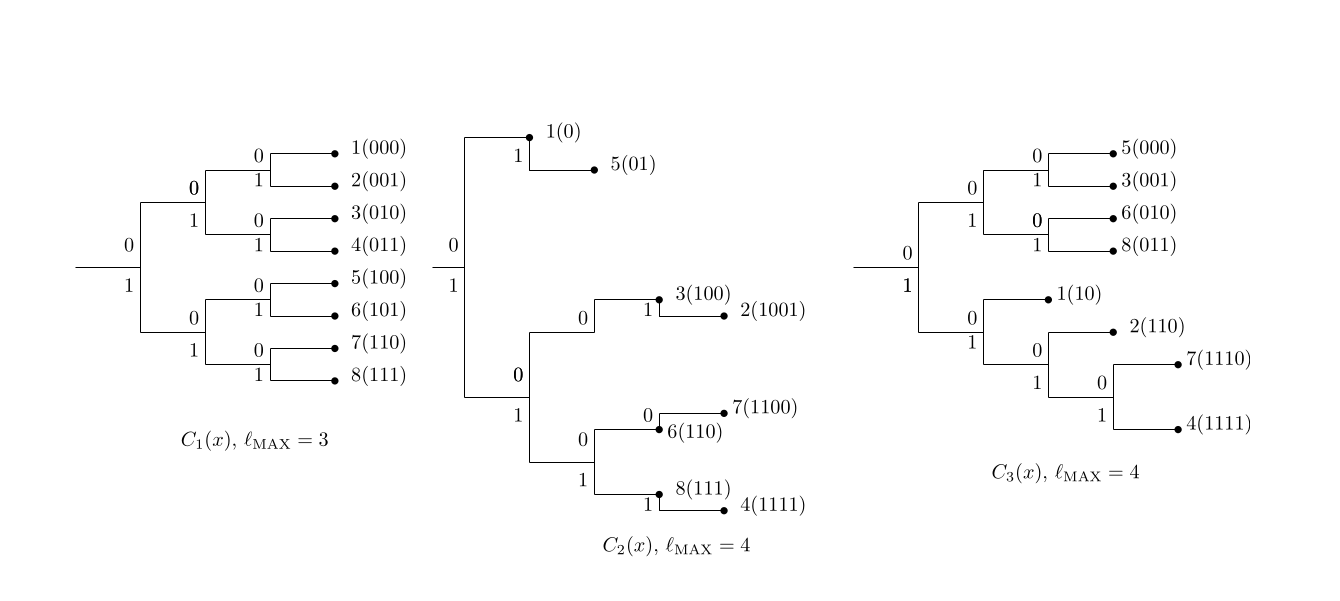
\includegraphics[width=0.9\textwidth]{chapters/06_teoria_informazione/images/c1c2c3tree.png}
    \caption{Rappresentazione ad albero dei codici a prefisso e non a prefisso.}
    \label{fig:alberi_codici}
\end{figure}

Osservando i grafici emerge la regola aurea: \textbf{in un codice a prefisso, le parole di codice possono trovarsi ESCLUSIVAMENTE sui nodi terminali (le foglie) dell'albero.} 
Nell'albero $C_2$, il simbolo 1 (posto sul nodo \texttt{0}) e il simbolo 6 (posto sul nodo \texttt{110}) hanno dei rami figli che proseguono. Questo viola geometricamente la regola del prefisso. Nell'albero $C_3$, tutti i pallini neri sono foglie terminali (nessun ramo prosegue oltre di essi).

\subsubsection{La Disuguaglianza di Kraft}

Questa rappresentazione geometrica ci permette di definire il limite teorico di "abitabilità" dell'albero. 
Un albero binario completo di profondità $\ell_{MAX}$ possiede esattamente $2^{\ell_{MAX}}$ nodi terminali.

Se decidiamo di assegnare una parola di codice a un nodo che si trova a profondità $\ell(x)$, per rispettare la regola del prefisso \textit{dobbiamo tagliare (potare) tutti i rami che partono da quel nodo in giù}. Facendo questo, eliminiamo dall'albero un numero di potenziali foglie pari a $2^{\ell_{MAX} - \ell(x)}$.

Poiché non possiamo tagliare più foglie di quante ne esistano originariamente nell'albero completo, la somma delle foglie eliminate da ogni parola di codice non può superare il totale delle foglie disponibili:
\begin{equation}
\sum_{x \in \mathcal{X}} 2^{\ell_{MAX} - \ell(x)} \le 2^{\ell_{MAX}}
\end{equation}

Dividendo entrambi i membri per $2^{\ell_{MAX}}$, otteniamo la celebre \textbf{Disuguaglianza di Kraft}:
\begin{equation}
\boxed{ \sum_{x \in \mathcal{X}} 2^{-\ell(x)} \le 1 }
\end{equation}

Questo potente teorema fornisce una condizione necessaria e sufficiente. Ci dice matematicamente se un certo insieme di lunghezze di bit $\ell_1, \ell_2, \dots, \ell_M$ è compatibile o meno con la costruzione di un codice istantaneo, ancora prima di provare a disegnare l'albero.

\section{Il Codice di Shannon e il Limite della Compressione}

La Disuguaglianza di Kraft ci fornisce un test matematico per sapere \textit{se} un set di lunghezze può generare un codice istantaneo, ma non ci dice \textit{quali} lunghezze scegliere per ottenere la migliore compressione possibile.

Per risolvere questo problema costruttivo, assumiamo di avere la nostra sorgente con alfabeto $\mathcal{X} = \{x_1, \dots, x_M\}$ e di conoscere perfettamente la legge di probabilità con cui le lettere vengono emesse: $p_X(x_i) = \text{Pr}\{X = x_i\}$.

L'intuizione alla base della Teoria dell'Informazione è che ai simboli meno probabili (che portano molta informazione) debbano corrispondere stringhe binarie più lunghe, e ai simboli molto frequenti stringhe cortissime. Idealmente, vorremmo che la lunghezza $\ell(x_i)$ fosse esattamente pari alla quantità di informazione del simbolo: $\ell_{ideale} = \log_2 \frac{1}{p_X(x_i)}$. 

Tuttavia, nella realtà, non possiamo avere stringhe composte da "1.58 bit". Il numero di bit deve essere necessariamente un intero. Shannon risolve il problema utilizzando la \textbf{funzione tetto} (ceiling), ovvero approssimando la quantità di informazione all'intero superiore.

Si definisce \textbf{Codice di Shannon} un codice in cui la lunghezza della stringa binaria associata al simbolo $x_i$ è:
\begin{equation}
\label{eq:shannon_length}
\ell(x_i) = \left\lceil \log_2 \frac{1}{p_X(x_i)} \right\rceil
\end{equation}

\subsection{Esistenza del Codice di Shannon}

Per definizione matematica, la funzione tetto $\lceil y \rceil$ restituisce un numero intero che è maggiore o uguale a $y$, ma strettamente minore di $y+1$. Traducendo questa regola in algebra per la nostra equazione \ref{eq:shannon_length}, otteniamo la seguente disuguaglianza fondamentale:
\begin{equation} \label{eq:bounds_shannon}
\log_2 \frac{1}{p_X(x_i)} \le \ell(x_i) < \log_2 \frac{1}{p_X(x_i)} + 1
\end{equation}

Ci chiediamo ora: \textit{un codice con queste specifiche lunghezze intere è univocamente decifrabile? Può essere costruito come codice a prefisso?}
Per rispondere, inseriamo le lunghezze $\ell(x_i)$ nella Disuguaglianza di Kraft e verifichiamo se la somma è $\le 1$.

Dalla disuguaglianza \ref{eq:bounds_shannon} sappiamo che $\ell(x_i) \ge \log_2 \frac{1}{p_X(x_i)}$. 
Cambiando il segno, il verso della disuguaglianza si inverte: 
$-\ell(x_i) \le -\log_2 \frac{1}{p_X(x_i)} = \log_2 p_X(x_i)$.

Sostituendo questo esponente nel test di Kraft abbiamo:
\begin{equation}
\sum_{i=1}^{M} 2^{-\ell(x_i)} \le \sum_{i=1}^{M} 2^{\log_2 p_X(x_i)}
\end{equation}
Sappiamo dall'algebra che l'esponenziale in base 2 e il logaritmo in base 2 sono funzioni inverse e si elidono a vicenda ($2^{\log_2(y)} = y$). Pertanto, il termine all'interno della sommatoria diventa semplicemente la probabilità $p_X(x_i)$:
\begin{equation}
\sum_{i=1}^{M} 2^{-\ell(x_i)} \le \sum_{i=1}^{M} p_X(x_i) = 1
\end{equation}

Avendo dimostrato che $\sum 2^{-\ell(x_i)} \le 1$, la disuguaglianza di Kraft è ampiamente soddisfatta. \textbf{Pertanto, esiste sempre matematicamente almeno un codice a prefisso (istantaneo) che adotta le lunghezze del Codice di Shannon.}

\subsection{Entropia e Comprimibilità: Il Primo Teorema di Shannon}

Adesso che sappiamo che il codice esiste ed è decifrabile, calcoliamo le sue prestazioni globali. Vogliamo trovare la lunghezza media del file compresso, ovvero il Valore Atteso delle lunghezze: $L = \mathbb{E}[\ell(X)]$.

Riprendiamo la disuguaglianza fondamentale (Eq. \ref{eq:bounds_shannon}):
\begin{equation*}
\log_2 \frac{1}{p_X(x_i)} \le \ell(x_i) < \log_2 \frac{1}{p_X(x_i)} + 1
\end{equation*}

Per trasformare questa espressione nel calcolo di una media statistica globale, moltiplichiamo tutti i termini per la probabilità $p_X(x_i)$ e sommiamo su tutti i simboli $M$ dell'alfabeto:
\begin{equation}
\sum_{i=1}^{M} p_X(x_i) \log_2 \frac{1}{p_X(x_i)} \le \sum_{i=1}^{M} p_X(x_i) \ell(x_i) < \sum_{i=1}^{M} p_X(x_i) \left( \log_2 \frac{1}{p_X(x_i)} + 1 \right)
\end{equation}

Analizziamo i tre blocchi di questa disequazione espandendo il termine a destra:
\begin{equation}
\underbrace{\sum_{i=1}^{M} p_X(x_i) \log_2 \frac{1}{p_X(x_i)}}_{H(X)} \le \underbrace{\sum_{i=1}^{M} p_X(x_i) \ell(x_i)}_{L} < \underbrace{\sum_{i=1}^{M} p_X(x_i) \log_2 \frac{1}{p_X(x_i)}}_{H(X)} + \underbrace{\sum_{i=1}^{M} p_X(x_i)}_{1}
\end{equation}

Riconosciamo immediatamente le definizioni a noi note (dove la somma di tutte le probabilità fa ovviamente 1). Arriviamo così al risultato fondamentale della codifica di sorgente:
\begin{equation}
\boxed{ H(X) \le L < H(X) + 1 }
\end{equation}

\subsubsection{Interpretazione del Teorema}
Questa relazione, apparentemente semplice, racchiude due verità ingegneristiche assolute:
\begin{enumerate}
    \item \textbf{Il limite invalicabile della compressione ($L \ge H(X)$):} Nessun codice decifrabile al mondo potrà mai avere una lunghezza media per simbolo inferiore all'Entropia della sorgente. L'Entropia rappresenta l'essenza pura dell'informazione, il suo "peso atomico". Se si cerca di comprimere un file a un livello inferiore alla sua entropia, si perderanno inesorabilmente dei dati e il file originale non sarà più ricostruibile.
    \item \textbf{L'efficienza del Codice di Shannon ($L < H(X) + 1$):} Utilizzando la semplicissima tecnica dell'arrotondamento all'intero superiore ideata da Shannon, abbiamo la garanzia assoluta di ottenere un codice le cui prestazioni distano \textit{al massimo meno di 1 bit per simbolo} dall'efficienza perfetta ideale.
\end{enumerate}

\section{Codici a Prefisso Ottimi: L'Algoritmo di Huffman}

Abbiamo visto che il Codice di Shannon garantisce una lunghezza media che dista al massimo 1 bit dall'entropia. Tuttavia, in ingegneria vogliamo trovare la soluzione \textit{migliore in assoluto}. Vogliamo costruire un codice a prefisso la cui lunghezza media $L$ sia il minimo matematicamente possibile per una data sorgente. 
Questo risultato si ottiene tramite l'**Algoritmo di Huffman**.

L'algoritmo costruisce l'albero di codifica "dal basso verso l'alto" (dalle foglie verso la radice) seguendo questi semplici passi iterativi:
\begin{enumerate}
    \item Si dispongono verticalmente i simboli dell'alfabeto in ordine di probabilità decrescente.
    \item Si raggruppano i due simboli \textit{meno probabili} in un nuovo "macrosimbolo" (un nodo genitore). A questo nuovo nodo si assegna una probabilità pari alla somma delle probabilità dei due nodi figli. Questo passaggio riduce di fatto la cardinalità dell'alfabeto di un'unità.
    \item Si riordina il nuovo alfabeto e si ripete il passo precedente, unendo sempre i due elementi con probabilità minore, fino a quando non si arriva alla radice dell'albero, che avrà necessariamente probabilità $1$.
    \item Infine, partendo dalla radice e scendendo verso le foglie, si assegna convenzionalmente il bit `0` a un ramo e il bit `1` all'altro. La parola di codice per ogni simbolo si ottiene leggendo la sequenza di bit dalla radice fino al nodo terminale corrispondente.
\end{enumerate}

\subsection{Esempio Pratico e Inserimento Alberi}

Consideriamo un alfabeto di 8 simboli $\mathcal{X} = \{1,2,3,4,5,6,7,8\}$ e analizziamo il comportamento di Huffman su due diverse distribuzioni di probabilità, $p_1(x)$ e $p_2(x)$:
\begin{equation*}
    p_1(x) = \left\{ \frac{1}{4}, \frac{1}{4}, \frac{1}{8}, \frac{1}{8}, \frac{1}{16}, \frac{1}{16}, \frac{1}{16}, \frac{1}{16} \right\}, \quad 
    p_2(x) = \left\{ \frac{1}{3}, \frac{1}{9}, \frac{1}{9}, \frac{1}{9}, \frac{1}{27}, \frac{2}{27}, \frac{1}{6}, \frac{1}{18} \right\}
\end{equation*}

\begin{figure}[htbp]
    \centering
    % Sostituisci "huffman_p1.png" con il nome reale del tuo file per il primo albero
    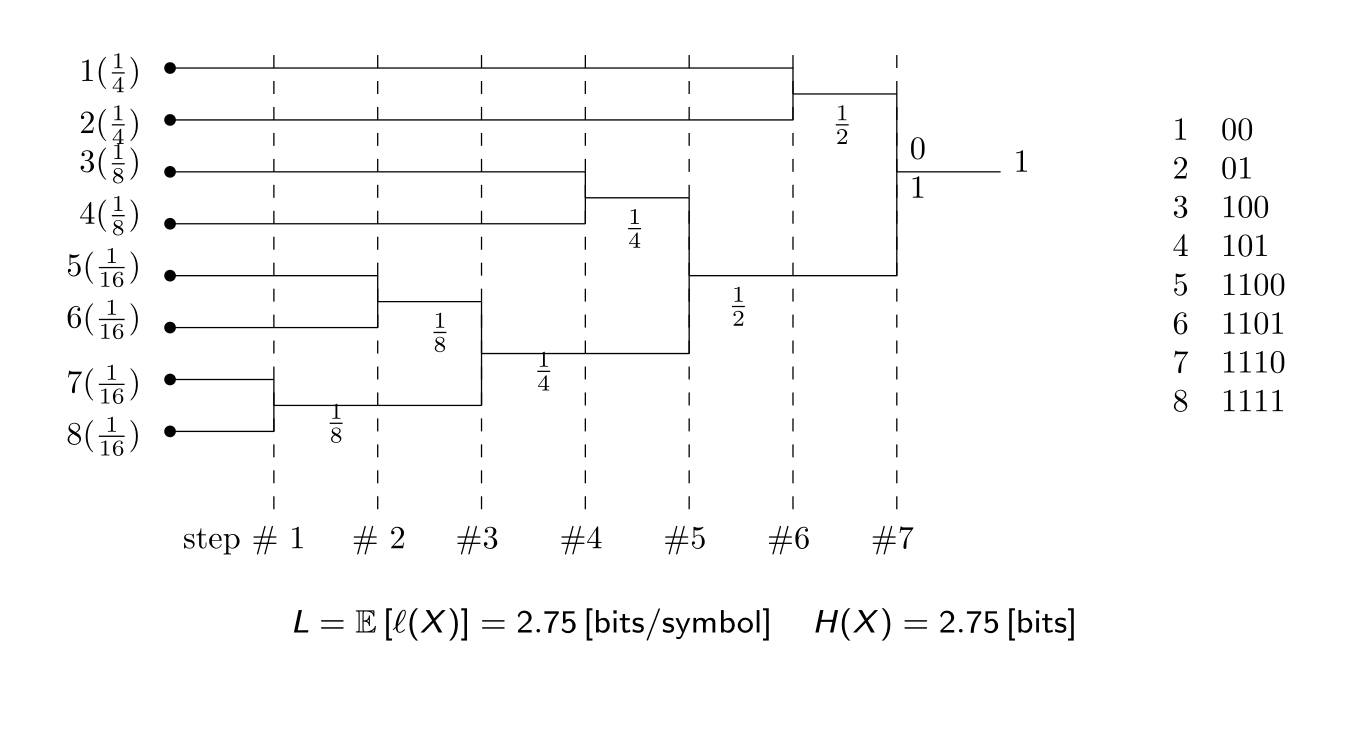
\includegraphics[width=0.85\textwidth]{chapters/06_teoria_informazione/images/huffman1.png}
    \caption{Albero di Huffman generato per la distribuzione $p_1(x)$.}
    \label{fig:huffman1}
\end{figure}

\begin{figure}[htbp]
    \centering
    % Sostituisci "huffman_p2.png" con il nome reale del tuo file per il secondo albero
    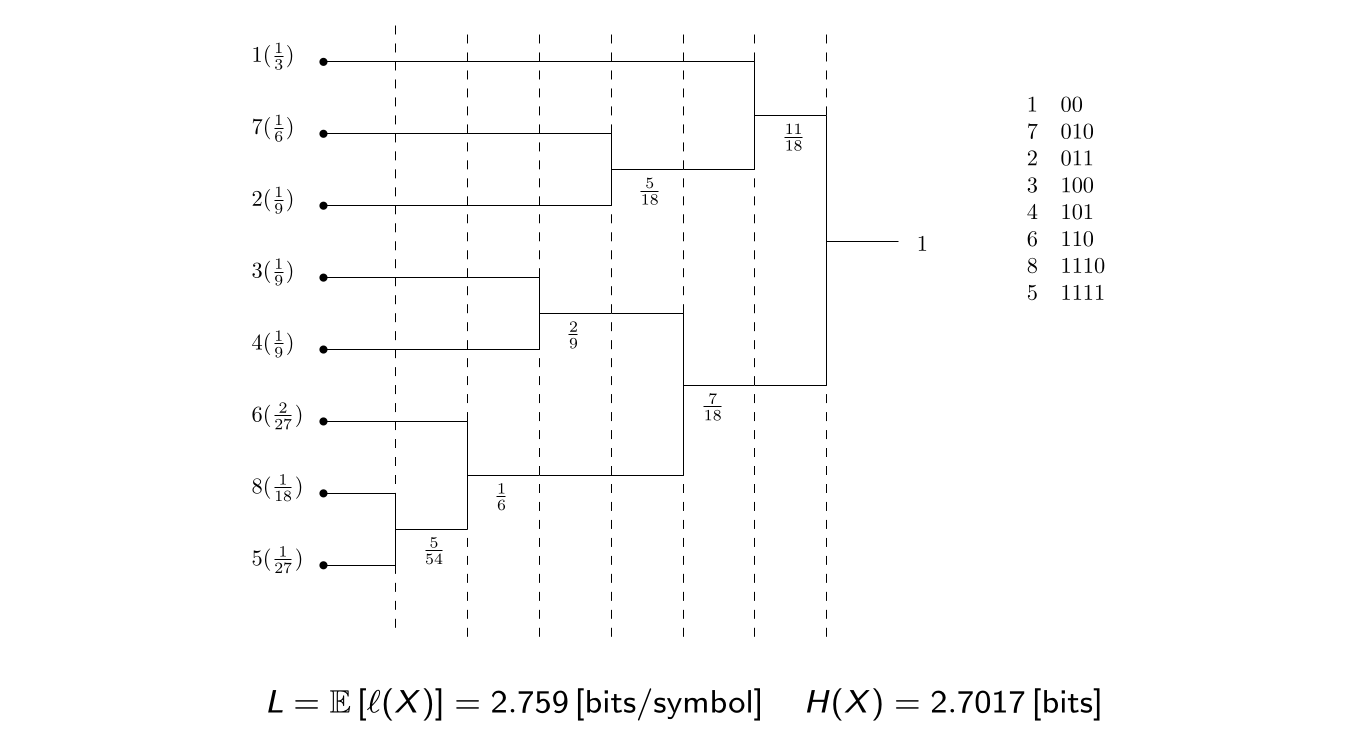
\includegraphics[width=0.85\textwidth]{chapters/06_teoria_informazione/images/huffman2.png}
    \caption{Albero di Huffman generato per la distribuzione $p_2(x)$.}
    \label{fig:huffman2}
\end{figure}

\subsection{Analisi dell'Ottimalità e Limite Entropico}

Osservando i risultati della codifica di Huffman, possiamo trarre delle considerazioni:
\begin{itemize}
    \item \textbf{Non unicità:} L'albero di Huffman non è unico. A parità di probabilità, potremmo scambiare l'assegnazione di `0` e `1` sui rami, o l'ordine con cui uniamo simboli che hanno la stessa identica probabilità. Tuttavia, la lunghezza media $L$ risultante sarà sempre la stessa e sempre la minima possibile.
    \item \textbf{Compressione Perfetta (Caso $p_1$):} Nel primo caso, calcolando l'entropia della sorgente otteniamo $H(X) = 2.75$ bit. La lunghezza media del codice di Huffman risulta esattamente $L = 2.75$ bit/simbolo. Il codice ha raggiunto il limite teorico invalicabile ($L = H(X)$).
    \item \textbf{Compressione Imperfetta (Caso $p_2$):} Nel secondo caso, l'entropia è $H(X) \approx 2.7017$, ma Huffman si ferma a $L \approx 2.759$. Questo ci dimostra che l'uguaglianza $L = H(X)$ non è sempre raggiungibile.
\end{itemize}

Ci chiediamo: qual è la condizione matematica rigorosa affinché Huffman raggiunga esattamente l'entropia? 
La dimostrazione richiede che le probabilità di emissione siano esattamente delle potenze negative di 2 (ovvero distribuzioni diidiche). Esplicitiamo matematicamente questa condizione:
Assumiamo che la probabilità sia della forma $p_X(x) = 2^{-\ell(x)}$.
Se calcoliamo il logaritmo in base 2 dell'inverso della probabilità otteniamo:
\begin{equation}
\log_2 \frac{1}{p_X(x)} = \log_2 \frac{1}{2^{-\ell(x)}} = \log_2 \left( 2^{\ell(x)} \right) = \ell(x)
\end{equation}
Sostituendo questo risultato nella formula del valore atteso della lunghezza, troviamo:
\begin{equation}
L = \mathbb{E}[\ell(X)] = \sum_{x \in \mathcal{X}} p_X(x) \cdot \ell(x) = \sum_{x \in \mathcal{X}} p_X(x) \cdot \log_2 \frac{1}{p_X(x)} \equiv H(X)
\end{equation}
Solo se le probabilità obbediscono a questa rigida legge esponenziale il codice sarà "perfetto" senza sprecare frazioni di bit.

% ==========================================
% NUOVO ARGOMENTO: COPPIE DI VARIABILI
% ==========================================

\section{Estensione a Coppie di Variabili Aleatorie}

Finora abbiamo analizzato sorgenti che emettono un singolo simbolo alla volta. Nella realtà, i sistemi elaborano spesso flussi di dati correlati (es. pixel adiacenti in un'immagine, o canali stereo audio).
Siano $X$ e $Y$ due variabili aleatorie discrete associate agli alfabeti $\mathcal{X}$ e $\mathcal{Y}$. Definiamo la loro interazione tramite la \textbf{Probability Mass Function (PMF) Congiunta}: $p_{X,Y}(x,y) = \text{Pr}\{X=x \text{ e } Y=y\}$.

Vogliamo misurare l'incertezza media globale quando osserviamo simultaneamente \textit{entrambe} le variabili.

\subsection{Entropia Congiunta}
Generalizzando il concetto di entropia a due dimensioni, definiamo l'\textbf{Entropia Congiunta} $H(X,Y)$ estendendo la doppia sommatoria su tutti i possibili incroci degli eventi:
\begin{equation}
\label{eq:joint_entropy}
H(X, Y) = \mathbb{E}_{X,Y} \left[ \log \frac{1}{p_{X,Y}(X,Y)} \right] = \sum_{x \in \mathcal{X}} \sum_{y \in \mathcal{Y}} p_{X,Y}(x,y) \log \frac{1}{p_{X,Y}(x,y)}
\end{equation}

\subsubsection{Il caso di Indipendenza Statistica}
Cosa succede all'entropia se le due variabili non hanno assolutamente nulla a che fare l'una con l'altra (es. estrarre un dado e lanciare una moneta)? 
Dalla teoria della probabilità, sappiamo che due eventi sono \textbf{indipendenti} se e solo se la loro probabilità congiunta è il prodotto delle probabilità marginali: $p_{X,Y}(x,y) = p_X(x) \cdot p_Y(y)$.

Sostituiamo questa definizione all'interno dell'argomento del logaritmo nella \ref{eq:joint_entropy} ed esplodiamo i calcoli sfruttando le proprietà dei logaritmi ($\log(a \cdot b) = \log a + \log b$):
\begin{align}
H(X, Y) &= \mathbb{E} \left[ \log \frac{1}{p_X(X) \cdot p_Y(Y)} \right] \nonumber \\
        &= \mathbb{E} \left[ \log \left( \frac{1}{p_X(X)} \right) + \log \left( \frac{1}{p_Y(Y)} \right) \right]
\end{align}
Essendo l'operatore di Valore Atteso ($\mathbb{E}$) un operatore lineare, il valore atteso di una somma è la somma dei valori attesi:
\begin{align}
H(X,Y)  &= \mathbb{E} \left[ \log \frac{1}{p_X(X)} \right] + \mathbb{E} \left[ \log \frac{1}{p_Y(Y)} \right] \nonumber \\
        &= H(X) + H(Y)
\end{align}
Abbiamo dimostrato che, in caso di totale indipendenza, l'incertezza globale del sistema è semplicemente la somma delle incertezze dei singoli componenti.

\subsection{Entropia Condizionale e Regola della Catena}

Se invece le variabili \textit{sono} dipendenti (es. il cielo è nuvoloso $\implies$ probabilità che piova), conoscere il valore di una variabile riduce l'incertezza sull'altra.
Ricorriamo alla \textbf{legge della probabilità composta} (o Teorema di Bayes ristretto):
\begin{equation}
p_{X,Y}(x,y) = p_{Y|X}(y|x) \cdot p_X(x) = p_{X|Y}(x|y) \cdot p_Y(y)
\end{equation}

Sostituiamo la scomposizione $p_{Y|X}(y|x) p_X(x)$ nella definizione di Entropia Congiunta per derivare la \textbf{Regola della Catena}. Di nuovo, espandiamo passo dopo passo i logaritmi e l'aspettazione:
\begin{align}
H(X, Y) &= \mathbb{E} \left[ \log \frac{1}{p_X(X) \cdot p_{Y|X}(Y|X)} \right] \nonumber \\
        &= \mathbb{E} \left[ \log \frac{1}{p_X(X)} + \log \frac{1}{p_{Y|X}(Y|X)} \right] \nonumber \\
        &= \mathbb{E} \left[ \log \frac{1}{p_X(X)} \right] + \mathbb{E} \left[ \log \frac{1}{p_{Y|X}(Y|X)} \right]
\end{align}

Il primo termine è palesemente l'entropia marginale $H(X)$. 
Il secondo termine definisce una nuova grandezza, l'\textbf{Entropia Condizionale} $H(Y|X)$, ovvero l'incertezza residua su $Y$ sapendo di aver già osservato $X$. 
Scritta in forma estesa (esplicitando il Valore Atteso), la formula appare così:
\begin{equation}
\label{eq:cond_entropy}
H(Y|X) = \sum_{x \in \mathcal{X}} \sum_{y \in \mathcal{Y}} p_{X,Y}(x,y) \log \frac{1}{p_{Y|X}(y|x)}
\end{equation}

\subsubsection*{Approfondimento: Perché usiamo la probabilità congiunta come "peso"?}

A questo punto, osservando l'equazione \ref{eq:cond_entropy}, sorge spontaneo uno dei dubbi più comuni e legittimi nello studio dell'entropia: \textit{perché come peso della doppia sommatoria utilizziamo la probabilità congiunta $p_{X,Y}$ e non la probabilità condizionata $p_{Y|X}$?}

La risposta breve è che l'entropia condizionale $H(Y|X)$ \textbf{non} misura l'incertezza di $Y$ dato un \textit{singolo e specifico} valore di $X$, ma rappresenta l'incertezza \textit{media} di $Y$ calcolata su \textit{tutti i possibili} valori che $X$ può assumere.

Per capire esattamente da dove spunta la probabilità congiunta, dobbiamo scomporre il calcolo logico in due passaggi.

\paragraph{1. L'entropia dato un evento specifico $X=x$}
Se noi sapessimo con assoluta certezza che la variabile $X$ ha appena assunto un valore specifico (chiamiamolo $x$), calcoleremmo l'entropia di $Y$ usando giustamente la probabilità condizionata come peso. Questa quantità puntuale si indica con $H(Y|X=x)$:
\begin{equation}
H(Y|X=x) = \sum_{y \in \mathcal{Y}} p_{Y|X}(y|x) \log \frac{1}{p_{Y|X}(y|x)}
\end{equation}

\paragraph{2. La media globale su tutti i possibili valori di $X$}
Il problema è che·noi non sappiamo quale valore assumerà $X$. Quindi, per definire l'entropia condizionale globale $H(Y|X)$, dobbiamo effettuare una media pesata di tutte le possibili entropie $H(Y|X=x)$, usando come peso la probabilità che si verifichi quel determinato contesto $x$ (ovvero la probabilità marginale $p_X(x)$):
\begin{equation}
H(Y|X) = \sum_{x \in \mathcal{X}} p_X(x) H(Y|X=x)
\end{equation}

\paragraph{3. La sostituzione finale}
Ora sostituiamo la prima formula all'interno della seconda:
\begin{equation}
H(Y|X) = \sum_{x \in \mathcal{X}} p_X(x) \left[ \sum_{y \in \mathcal{Y}} p_{Y|X}(y|x) \log \frac{1}{p_{Y|X}(y|x)} \right]
\end{equation}
Poiché il termine $p_X(x)$ non dipende dall'indice della sommatoria interna $y$, possiamo portarlo dentro le parentesi quadre:
\begin{equation}
H(Y|X) = \sum_{x \in \mathcal{X}} \sum_{y \in \mathcal{Y}} \left[ p_X(x) \cdot p_{Y|X}(y|x) \right] \log \frac{1}{p_{Y|X}(y|x)}
\end{equation}
Per la legge della probabilità composta, il termine tra parentesi quadre $p_X(x) \cdot p_{Y|X}(y|x)$ è l'esatta definizione della probabilità congiunta $p_{X,Y}(x,y)$.

\begin{quote}
\textbf{In sintesi:} Si usa la probabilità congiunta $p_{X,Y}(x,y)$ perché essa racchiude elegantemente in un unico termine due concetti: quanto è probabile l'evento condizionante $X=x$, moltiplicato per quanto è probabile l'evento $Y=y$ dato quel preciso contesto.
\end{quote}

In conclusione, la Regola della Catena stabilisce che l'incertezza totale di una coppia di variabili si può sempre scomporre nell'incertezza della prima, più l'incertezza residua della seconda sapendo la prima:
\begin{equation}
\boxed{ H(X,Y) = H(X) + H(Y|X) = H(Y) + H(X|Y) }
\end{equation}

\section{Mutua Informazione tra Variabili Aleatorie}

Riprendiamo la Regola della Catena appena dimostrata per l'entropia congiunta di due variabili aleatorie $(X, Y) \sim p_{X,Y}(x,y)$:
\begin{equation*}
    H(X, Y) = H(X) + H(Y|X) = H(Y) + H(X|Y)
\end{equation*}

Prendendo le ultime due parti di questa uguaglianza e riordinando i termini (portando le entropie marginali da una parte e quelle condizionate dall'altra), otteniamo una simmetria molto interessante:
\begin{equation}
    H(X) - H(X|Y) = H(Y) - H(Y|X)
\end{equation}

Questa quantità prende il nome di \textbf{Mutua Informazione} tra $X$ e $Y$ e si indica con $I(X;Y)$:
\begin{equation}
\label{eq:mutual_info_def}
    I(X;Y) = H(X) - H(X|Y)
\end{equation}

\subsubsection*{Significato Intuitivo}
Cosa rappresenta la formula $H(X) - H(X|Y)$? 
$H(X)$ è la mia incertezza iniziale su $X$ prima di fare qualsiasi esperimento. $H(X|Y)$ è l'incertezza che mi "rimane" su $X$ dopo aver osservato il valore di $Y$. 
La loro differenza rappresenta quindi \textbf{l'incertezza che è stata rimossa} (o l'informazione che è stata acquisita) su $X$ grazie al fatto di aver osservato $Y$. In altre parole, $I(X;Y)$ misura il grado di dipendenza statistica (e quindi di predicibilità reciproca) tra le due variabili.

\subsection{Espansione Matematica: Il legame con la KL Divergence}

Vogliamo ora manipolare l'equazione \ref{eq:mutual_info_def} per esprimerla in termini di probabilità congiunta e marginale. 

Scriviamo l'espressione in forma di Valore Atteso. Per poter sommare i due valori attesi, dobbiamo calcolarli entrambi sullo stesso dominio congiunto $(X,Y)$. Ricordiamo che la media marginale $\mathbb{E}_X[\cdot]$ equivale a calcolare la media congiunta $\mathbb{E}_{X,Y}[\cdot]$ poiché la somma su $Y$ restituisce 1.
\begin{equation}
    I(X;Y) = \mathbb{E}_{X,Y} \left[ \log \frac{1}{p_X(X)} \right] - \mathbb{E}_{X,Y} \left[ \log \frac{1}{p_{X|Y}(X|Y)} \right]
\end{equation}

Sfruttiamo la linearità del valore atteso per raggruppare i due termini sotto un unico operatore $\mathbb{E}$:
\begin{equation}
    I(X;Y) = \mathbb{E}_{X,Y} \left[ \log \frac{1}{p_X(X)} - \log \frac{1}{p_{X|Y}(X|Y)} \right]
\end{equation}

Applichiamo la proprietà dei logaritmi ($\log A - \log B = \log \frac{A}{B}$):
\begin{equation}
    I(X;Y) = \mathbb{E}_{X,Y} \left[ \log \left( \frac{\frac{1}{p_X(X)}}{\frac{1}{p_{X|Y}(X|Y)}} \right) \right] = \mathbb{E}_{X,Y} \left[ \log \frac{p_{X|Y}(X|Y)}{p_X(X)} \right]
\end{equation}

A questo punto usiamo il Teorema di Bayes (definizione di probabilità condizionata), secondo cui $p_{X|Y}(x|y) = \frac{p_{X,Y}(x,y)}{p_Y(y)}$. Sostituiamo il numeratore:
\begin{equation}
    I(X;Y) = \mathbb{E}_{X,Y} \left[ \log \frac{\frac{p_{X,Y}(X,Y)}{p_Y(Y)}}{p_X(X)} \right] = \mathbb{E}_{X,Y} \left[ \log \frac{p_{X,Y}(X,Y)}{p_X(X)p_Y(Y)} \right]
\end{equation}

\textbf{Osservazione fondamentale:} Se guardiamo attentamente la formula appena ottenuta e la confrontiamo con la definizione di Entropia Relativa (Divergenza di Kullback-Leibler) studiata in precedenza, notiamo che sono \textit{identiche}. 
La Mutua Informazione non è altro che la Distanza di Kullback-Leibler tra la vera probabilità congiunta $p_{X,Y}(x,y)$ e la probabilità fittizia $p_X(x)p_Y(y)$ che avremmo se le due variabili fossero completamente indipendenti:
\begin{equation}
    \boxed{ I(X;Y) = D( p_{X,Y}(x,y) \parallel p_X(x)p_Y(y) ) }
\end{equation}

\subsection{Conseguenze e Teoremi (Il Condizionamento non aumenta l'Entropia)}

Aver dimostrato che la Mutua Informazione è di fatto una Divergenza KL ci permette di ereditare istantaneamente tutti i potenti teoremi associati alla divergenza $D(p \parallel q)$:

\begin{enumerate}
    \item \textbf{Non negatività:} Sappiamo che $D(p \parallel q) \ge 0$ in ogni caso. Di conseguenza:
    \begin{equation}
        I(X;Y) \ge 0
    \end{equation}
    
    \item \textbf{Il Condizionamento non aumenta l'Entropia:} Sostituendo la disuguaglianza appena trovata nella definizione originale ($I(X;Y) = H(X) - H(X|Y) \ge 0$), otteniamo un risultato filosoficamente e matematicamente imponente:
    \begin{equation}
        H(X) \ge H(X|Y) \quad \text{e per simmetria} \quad H(Y) \ge H(Y|X)
    \end{equation}
    \textit{Significato pratico:} Aggiungere informazione (condizionare rispetto a una nuova variabile $Y$) può solo ridurre, o al limite lasciare inalterata, l'incertezza che abbiamo sul sistema. \textbf{L'informazione non può mai fare danni} aumentando la nostra incertezza.
    
    \item \textbf{Condizione per l'Indipendenza:} Sappiamo che la Divergenza KL è zero se e solo se le due distribuzioni sono identiche ($D(p \parallel q)=0 \iff p=q$). Pertanto:
    \begin{equation}
        I(X;Y) = 0 \iff p_{X,Y}(x,y) = p_X(x)p_Y(y)
    \end{equation}
    Questo significa che la mutua informazione tra due variabili è nulla \textbf{se e solo se} esse sono statisticamente indipendenti.
    Se due variabili sono indipendenti, sapere $Y$ non mi dice assolutamente nulla di nuovo su $X$. Matematicamente, l'entropia condizionale collassa nell'entropia marginale:
    \begin{equation}
        H(X|Y) = H(X) \quad \text{e} \quad H(Y|X) = H(Y)
    \end{equation}
\end{enumerate}
% ==========================================
% NUOVO ARGOMENTO: SORGENTI E PROCESSI
% ==========================================

\section{Modellizzazione delle Sorgenti di Informazione}

Fino a questo momento abbiamo calcolato l'entropia di singole variabili o di coppie isolate. Tuttavia, in uno scenario di telecomunicazioni reale, un trasmettitore non emette un solo simbolo per poi spegnersi, ma genera un flusso continuo di dati nel tempo. 

Una generica sorgente di informazione è modellabile matematicamente come un generatore che produce una sequenza temporale di variabili aleatorie $\{X_i\}_{i \in \mathbb{Z}}$. Questa sequenza prende il nome di \textbf{processo aleatorio tempo-discreto}.

\begin{center}
\vspace{0.3cm}
\begin{tikzpicture}[>=stealth]
    % Blocco Sorgente
    \node[draw, fill=blue, text=white, minimum width=3.5cm, minimum height=2cm, font=\large\bfseries] (source) {Sorgente};
    % Freccia in uscita
    \draw[->, blue, very thick] (source.east) -- +(3,0) node[right, text=black, font=\normalsize] {$\dots, X_{-1}, X_0, X_1, \dots, X_n, \dots$};
\end{tikzpicture}
\vspace{0.3cm}
\end{center}

\subsection{Ipotesi Semplificative del Modello}

Assumeremo che il processo generato dalla sorgente rispetti tre ipotesi fondamentali:
\begin{enumerate}
    \item \textbf{Ampiezza discreta:} L'alfabeto $\mathcal{X}$ da cui vengono estratti i simboli ha cardinalità finita (es. codice binario, alfabeto testuale).
    \item \textbf{Stazionarietà in senso stretto (di ordine qualsiasi):} Le leggi statistiche che governano la sorgente non cambiano col passare del tempo. La probabilità di osservare una certa sequenza oggi è identica alla probabilità di osservarla domani.
    \item \textbf{Caratterizzazione completa:} Si assume che tutte le PMF (Probability Mass Function) congiunte di qualsiasi ordine siano note a priori all'analista.
\end{enumerate}

\subsection{Sorgenti Senza Memoria (DMS)}

All'interno della famiglia dei processi stazionari, esiste una sottoclasse di fondamentale importanza teorica. 
Una sorgente si dice \textbf{senza memoria} se i simboli emessi sono tra loro \textit{statisticamente indipendenti}. In altre parole, il simbolo $X_k$ che la sorgente sta per emettere non è in alcun modo influenzato dalla conoscenza dei simboli $X_{k-1}, X_{k-2}$ emessi in precedenza. 

L'acronimo \textbf{DMS} (\textit{Discrete Memoryless Source}).

\subsection{Contenuto Informativo di una DMS (Entropia di Blocco)}

Vogliamo ora calcolare quanta informazione è contenuta in un intero blocco di simboli consecutivi emessi da una DMS. 
Consideriamo un blocco di lunghezza $n$, che possiamo indicare come un vettore aleatorio: $\mathbf{X}^n = (X_1, X_2, \dots, X_n) \in \mathcal{X}^n$.

Applicando per generalizzazione la definizione di entropia congiunta vista nel capitolo precedente, l'entropia del blocco è il valore atteso del logaritmo dell'inverso della PMF congiunta di ordine $n$:
\begin{equation}
    H(\mathbf{X}^n) = H(X_1, X_2, \dots, X_n) = \sum_{\mathbf{x}^n \in \mathcal{X}^n} p_{\mathbf{X}^n}(\mathbf{x}^n) \log \left[ \frac{1}{p_{\mathbf{X}^n}(\mathbf{x}^n)} \right]
\end{equation}

Sviluppiamo matematicamente questa espressione sfruttando la definizione di DMS. Poiché la sorgente è \textit{senza memoria}, le variabili sono indipendenti. Di conseguenza, la probabilità congiunta di osservare l'intero blocco è semplicemente il prodotto delle probabilità marginali dei singoli simboli:
\begin{equation}
    p_{\mathbf{X}^n}(\mathbf{x}^n) = \prod_{i=1}^{n} p_{X_i}(x_i)
\end{equation}

Sostituendo questo prodotto all'interno del calcolo del valore atteso (Entropia) e sfruttando le proprietà dei logaritmi, i passaggi si svolgono come segue:
\begin{align}
    H(\mathbf{X}^n) &= \mathbb{E} \left[ \log \frac{1}{\prod_{i=1}^{n} p_{X_i}(X_i)} \right] \nonumber \\
                    &= \mathbb{E} \left[ \sum_{i=1}^{n} \log \frac{1}{p_{X_i}(X_i)} \right] \nonumber \\
                    &= \sum_{i=1}^{n} \mathbb{E} \left[ \log \frac{1}{p_{X_i}(X_i)} \right] \nonumber \\
                    &= \sum_{i=1}^{n} H(X_i)
\end{align}

Infine, ricordiamo che la sorgente è \textit{stazionaria}, il che significa che l'entropia marginale di ogni singolo istante di tempo è costante e identica a quella del primo simbolo ($H(X_i) = H(X_1)$ per ogni $i$). La somma di $n$ termini identici ci porta al risultato finale:
\begin{equation}
    \boxed{ H(\mathbf{X}^n) = n \cdot H(X_1) }
\end{equation}
L'entropia di un blocco di $n$ simboli generati da una sorgente senza memoria è esattamente $n$ volte l'entropia di un singolo simbolo.

\subsection{Il Tasso Entropico (Entropy Rate)}

Per valutare il flusso di informazione di un processo in modo indipendente dalla lunghezza specifica del blocco $n$ che stiamo analizzando, si introduce una metrica asintotica chiamata \textbf{Tasso Entropico} (o \textit{Entropy Rate}). 

Esso è definito come il limite per $n$ che tende all'infinito della quantità media di informazione trasportata da un singolo simbolo all'interno di un blocco infinito:
\begin{equation}
    H_\infty(\mathcal{X}) = \lim_{n \to \infty} \frac{H(\mathbf{X}^n)}{n}
\end{equation}

Sostituendo il risultato ottenuto nel paragrafo precedente per le DMS ($H(\mathbf{X}^n) = n H(X_1)$), il limite diventa banale:
\begin{equation}
    H_\infty(\mathcal{X}) = \lim_{n \to \infty} \frac{n \cdot H(X_1)}{n} = H(X_1)
\end{equation}

\textbf{Conclusione fisica:} Per una sorgente Discreta Senza Memoria, il tasso entropico coincide esattamente con l'entropia della singola emissione marginale. In termini pratici, questo significa che in una DMS non c'è "ridondanza nascosta" tra un simbolo e l'altro; osservare blocchi di dati molto lunghi non ci aiuterà a comprimere i dati meglio di quanto potremmo fare comprimendo simbolo per simbolo, poiché ogni nuova emissione porta con sé una quantità di incertezza "fresca" e totalmente indipendente dal passato.

% ==========================================
% NUOVO ARGOMENTO: SORGENTI CON MEMORIA
% ==========================================

\section{Sorgenti con Memoria}

Rimuoviamo ora l'ipotesi forte di indipendenza tra i simboli (DMS), conservando unicamente l'ipotesi di stazionarietà. In una \textbf{sorgente con memoria}, la probabilità che venga emesso un certo simbolo dipende dai simboli che lo hanno preceduto nel tempo. Esempi classici sono il linguaggio umano (la probabilità che la lettera 'U' segua la lettera 'Q' è altissima) o il meteo.

Per modellare questa situazione, ricordiamo la \textbf{Legge di Bayes} generalizzata a $n$ variabili (nota come regola della catena per le probabilità). La probabilità congiunta di osservare un'intera sequenza $\mathbf{x}^n$ si può fattorizzare condizionando ogni simbolo al suo intero passato:
\begin{equation}
    p_{\mathbf{X}^n}(\mathbf{x}^n) = p_{X_1}(x_1) \cdot p_{X_2|X_1}(x_2|x_1) \cdot p_{X_3|X_2,X_1}(x_3|x_2,x_1) \dots p_{X_n|X_{n-1},\dots,X_1}(x_n|x_{n-1},\dots,x_1)
\end{equation}

Di conseguenza, applicando lo stesso principio logico esplorato con le coppie di variabili aleatorie, l'entropia congiunta dell'intero blocco di dati $\mathbf{X}^n$ si espande in una somma di entropie condizionate:
\begin{equation}
    H(\mathbf{X}^n) = H(X_1) + H(X_2|X_1) + \dots + H(X_n|X_{n-1}, \dots, X_1)
\end{equation}
Che possiamo riscrivere in forma compatta con una sommatoria:
\begin{equation}
    H(\mathbf{X}^n) = \sum_{i=1}^{n} H(X_i | X_{i-1}, \dots, X_1)
\end{equation}

\subsection{Il Concetto di Innovazione}

Soffermiamoci sul generico termine della sommatoria, definendolo esplicitamente tramite il valore atteso:
\begin{equation}
    H(X_i | X_{i-1}, \dots, X_1) = \sum_{\mathbf{x}^i \in \mathcal{X}^i} p_{\mathbf{X}^i}(\mathbf{x}^i) \log \left( \frac{1}{p_{X_i | X_{i-1}, \dots, X_1}(x_i | x_{i-1}, \dots, x_1)} \right)
\end{equation}

Questa quantità ha un significato fisico e informatico profondissimo: rappresenta \textbf{l'incertezza residua sul simbolo $X_i$ una volta che tutti i simboli precedenti sono noti}. 
In altre parole, rappresenta quella parte di informazione trasportata dall'$i$-esimo simbolo che \textit{non era assolutamente predicibile} guardando al passato. Nella teoria dei segnali, questa quantità di informazione "fresca" o "nuova" prende il nome di \textbf{Innovazione}.

\section{Tasso Entropico di Sorgenti con Memoria}

Vogliamo ora calcolare il tasso entropico $H_\infty(\mathcal{X})$ per questa sorgente, ovvero l'incertezza media per simbolo valutata su una sequenza di lunghezza infinita:
\begin{equation}
    H_\infty(\mathcal{X}) = \lim_{n \to \infty} \frac{H(\mathbf{X}^n)}{n} 
\end{equation}

Sostituendo l'entropia di blocco con la sommatoria appena ricavata tramite la regola della catena, otteniamo:
\begin{equation}
\label{eq:rate_sum}
    H_\infty(\mathcal{X}) = \lim_{n \to \infty} \frac{1}{n} \sum_{i=1}^{n} H(X_i | X_{i-1}, \dots, X_1)
\end{equation}

Dal punto di vista analitico, abbiamo il limite di una media aritmetica di termini. Per risolvere questa operazione in modo elegante, ricorriamo a uno strumento dell'analisi matematica: il Teorema della media di Cesàro.

\subsection{Il Teorema di Cesàro}

Il teorema stabilisce che se abbiamo una successione numerica $\{b_n\}$ che converge a un limite ben preciso $b$, allora anche la successione formata dalle sue \textit{medie aritmetiche} convergerà allo stesso identico limite $b$.
\begin{equation*}
    \lim_{n \to \infty} b_n = b \implies \lim_{n \to \infty} \frac{1}{n} \sum_{i=1}^{n} b_i = b
\end{equation*}

\subsubsection{Applicazione al Tasso Entropico}
Rinominiamo i nostri complessi termini di entropia condizionata per adattarli al teorema. Sia $b_n$ l'incertezza del singolo $n$-esimo simbolo dato tutto il suo passato:
\begin{equation}
    b_n = H(X_n | X_{n-1}, \dots, X_1)
\end{equation}
Il teorema di Cesàro ci garantisce che, se l'incertezza dell'$n$-esimo simbolo (conoscendo il passato) tende a stabilizzarsi verso un limite, allora anche il tasso entropico globale tenderà a quel limite. 
Questo ci permette di semplificare drasticamente i calcoli: \textit{invece di calcolare il limite della media di tutte le entropie, possiamo semplicemente calcolare il limite dell'ultima entropia condizionata}.
\begin{equation}
    \boxed{ H_\infty(\mathcal{X}) = \lim_{n \to \infty} H(X_n | X_{n-1}, \dots, X_1) }
\end{equation}

% ==========================================
% NUOVO ARGOMENTO: COMPRESSIONE A BLOCCHI
% ==========================================

\section{Compressione di Sorgenti con Memoria: L'Approccio a Blocchi}

Riprendiamo la definizione formale di processo aleatorio: una sequenza temporale infinita di variabili aleatorie $\{\dots, X_{-1}, X_0, X_1, \dots\}$. In ogni istante discreto $t$, la sorgente emette un simbolo rappresentato dalla variabile $X_t$.

Come abbiamo visto, in una sorgente con memoria l'estrazione della variabile $X_t$ non è indipendente, ma è fortemente influenzata da ciò che è stato emesso prima. 
Per rendere il problema trattabile matematicamente, introduciamo l'ipotesi di \textbf{Stazionarietà Stretta}. Ipotizziamo cioè che le proprietà statistiche (le leggi di probabilità) del processo non cambino con il passare del tempo. 

Formalmente, un processo è strettamente stazionario se, per qualsiasi lunghezza $k$ e per qualsiasi traslazione temporale $h$, la probabilità congiunta rimane invariata:
\begin{equation}
    \mathbb{P}\{X_1 = x_{i_1}, \dots, X_k = x_{i_k}\} = \mathbb{P}\{X_{1+h} = x_{i_1}, \dots, X_{k+h} = x_{i_k}\}
\end{equation}
In parole povere: la probabilità di osservare la sequenza "C-I-A-O" oggi è identica alla probabilità di osservare la sequenza "C-I-A-O" tra un mese.

\subsection{Il Problema Ingegneristico della Memoria}

Se volessimo comprimere in modo perfettamente ottimo questa sorgente, dovremmo applicare un codice (es. Huffman) tenendo conto dell'entropia condizionata. Ma c'è un ostacolo insormontabile:
\begin{quote}
    \textbf{Problema Pratico:} Codificare il simbolo corrente tenendo traccia e calcolando le probabilità condizionate basate su \textit{tutta l'infinita storia passata} della sorgente è computazionalmente impossibile e richiederebbe una memoria infinita.
\end{quote}

\subsection{La Soluzione: Macrosimboli e Codifica di Blocco}

Per aggirare questo ostacolo, l'ingegneria dell'informazione adotta una strategia di raggruppamento. Invece di codificare un singolo simbolo alla volta guardando al suo passato, \textbf{raggruppiamo il flusso continuo di simboli in blocchi finiti di lunghezza $n$}.

Questo approccio trasforma radicalmente la prospettiva del problema:
\begin{enumerate}
    \item Un intero blocco di $n$ simboli consecutivi (una "parola" di lunghezza $n$) viene ora considerato e trattato dal codificatore come un singolo \textbf{Macrosimbolo}.
    \item Se l'alfabeto originale di partenza era $\mathcal{X}$ (con cardinalità $|\mathcal{X}|$), il nuovo macrosimbolo apparterrà a un \textbf{nuovo alfabeto esteso} denominato $\mathcal{X}^n$.
    \item La cardinalità di questo nuovo alfabeto cresce esponenzialmente. Il numero totale di possibili macrosimboli distinti che il codificatore dovrà gestire sarà pari a $|\mathcal{X}|^n$.
\end{enumerate}

\subsubsection*{Esempio Intuitivo}
Se la nostra sorgente originale emette bit ($\mathcal{X} = \{0, 1\}$, cardinalità $2$) e noi decidiamo di usare blocchi di lunghezza $n=8$ (i Byte), il nostro codificatore non vedrà più i singoli bit, ma vedrà una sequenza di Macrosimboli estratti dal nuovo alfabeto $\mathcal{X}^8$, che contiene $2^8 = 256$ "parole" diverse (da \texttt{00000000} a \texttt{11111111}).

\subsubsection*{Il Vantaggio della Codifica a Blocchi}
Raggruppando i simboli in blocchi sufficientemente lunghi, la dipendenza statistica (la memoria) \textit{all'interno} del blocco viene catturata dalla probabilità congiunta del macrosimbolo stesso. 
In questo modo, ci riduciamo a una condizione in cui \textbf{occorre codificare un singolo macrosimbolo alla volta}. Se $n$ è abbastanza grande, la dipendenza tra un macrosimbolo e il successivo diventa trascurabile, permettendoci di applicare gli algoritmi classici (come Shannon o Huffman) sul nuovo alfabeto $\mathcal{X}^n$ quasi come se stessimo lavorando con una sorgente senza memoria (DMS), avvicinandoci così al tasso entropico teorico $H_\infty(\mathcal{X})$.

\section{Limiti di Comprimibilità: Il Teorema Fondamentale}

Ora che abbiamo definito il concetto di Macrosimbolo (il blocco di $n$ simboli), applichiamo la teoria della codifica sorgente a questo nuovo alfabeto $\mathcal{X}^n$.

Sappiamo che qualsiasi codice, per essere univocamente decifrabile, deve rispettare la Disuguaglianza di Kraft. Da questa, abbiamo derivato il \textbf{Primo Teorema di Shannon}, il quale garantisce l'esistenza di un codice a prefisso la cui lunghezza media $L$ rispetta il vincolo: $H(Y) \le L < H(Y) + 1$.

\subsection{Dalla Codifica del Blocco al Costo per Simbolo}

Applichiamo la relazione di Shannon al nostro vettore aleatorio $\mathbf{X}^n = (X_1, \dots, X_n)$. 
Sia $L_{blocco}$ il numero medio di bit necessari per codificare \textit{l'intero macrosimbolo} di lunghezza $n$. Avremo:
\begin{equation}
    H(\mathbf{X}^n) \le L_{blocco} < H(\mathbf{X}^n) + 1
\end{equation}

Tuttavia, a livello ingegneristico, non ci interessa tanto quanto costa il macrosimbolo, ma \textbf{qual è il costo medio per ogni singolo simbolo originario}. Per trovare questo valore, definiamo la lunghezza media per simbolo $L_n = \frac{L_{blocco}}{n}$ e dividiamo tutta la disuguaglianza per $n$:
\begin{equation}
    \frac{H(\mathbf{X}^n)}{n} \le \frac{L_{blocco}}{n} < \frac{H(\mathbf{X}^n)}{n} + \frac{1}{n}
\end{equation}
\begin{equation}
    \frac{H(\mathbf{X}^n)}{n} \le L_n < \frac{H(\mathbf{X}^n)}{n} + \frac{1}{n}
\end{equation}

\subsection{Il Limite Asintotico e il Tasso Entropico}

Cosa succede se raggruppiamo i dati in blocchi sempre più grandi? Studiamo il comportamento asintotico facendo tendere la lunghezza del blocco all'infinito ($n \to \infty$). 
Ricordando la definizione di Tasso Entropico $H_\infty(\mathcal{X}) = \lim_{n \to \infty} \frac{H(\mathbf{X}^n)}{n}$, la disequazione diventa:
\begin{equation}
    H_\infty(\mathcal{X}) \le \lim_{n \to \infty} L_n < H_\infty(\mathcal{X}) + \lim_{n \to \infty} \frac{1}{n}
\end{equation}

Poiché il termine $\frac{1}{n}$ tende inesorabilmente a $0$ (diventando una quantità arbitrariamente piccola $\epsilon$), otteniamo il teorema fondamentale della codifica per sorgenti con memoria:
\begin{equation}
\boxed{ H_\infty(\mathcal{X}) \le L_n < H_\infty(\mathcal{X}) + \epsilon }
\end{equation}

Questo risultato è straordinario: ci dice che, mediante la codifica a blocchi, se prendiamo blocchi sufficientemente lunghi, possiamo arrivare ad utilizzare un numero medio di bit per simbolo \textbf{vicino quanto vogliamo al tasso entropico della sorgente}.

\section{Conseguenze: Perché la memoria è un vantaggio?}

Analizziamo ora le conseguenze pratiche di questa scoperta, confrontando le sorgenti senza memoria (DMS) con le sorgenti con memoria.

\subsubsection*{Caso 1: Sorgenti Senza Memoria (DMS)}
Abbiamo dimostrato in precedenza che per una sorgente con simboli indipendenti l'entropia del blocco è la somma delle entropie marginali: $H(\mathbf{X}^n) = nH(X_1)$. Sostituendo nella formula precedente, il limite si semplifica:
\begin{equation}
    H(X) \le L_n < H(X) + \epsilon
\end{equation}
Per le DMS, il tasso entropico \textit{coincide} con l'entropia del singolo simbolo. Raggruppare i dati in blocchi non abbassa il limite teorico invalicabile, serve unicamente a ridurre quello "spreco" di $\approx 1$ bit dovuto all'arrotondamento del Codice di Shannon.

\subsubsection*{Caso 2: Sorgenti Con Memoria}
Ricordiamo la definizione di tasso entropico per sorgenti con memoria tramite il limite di Cesàro:
\begin{equation}
    H_\infty(\mathcal{X}) = \lim_{n \to \infty} H(X_n | X_{n-1}, \dots, X_1)
\end{equation}
Sappiamo anche, dal teorema basato sulla Mutua Informazione, che \textbf{il condizionamento non aumenta mai l'entropia} (anzi, in presenza di dipendenza statistica, la fa diminuire strettamente):
\begin{equation}
    H(X_n | X_{n-1}, \dots, X_1) \le H(X_n)
\end{equation}

Di conseguenza, per una sorgente con memoria è matematicamente garantito che il tasso entropico sia inferiore all'entropia del singolo simbolo:
\begin{equation}
    \mathbf{H_\infty(\mathcal{X}) \le H(X)}
\end{equation}

\begin{quote}
    \textbf{Regola d'oro dell'informazione:} \\
    \textit{"La memoria è struttura, e la struttura significa prevedibilità."}
\end{quote}

Le sorgenti con memoria godono di limiti di comprimibilità molto più significativi (molto più bassi) rispetto alle sorgenti senza memoria. Se ignoro la memoria e comprimo simbolo per simbolo, mi fermerò al muro dell'entropia marginale $H(X)$. Ma se raggruppo i dati, sfrutto le dipendenze statistiche: il fatto che un evento sia probabile conoscendo il passato abbassa la sua quantità di informazione (innovazione), permettendomi di usare meno bit. Più la sorgente è strutturata, più posso spingere la compressione verso il limite inferiore assoluto $H_\infty(\mathcal{X})$.
% ==========================================
% NUOVO ARGOMENTO: SORGENTI MARKOVIANE
% ==========================================

\chapter{Le Sorgenti Markoviane}

Abbiamo visto che gestire una sorgente con memoria tenendo traccia dell'infinita storia passata è impossibile. Le \textbf{Catene di Markov} introducono un'ipotesi semplificativa estremamente potente per modellare queste sorgenti, introducendo il concetto di \textit{"memoria a breve termine"}.

Sia $X(n) \in \mathcal{X}$ una sequenza aleatoria su un alfabeto discreto $\mathcal{X}$ di cardinalità $M$. 
Si definisce Catena di Markov un processo in cui la probabilità di estrarre un certo simbolo al tempo $n$, dato tutto lo "storico" dei simboli emessi dall'inizio, è uguale alla probabilità calcolata conoscendo \textbf{solo il suo immediato predecessore} $X(n-1)$.

Formalmente:
\begin{equation}
    f_{X(n)|X(n-1),\dots,X(1)}(x_n|x_{n-1},\dots,x_1) = f_{X(n)|X(n-1)}(x_n|x_{n-1})
\end{equation}

\begin{quote}
    \textbf{Significato concettuale:} In una catena di Markov, il passato e il futuro sono condizionatamente indipendenti. \textit{Il futuro dipende dal passato solo ed esclusivamente attraverso il presente.} Se conosco lo stato attuale, sapere come ci sono arrivato non mi fornisce alcuna informazione aggiuntiva su dove andrò domani.
\end{quote}

\subsection{La Matrice di Transizione}

D'ora in poi assumiamo, per semplicità notazionale, che l'alfabeto sia numerico: $\mathcal{X} = \{1, 2, \dots, M\}$.
Le dinamiche di questa sorgente sono completamente descritte da una matrice quadrata $M \times M$, chiamata \textbf{Matrice di Transizione} $\mathbf{P}$:

\begin{equation}
\mathbf{P} = \begin{bmatrix}
    f_{X(n)|X(n-1)}(1|1) & f_{X(n)|X(n-1)}(2|1) & \dots & f_{X(n)|X(n-1)}(M|1) \\
    f_{X(n)|X(n-1)}(1|2) & f_{X(n)|X(n-1)}(2|2) & \dots & f_{X(n)|X(n-1)}(M|2) \\
    \vdots & \vdots & \ddots & \vdots \\
    f_{X(n)|X(n-1)}(1|M) & f_{X(n)|X(n-1)}(2|M) & \dots & f_{X(n)|X(n-1)}(M|M)
\end{bmatrix}
\end{equation}

Per capire come leggere questa matrice, analizziamone le proprietà riga per riga:
\begin{itemize}
    \item La generica riga $i$-esima risponde a questa domanda: \textit{"Se la sorgente ha appena emesso il simbolo $i$ (stato corrente), qual è la probabilità che emetta il simbolo $1, 2, \dots, M$ nel prossimo istante?"}
    \item Di conseguenza, \textbf{la somma di tutte le probabilità su una singola riga deve fare esattamente 1}. Questo perché, partendo da uno stato, la sorgente dovrà necessariamente emettere un simbolo (transitare in un nuovo stato o rimanere nello stesso) al passo successivo.
\end{itemize}

\subsection{Proprietà delle Catene di Markov}

In generale, le probabilità all'interno della matrice $\mathbf{P}$ potrebbero cambiare nel tempo. Tuttavia, per i nostri scopi, imponiamo due proprietà strutturali fondamentali:

\begin{enumerate}
    \item \textbf{Catena Omogenea (Tempo-invariante):} Una catena di Markov si dice omogenea quando le sue probabilità di transizione sono costanti nel tempo. In pratica, la matrice $\mathbf{P}$ è fissa: la probabilità di andare dallo stato 1 allo stato 2 è $p$, e rimarrà $p$ anche tra cento anni. Di conseguenza, il grafo logico che scaturisce da questa matrice non muta forma.
    \item \textbf{Catena Indecomponibile (Fortemente Connessa):} Una catena si definisce indecomponibile se ogni nodo (stato) può essere raggiunto partendo da ogni altro nodo in un numero finito di passi. In termini di teoria dei grafi, significa che il grafo che rappresenta la catena è \textit{fortemente connesso} (non ci sono "vicoli ciechi" o scompartimenti stagni da cui non si può più uscire o rientrare).
\end{enumerate}

\subsection{Diagramma di Stato (Rappresentazione Grafica)}

Una catena di Markov omogenea può essere rappresentata in modo molto intuitivo tramite un diagramma di stato. I nodi del grafo rappresentano gli stati ammissibili (i simboli dell'alfabeto), mentre gli archi orientati indicano le transizioni possibili, etichettate con la probabilità $p_{i,j}$ (probabilità di andare dallo stato $i$ allo stato $j$, corrispondente all'elemento della matrice $\mathbf{P}$).

\vspace{0.5cm}
\begin{center}
% Assicurati di avere \usetikzlibrary{automata, positioning, arrows.meta} nel preambolo!
\begin{tikzpicture}[
    >=stealth,
    node distance=3.5cm,
    on grid,
    auto,
    thick,
    % Stile per i nodi (stati)
    state/.style={circle, draw, very thick, minimum size=1.5cm, align=center, fill=white}
]

    % Definizione dei Nodi
    \node[state] (s1) {State \\ \#1};
    \node[state] (s2) [above right=2cm and 4cm of s1] {State \\ \#2};
    \node[state] (s3) [below right=2cm and 4cm of s2] {State \\ \#3};
    \node[state] (sM) [below right=3cm and 2.5cm of s1] {State \\ \#M};

    % Archi e transizioni
    \path[->]
        % Transizioni tra 1 e 2
        (s1) edge[bend left=15] node[above left] {$p_{1,2}$} (s2)
        (s2) edge[bend left=15] node[above] {$p_{2,1}$} (s1)
        % Loop su 1 e 2
        (s1) edge[loop left] node {$p_{1,1}$} (s1)
        (s2) edge[loop right] node {$p_{2,2}$} (s2)
        
        % Transizioni verso 3
        (s2) edge[bend left=15] node[above right] {$p_{2,3}$} (s3)
        (s3) edge[bend left=10] node[above] {$p_{3,1}$} (s1)
        
        % Transizioni da/verso M
        (s1) edge[bend right=15] node[below left] {$p_{1,M}$} (sM)
        (sM) edge[bend right=15] node[below right] {$p_{M,3}$} (s3)
        (sM) edge[bend left=10] node[right] {$p_{M,2}$} (s2)
        ;

\end{tikzpicture}
\captionof{figure}{Rappresentazione di una catena di Markov mediante diagramma di stato.}
\end{center}
\vspace{0.5cm}

\section{Caratterizzazione di Catene Omogenee}

Ora che abbiamo definito le regole di transizione, vogliamo utilizzare questo modello matematico per rispondere a domande pratiche. 
Una catena di Markov omogenea si dice \textbf{completamente caratterizzata} se conosciamo:
\begin{enumerate}
    \item La Matrice di Transizione $\mathbf{P}$.
    \item La distribuzione di probabilità marginale (lo stato del sistema) in un istante iniziale noto.
\end{enumerate}
Con queste due sole informazioni, possiamo calcolare l'evoluzione del sistema all'infinito.

\subsection{Probabilità di una Sequenza Temporale}

Il primo problema da risolvere è: \textit{"Qual è la probabilità che la catena esegua un'esatta e specifica sequenza di passi uno dopo l'altro?"}

Alla base di tutto c'è la \textbf{Regola della Catena} della probabilità. Se vogliamo che tre eventi $A, B, C$ si verifichino in sequenza, sappiamo che:
\begin{equation*}
    \mathbb{P}(A, B, C) = \mathbb{P}(A) \cdot \mathbb{P}(B|A) \cdot \mathbb{P}(C|A,B)
\end{equation*}

Tuttavia, siamo in una catena di Markov. L'ipotesi semplificativa ("memoria a breve termine") ci viene in soccorso: l'evento $C$ (il futuro) dipende da $A$ (il passato) \textit{solo attraverso} $B$ (il presente). Pertanto, il termine $\mathbb{P}(C|A,B)$ si semplifica drasticamente in $\mathbb{P}(C|B)$. La formula collassa in:
\begin{equation*}
    \mathbb{P}(A, B, C) = \mathbb{P}(A) \cdot \mathbb{P}(B|A) \cdot \mathbb{P}(C|B)
\end{equation*}

In parole povere: \textbf{la probabilità di un'intera sequenza è data dalla probabilità dello stato iniziale, moltiplicata per tutti i singoli salti successivi}.

\subsubsection*{Formalizzazione per una sequenza di lunghezza $\ell$}
Vogliamo calcolare la probabilità di una sequenza lunga $\ell$ passi che finisce all'istante temporale $n$. L'istante iniziale sarà quindi $n - \ell + 1$. 
Chiamiamo questa sequenza di stati visitati $\mathbf{x}_{n-\ell+1:n} = (i_{n-\ell+1}, \dots, i_n)$.

Applicando la regola appena dedotta, possiamo scrivere la probabilità congiunta usando la notazione di produttoria ($\prod$):
\begin{equation}
    f_{\mathbf{X}_{n-\ell+1:n}}(\mathbf{x}_{n-\ell+1:n}) = \underbrace{f_{X(n-\ell+1)}(i_{n-\ell+1})}_{\text{Prob. Stato Iniziale}} \cdot \underbrace{\prod_{k=0}^{\ell-2} f_{X(n-k)|X(n-k-1)}(i_{n-k} | i_{n-k-1})}_{\text{Tutte le transizioni successive}}
\end{equation}

Per comprendere bene l'indice della produttoria, scompattiamolo dall'ultimo passo a ritroso:
\begin{itemize}
    \item $k=0 \implies f_{X(n)|X(n-1)}(i_n | i_{n-1})$ (L'ultimo salto, per arrivare all'istante $n$)
    \item $k=1 \implies f_{X(n-1)|X(n-2)}(i_{n-1} | i_{n-2})$ (Il penultimo salto)
    \item \dots
    \item $k=\ell-2 \implies f_{X(n-\ell+2)|X(n-\ell+1)}(i_{n-\ell+2} | i_{n-\ell+1})$ (Il primissimo cambio di stato partendo dall'istante iniziale).
\end{itemize}

\subsection{Evoluzione dello Stato e Formulazione Matriciale}

Tutto il calcolo delle sequenze appena visto \textit{è possibile solo se} riusciamo a calcolare la probabilità di trovarci in un determinato stato iniziale $i$ a un certo istante $n$, ovvero la probabilità marginale $f_{X(n)}(i)$.

Per calcolare questa probabilità, applichiamo il \textbf{Teorema della Probabilità Totale}: dobbiamo sommare le probabilità di tutti i possibili "percorsi" che ci portano allo stato $i$ partendo da un qualsiasi stato $j$ al passo precedente:
\begin{equation}
    f_{X(n)}(i) = \sum_{j=1}^{M} \underbrace{f_{X(n)|X(n-1)}(i|j)}_{\substack{\text{Prob. di saltare}\\ \text{da } j \text{ a } i}} \cdot \underbrace{f_{X(n-1)}(j)}_{\substack{\text{Prob. di essere}\\ \text{nello stato } j}}
\end{equation}

Possiamo esprimere questa stessa equazione in modo molto più compatto ed elegante sfruttando l'algebra lineare. 
Definiamo il \textbf{vettore di stato} al tempo $n$ come un vettore colonna contenente le probabilità di trovarsi in ciascuno degli $M$ stati:
\begin{equation}
    \mathbf{f}(n) = \left[ f_{X(n)}(1), \dots, f_{X(n)}(M) \right]^T
\end{equation}

L'equazione della sommatoria precedente si traduce nel seguente prodotto matrice-vettore:
\begin{equation}
\label{eq:markov_evolution}
    \boxed{ \mathbf{f}(n) = \mathbf{P}^T \mathbf{f}(n-1) }
\end{equation}

\textbf{Perché usiamo la Matrice Trasposta $\mathbf{P}^T$?} \\
Ricordiamo che, per costruzione, l'elemento $\mathbf{P}_{j,i}$ della matrice originaria $\mathbf{P}$ rappresenta la transizione dalla riga $j$ (stato di partenza) alla colonna $i$ (stato di arrivo). 
Tuttavia, nella nostra sommatoria, l'indice che varia è $j$ (le righe di $\mathbf{P}$), mentre l'indice di arrivo $i$ è fissato. Per le regole della moltiplicazione matriciale (riga per colonna), affinché il vettore colonna $\mathbf{f}(n-1)$ moltiplichi gli elementi corretti, dobbiamo "sdraiare" le colonne di $\mathbf{P}$ facendole diventare righe. Ecco perché è obbligatorio usare $\mathbf{P}^T$.

Applicando iterativamente l'equazione \ref{eq:markov_evolution}, possiamo calcolare lo stato del sistema a qualsiasi istante futuro $n$, partendo da un istante passato noto $(n-i)$:
\begin{equation}
    \mathbf{f}(n) = (\mathbf{P}^T)^i \mathbf{f}(n-i)
\end{equation}

\subsection{Esempio Pratico: Previsioni Meteo}

Per consolidare i concetti, consideriamo un sistema a $M=2$ stati: \textbf{Stato 1 = Sole}, \textbf{Stato 2 = Pioggia}.

Supponiamo che oggi il meteo sia descritto dal seguente vettore di stato iniziale $\mathbf{f}$:
\begin{equation*}
    \mathbf{f} = \begin{bmatrix} f_1 \\ f_2 \end{bmatrix} = \begin{bmatrix} 0.3 \\ 0.7 \end{bmatrix} \begin{array}{l} \leftarrow \text{Prob. di Sole oggi} \\ \leftarrow \text{Prob. di Pioggia oggi} \end{array}
\end{equation*}

Sia data la matrice di transizione $\mathbf{P}$:
\begin{equation*}
    \mathbf{P} = \begin{bmatrix} 0.8 & 0.2 \\ 0.4 & 0.6 \end{bmatrix}
\end{equation*}
\textit{(Esempio di lettura: $\mathbf{P}_{1,1}=0.8$ significa che se oggi c'è Sole, c'è l'80\% di probabilità che domani ci sia ancora Sole. $\mathbf{P}_{2,1}=0.4$ significa che se oggi piove, domani c'è il 40\% di probabilità che esca il Sole).}

Vogliamo calcolare il vettore di stato di domani, $\mathbf{f}'$.
Se lo facessimo analiticamente per il Sole ($f'_1$), scriveremmo:
\begin{align*}
    \mathbb{P}(\text{Sole domani}) &= \left[ \mathbb{P}(\text{Sole oggi}) \cdot \mathbb{P}(\text{Sole} \to \text{Sole}) \right] + \left[ \mathbb{P}(\text{Pioggia oggi}) \cdot \mathbb{P}(\text{Pioggia} \to \text{Sole}) \right] \\
    f'_1 &= (f_1 \cdot 0.8) + (f_2 \cdot 0.4)
\end{align*}

Applichiamo ora la formula matriciale $\mathbf{f}' = \mathbf{P}^T \mathbf{f}$. Dobbiamo prima trasporre la matrice $\mathbf{P}$:
\begin{equation*}
    \mathbf{P}^T = \begin{bmatrix} 0.8 & 0.4 \\ 0.2 & 0.6 \end{bmatrix}
\end{equation*}
Eseguiamo il prodotto riga per colonna:
\begin{equation*}
    \mathbf{f}' = \begin{bmatrix} 0.8 & 0.4 \\ 0.2 & 0.6 \end{bmatrix} \begin{bmatrix} f_1 \\ f_2 \end{bmatrix} = \begin{bmatrix} 0.8 f_1 + 0.4 f_2 \\ 0.2 f_1 + 0.6 f_2 \end{bmatrix}
\end{equation*}

Come si può notare, la prima riga del risultato vettoriale \textbf{coincide esattamente} con il calcolo logico effettuato analiticamente. Sostituendo i valori numerici di oggi, avremmo le previsioni per domani: $\mathbb{P}(\text{Sole domani}) = 0.8(0.3) + 0.4(0.7) = 0.52$.


\end{document}
